% !TEX root = ../thesis.tex

\section{Two-dimensional Fit Process}
\label{sec:2Dfit}

% Overview of previous method
In a previous version of this analysis, the background estimation process relied upon the sideband of the groomed jet mass \MJ to estimate the background in the signal region.
This method is known as the $\alpha$ ratio method, as described by references~\cite{Khachatryan_14,Sirunyan_17}.
It involves fitting the background contributions separately on the jet mass sidebands where no signal events are expected, then using a transfer function derived in simulation to extrapolate the background in the signal region.
The transfer function $\alpha_\mathrm{MC}$ is defined by
\begin{equation}
  \alpha_\mathrm{MC}(\MVV)=\frac{F_\mathrm{MC,SR}^{\Wjets}(\MVV)}{F_\mathrm{MC,SB}^{\Wjets}(\MVV)},
\end{equation}
where $F(\MVV)$ is the probability density function used to model the \MVV spectrum in the signal and sideband regions.
For both regions, the parameterization of the background takes the form $F(x)\propto e^{c_0x+c_1/x}$.
The \Wjets background distribution in the signal region is then obtained by rescaling $F_\mathrm{Data,SB}^{\Wjets}(\MVV)$ by $\alpha_\mathrm{MC}(\MVV)$.
The resonant background contributions from \WVt are then added on top of the obtained \Wjets background in the signal region.
We then associate an uncertainty to the background prediction and select it to be large so that it covers the known differences between data and simulation, while also leaving it floating in the fitting process.
Such differences are related to modeling effects that affect the known dependence of jet mass and jet \pt, as the ungroomed jet mass $m_j$ follows the relation $\ev{m_j^2}\propto\pt^2R^2$, with jet radius $R$~\cite{shelton2013tasi}.

% Motivation for 2D method
For this analysis, we instead use a novel 2D modeling method that uses a combined fit for the resonance mass \MVV and the jet groomed mass \MJ, which captures the correlations in the fit during the likelihood minimization process.
Figure~\ref{fig:2Dfit} shows an illustration of the sideband region accessible to the 2D fit process versus the traditional jet mass sidebands used by the $\alpha$ method.
The 2D fit method allows for a simultaneous fit of the jet mass and diboson resonance sidebands due to its access to the full 2D sidebands in the \MVV-\MJ plane, whereas the $\alpha$ method is restricted to modeling background in the \MVV and \MJ spectra in separate steps.
Since the search region as defined in section~\ref{subsec:eventSelect} is the same for all signal models and accounts for the different resonances they may produce, the 2D fit also allows for treating the signal models on equal footing.

\begin{figure}[htbp]
  \centering
  % !TEX root = ../../thesis.tex
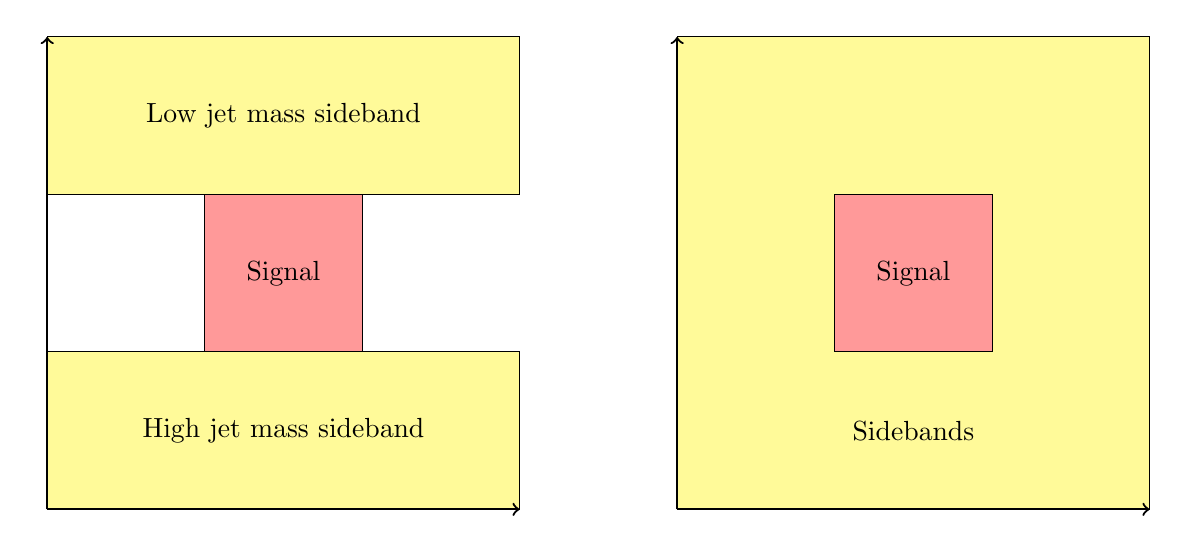
\begin{tikzpicture}
  % Jet mass sidebands
  \draw[fill=yellow!40] (0,0) rectangle (6,2) node[pos=0.5] {High jet mass sideband};
  \draw[fill=yellow!40] (0,4) rectangle (6,6) node[pos=0.5] {Low jet mass sideband};

  % Sidebands
  \draw[fill=yellow!40] (8,0) rectangle (14,6);
  \node at (11,1) {Sidebands};

  % Signal regions
  \draw[fill=red!40] (2,2) rectangle (4,4) node[pos=0.5] {Signal};
  \draw[fill=red!40] (10,2) rectangle (12,4) node[pos=0.5] {Signal};

  % Axes
  \draw[->,thick] (0,0) -- (6,0) node[below] {\MVV};
  \draw[->,thick] (0,0) -- (0,6) node[left] {\MJ};

  \draw[->,thick] (8,0) -- (14,0) node[below] {\MVV};
  \draw[->,thick] (8,0) -- (8,6) node[left] {\MJ};
\end{tikzpicture}

  \caption{
    Sideband regions of the fit for traditional sideband background estimation methods (left) versus the sideband regions in the 2D fit approach (right).
    The 2D fit method performs a simultaneous fit in the 2D sideband region in the \MVV-\MJ plane as opposed to modeling background in the \MVV and \MJ spectra in separate steps.
  }
  \label{fig:2Dfit}
\end{figure}

% Advantages of 2D fit
Thus, the 2D fit has the following advantages compared to the traditional $\alpha$ method previously used:
\begin{enumerate}
  \item The sideband as seen in figure~\ref{fig:2Dfit} is two-dimensional, thereby allowing for a simultaneous fit of the jet mass and resonance sidebands.
  This better constrains the background, which allows for better sensitivity of the search.
  \item The ability to add nuisance parameters that affect jet mass and resonance mass simultaneously, which allows us to account for the mismodeling of the correlation between the variables.
  \item Being able to use the full jet mass line-shape to extract the signal instead of using jet mass windows, providing better discrimination between $W$ and $Z$ peaks.
  \item Simultaneous fit of all \WV/\WH signals in the jet mass sideband, therefore allowing for easy implementation of exotic models such as heavy vector triplets.
\end{enumerate}

% Types of shapes in 2D fit
There are three types of shapes to consider for the 2D fit in the \MVV-\MJ plane.
The first is that of a signal process, for which we expect to see a resonance in both \MVV and \MJ.
In this case, the correlations are related to the scale and resolution of the jet.
For a background process in which there is a hadronically decaying boson (i.e., a $W$, $Z$, or $H$ from a \WVt process), we expect to observe a resonance in the \MJ dimension corresponding to the decay from the boson, but a falling spectrum in the \MVV dimension.
Lastly, if we instead have a QCD background process such as \Wjets, there will be a falling background distribution in both \MVV and \MJ, for which the shapes are correlated.

% Background types
As mentioned previously, two main classes of background are considered for this analysis, as classified based on resonant or non-resonant behavior in the \MJ spectrum:
\begin{itemize}
  \item \textbf{Resonant:} Background events in which the jet mass shape is peaking as a $W$, $Z$, $H$, or $t$ resonance in \MJ with a falling spectrum in \MVV.
  The resonant peak in \MJ is due to partially or fully merged top jets and diboson events in which one boosted boson is reconstructed into a jet.
  The main contribution is \WVt events.
  \item \textbf{Non-resonant:} Background events in which the jet is produced by the hadronization of one or more partons not originating from a vector boson.
  The dominant SM contribution is from \Wjets events, but additional contributions come from $t\bar{t}$ events as well.
\end{itemize}

% Merging samples for Run 2
The templates are derived from MC samples for both signal and background as enumerated in section~\ref{sec:samples}.
These samples were created in successive campaigns over 2016, 2017, and 2018, and are separated by their production year.
Previous versions of this analysis kept the templates separated by year, but for this iteration of the analysis we merge the samples for all three years and weight them by their respective luminosities to obtain combined Run 2 samples.
This has the benefit of providing better modeling of templates in categories with low statistics.

\subsection{Signal Modeling}
\label{sec:sig}

% Signal overview
Because the MC samples for the various signals used in the analysis only sample several points for the resonance mass \MX, we employ interpolation methods to model the signal for any arbitrary resonance mass \MX within the range 0.8-$4.5\unit{TeV}$.
To do so, we derive the each of the parameters for the signal shapes as functions of \MX, as well as the signal yield per pb of cross section as a function of \MX.

\subsubsection{Signal Shapes}

% Signal shapes
Each signal model takes the same functional form in the two-dimensional \MJ-\MVV space.
The signals are parameterized in 2D as the product of the two 1D \MJ and \MVV shapes for the jet mass and the resonance mass given by
\begin{equation}
  P_\mathrm{sig}(\MVV,\MJ|\MX)=\PVV(\MVV|\MX,\vb*{\theta}_1)\PJ(\MJ|\MX,\vb*{\theta}_2),
\end{equation}
where $\vb*{\theta}_1$ and $\vb*{\theta}_2$ are shape parameters that in principle depend on \MX.
Both shapes are modeled separately based on the jet purity (HP/LP), rapidity (HDy/LDy), and bb/nobb/vbf categories.
However, the $e$ and $\mu$ categories are merged for the signal modeling process.
To parameterize the shapes, we perform separate fits for the 1D shapes in the \MVV and \MJ spectra, then interpolate the parameters for each shape as a function of \MX to obtain $P_\mathrm{sig}(\MVV,\MJ|\MX)$ for arbitrary \MX between 1 and $4.5\unit{TeV}$.
A DCB shape is used for $\PVV(\MVV|\MX,\vb*{\theta}_1)$ for all categories, while the jet resonance shape $\PJ(\MJ|\MX,\vb*{\theta}_2)$ uses a DCB for the HP categories, and the sum of a DCB and an exponential for the LP categories.

% Signal shape parameter figures
Figures~\ref{fig:MVVShapeParam_LDy_Run2} and \ref{fig:MVVShapeParam_HDy_Run2} show the DCB parameters ($\mu$, $\sigma$, $\alpha_1$, $\alpha_2$) for the \MVV shapes in the 12 categories used to model the 2D signal shapes.
The DCB parameters for the \MJ shapes are shown in figures~\ref{fig:MJJShapeParam_LDy_Run2} and \ref{fig:MJJShapeParam_HDy_Run2}

% Signal shape substitutions
In some categories there are not enough events present that result in a smooth fit for the parameters of $\PVV(\MVV|\MX,\vb*{\theta}_1)$ or $\PJ(\MJ|\MX,\vb*{\theta}_2)$.
For example, signals that are \VBF-produced will not have a sufficient number of events present for the bb/nobb categories.
Because the signal parameters do not vary significantly between production modes, we allow for substituting non-\VBF signal shapes with \VBF shapes, and \VBF signal shapes with non-\VBF shapes:
\begin{itemize}
  \item \VBF\ZprtoWW shapes are used for \DY\ZprtoWW in the vbf categories.
  \item \VBF\WprtoWH shapes are used for \DY\WprtoWH in the vbf categories.
  \item \VBF\WprtoWZ shapes are used for \DY\WprtoWZ in the vbf categories.
  \item \ggF\GBulktoWW shapes are used for \VBF\GBulktoWW in the bb categories.
  \item \DY\WprtoWZ shapes are used for \VBF\WprtoWZ in the bb and nobb categories.
  \item \ggF\RadtoWW shapes are used for \VBF\RadtoWW in the LP-bb categories.
  \item \ggF\GBulktoWW \MJ shapes are used for \DY\ZprtoWW \MJ in the LP-bb categories.
  \item \DY\ZprtoWW shapes are used for \VBF\ZprtoWW in the bb-LDy categories.
\end{itemize}

% Analytic signal shape figures
Figures \ref{fig:MVVShapes_NonVBF_LDy_Run2} and \ref{fig:MVVShapes_NonVBF_HDy_Run2} show the \MVV signal shapes for non-\VBF signals.
For figures \ref{fig:MVVShapes_VBF_LDy_Run2} and \ref{fig:MVVShapes_VBF_HDy_Run2}, we show the \MVV signal shapes for the \VBF signals.
In figures \ref{fig:MJJShapes_NonVBF_LDy_Run2} and \ref{fig:MJJShapes_NonVBF_HDy_Run2}, the \MJ signal shapes are shown for the non-\VBF signals.
Finally, figures \ref{fig:MJJShapes_VBF_LDy_Run2} and \ref{fig:MJJShapes_VBF_HDy_Run2} show the \MJ signal shapes for the \VBF signals.

\begin{figure}[htbp]
  \centering
  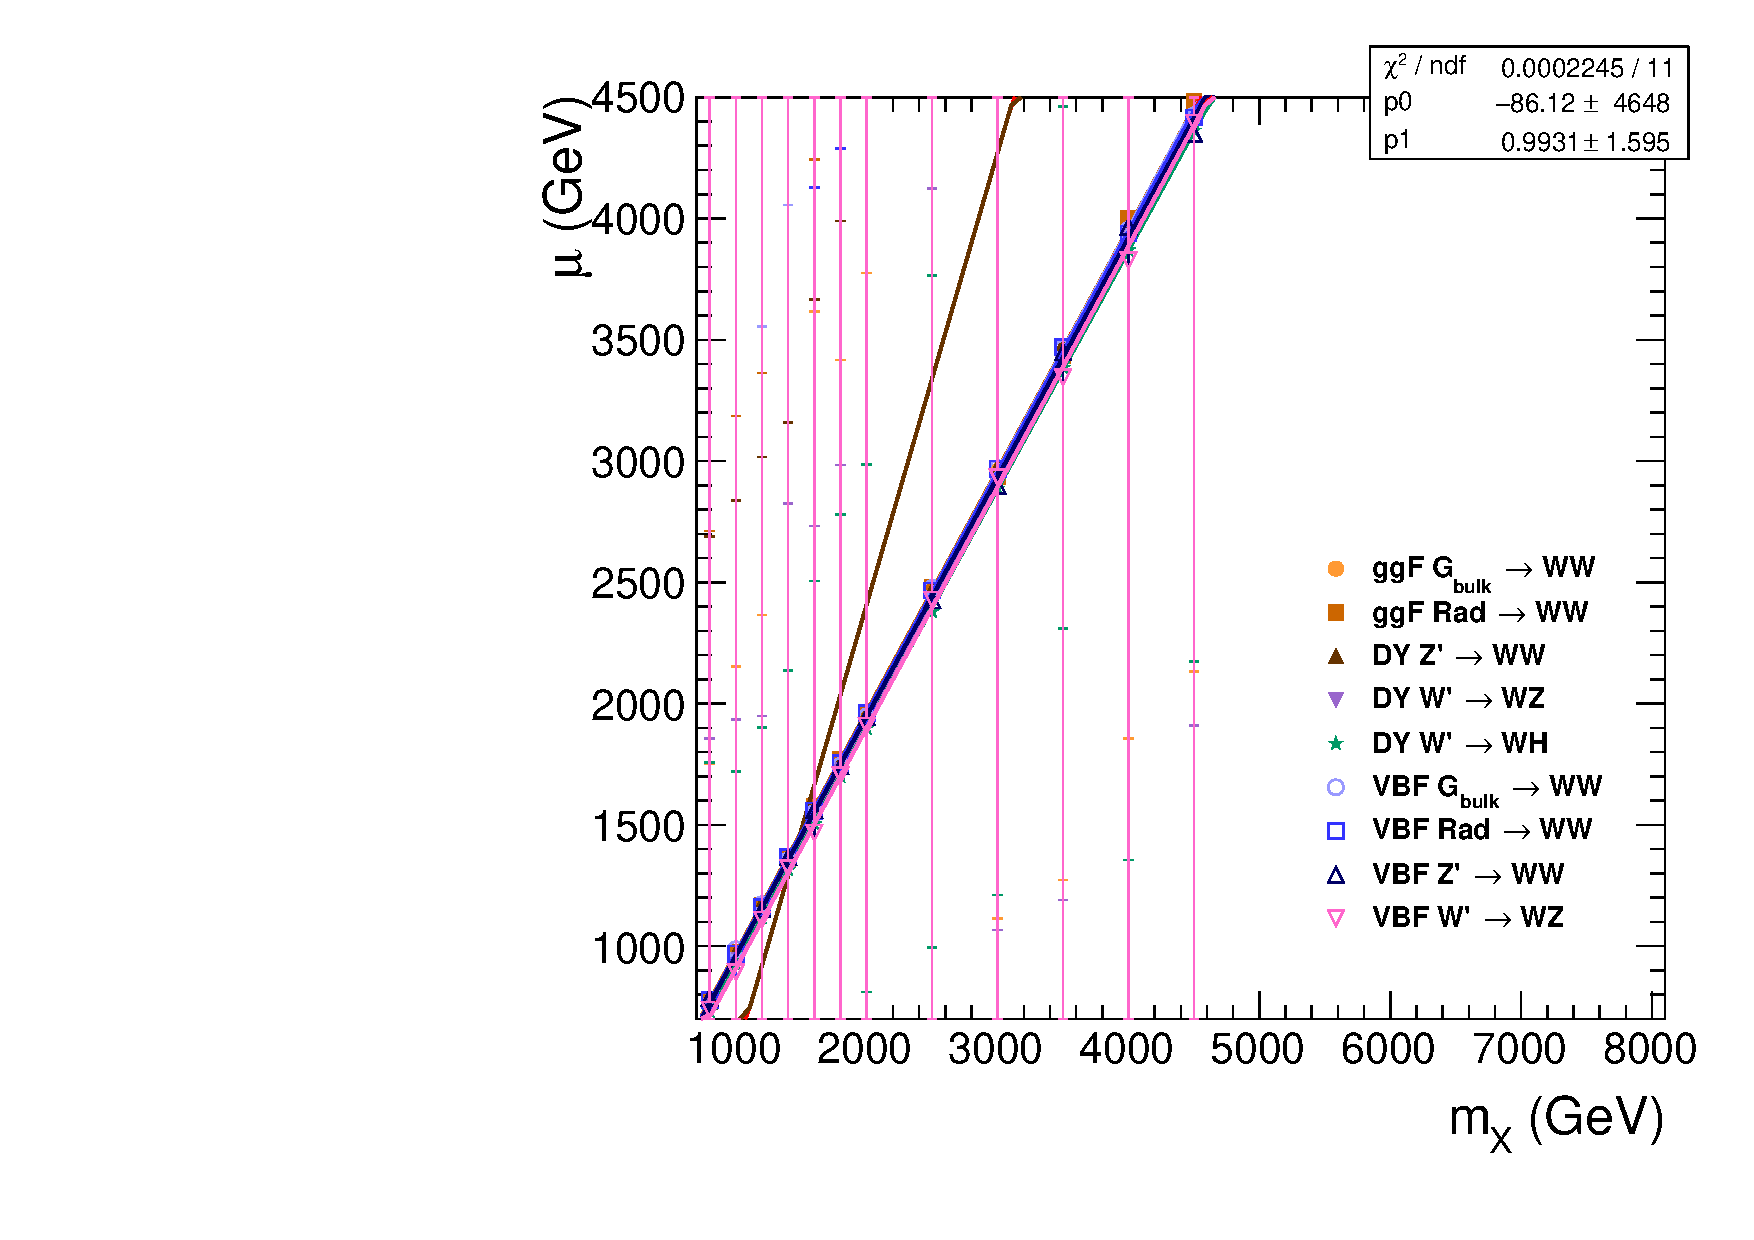
\includegraphics[width=0.2\textwidth]{fig/2Dfit/paramSignalShape_allSig_MVV_HP_bb_LDy_MEAN.pdf}
  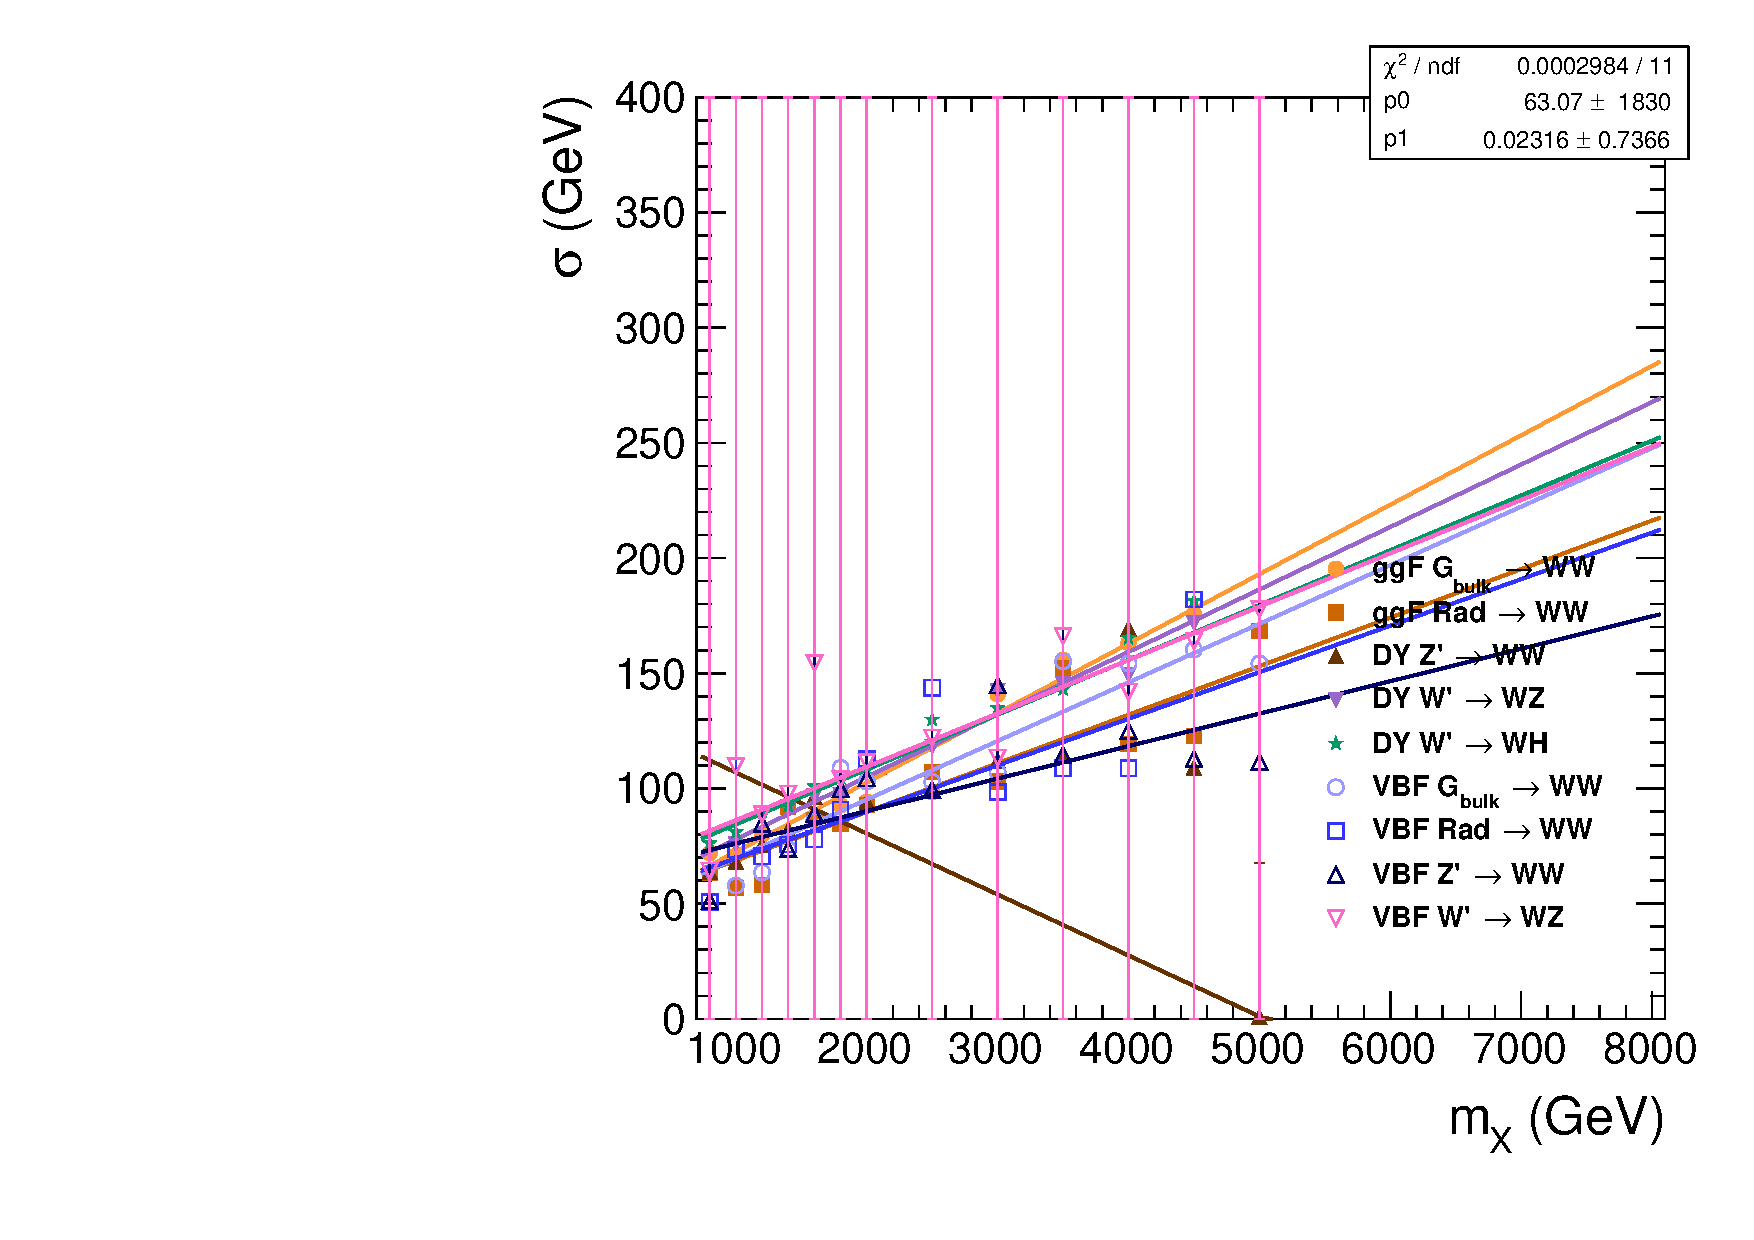
\includegraphics[width=0.2\textwidth]{fig/2Dfit/paramSignalShape_allSig_MVV_HP_bb_LDy_SIGMA.pdf}
  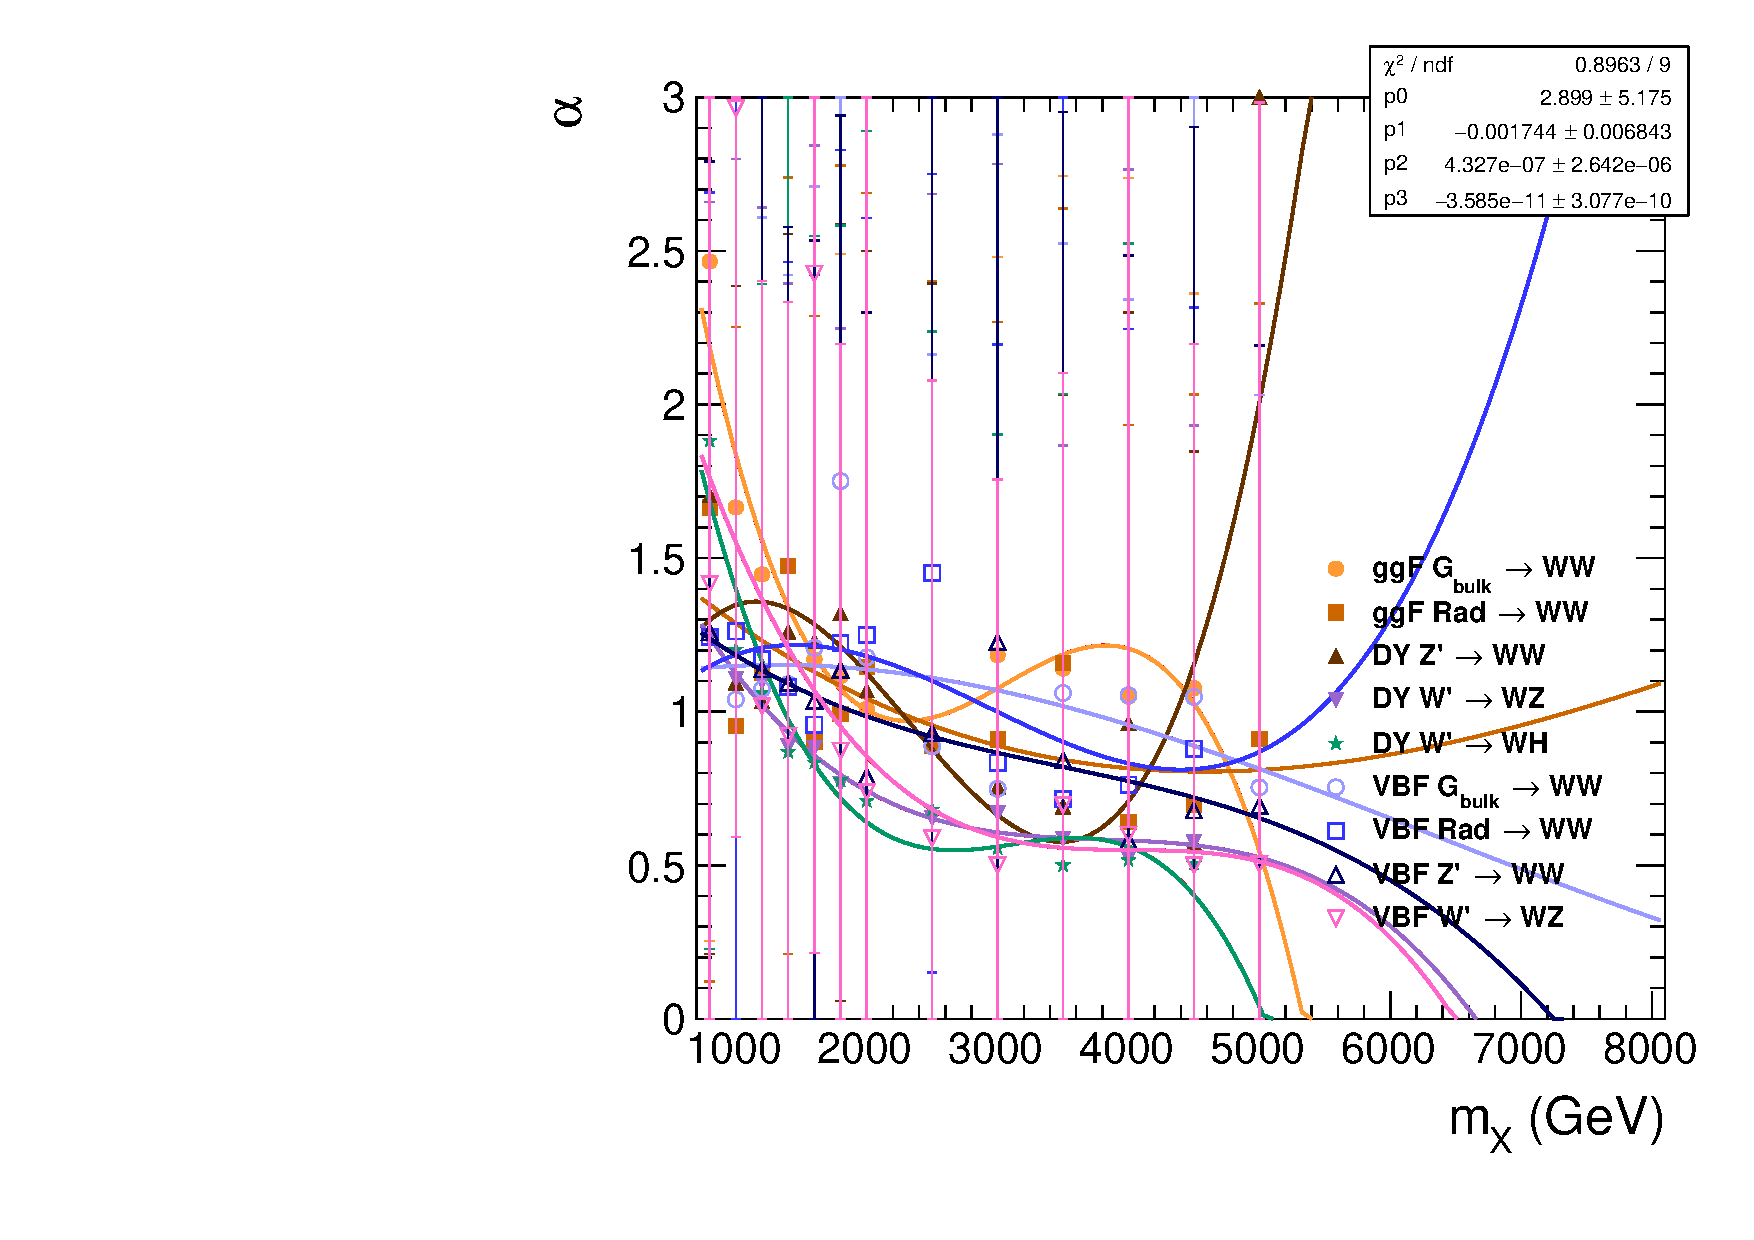
\includegraphics[width=0.2\textwidth]{fig/2Dfit/paramSignalShape_allSig_MVV_HP_bb_LDy_ALPHA1.pdf}
  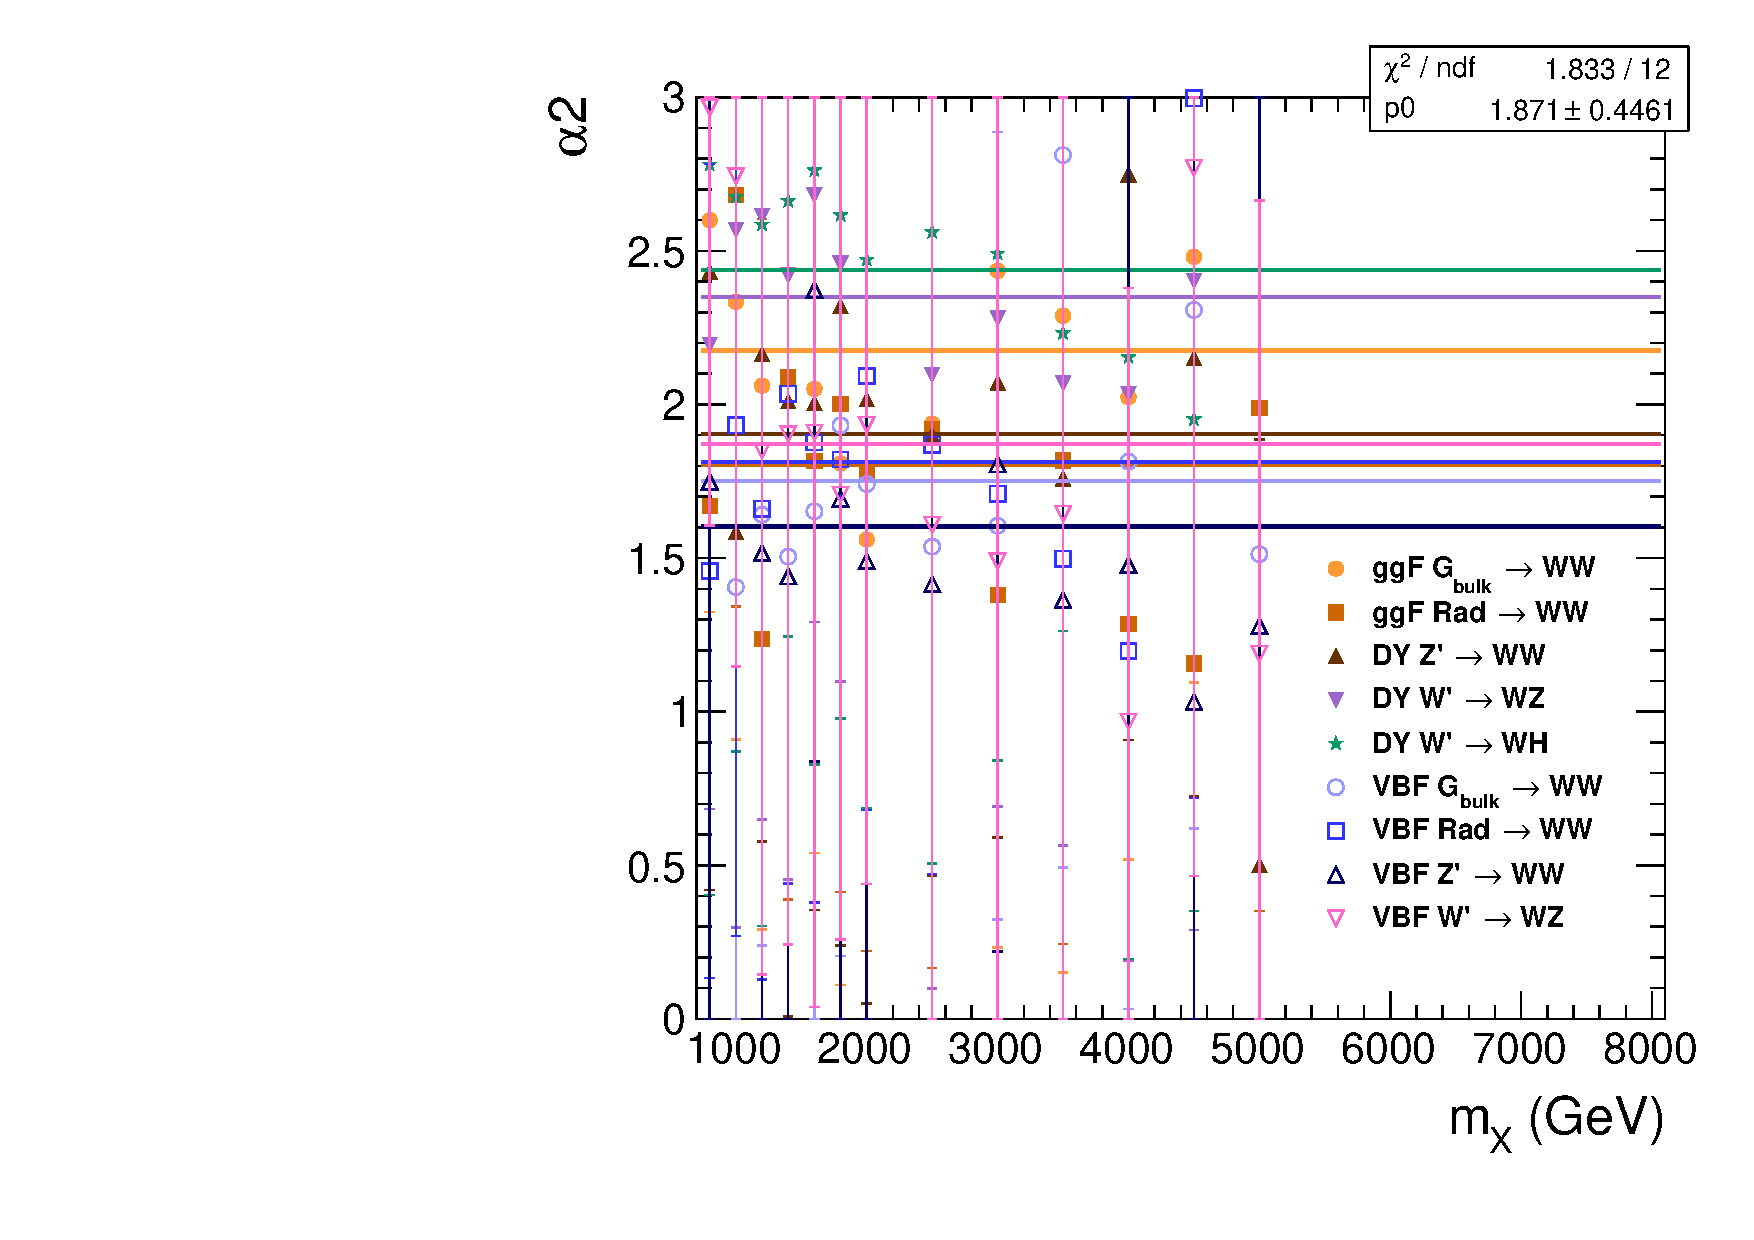
\includegraphics[width=0.2\textwidth]{fig/2Dfit/paramSignalShape_allSig_MVV_HP_bb_LDy_ALPHA2.pdf}\\
  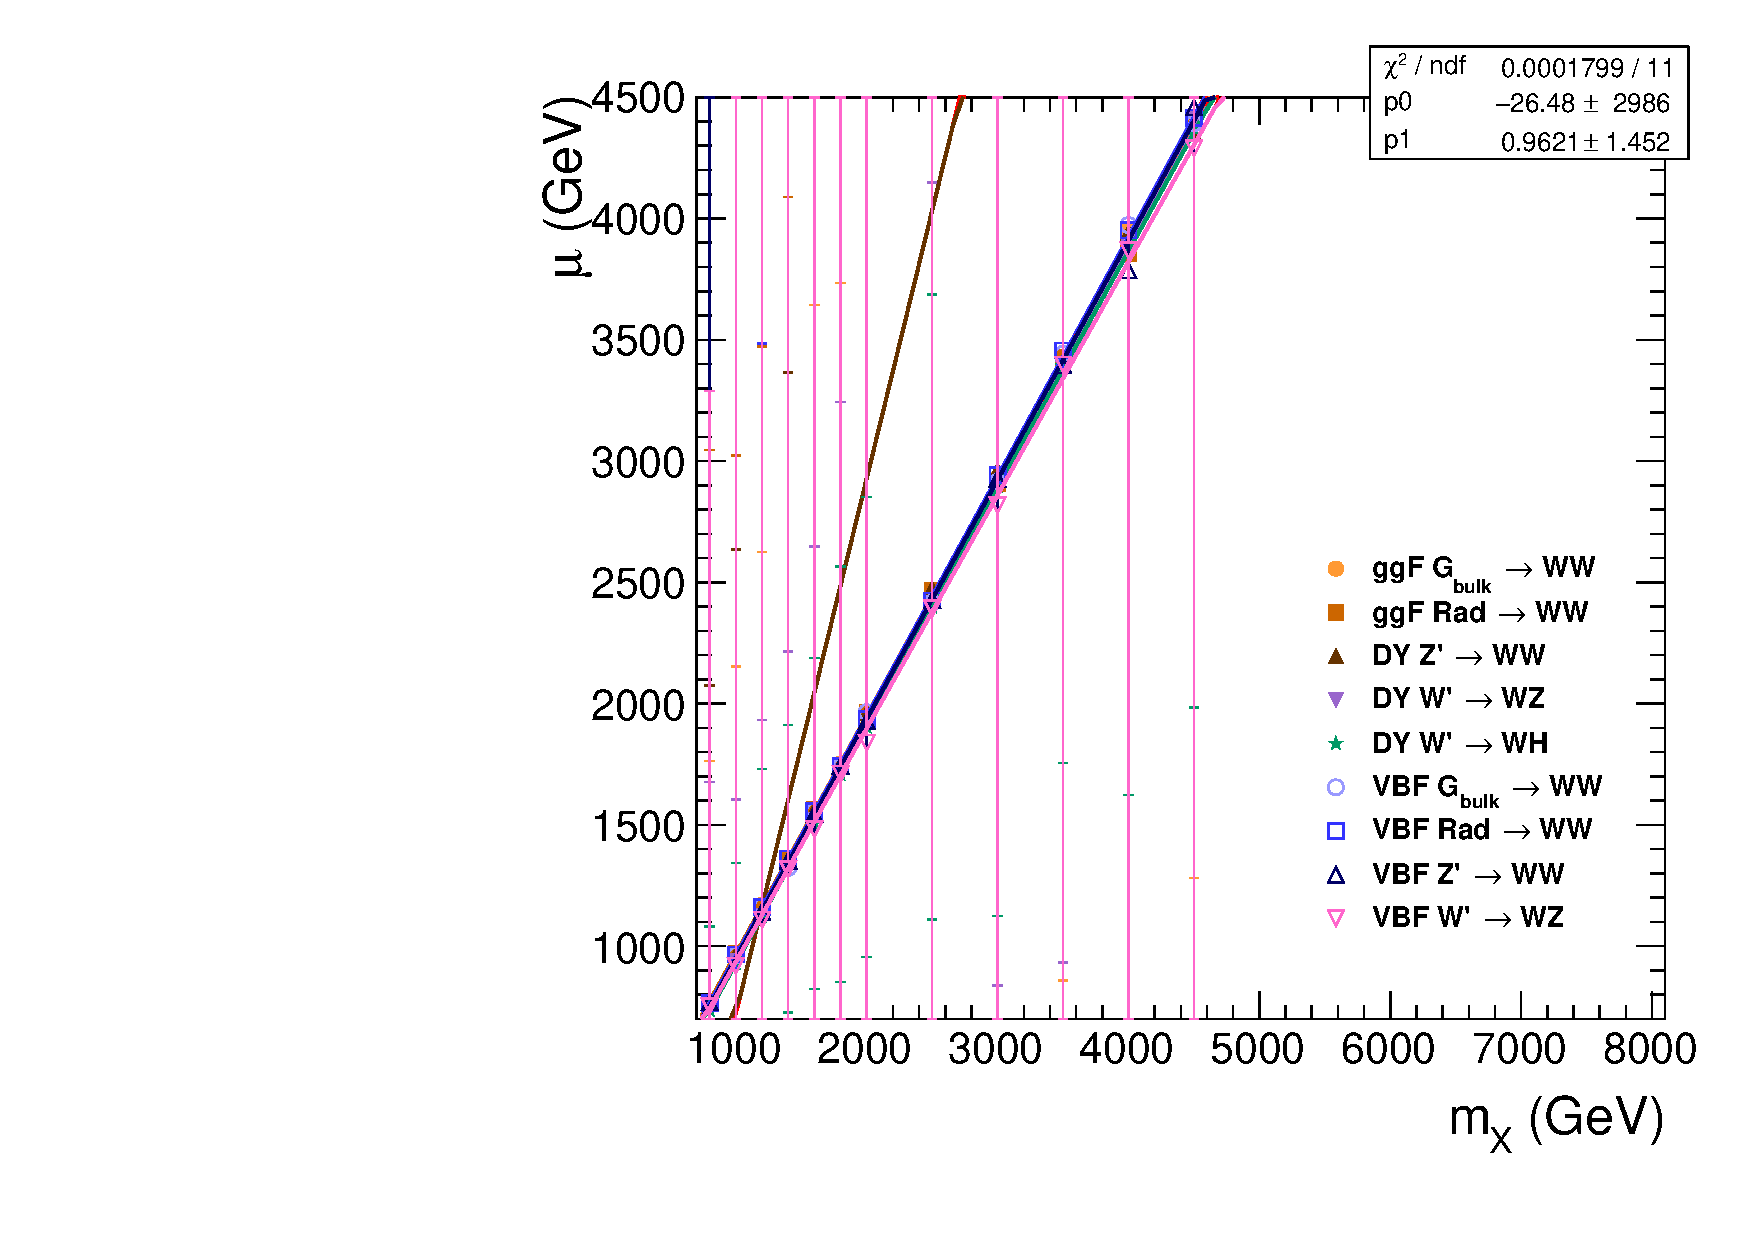
\includegraphics[width=0.2\textwidth]{fig/2Dfit/paramSignalShape_allSig_MVV_LP_bb_LDy_MEAN.pdf}
  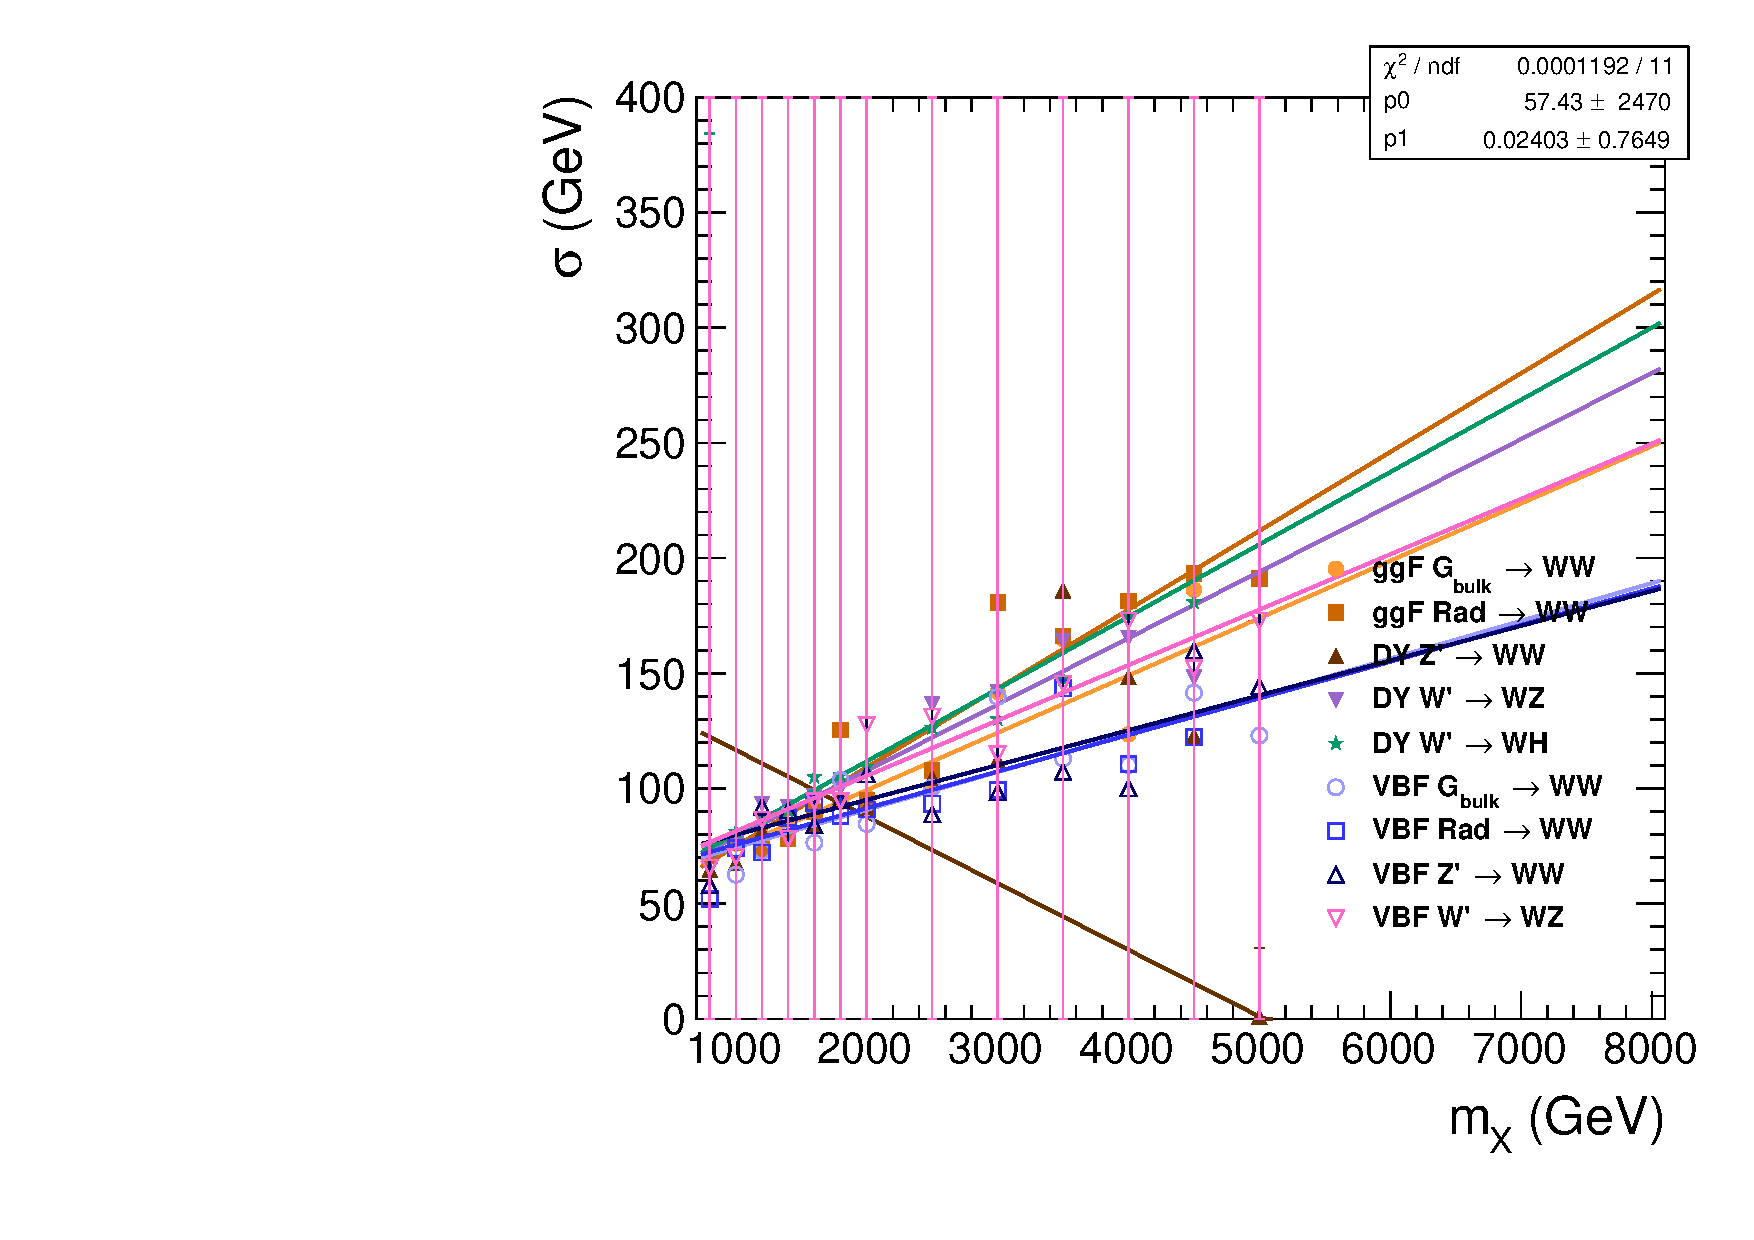
\includegraphics[width=0.2\textwidth]{fig/2Dfit/paramSignalShape_allSig_MVV_LP_bb_LDy_SIGMA.pdf}
  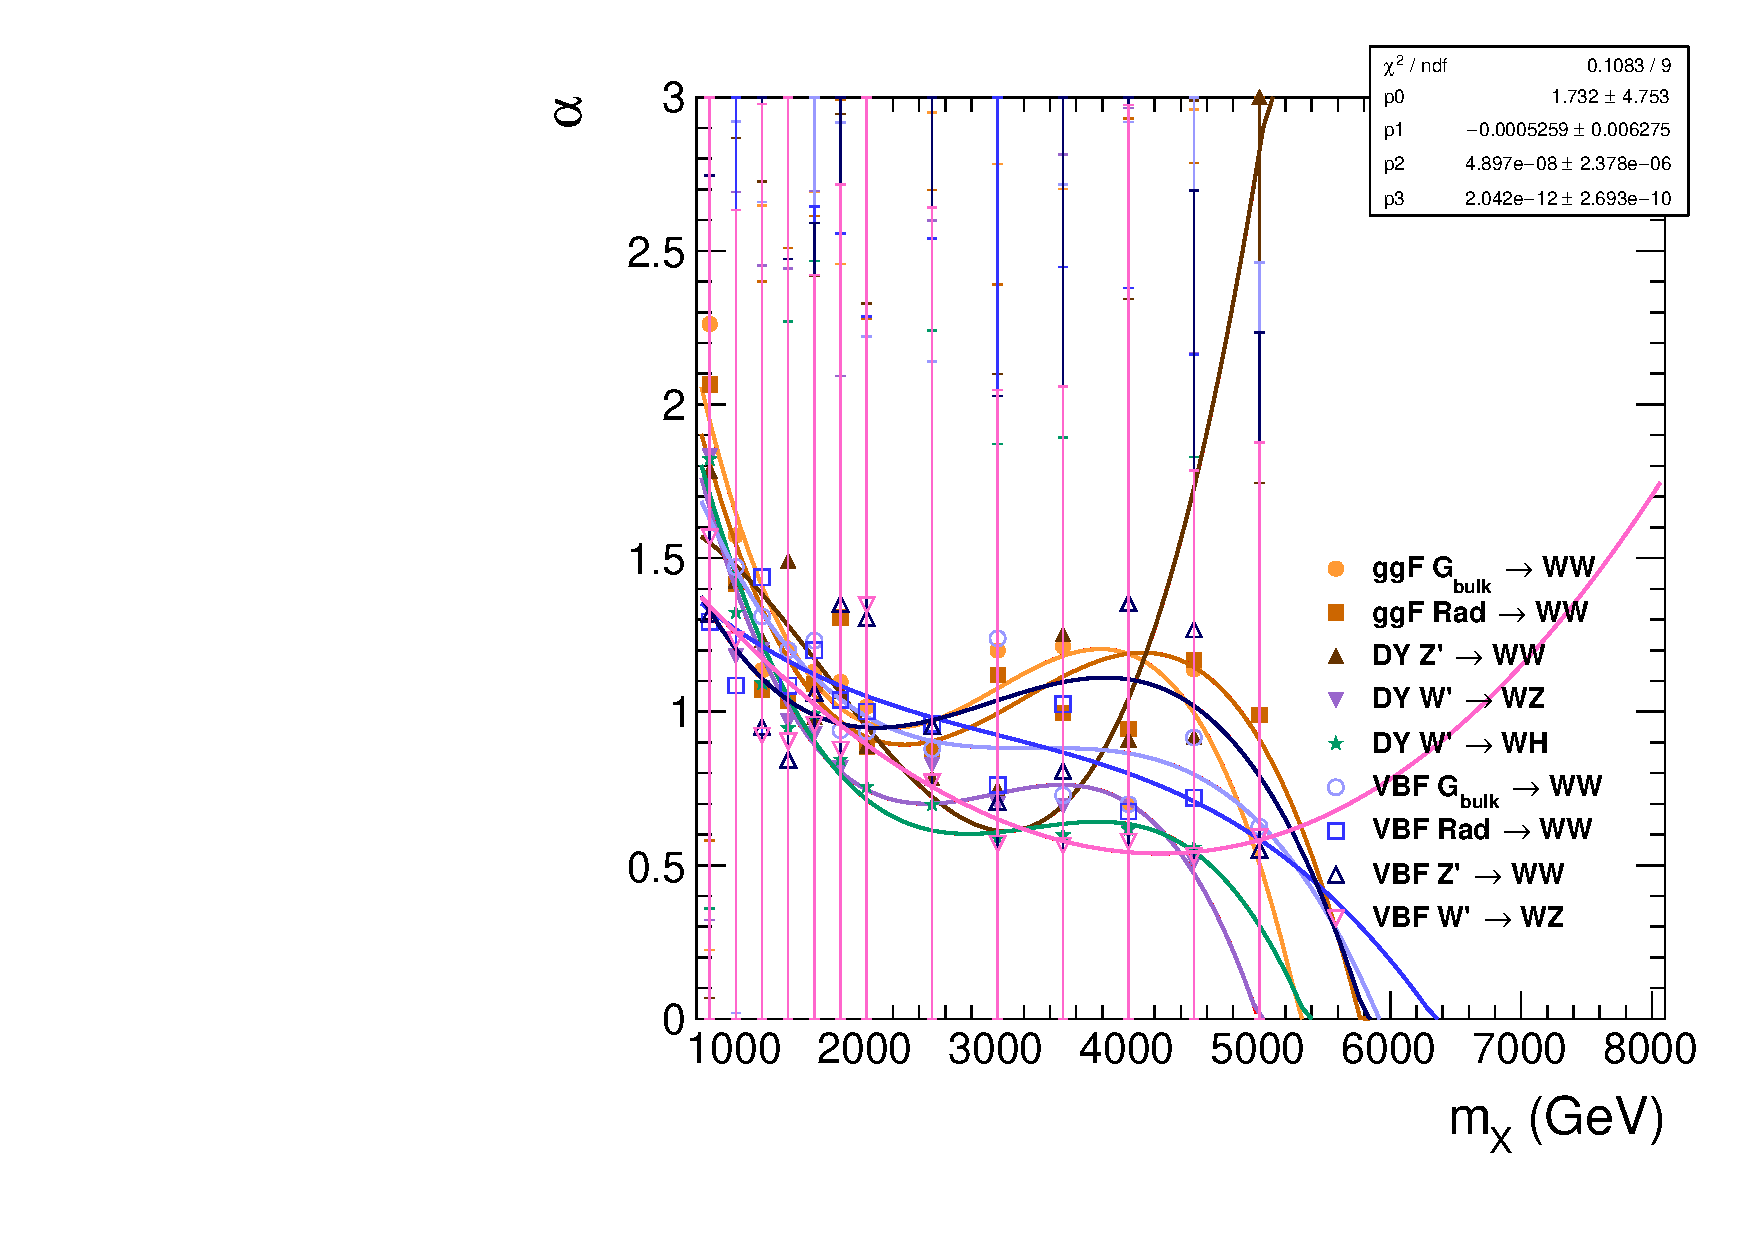
\includegraphics[width=0.2\textwidth]{fig/2Dfit/paramSignalShape_allSig_MVV_LP_bb_LDy_ALPHA1.pdf}
  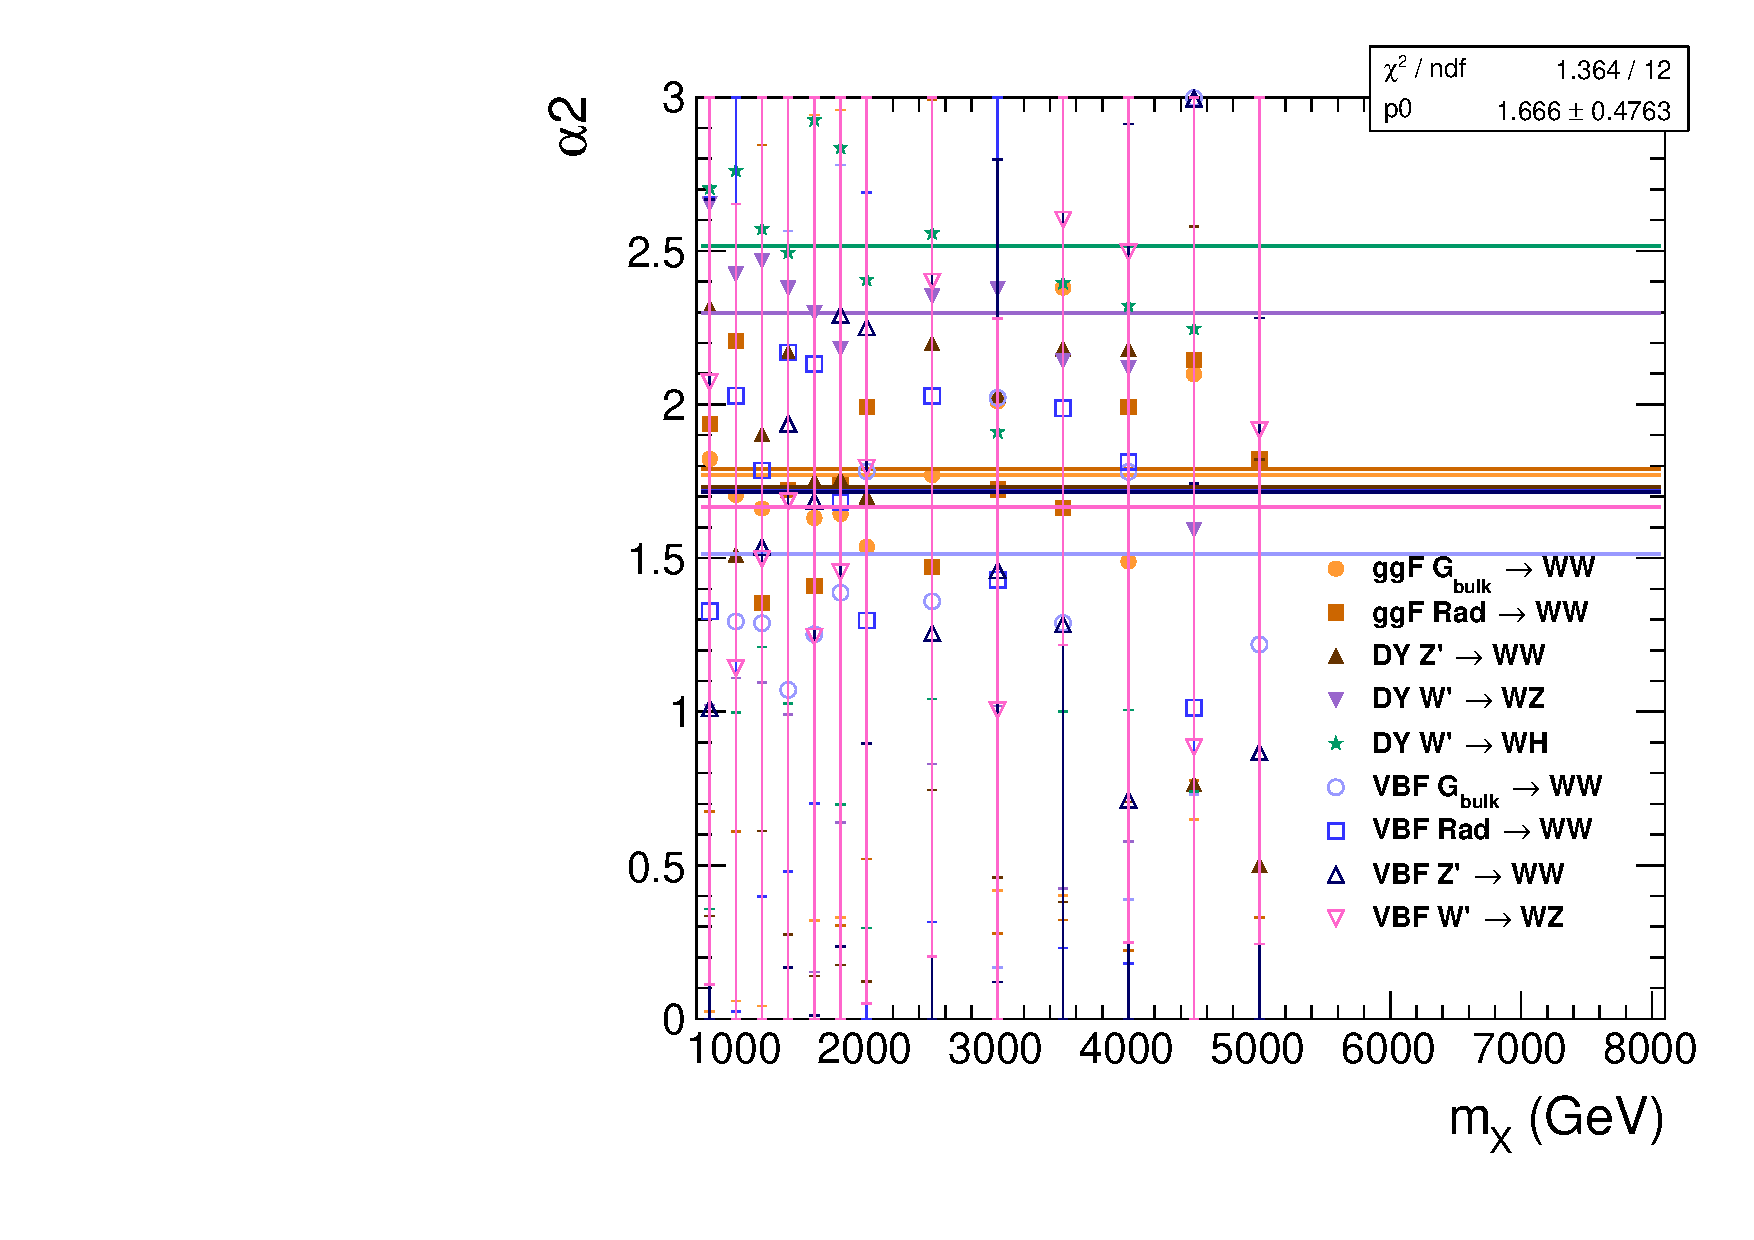
\includegraphics[width=0.2\textwidth]{fig/2Dfit/paramSignalShape_allSig_MVV_LP_bb_LDy_ALPHA2.pdf}\\
  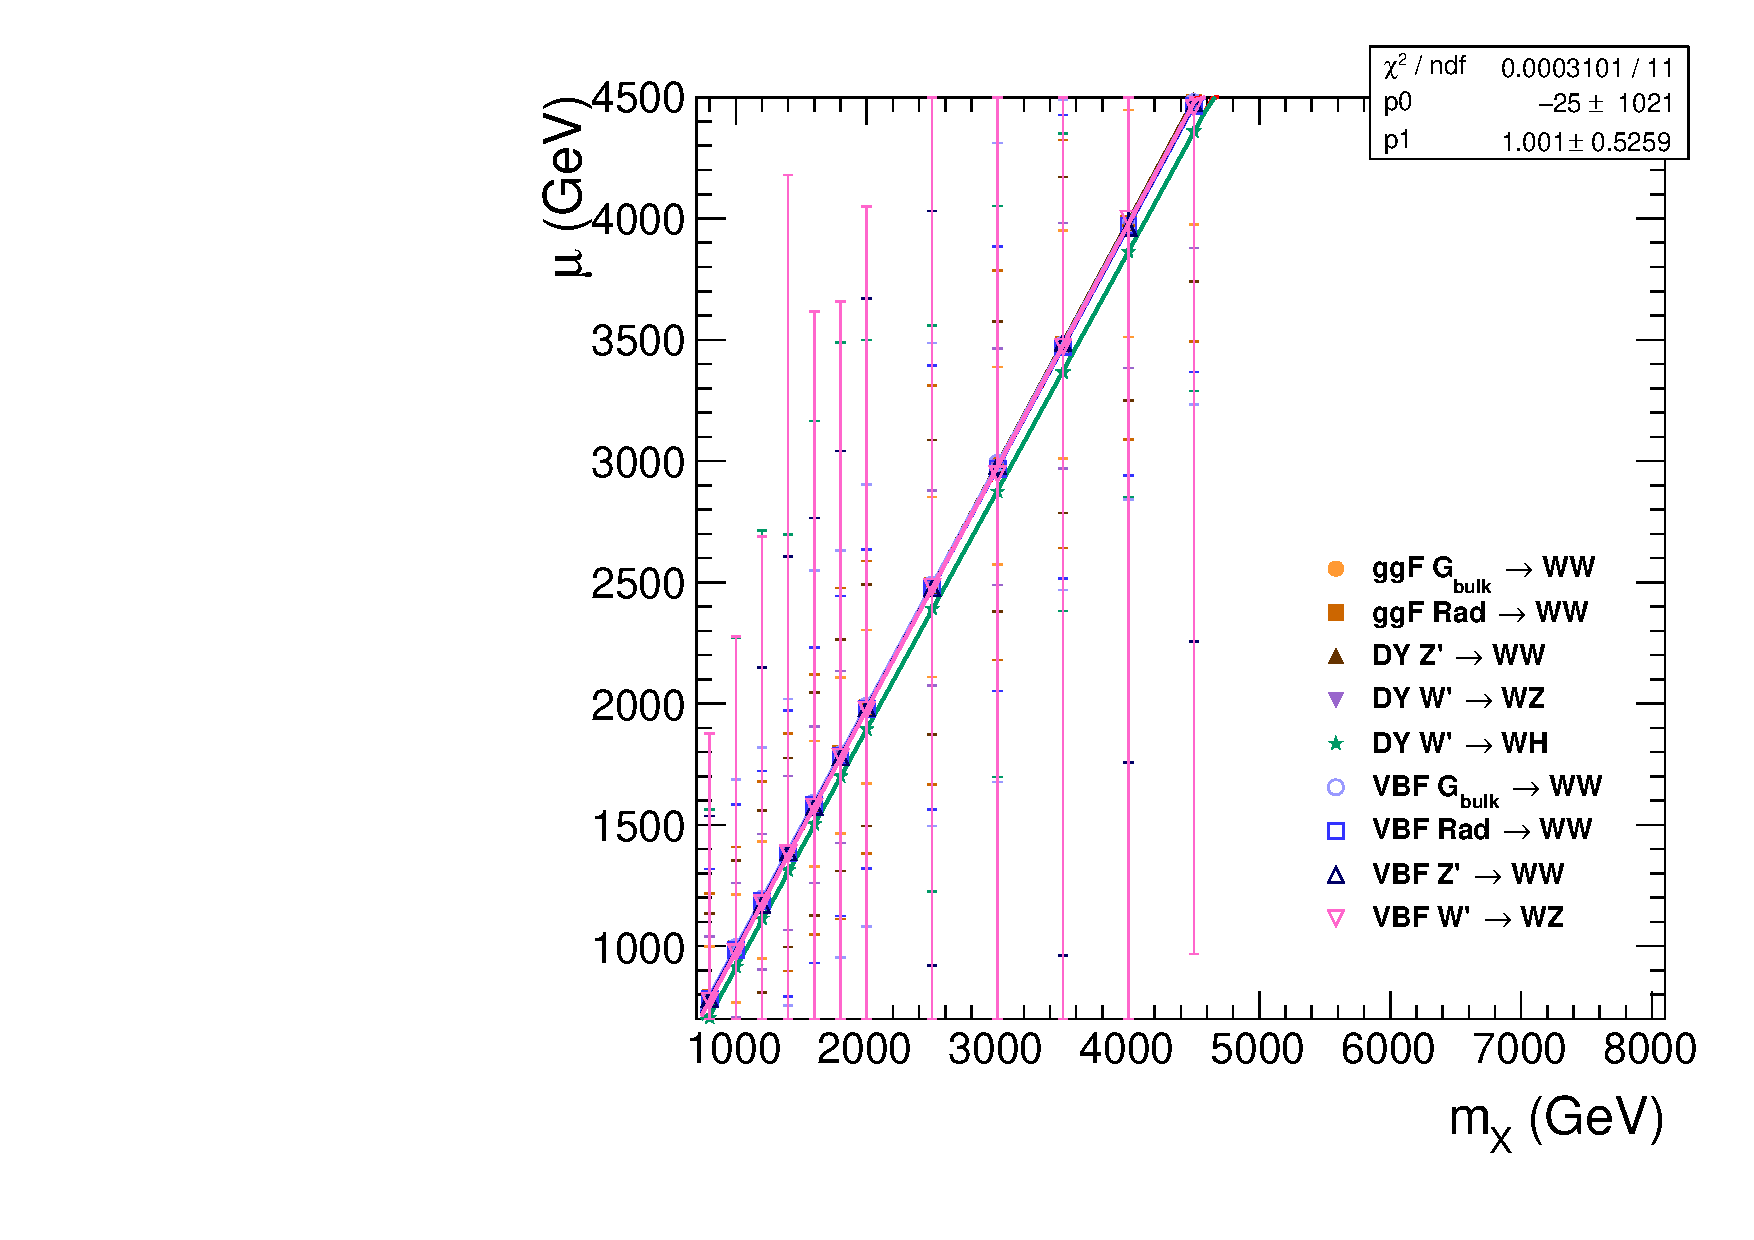
\includegraphics[width=0.2\textwidth]{fig/2Dfit/paramSignalShape_allSig_MVV_HP_nobb_LDy_MEAN.pdf}
  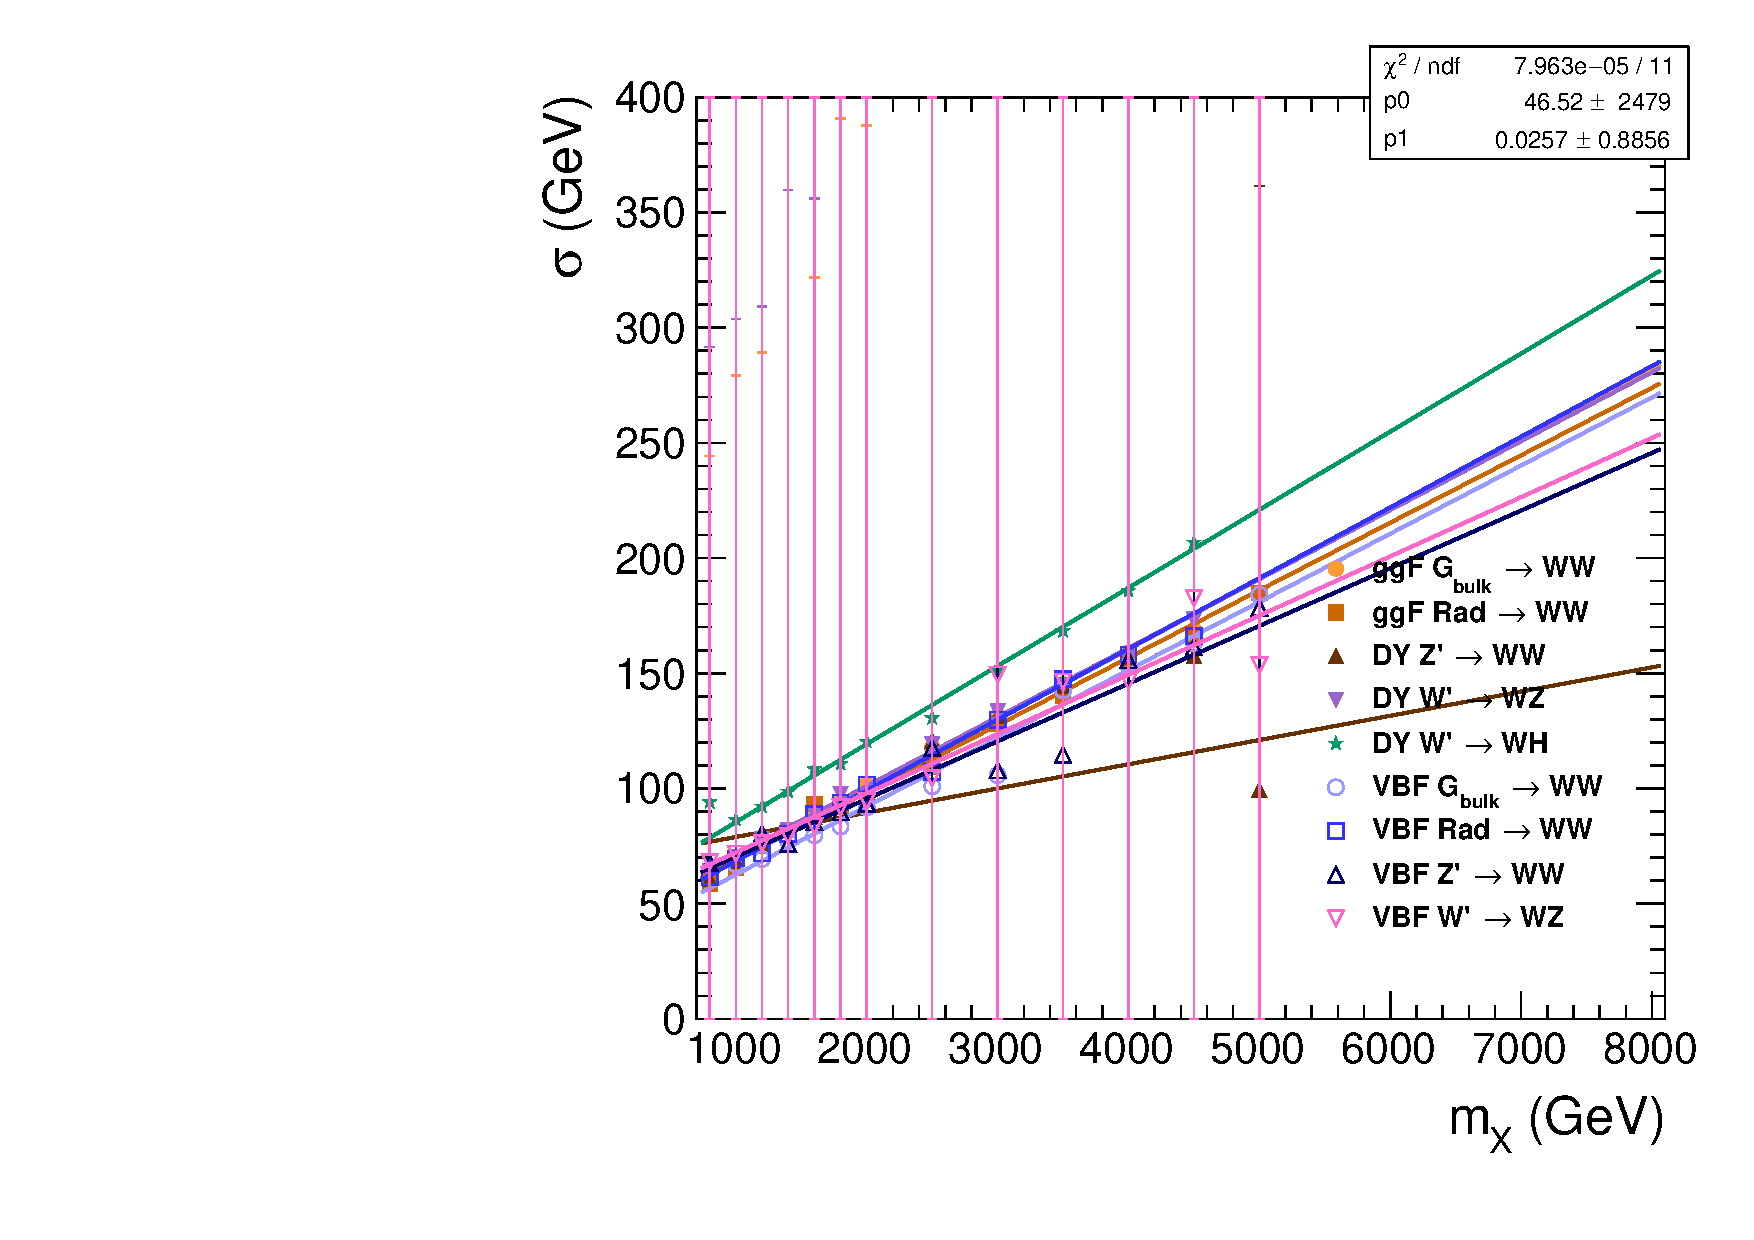
\includegraphics[width=0.2\textwidth]{fig/2Dfit/paramSignalShape_allSig_MVV_HP_nobb_LDy_SIGMA.pdf}
  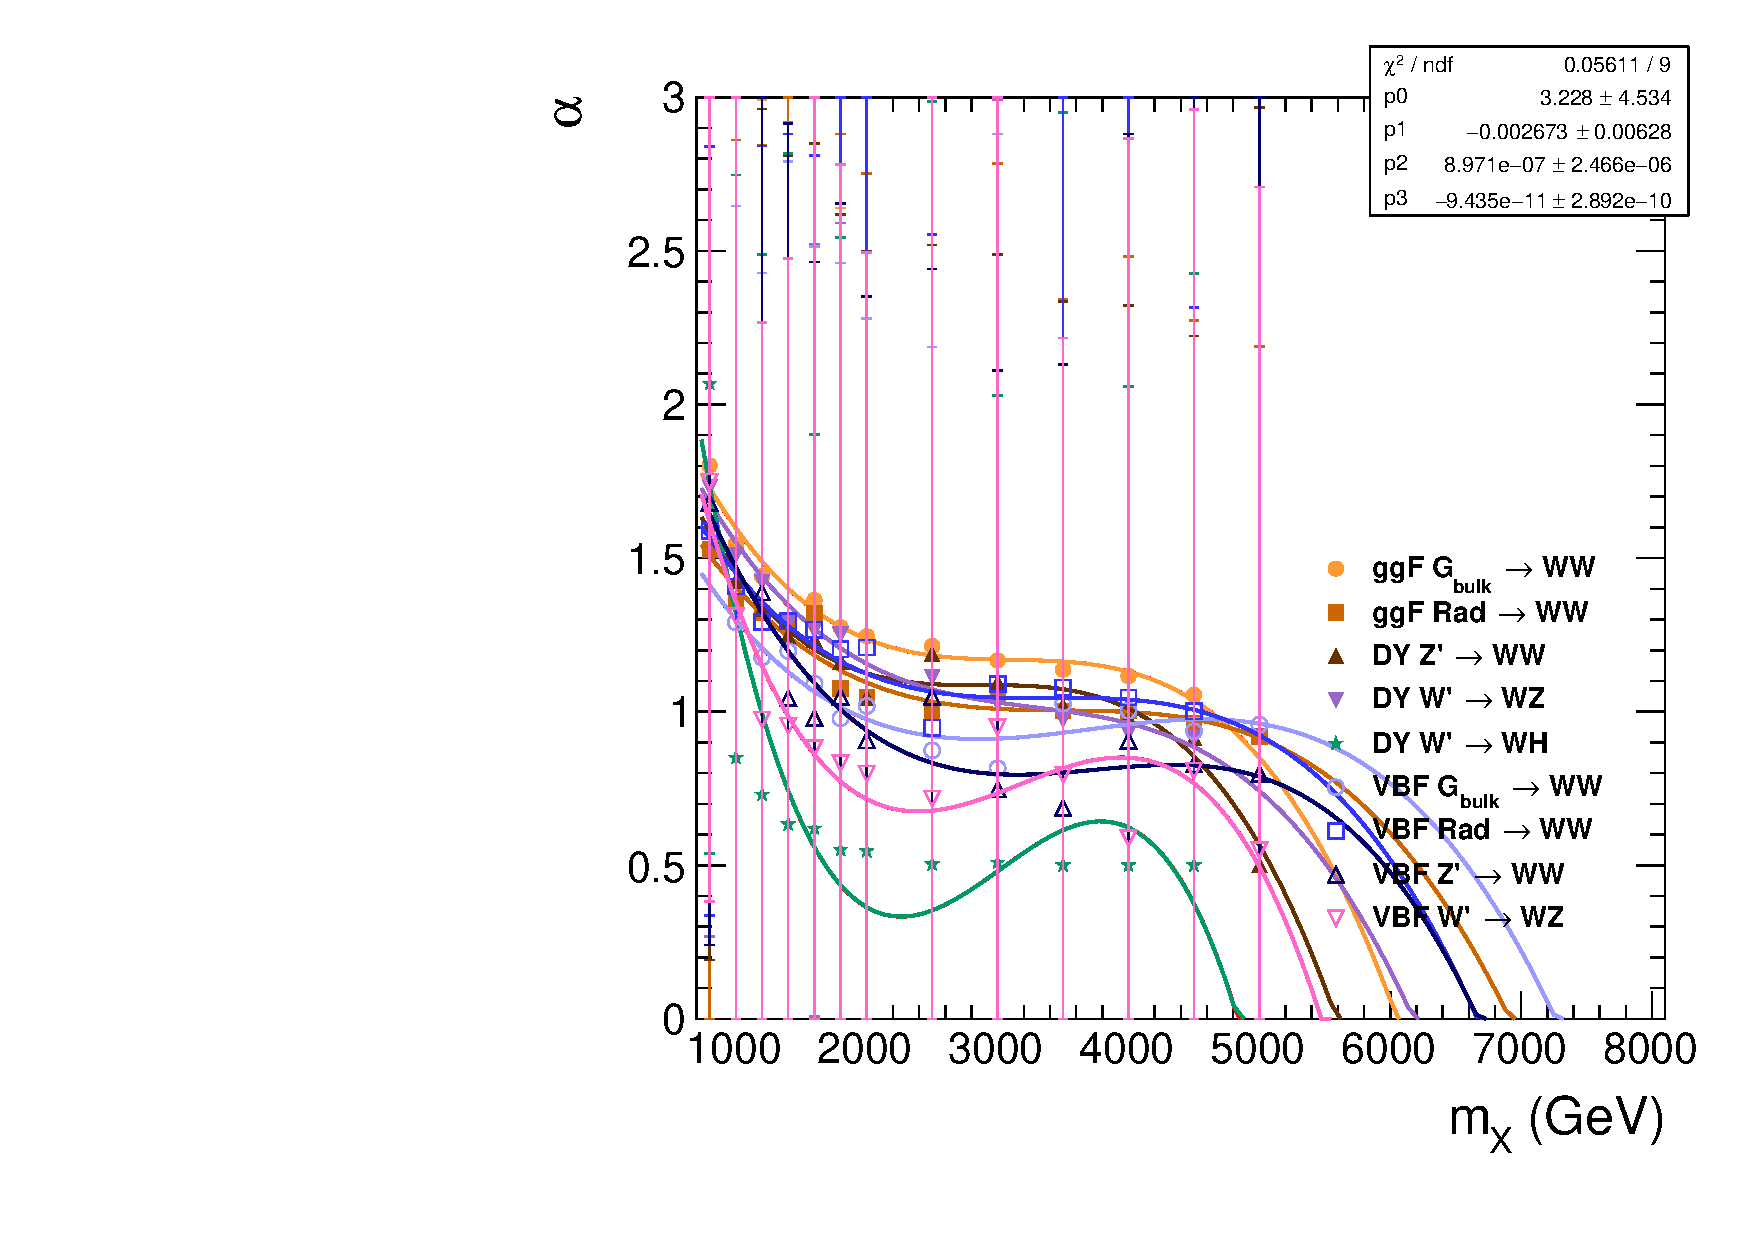
\includegraphics[width=0.2\textwidth]{fig/2Dfit/paramSignalShape_allSig_MVV_HP_nobb_LDy_ALPHA1.pdf}
  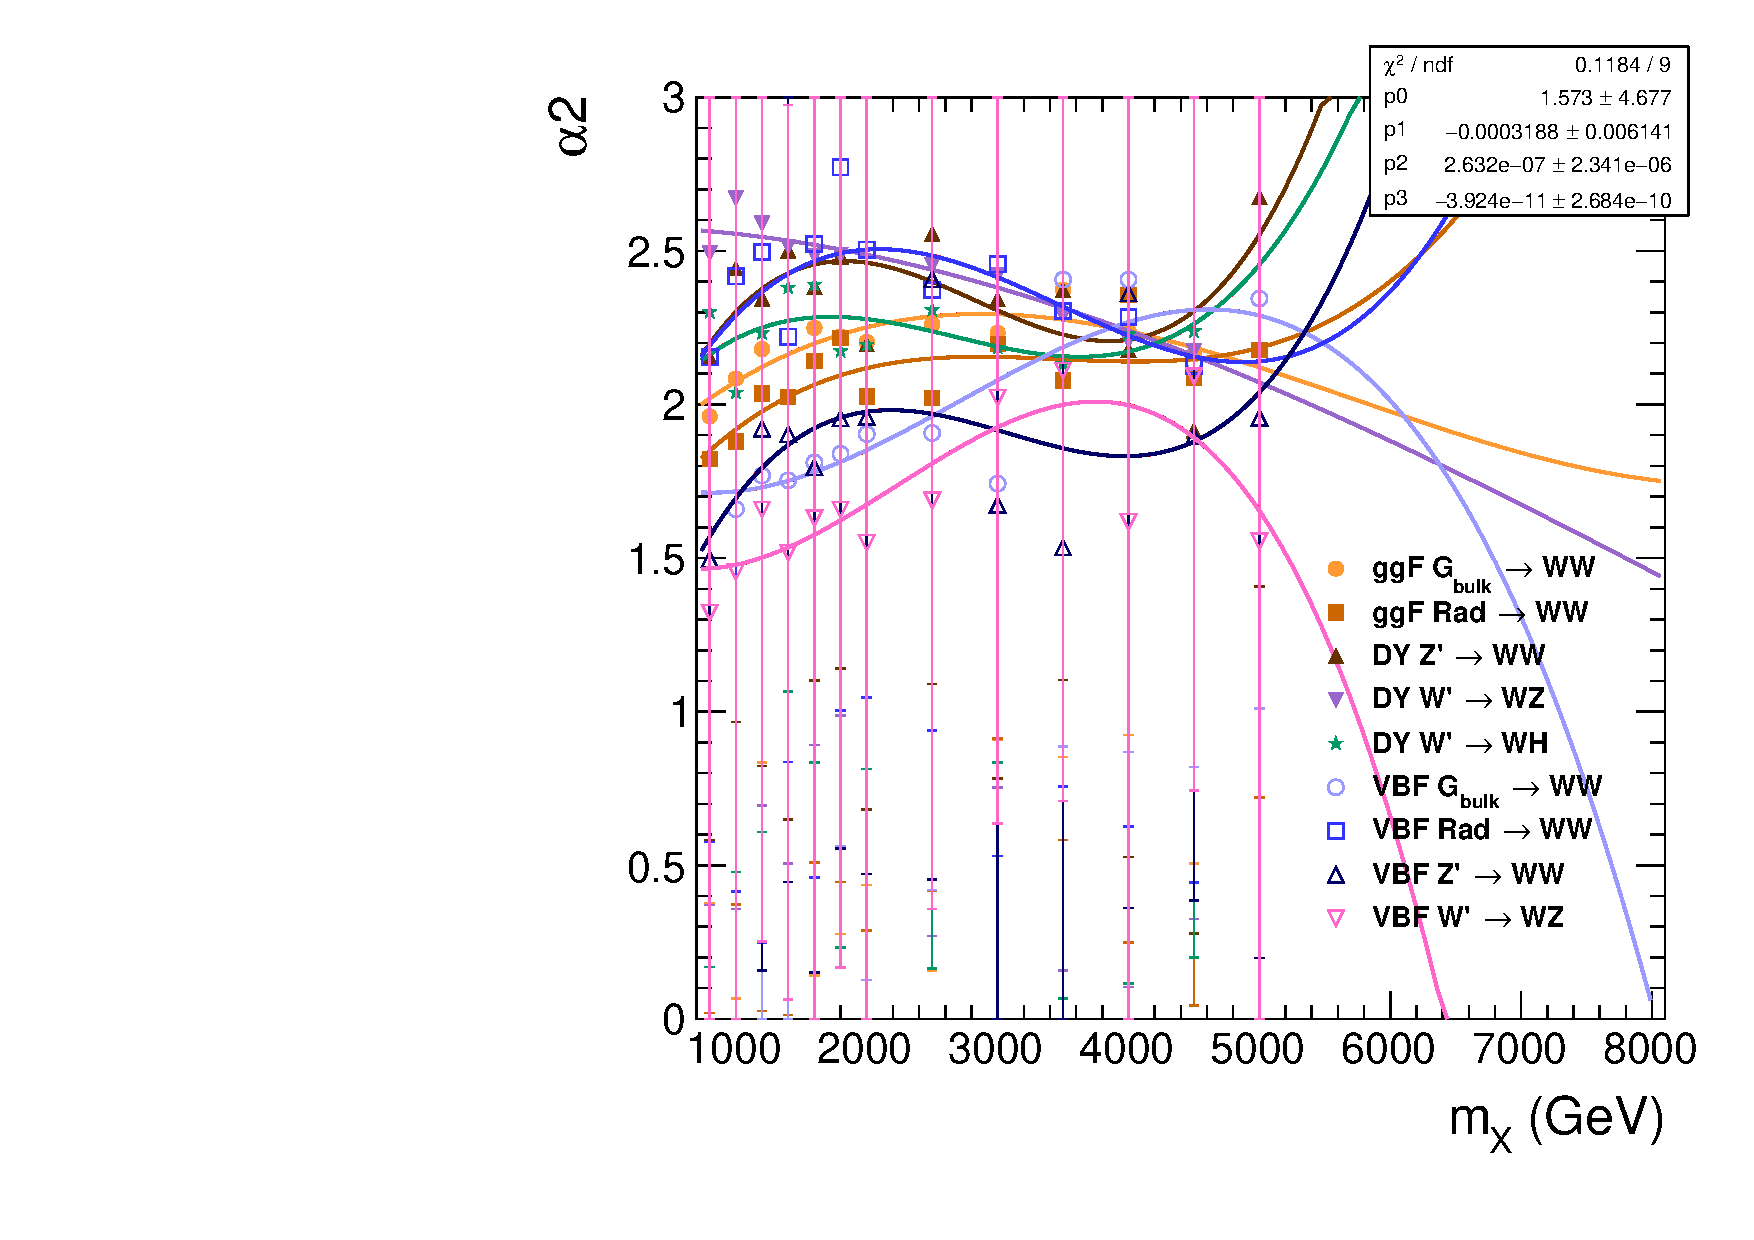
\includegraphics[width=0.2\textwidth]{fig/2Dfit/paramSignalShape_allSig_MVV_HP_nobb_LDy_ALPHA2.pdf}\\
  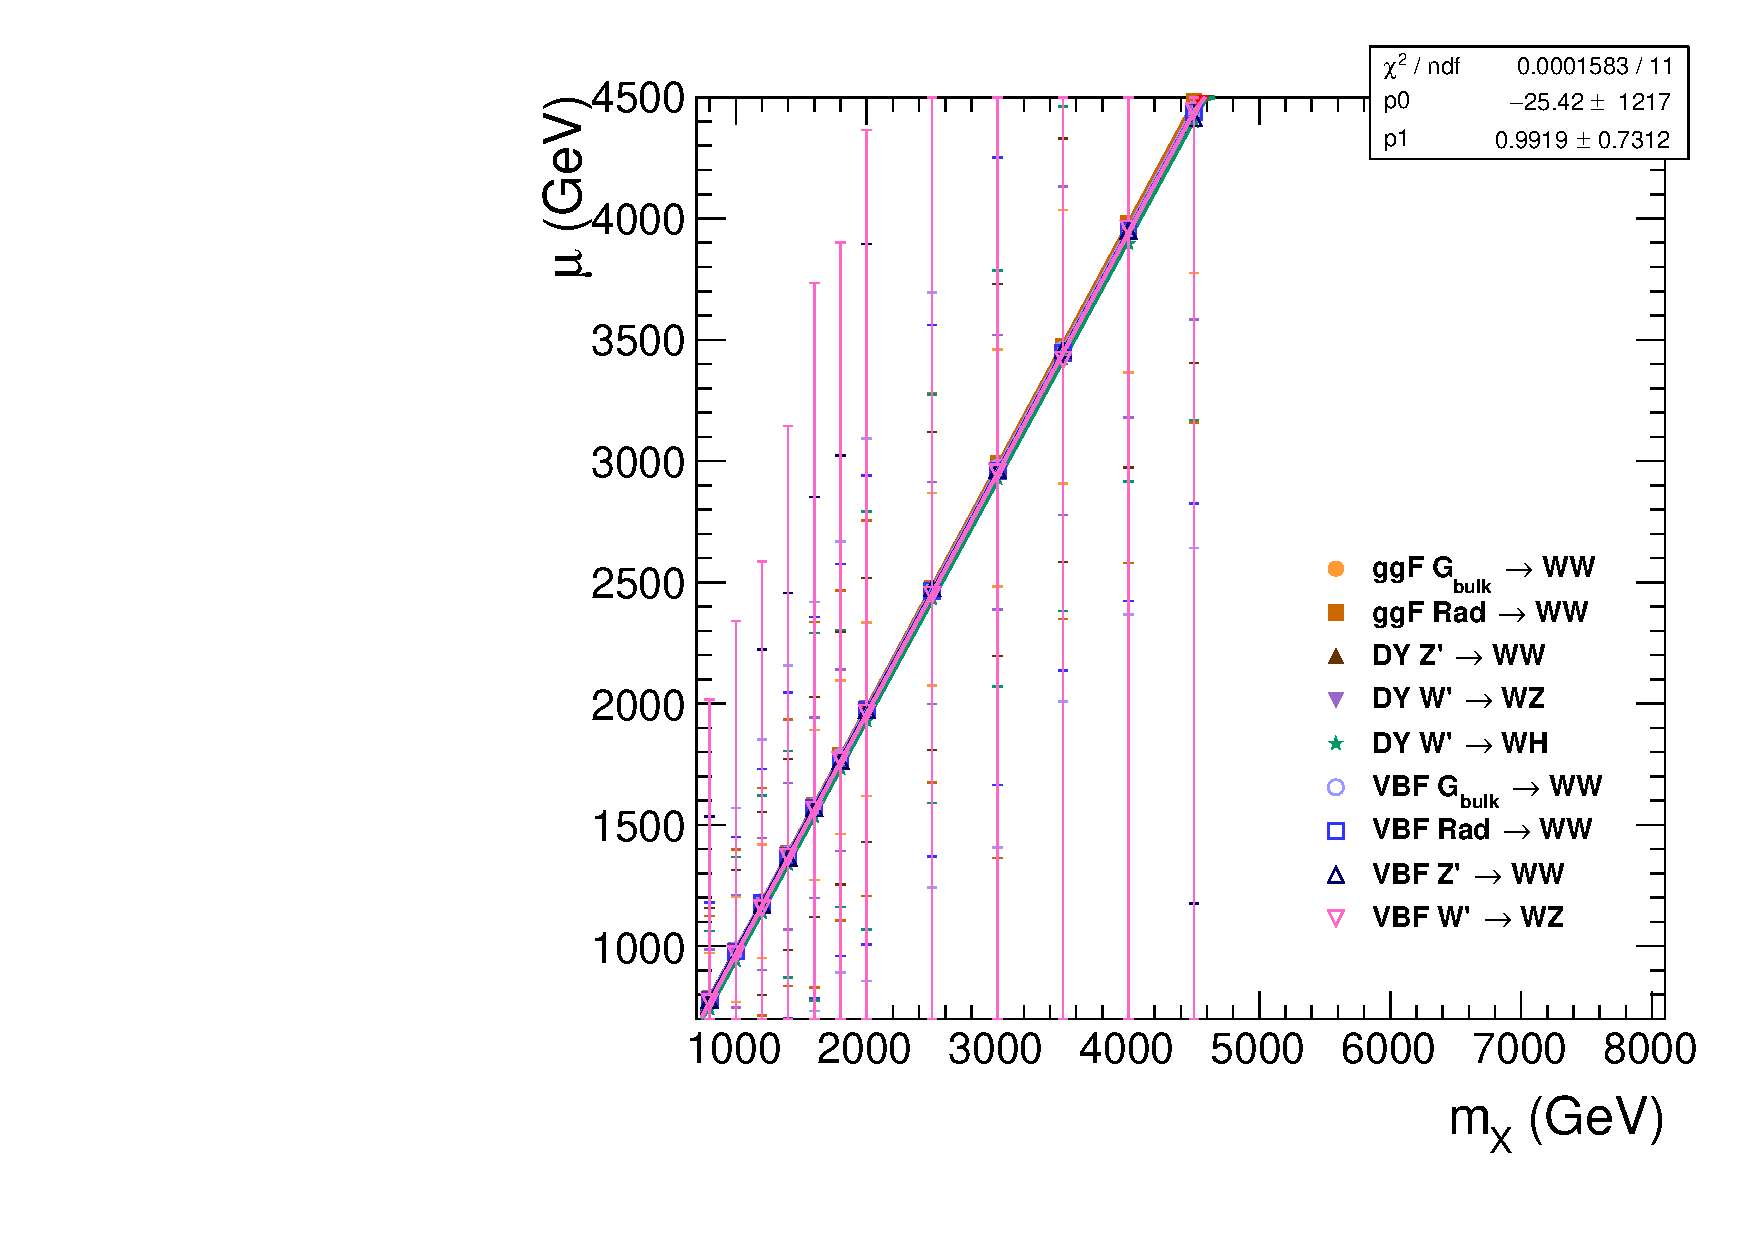
\includegraphics[width=0.2\textwidth]{fig/2Dfit/paramSignalShape_allSig_MVV_LP_nobb_LDy_MEAN.pdf}
  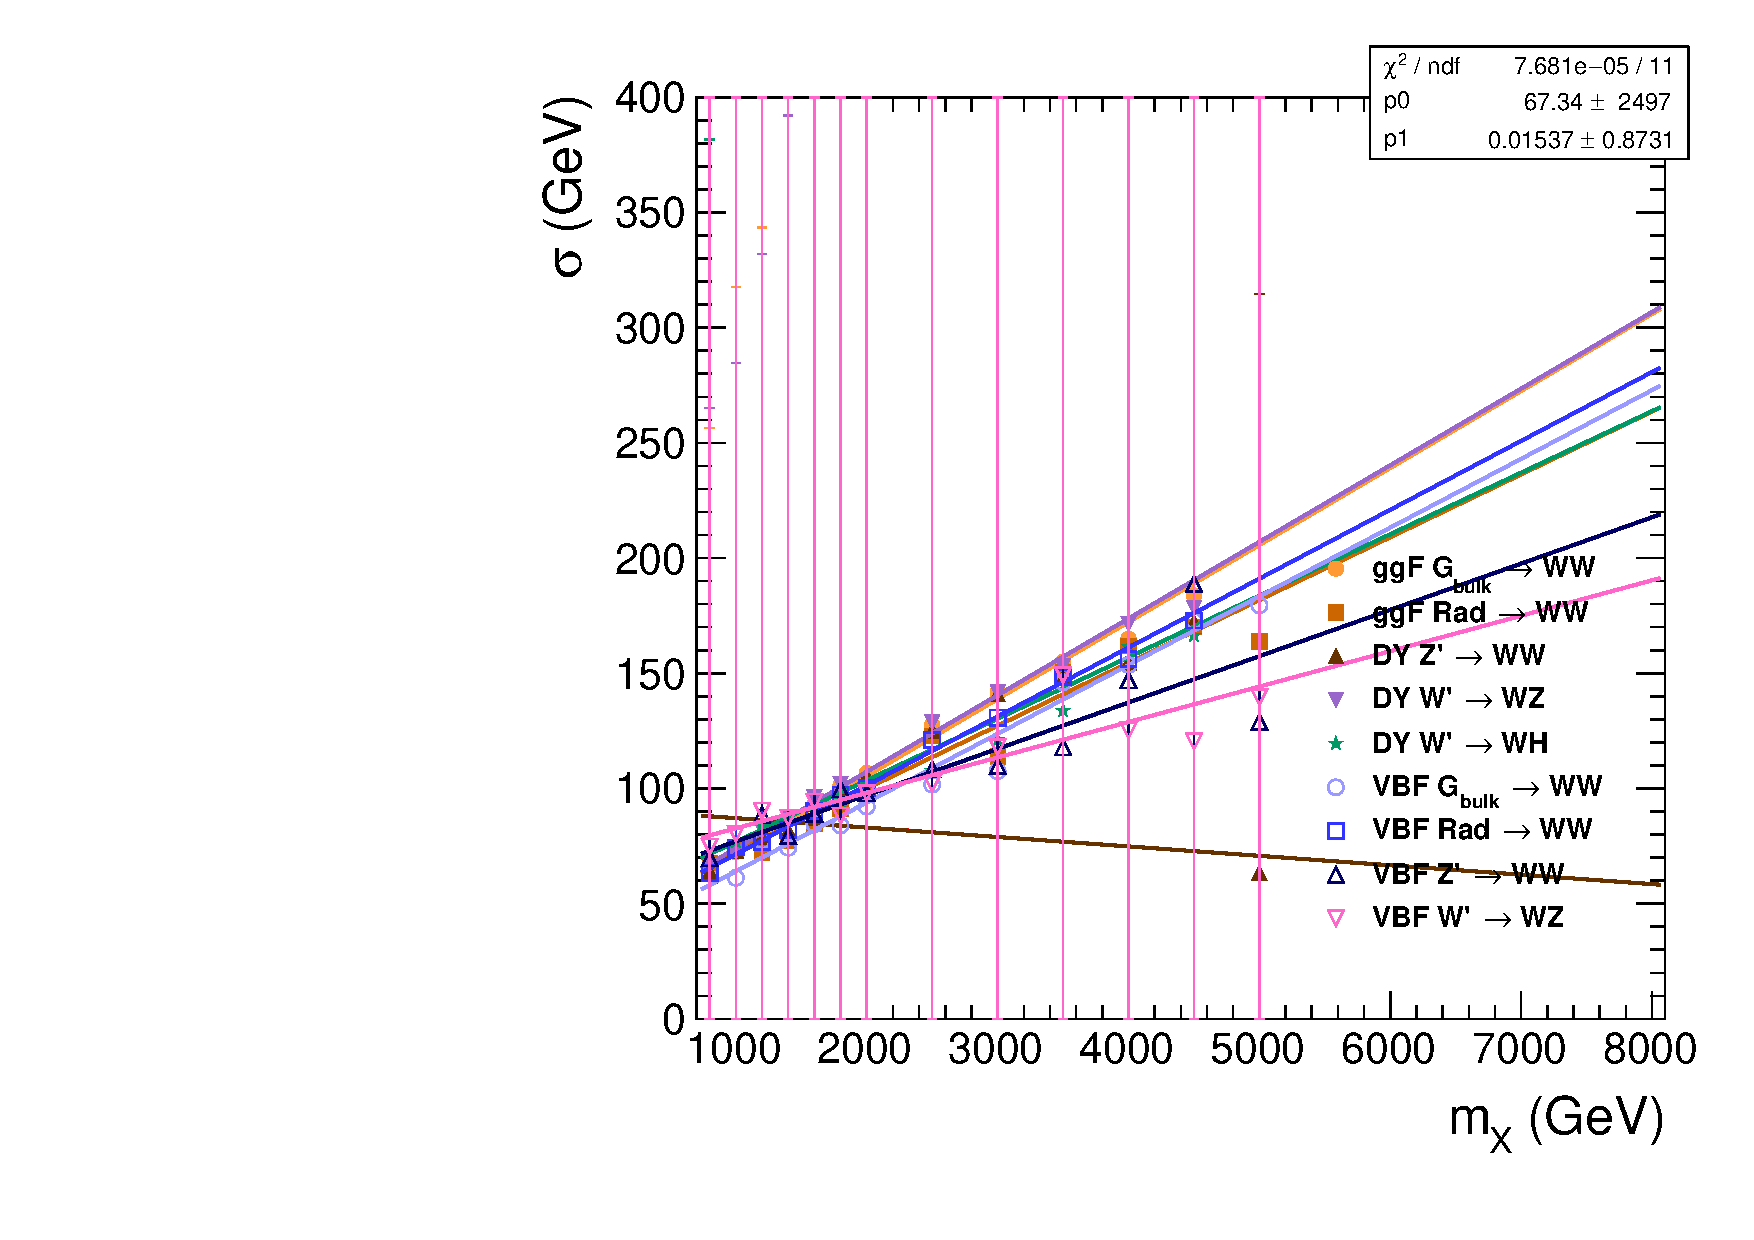
\includegraphics[width=0.2\textwidth]{fig/2Dfit/paramSignalShape_allSig_MVV_LP_nobb_LDy_SIGMA.pdf}
  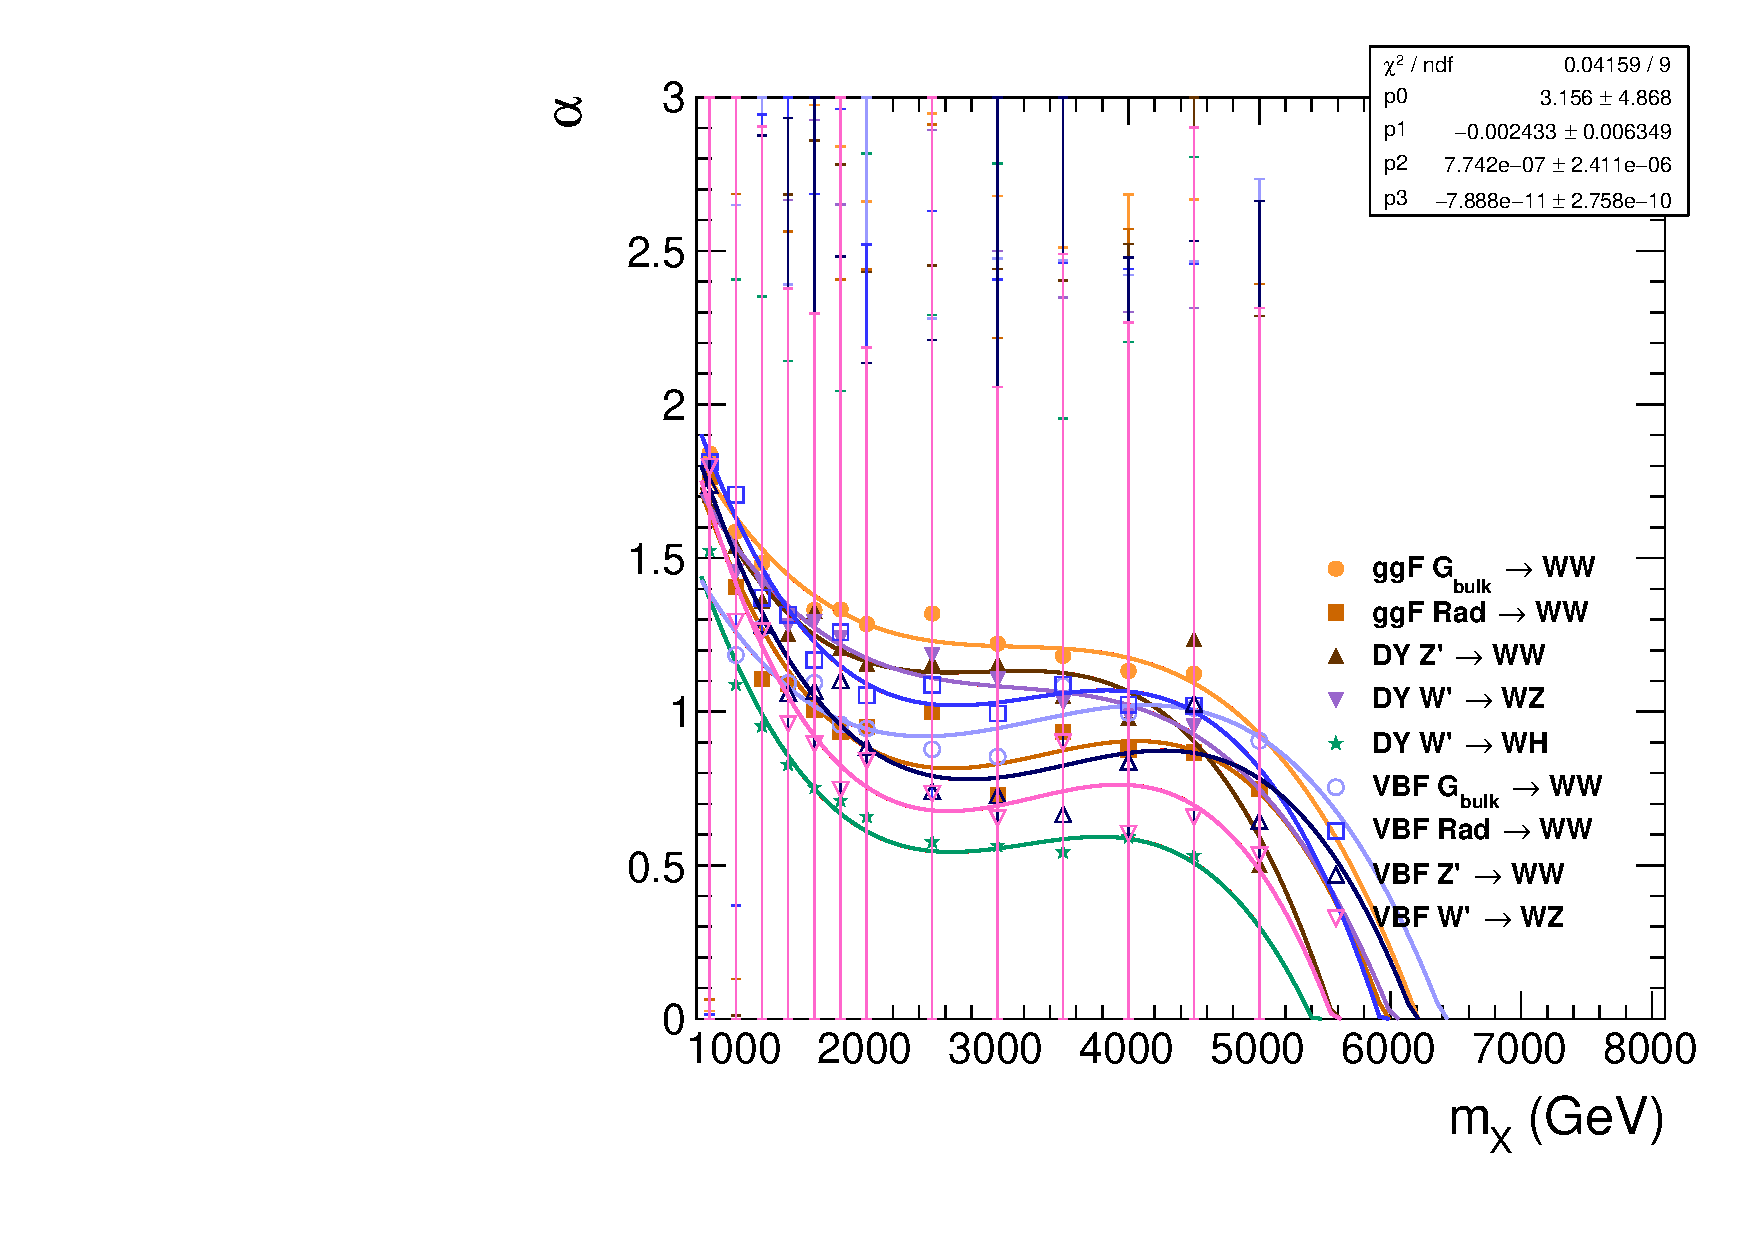
\includegraphics[width=0.2\textwidth]{fig/2Dfit/paramSignalShape_allSig_MVV_LP_nobb_LDy_ALPHA1.pdf}
  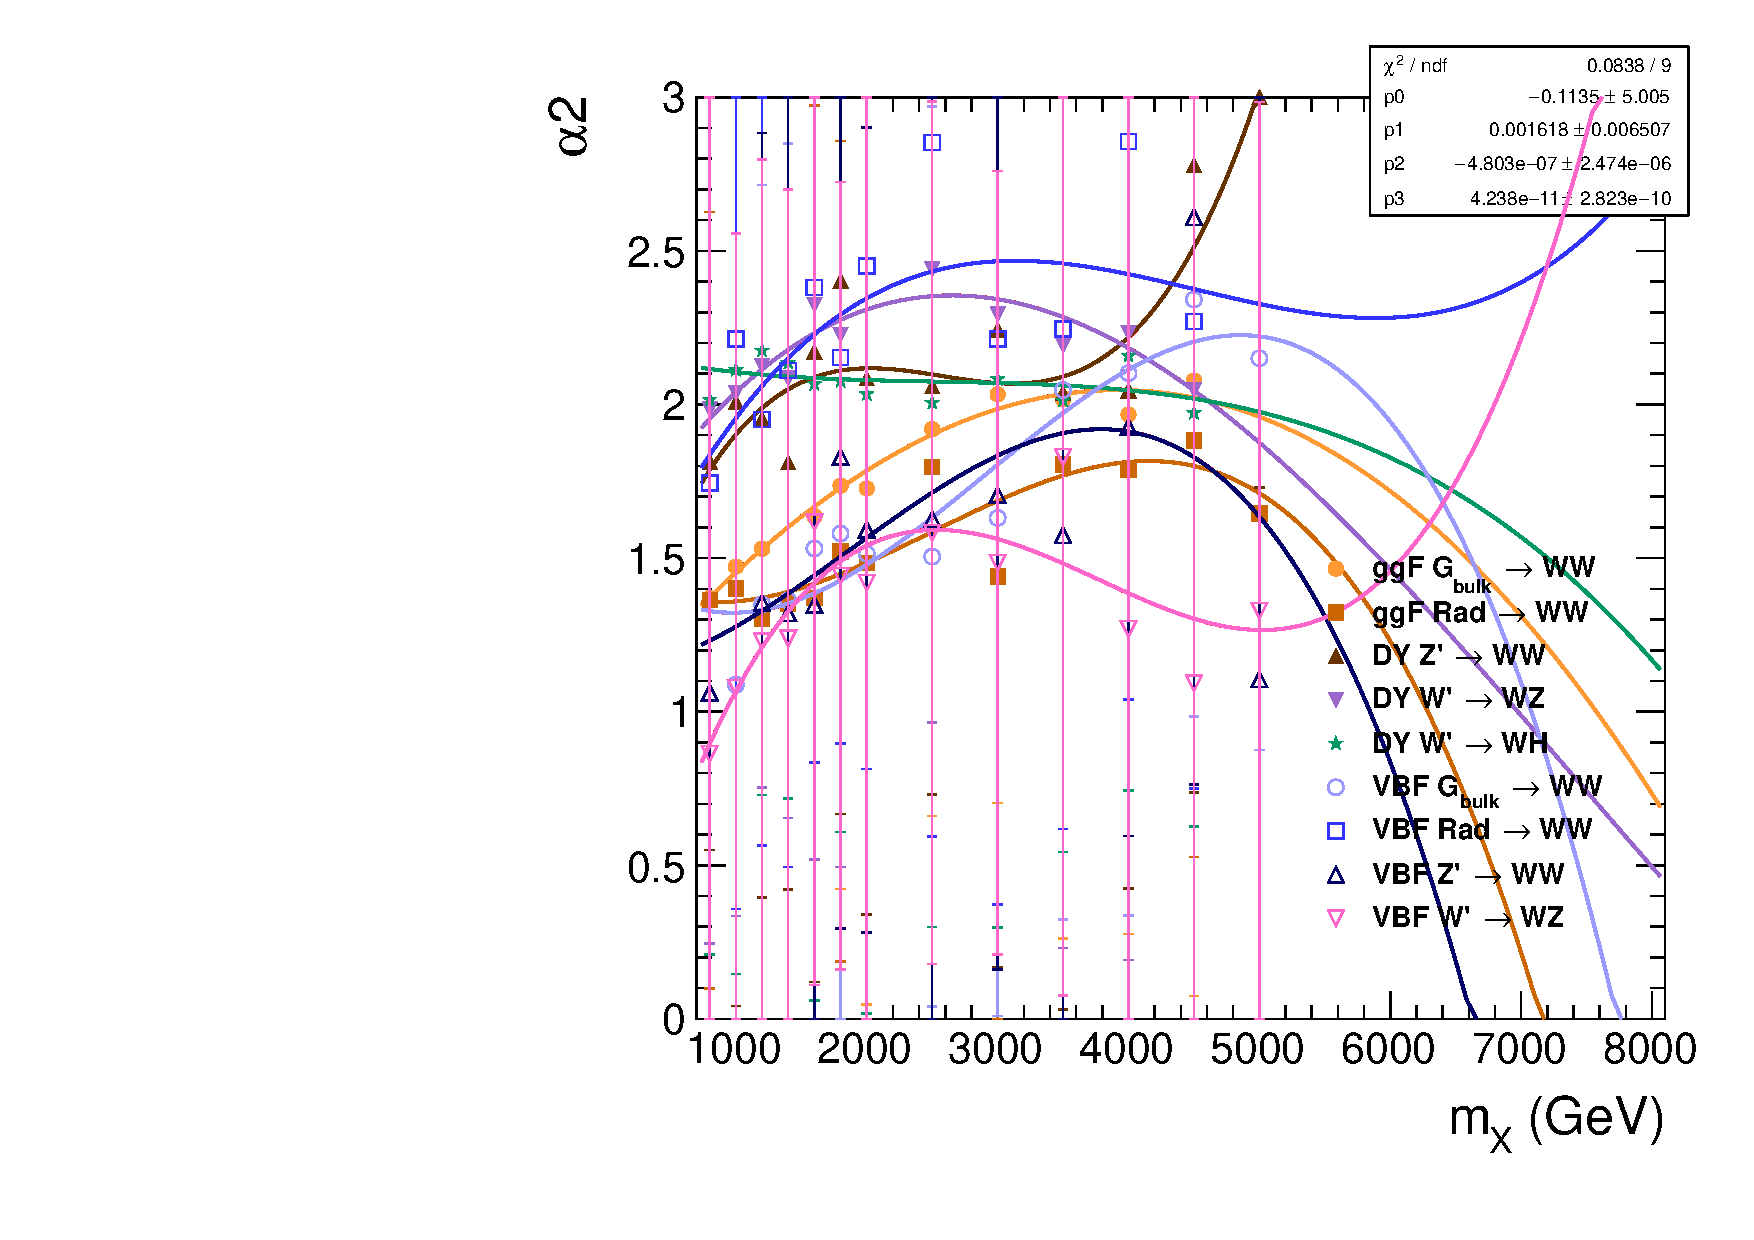
\includegraphics[width=0.2\textwidth]{fig/2Dfit/paramSignalShape_allSig_MVV_LP_nobb_LDy_ALPHA2.pdf}\\
  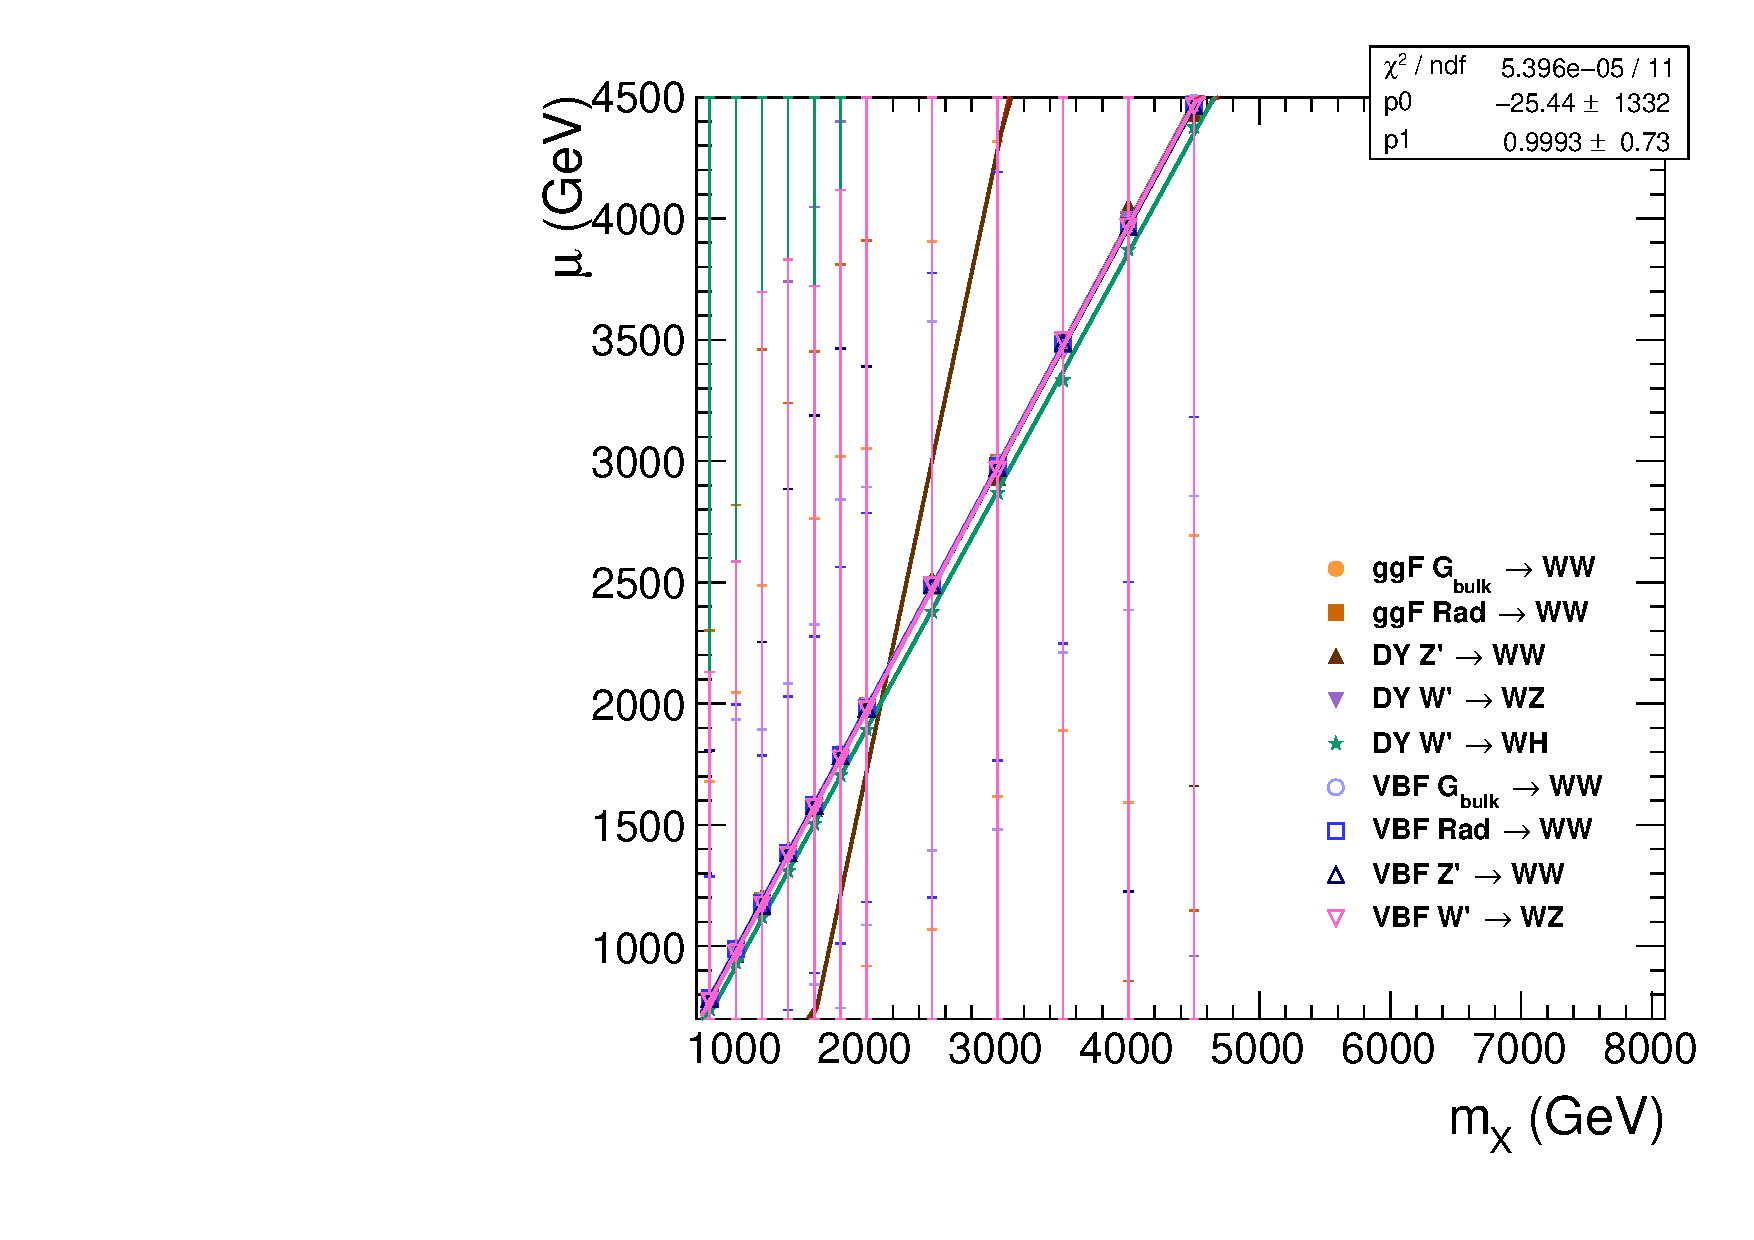
\includegraphics[width=0.2\textwidth]{fig/2Dfit/paramSignalShape_allSig_MVV_HP_vbf_LDy_MEAN.pdf}
  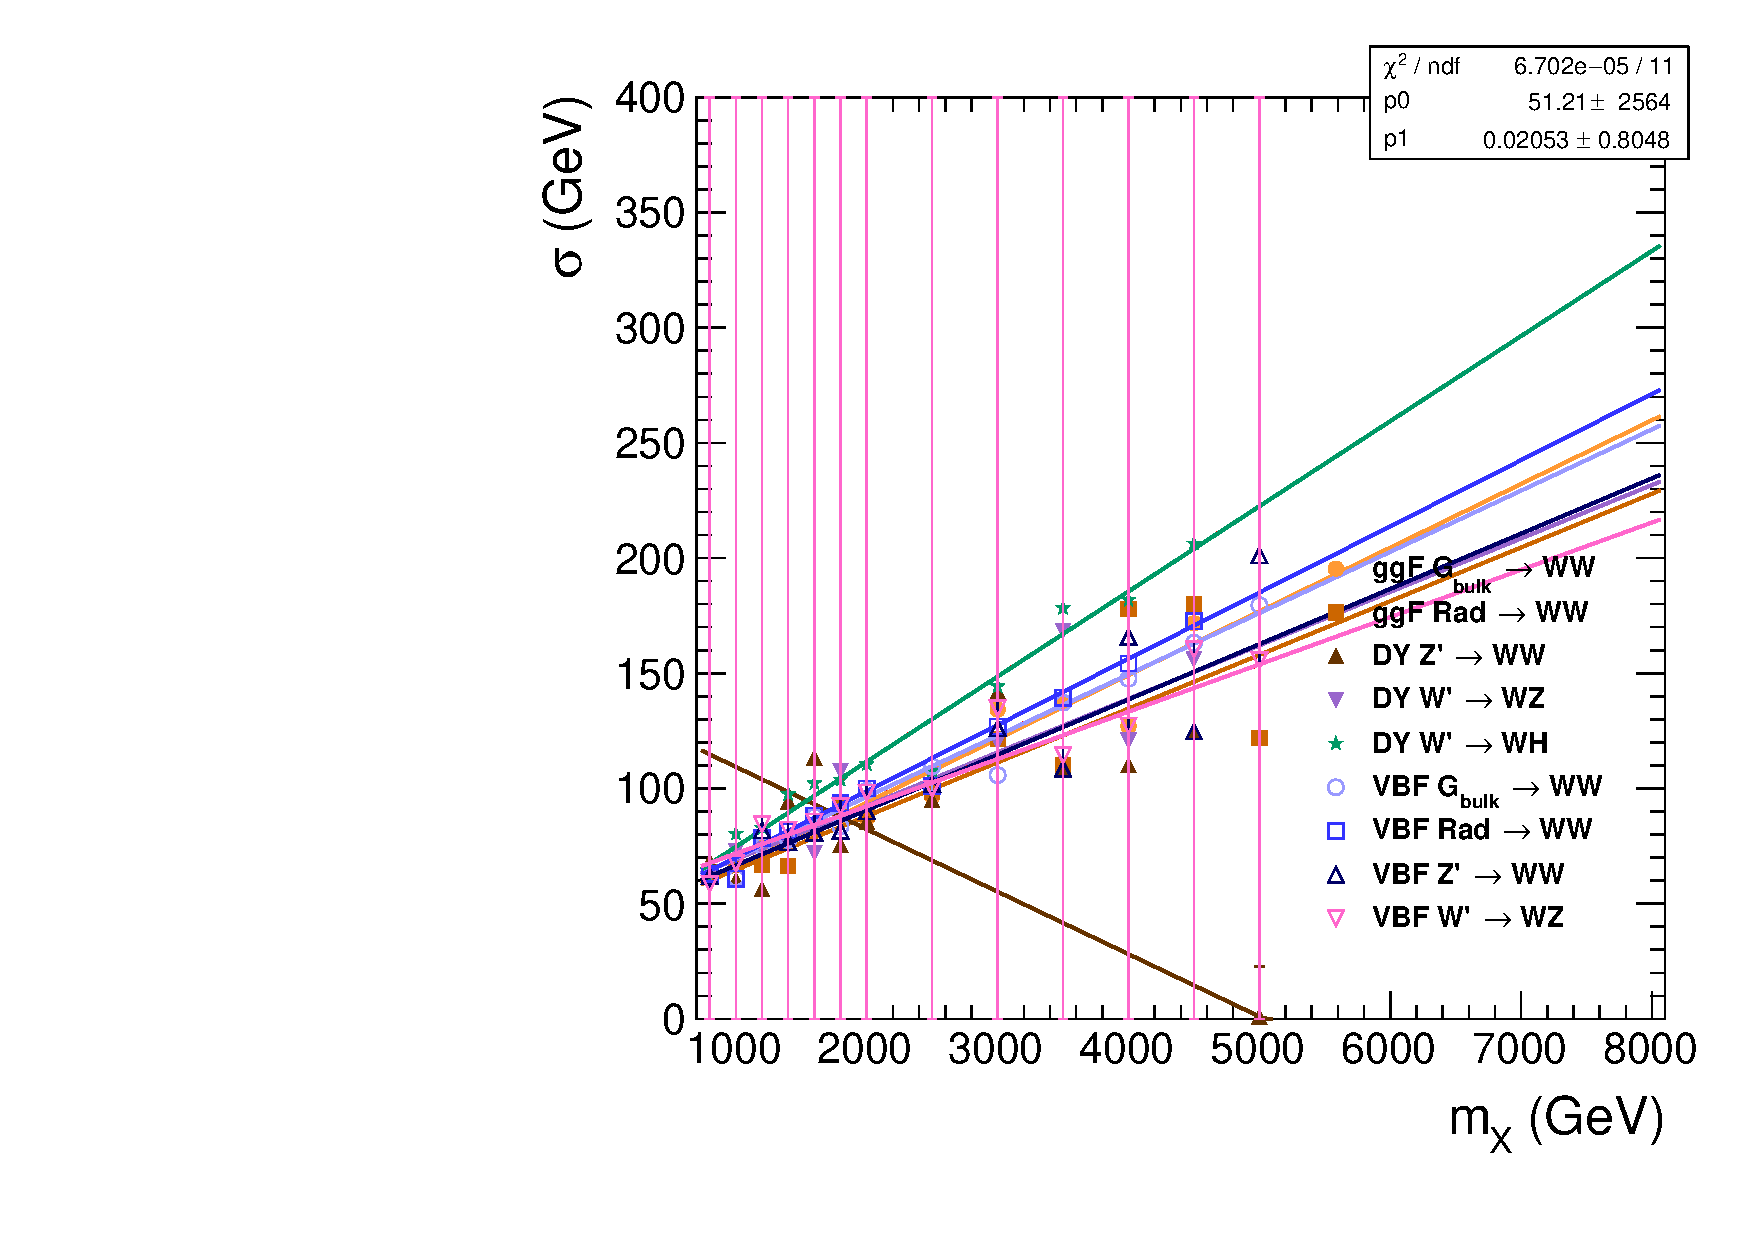
\includegraphics[width=0.2\textwidth]{fig/2Dfit/paramSignalShape_allSig_MVV_HP_vbf_LDy_SIGMA.pdf}
  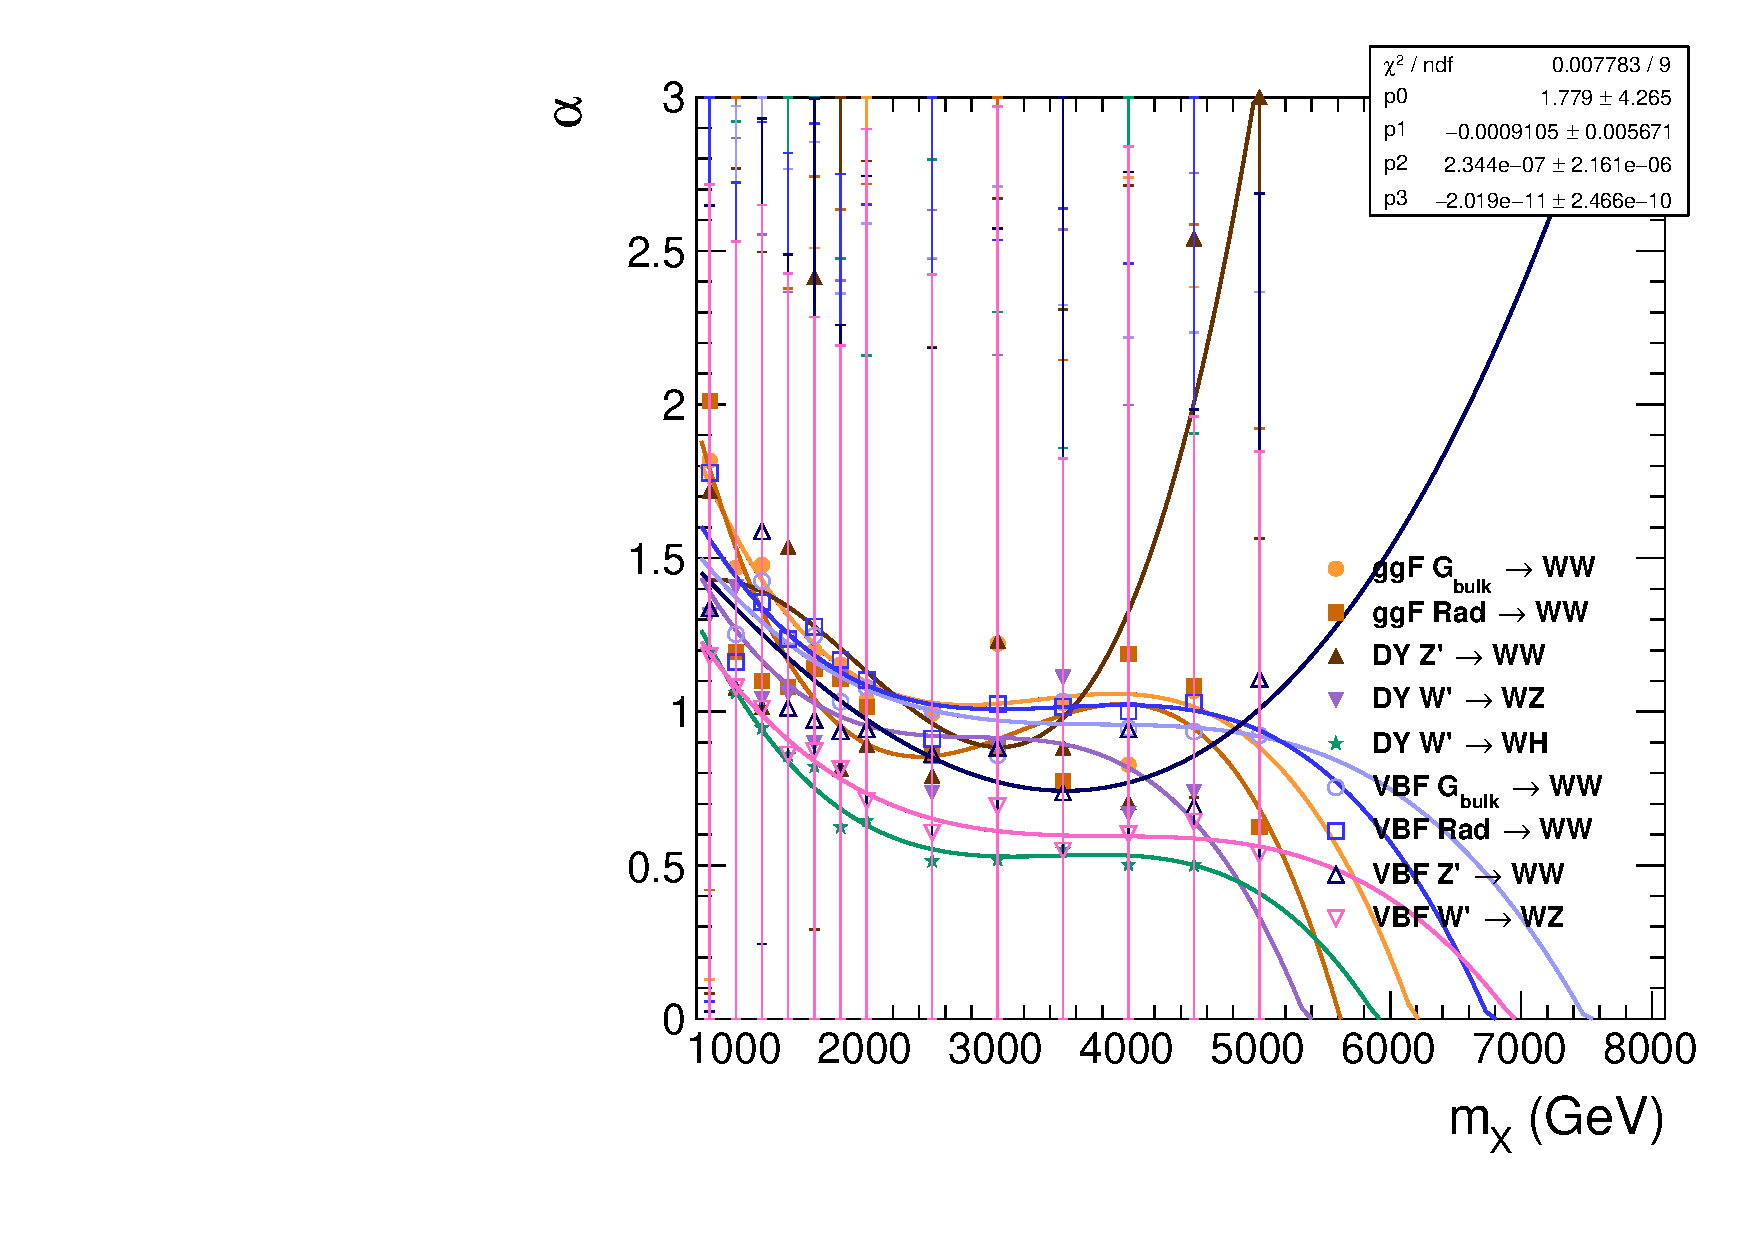
\includegraphics[width=0.2\textwidth]{fig/2Dfit/paramSignalShape_allSig_MVV_HP_vbf_LDy_ALPHA1.pdf}
  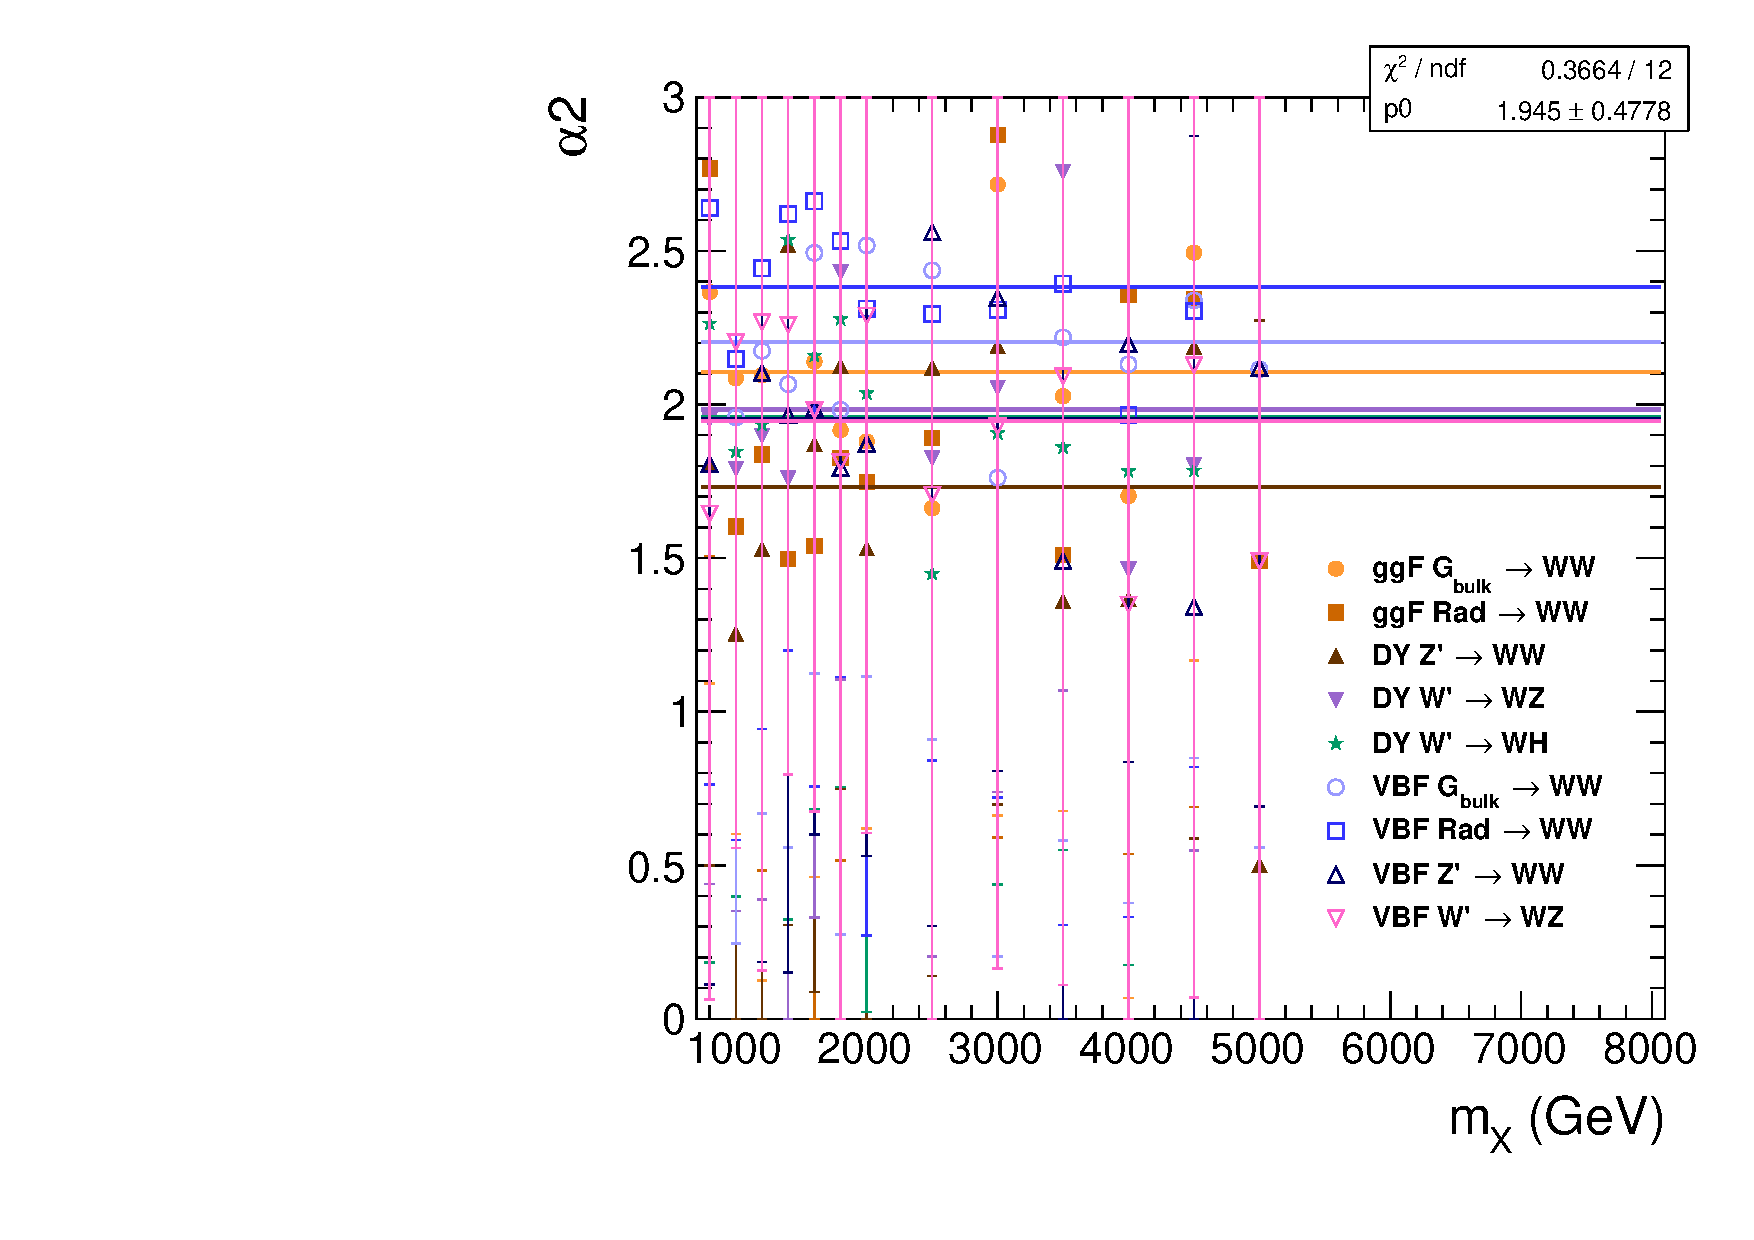
\includegraphics[width=0.2\textwidth]{fig/2Dfit/paramSignalShape_allSig_MVV_HP_vbf_LDy_ALPHA2.pdf}\\
  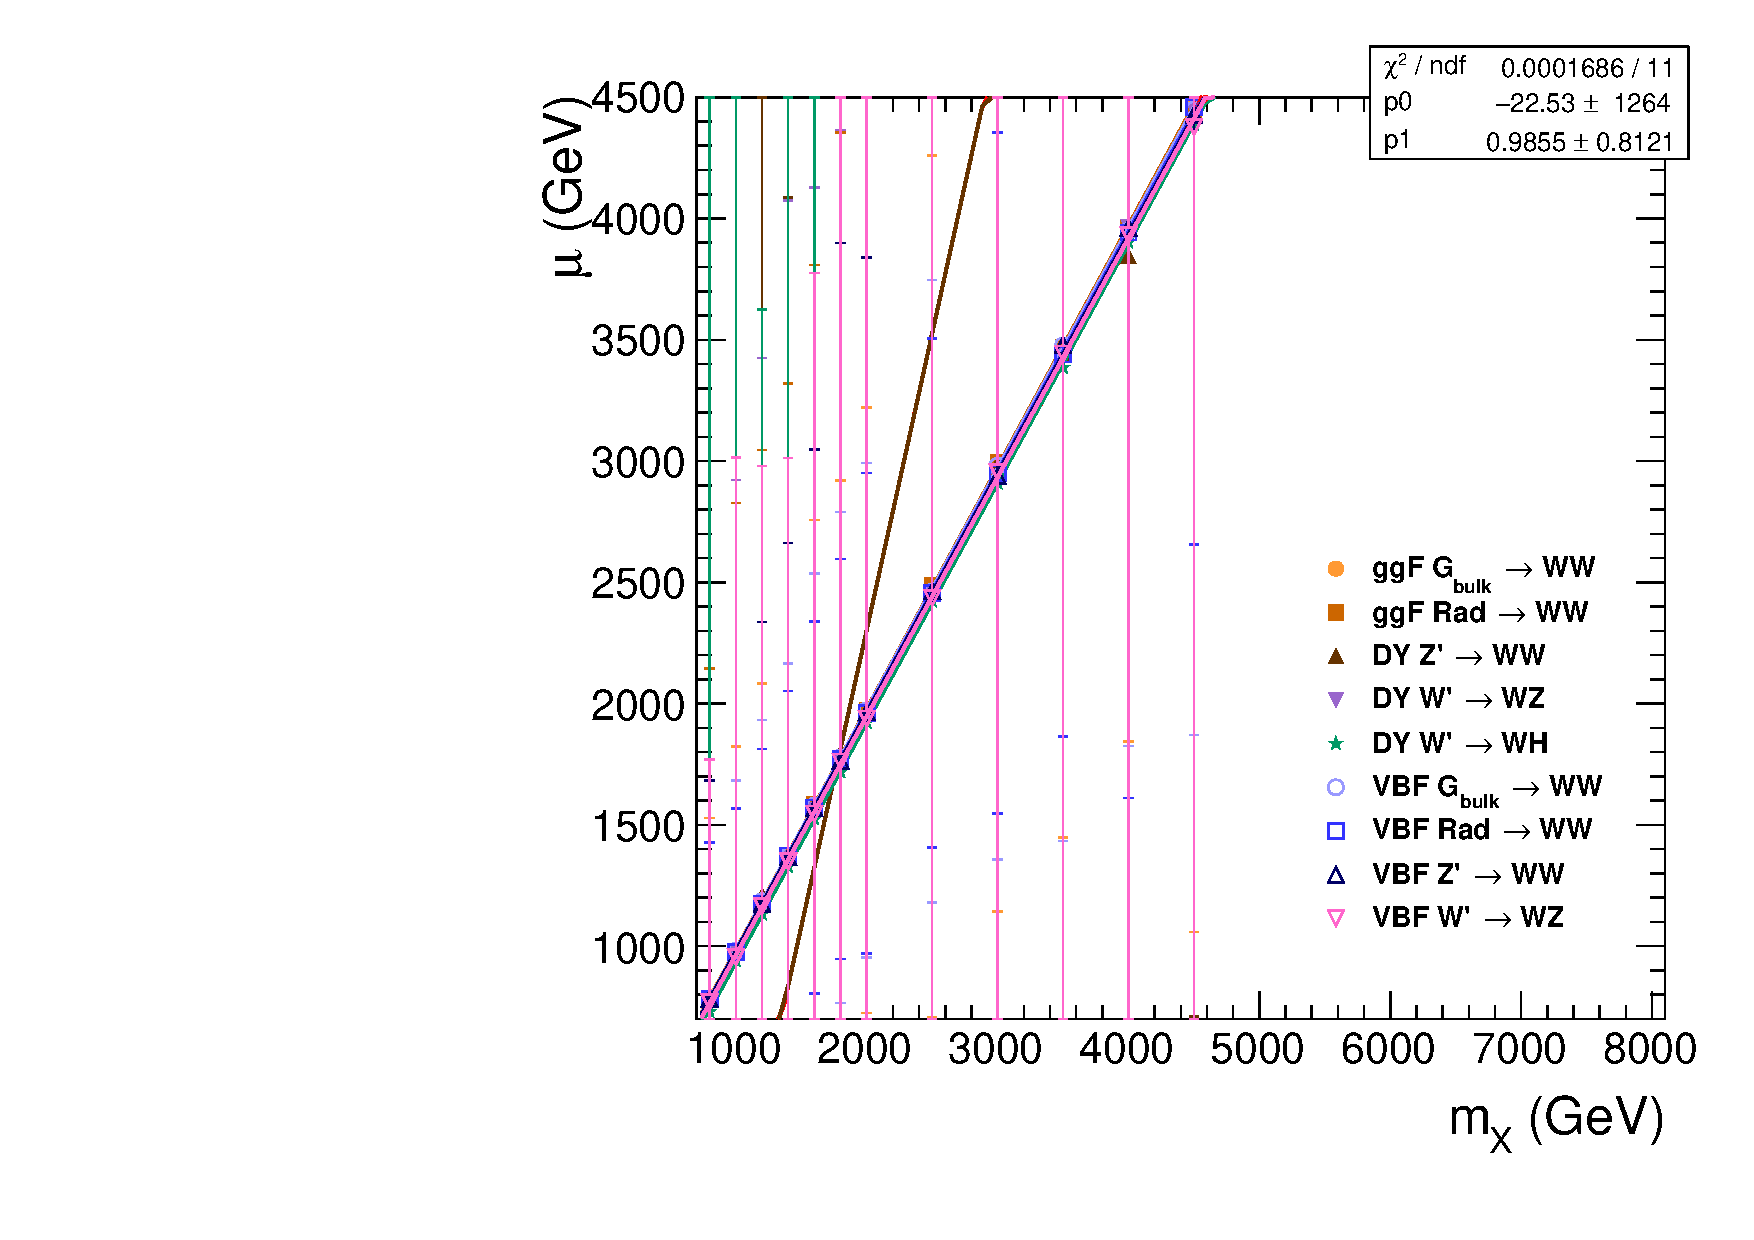
\includegraphics[width=0.2\textwidth]{fig/2Dfit/paramSignalShape_allSig_MVV_LP_vbf_LDy_MEAN.pdf}
  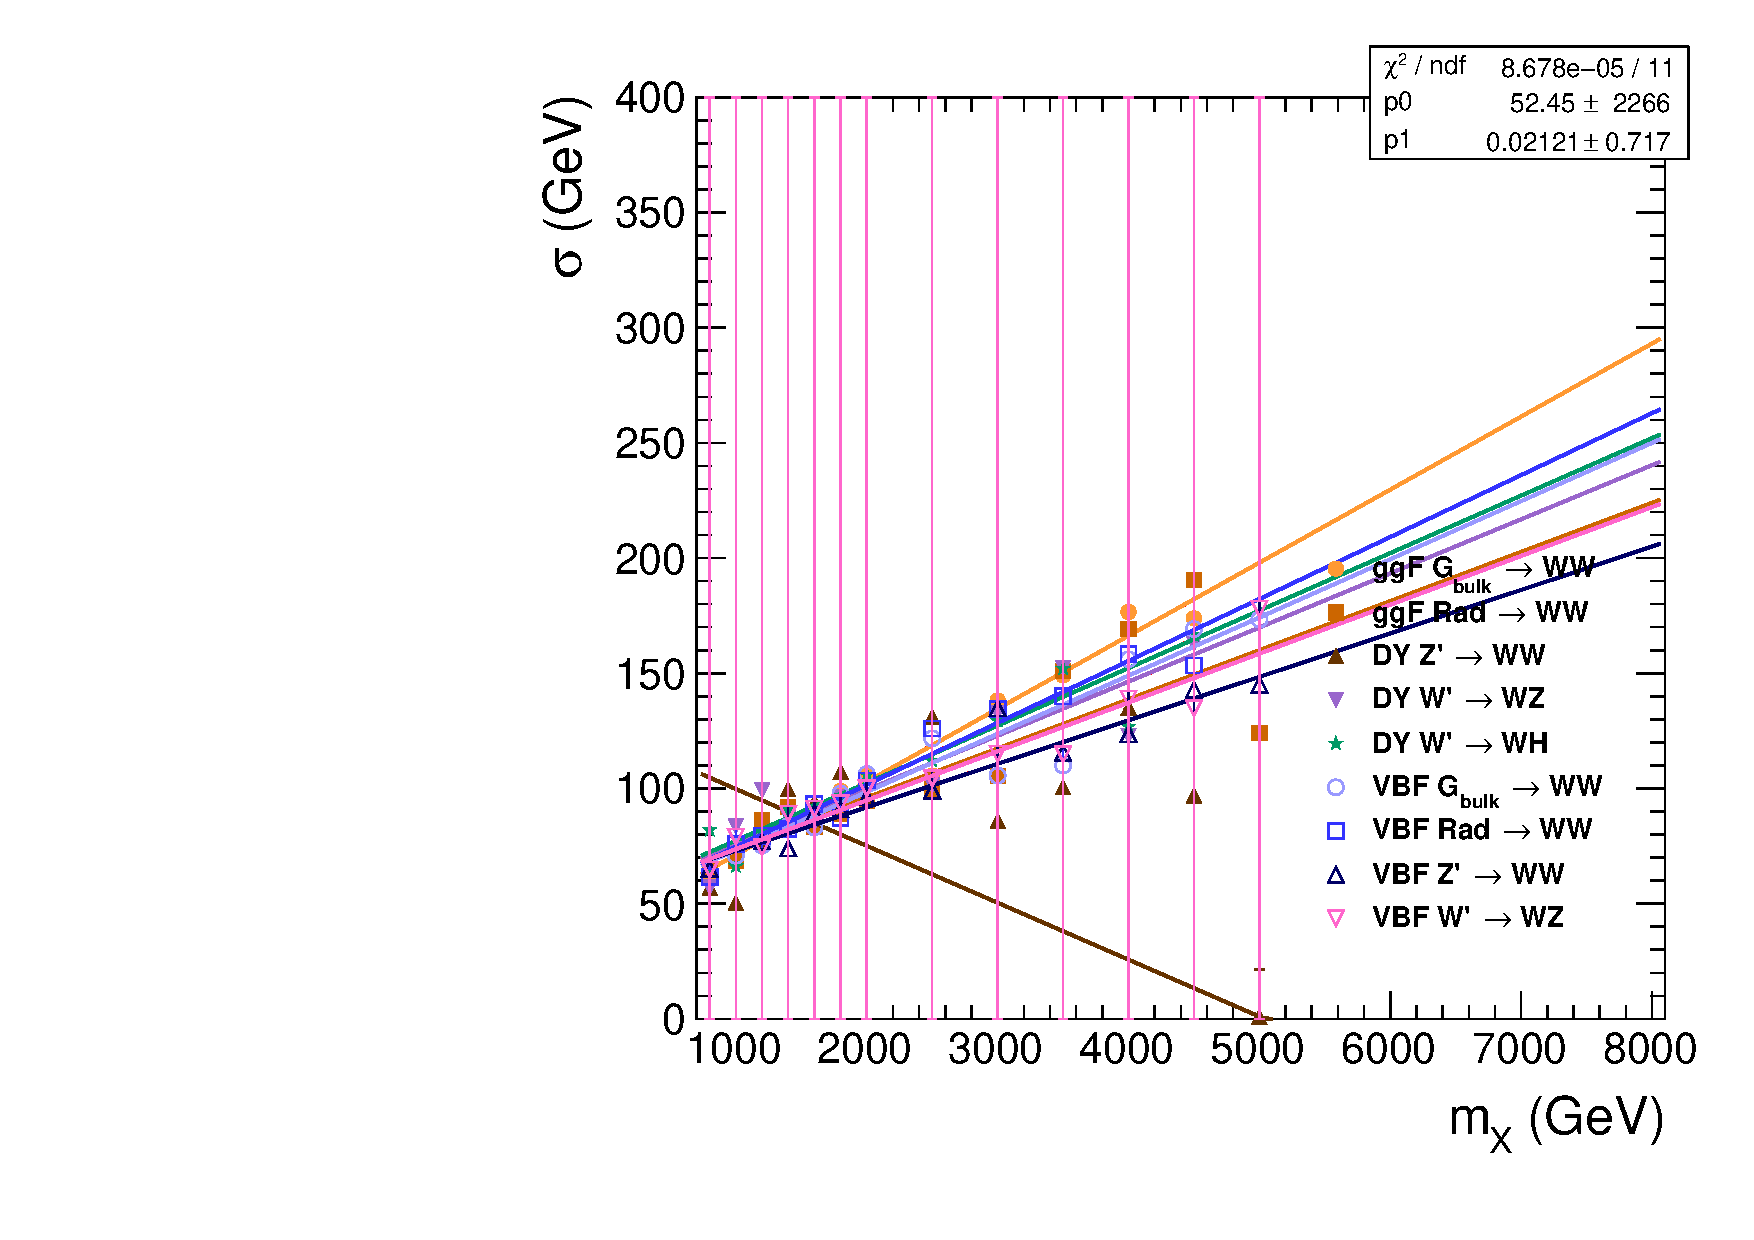
\includegraphics[width=0.2\textwidth]{fig/2Dfit/paramSignalShape_allSig_MVV_LP_vbf_LDy_SIGMA.pdf}
  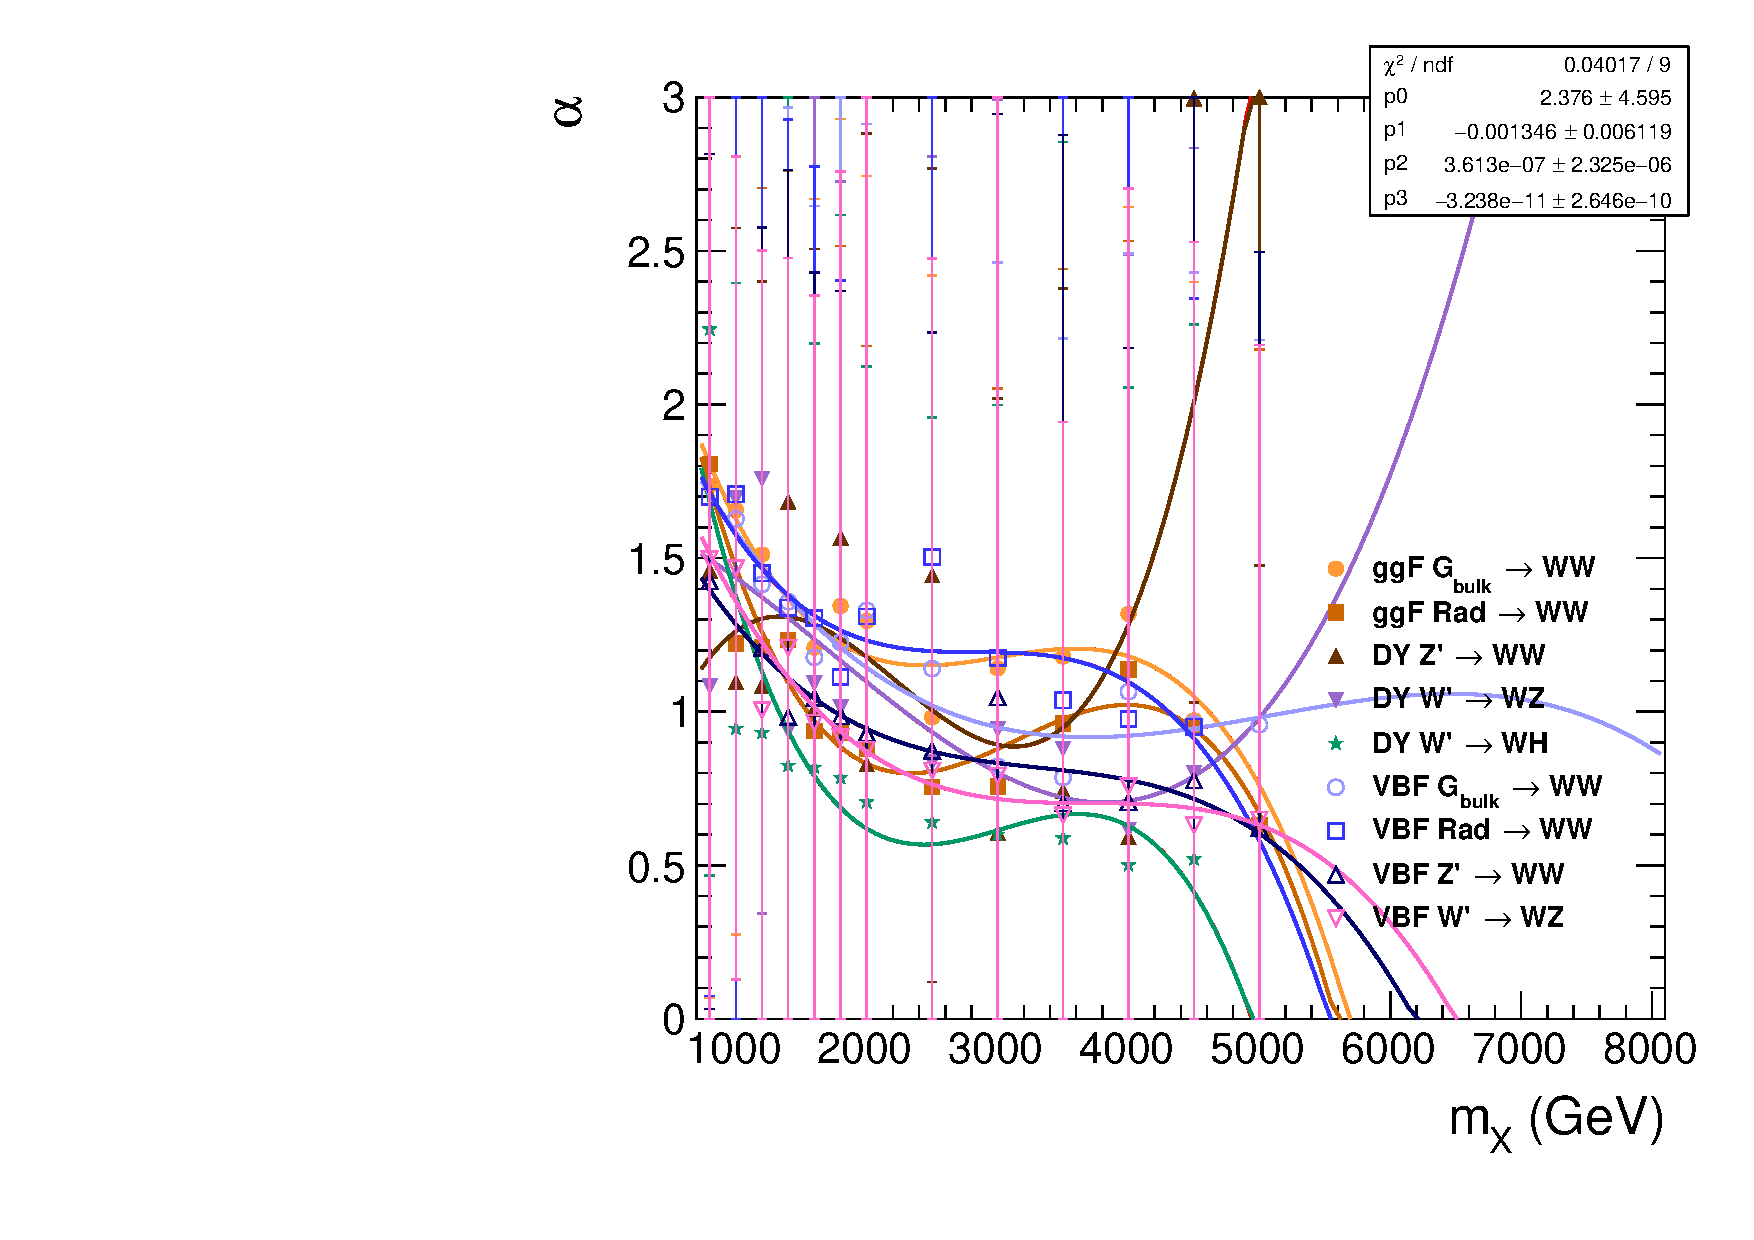
\includegraphics[width=0.2\textwidth]{fig/2Dfit/paramSignalShape_allSig_MVV_LP_vbf_LDy_ALPHA1.pdf}
  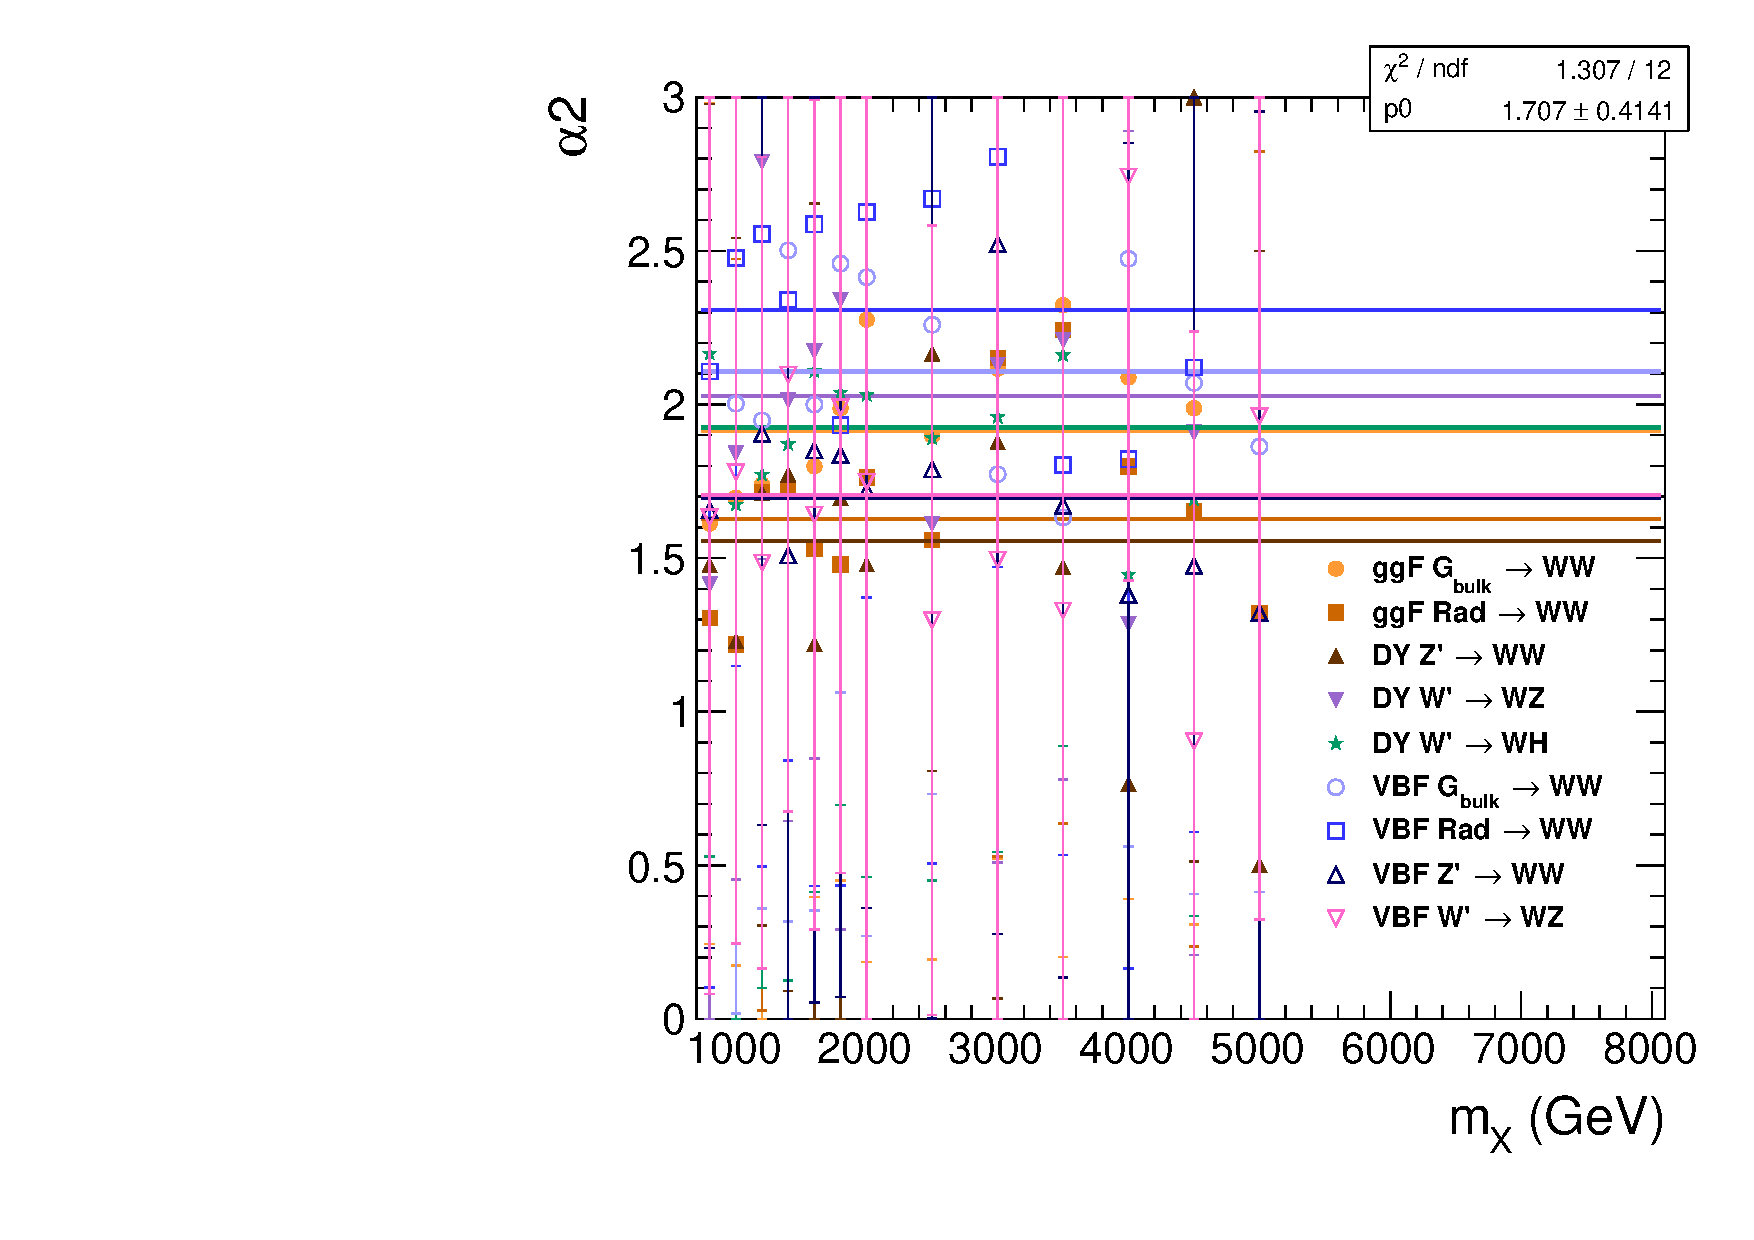
\includegraphics[width=0.2\textwidth]{fig/2Dfit/paramSignalShape_allSig_MVV_LP_vbf_LDy_ALPHA2.pdf}\\
  \caption{
    DCB parameters (from left to right: $\mu$, $\sigma$, $\alpha_1$, $\alpha_2$) for the diboson reconstructed mass \MVV as a function of \MX.
    Rows 1 to 6: HP-bb-LDy, LP-bb-LDy, HP-nobb-LDy, LP-nobb-LDy, HP-vbf-LDy, LP-vbf-LDy.
  }
  \label{fig:MVVShapeParam_LDy_Run2}
\end{figure}

\begin{figure}[htbp]
  \centering
  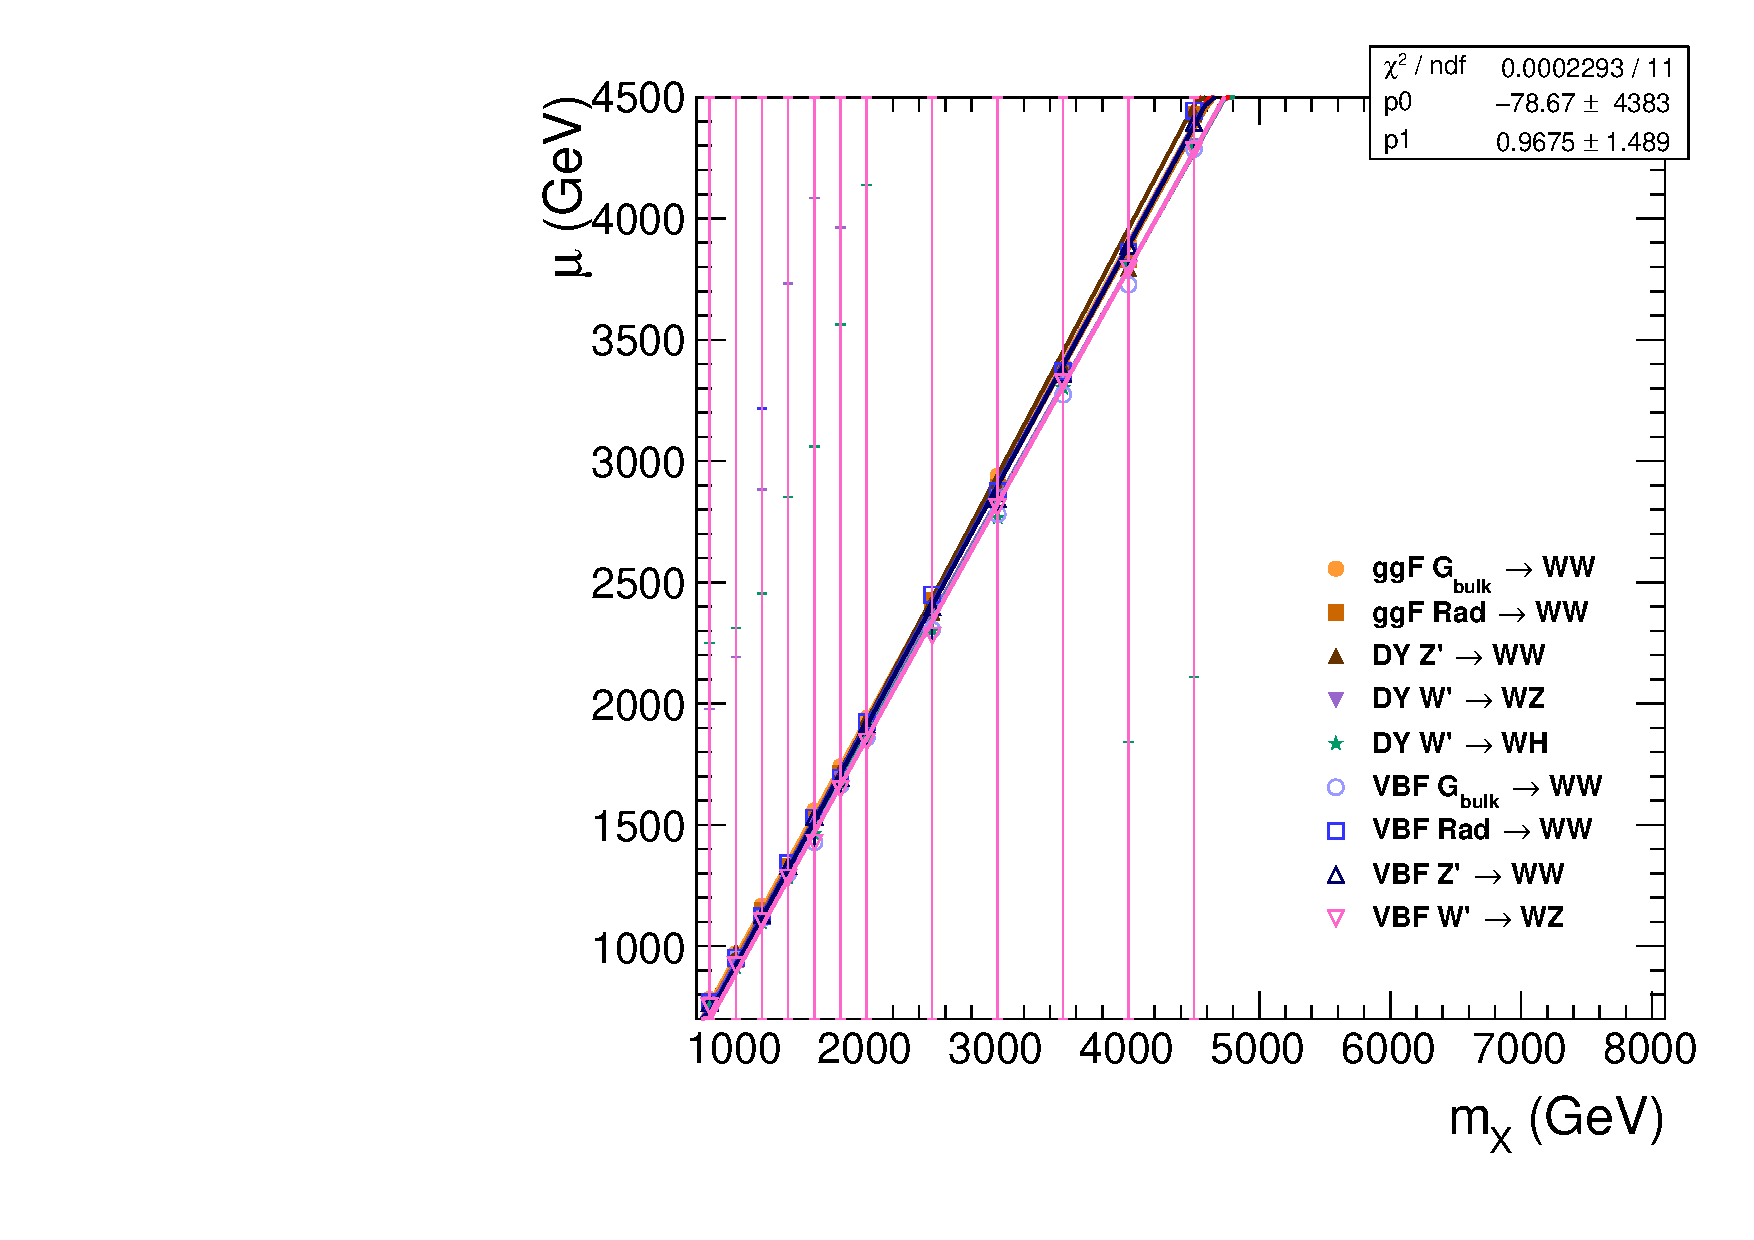
\includegraphics[width=0.2\textwidth]{fig/2Dfit/paramSignalShape_allSig_MVV_HP_bb_HDy_MEAN.pdf}
  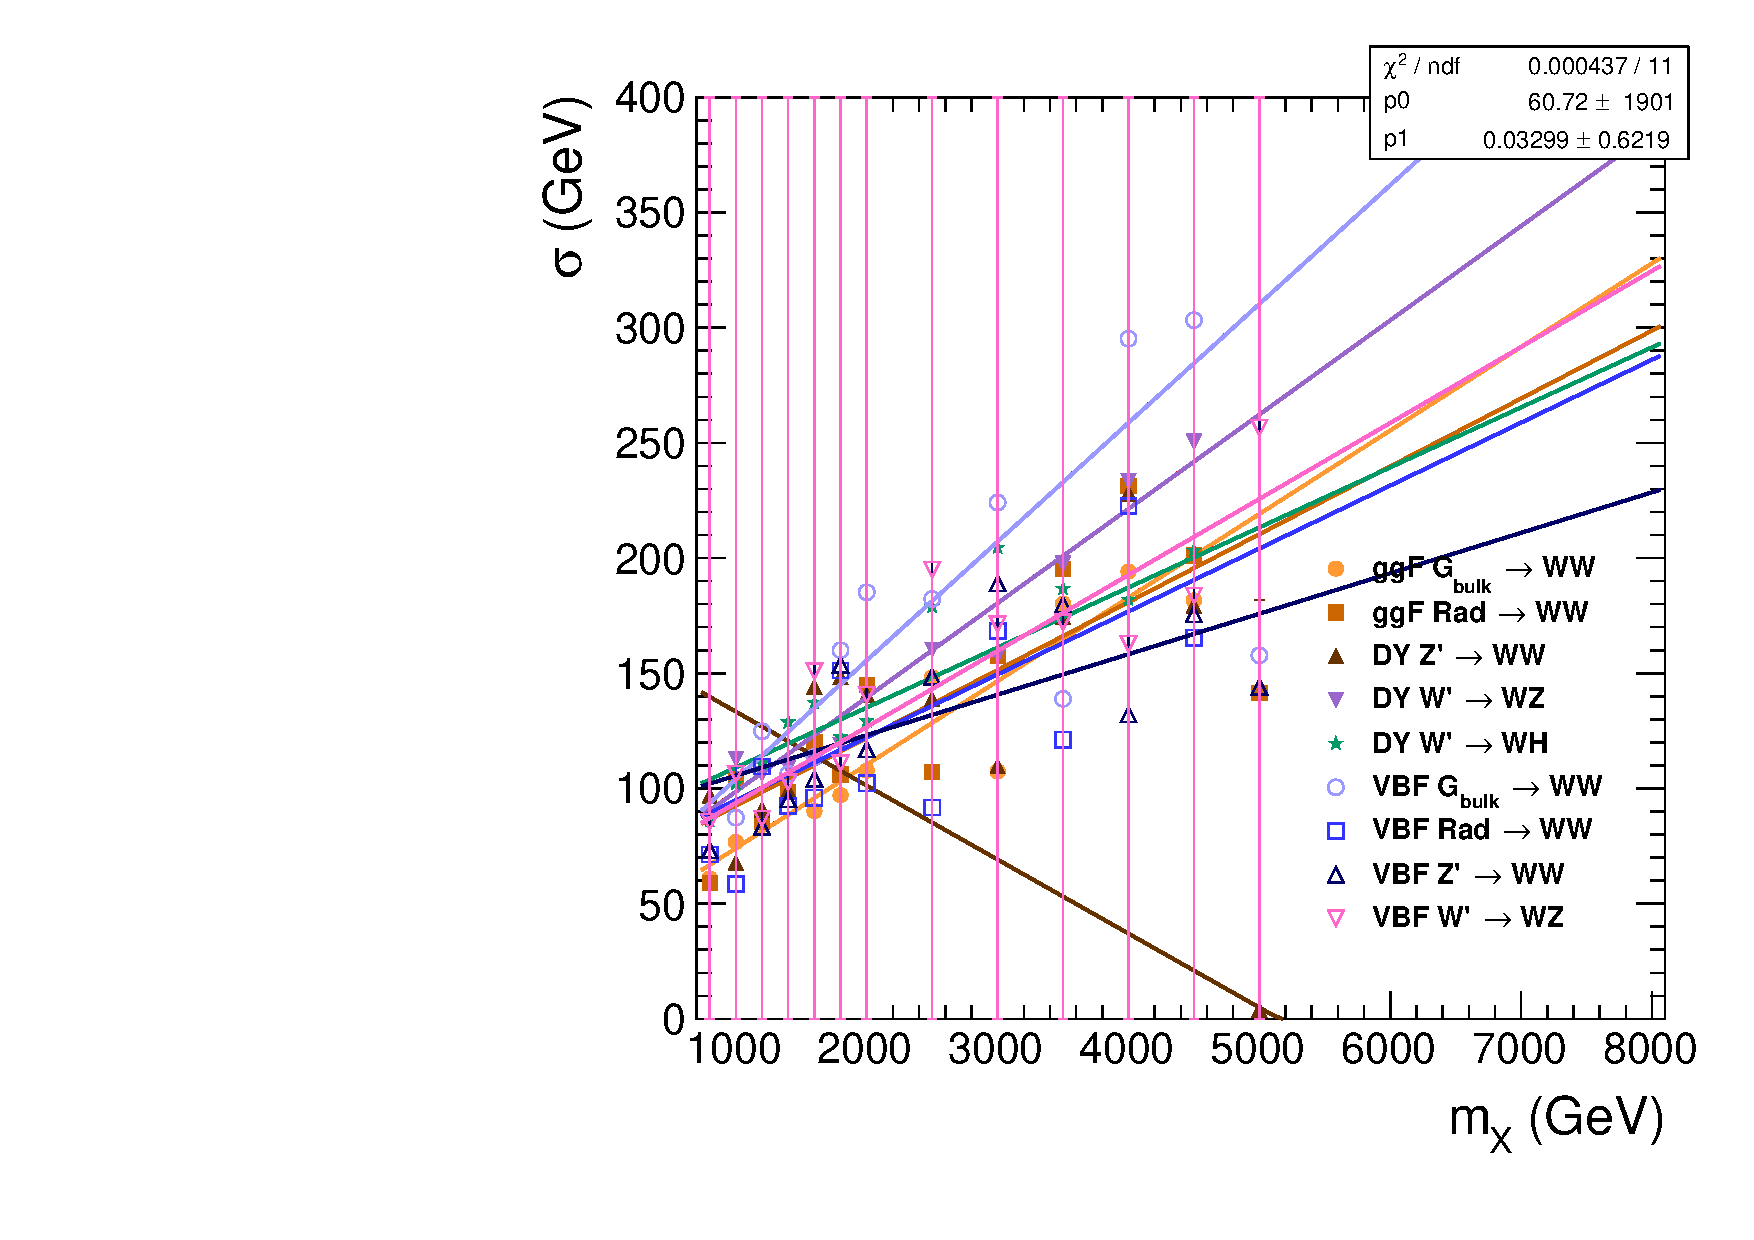
\includegraphics[width=0.2\textwidth]{fig/2Dfit/paramSignalShape_allSig_MVV_HP_bb_HDy_SIGMA.pdf}
  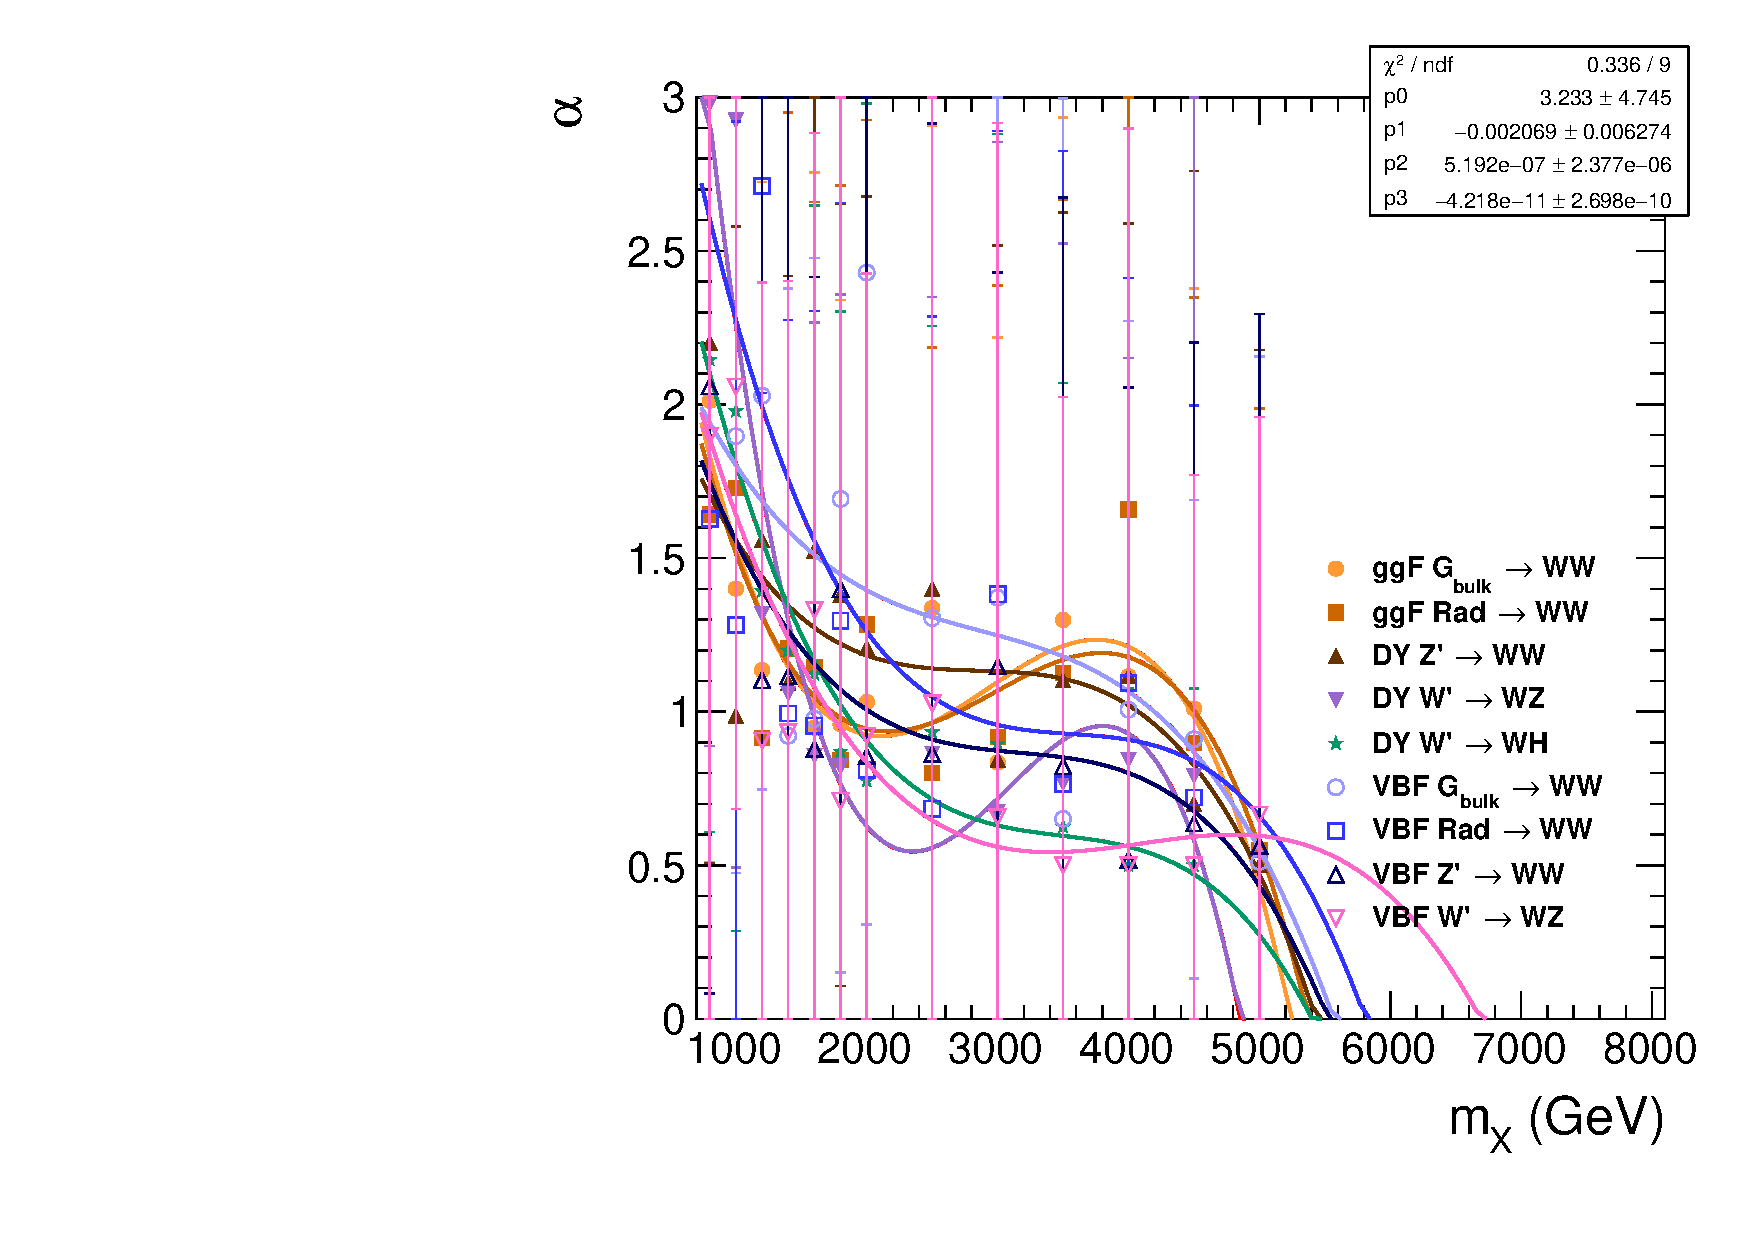
\includegraphics[width=0.2\textwidth]{fig/2Dfit/paramSignalShape_allSig_MVV_HP_bb_HDy_ALPHA1.pdf}
  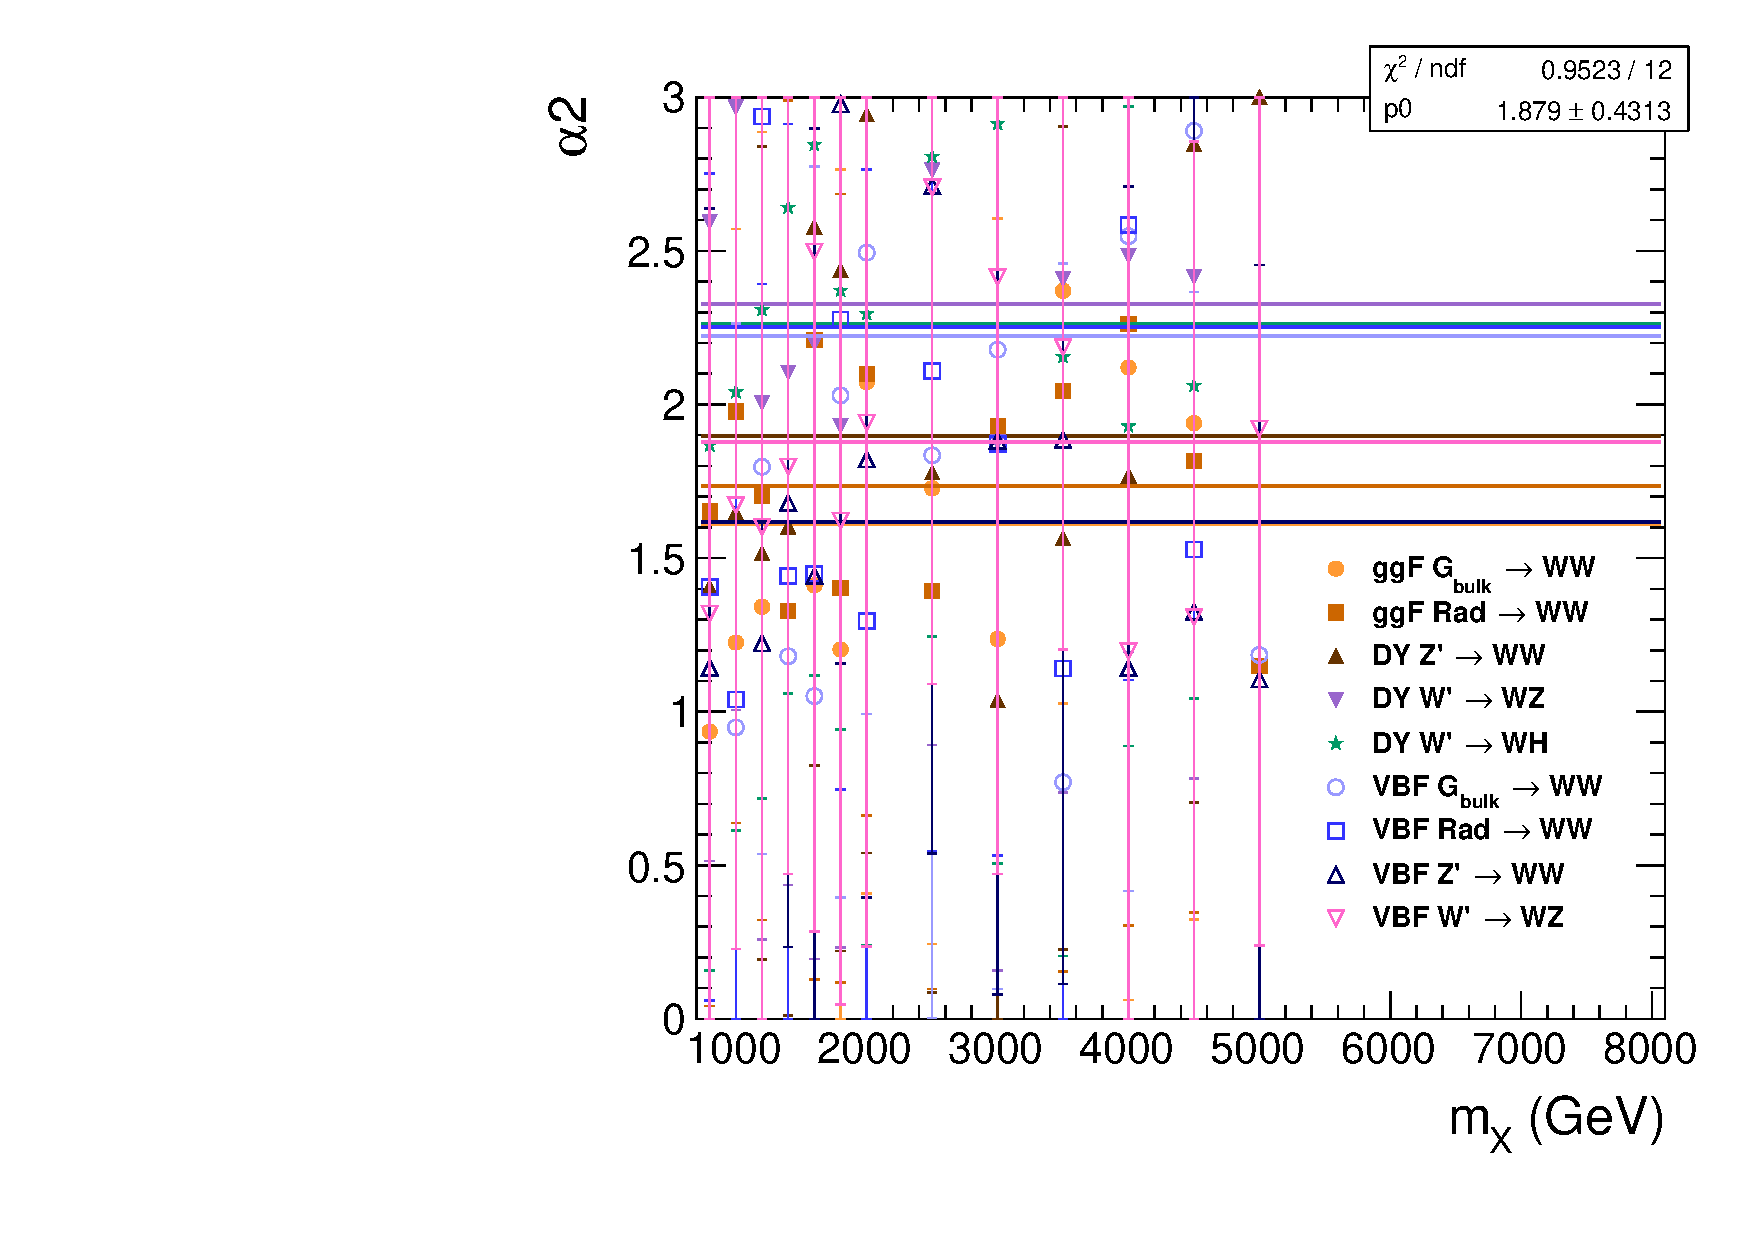
\includegraphics[width=0.2\textwidth]{fig/2Dfit/paramSignalShape_allSig_MVV_HP_bb_HDy_ALPHA2.pdf}\\
  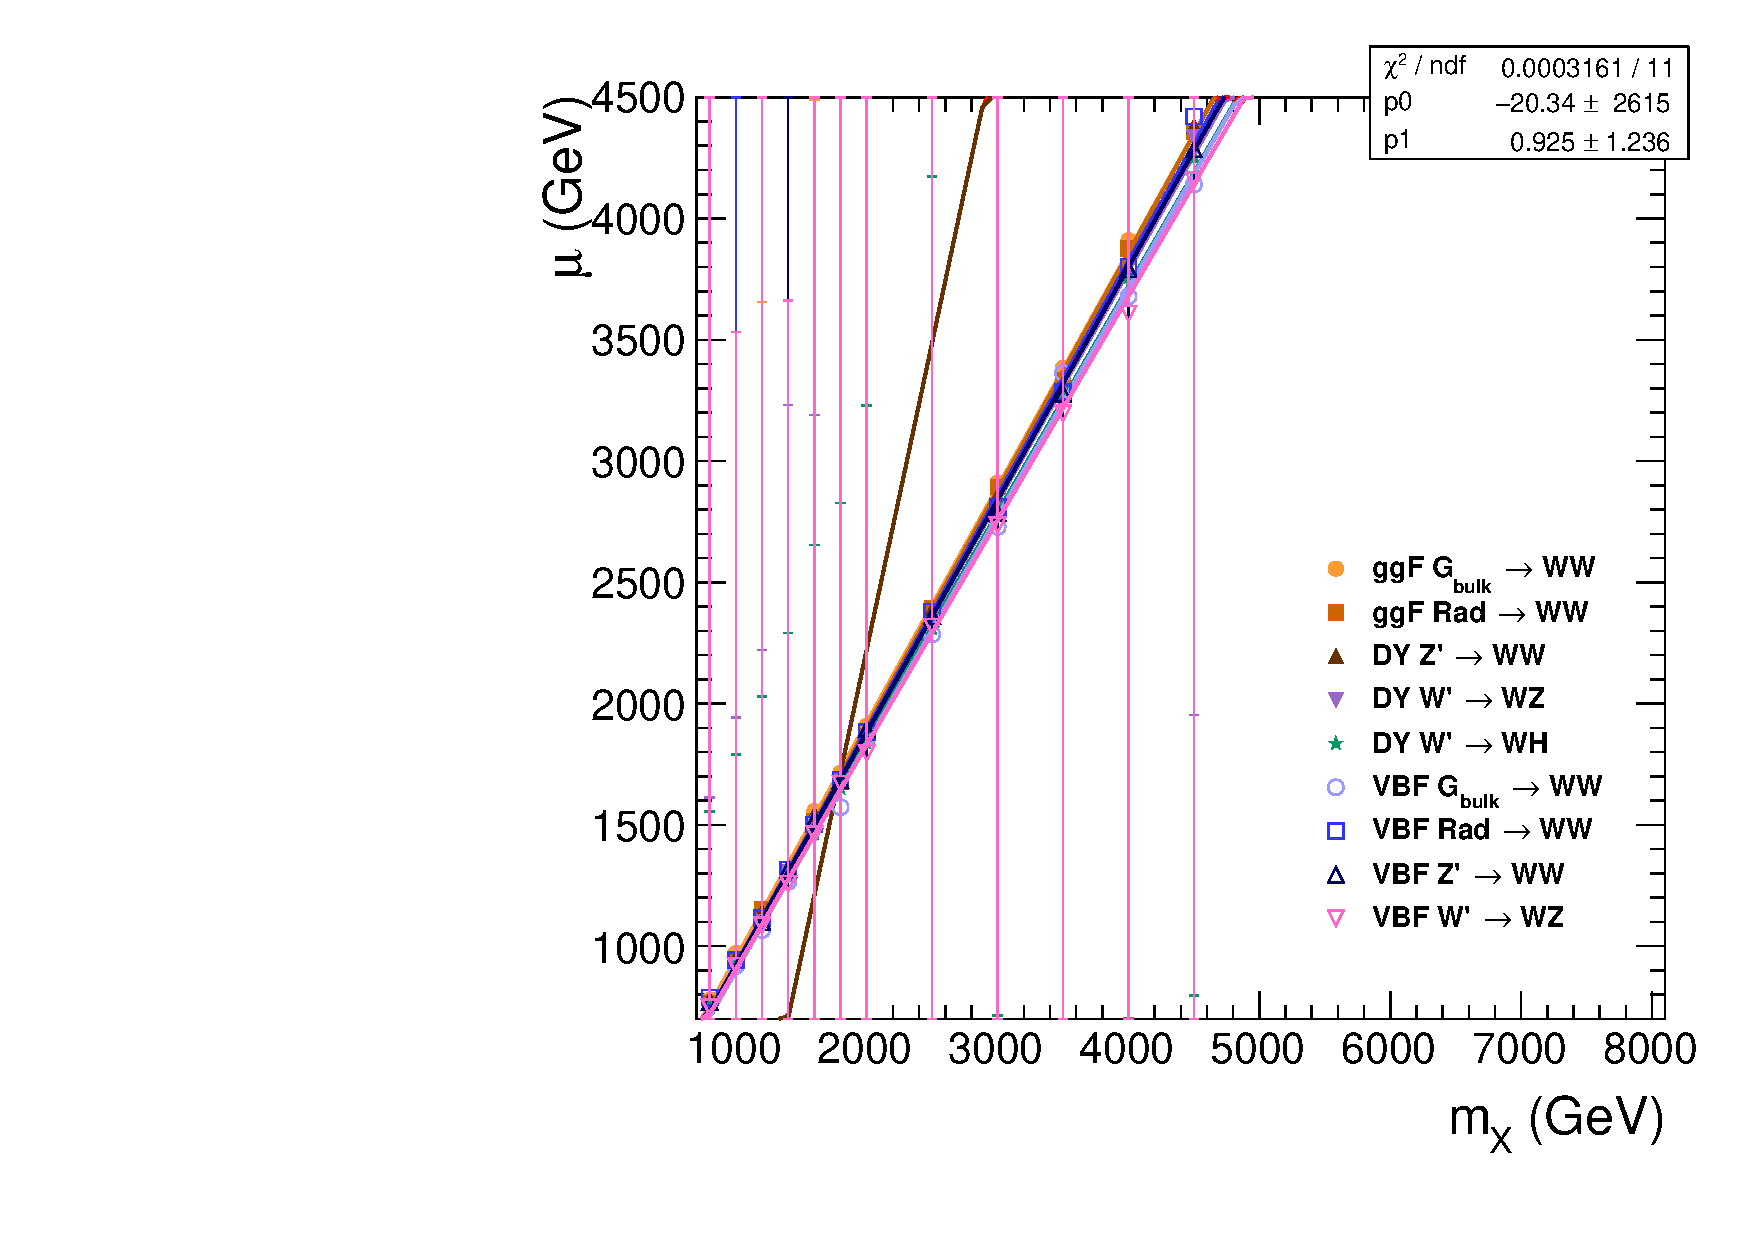
\includegraphics[width=0.2\textwidth]{fig/2Dfit/paramSignalShape_allSig_MVV_LP_bb_HDy_MEAN.pdf}
  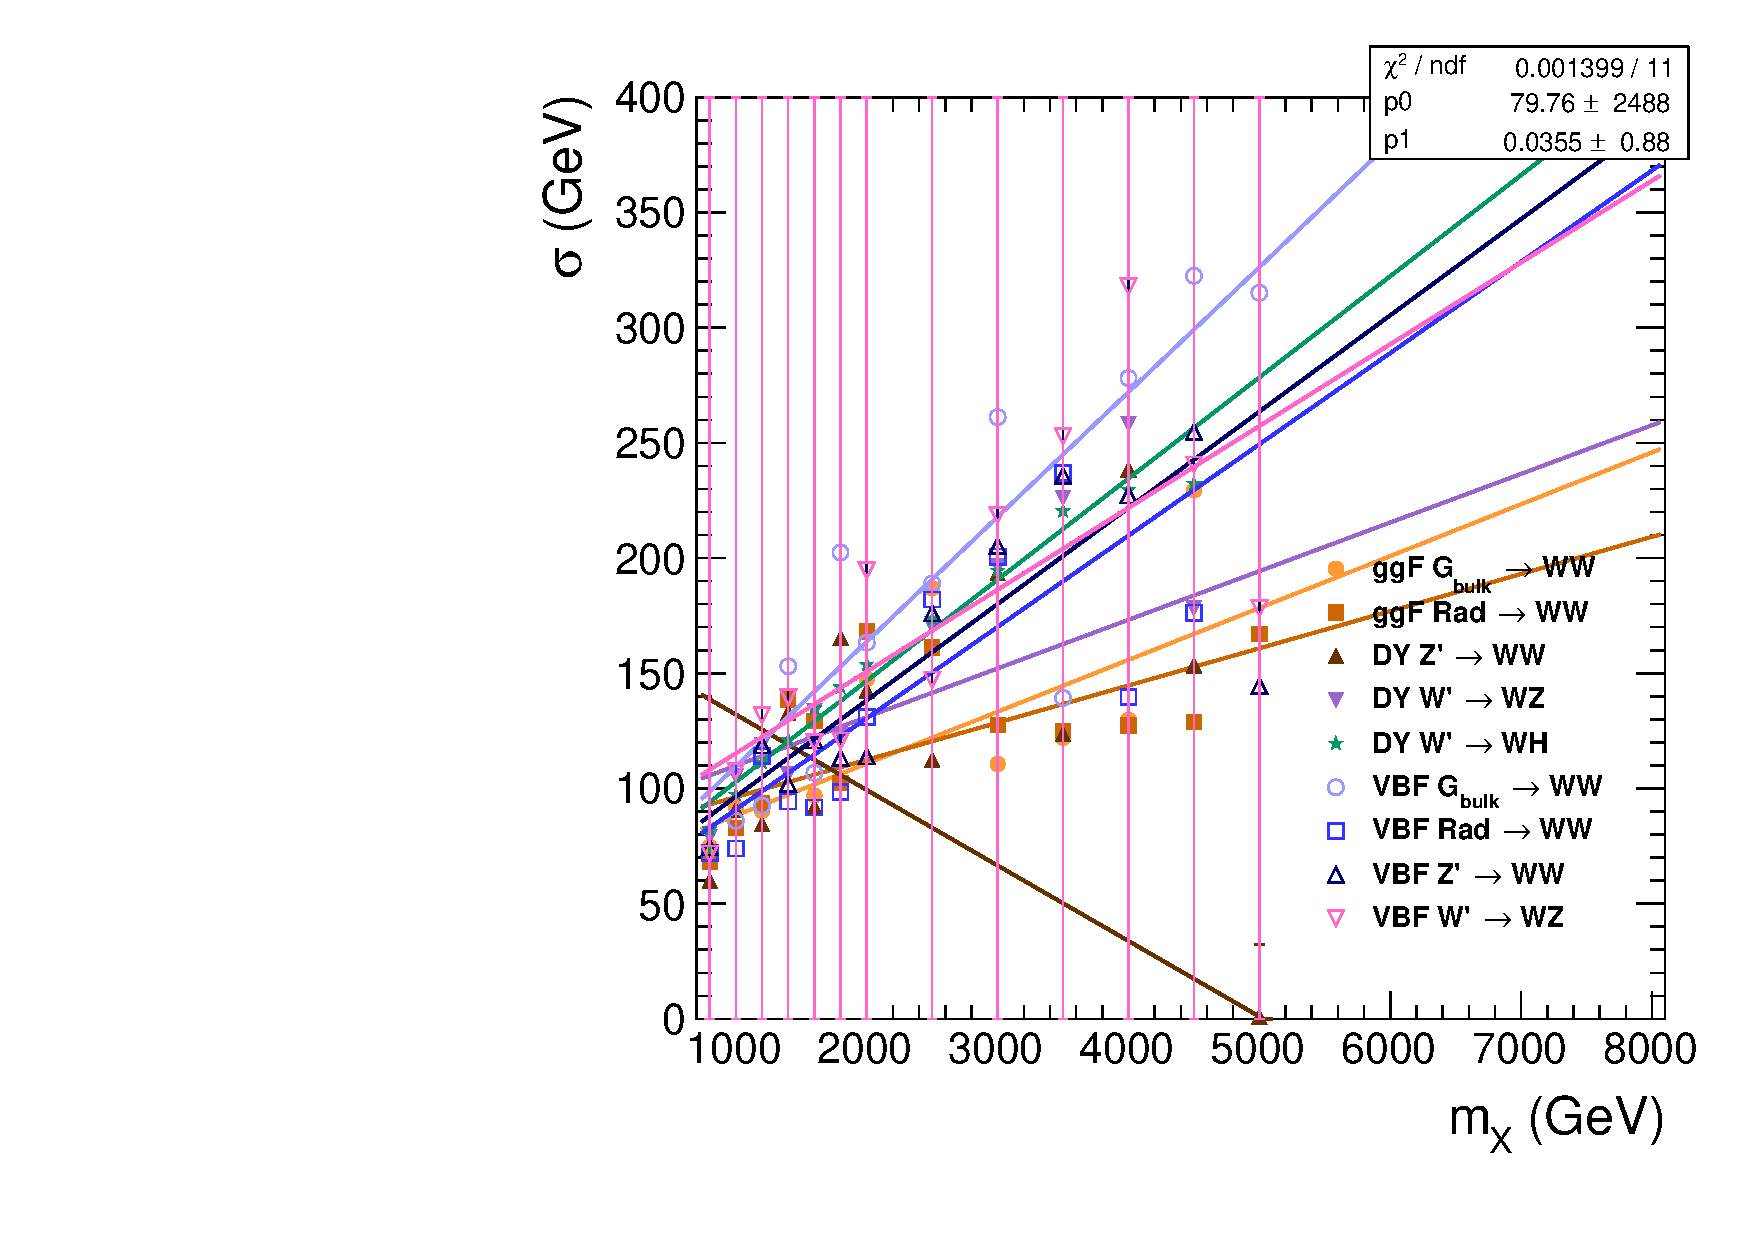
\includegraphics[width=0.2\textwidth]{fig/2Dfit/paramSignalShape_allSig_MVV_LP_bb_HDy_SIGMA.pdf}
  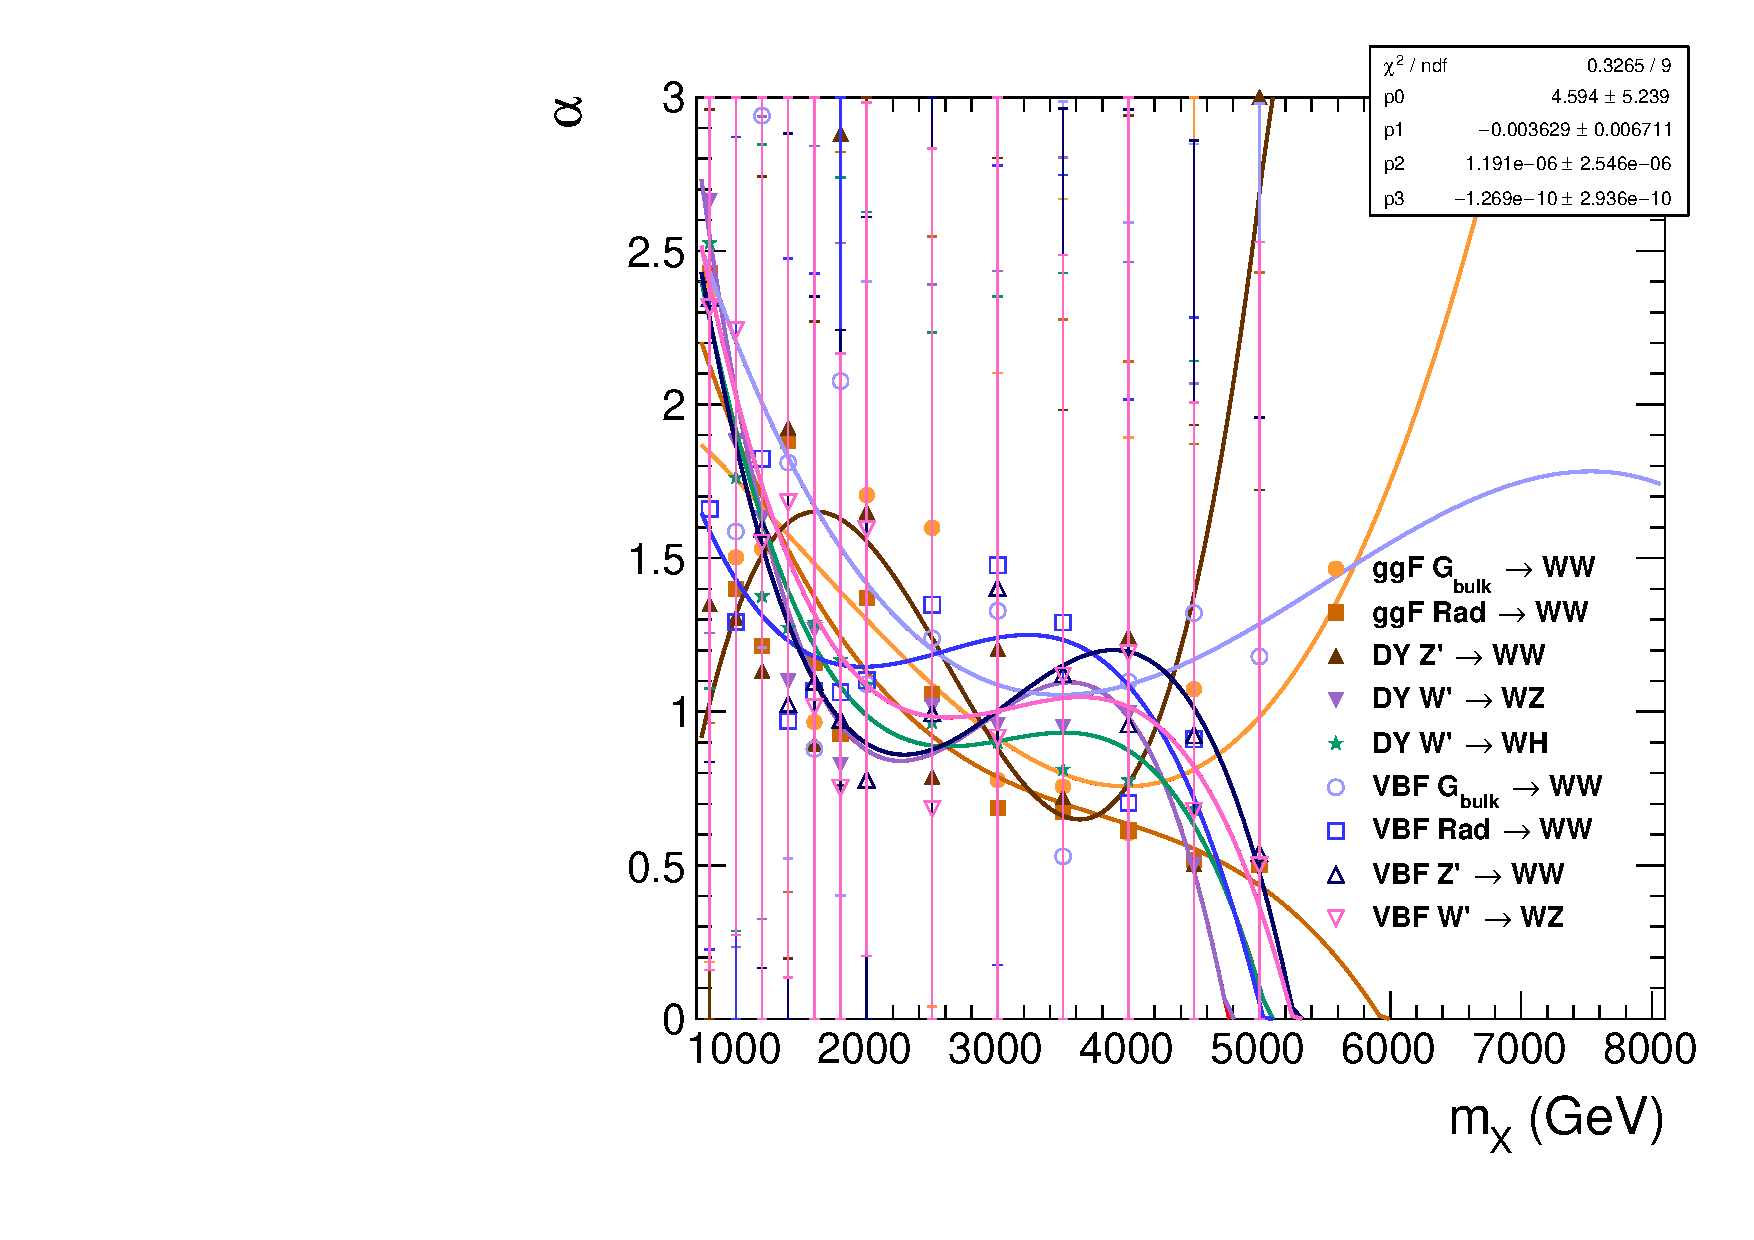
\includegraphics[width=0.2\textwidth]{fig/2Dfit/paramSignalShape_allSig_MVV_LP_bb_HDy_ALPHA1.pdf}
  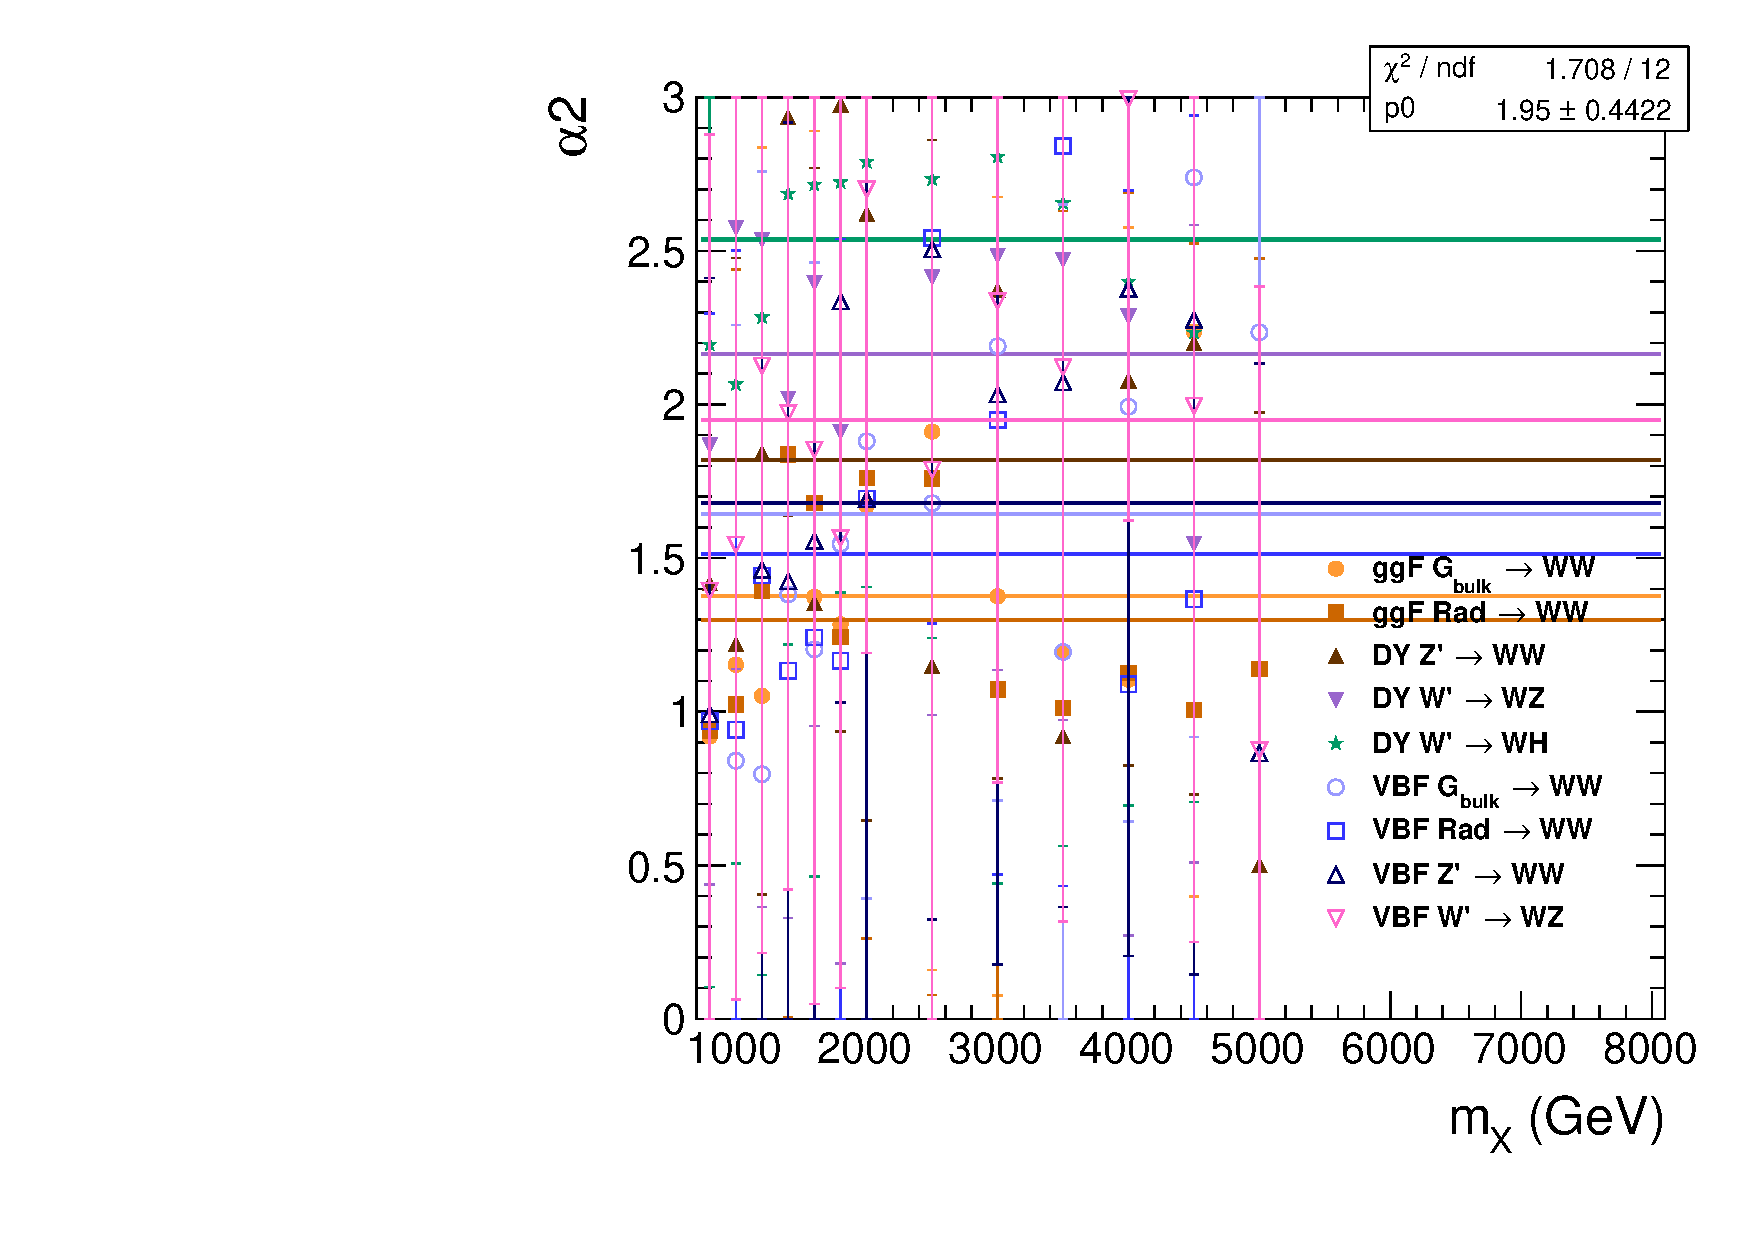
\includegraphics[width=0.2\textwidth]{fig/2Dfit/paramSignalShape_allSig_MVV_LP_bb_HDy_ALPHA2.pdf}\\
  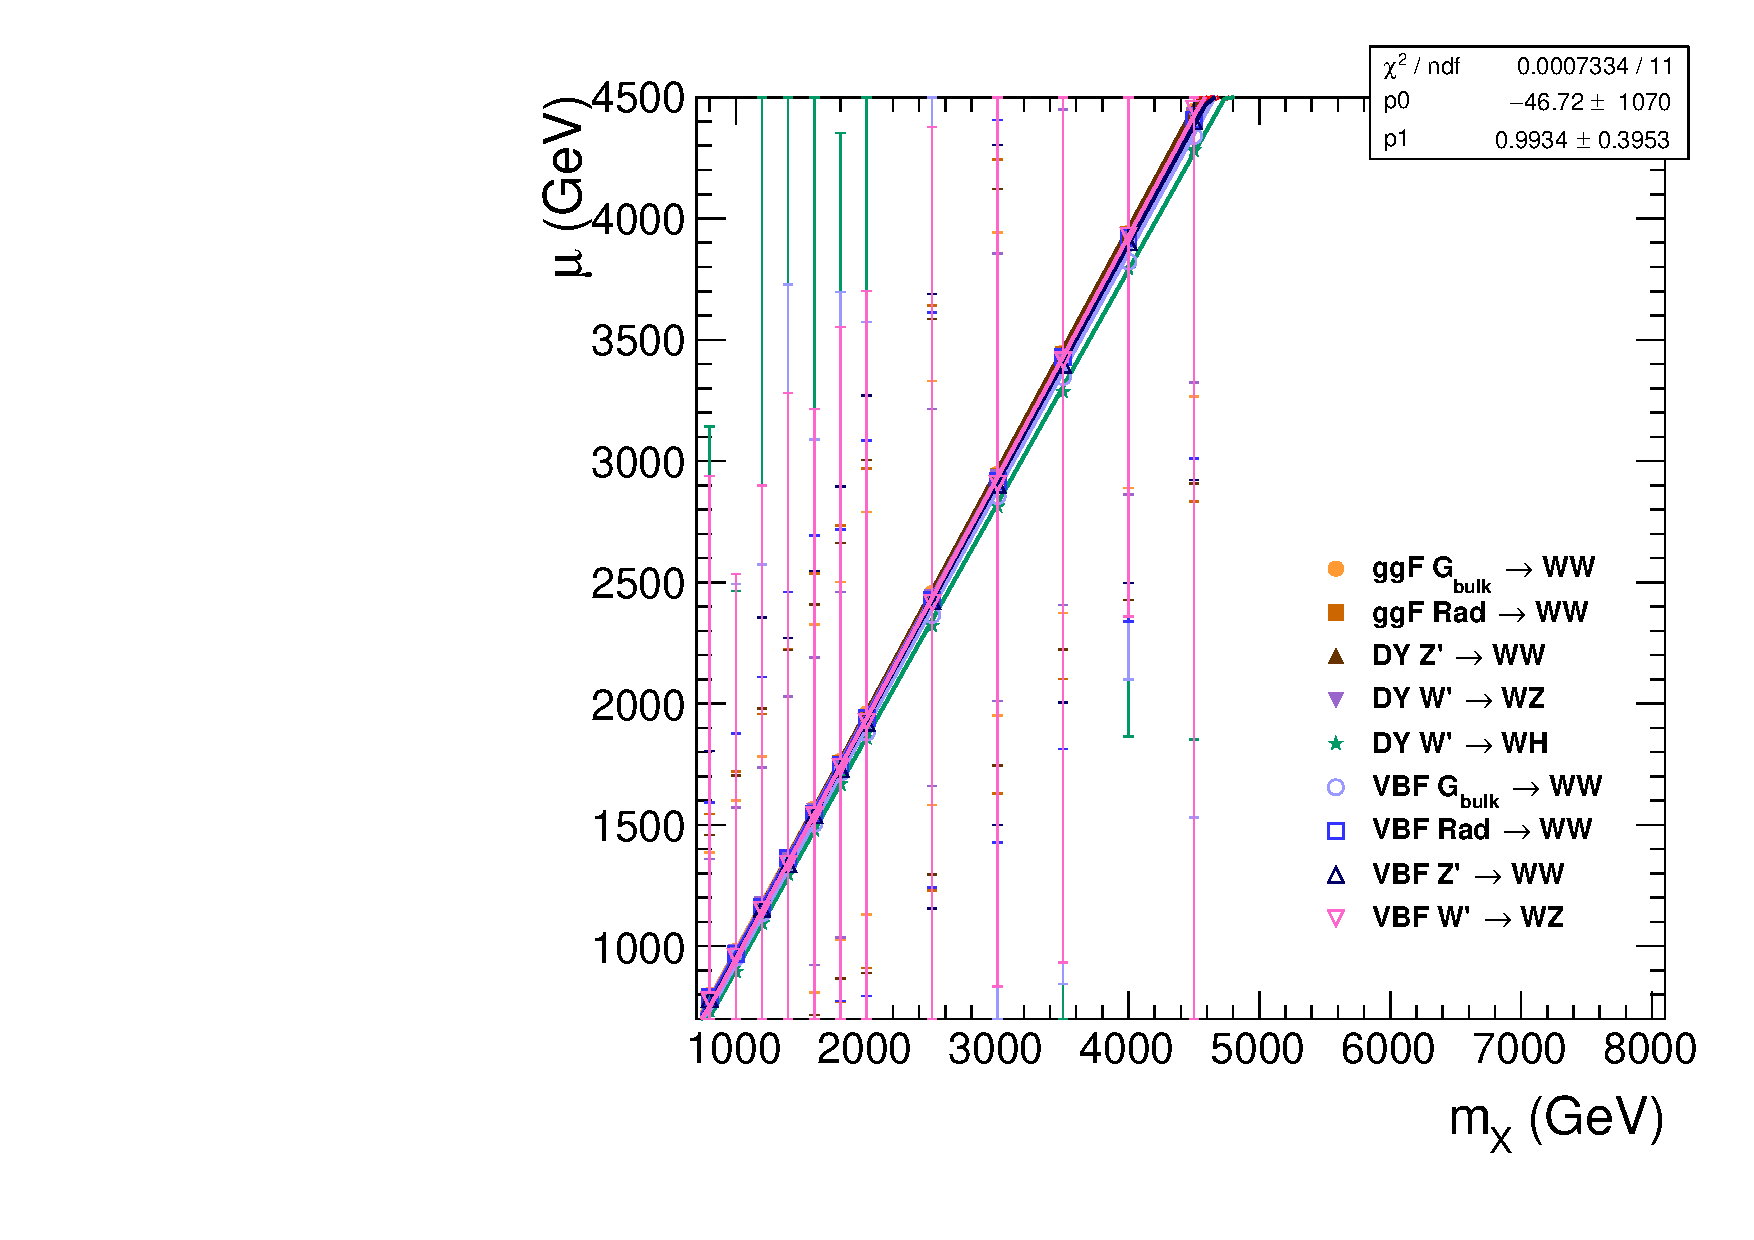
\includegraphics[width=0.2\textwidth]{fig/2Dfit/paramSignalShape_allSig_MVV_HP_nobb_HDy_MEAN.pdf}
  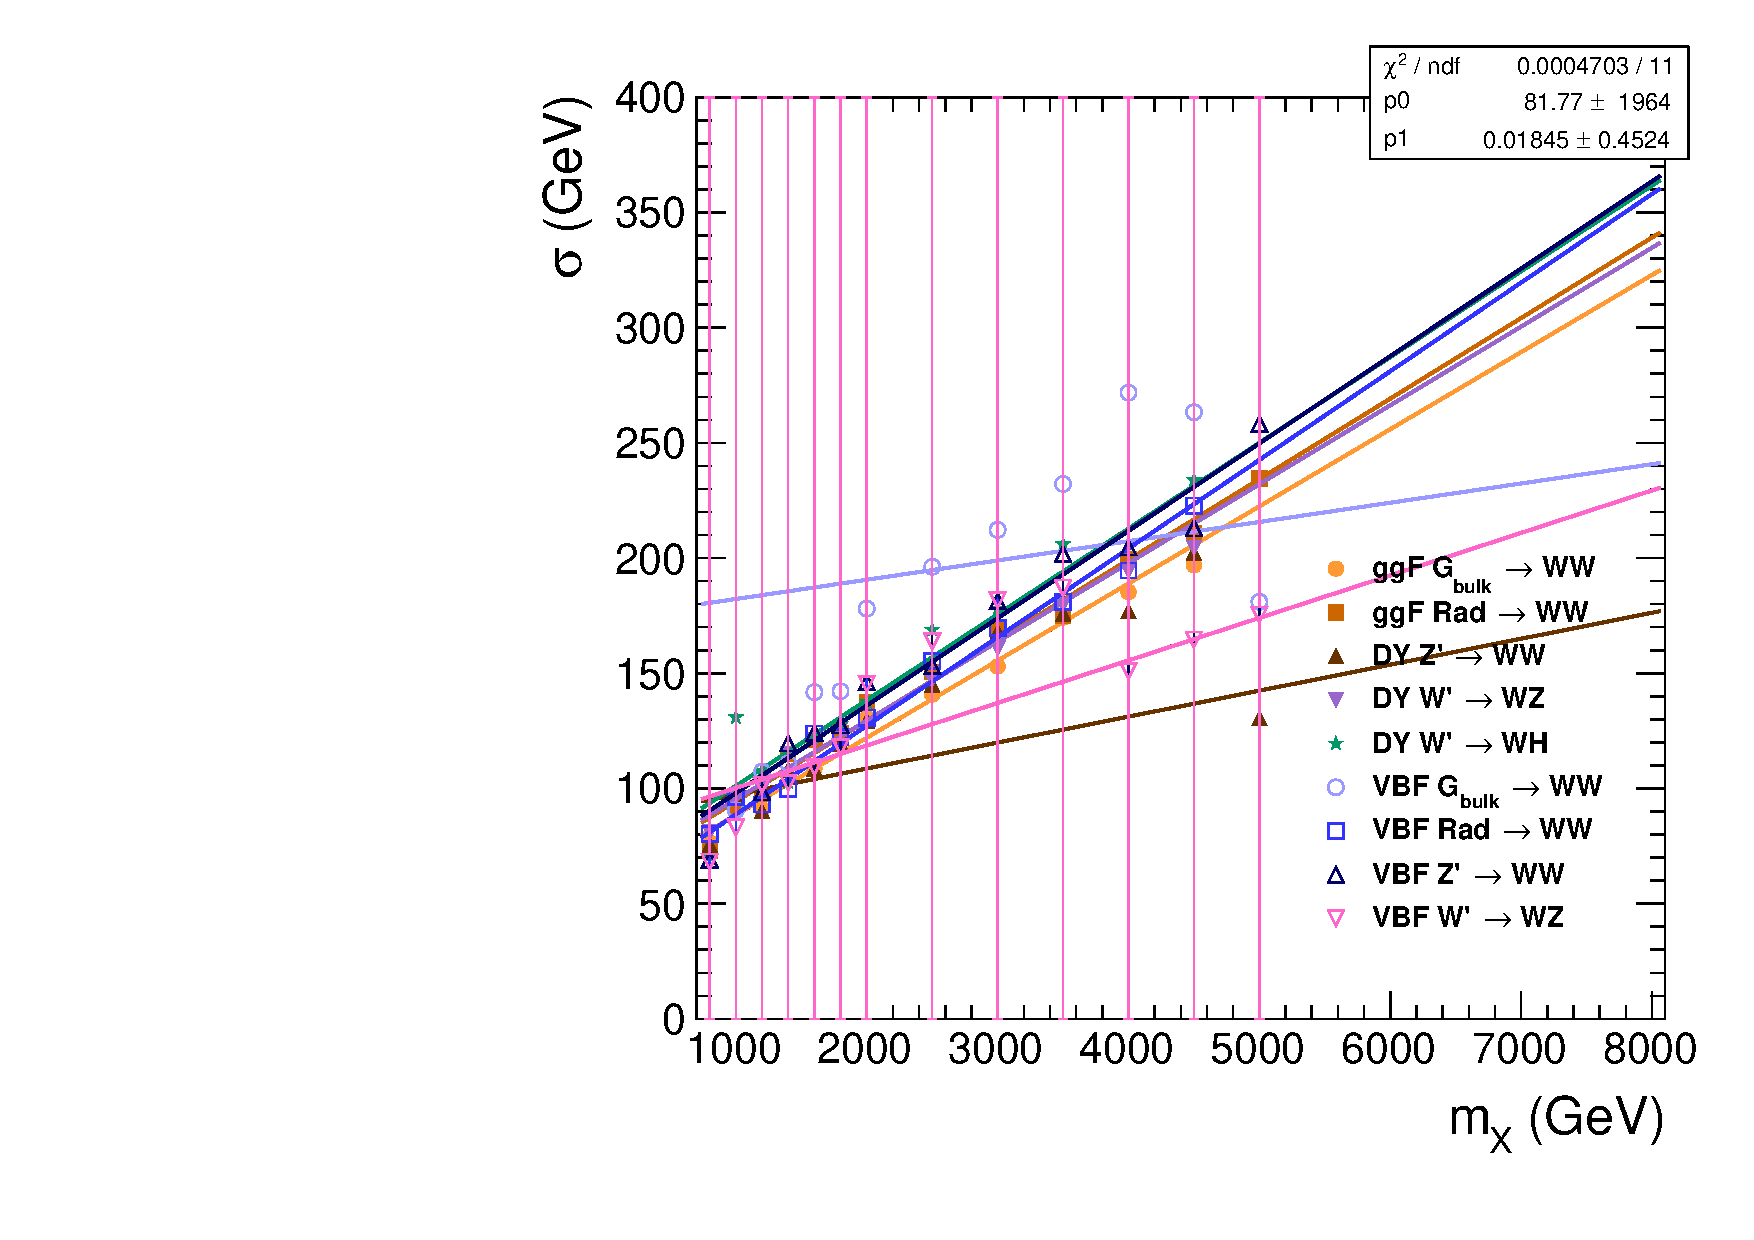
\includegraphics[width=0.2\textwidth]{fig/2Dfit/paramSignalShape_allSig_MVV_HP_nobb_HDy_SIGMA.pdf}
  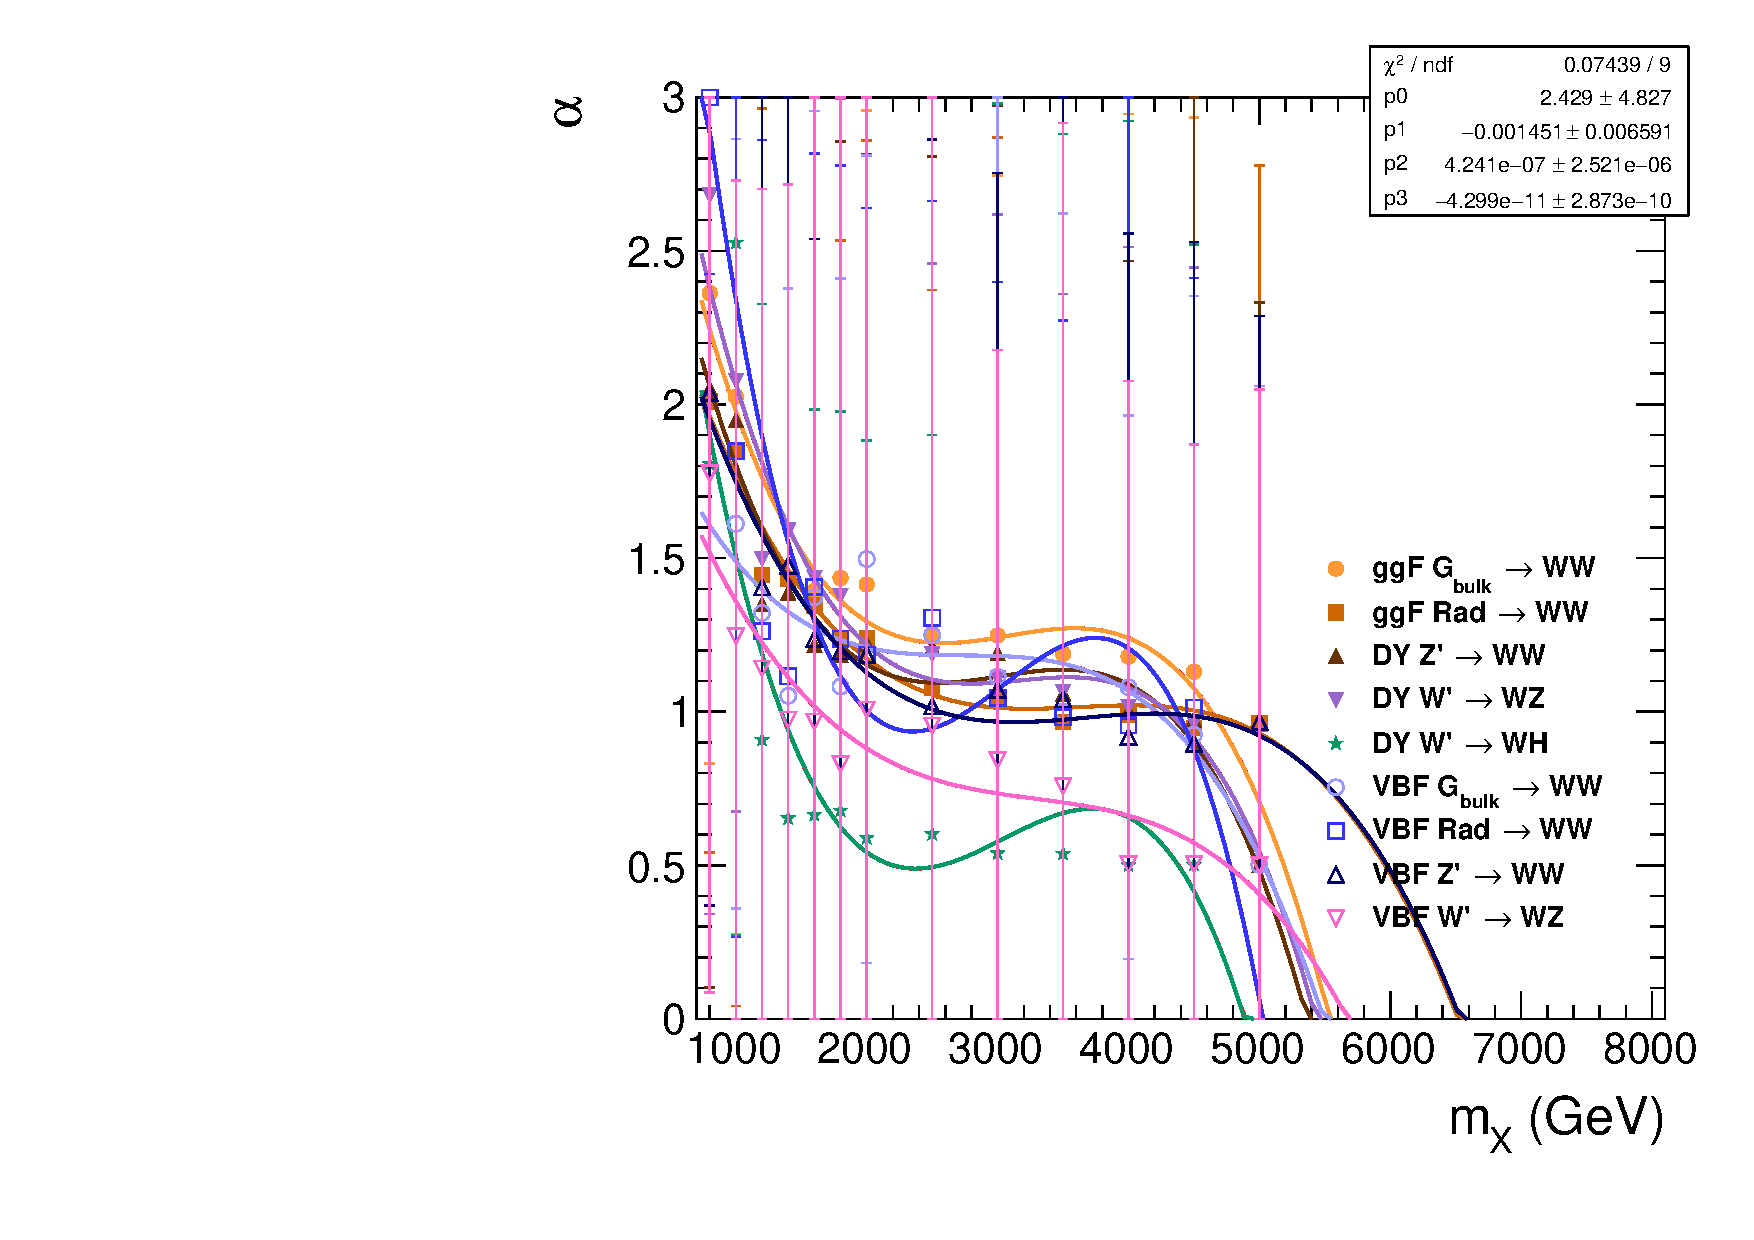
\includegraphics[width=0.2\textwidth]{fig/2Dfit/paramSignalShape_allSig_MVV_HP_nobb_HDy_ALPHA1.pdf}
  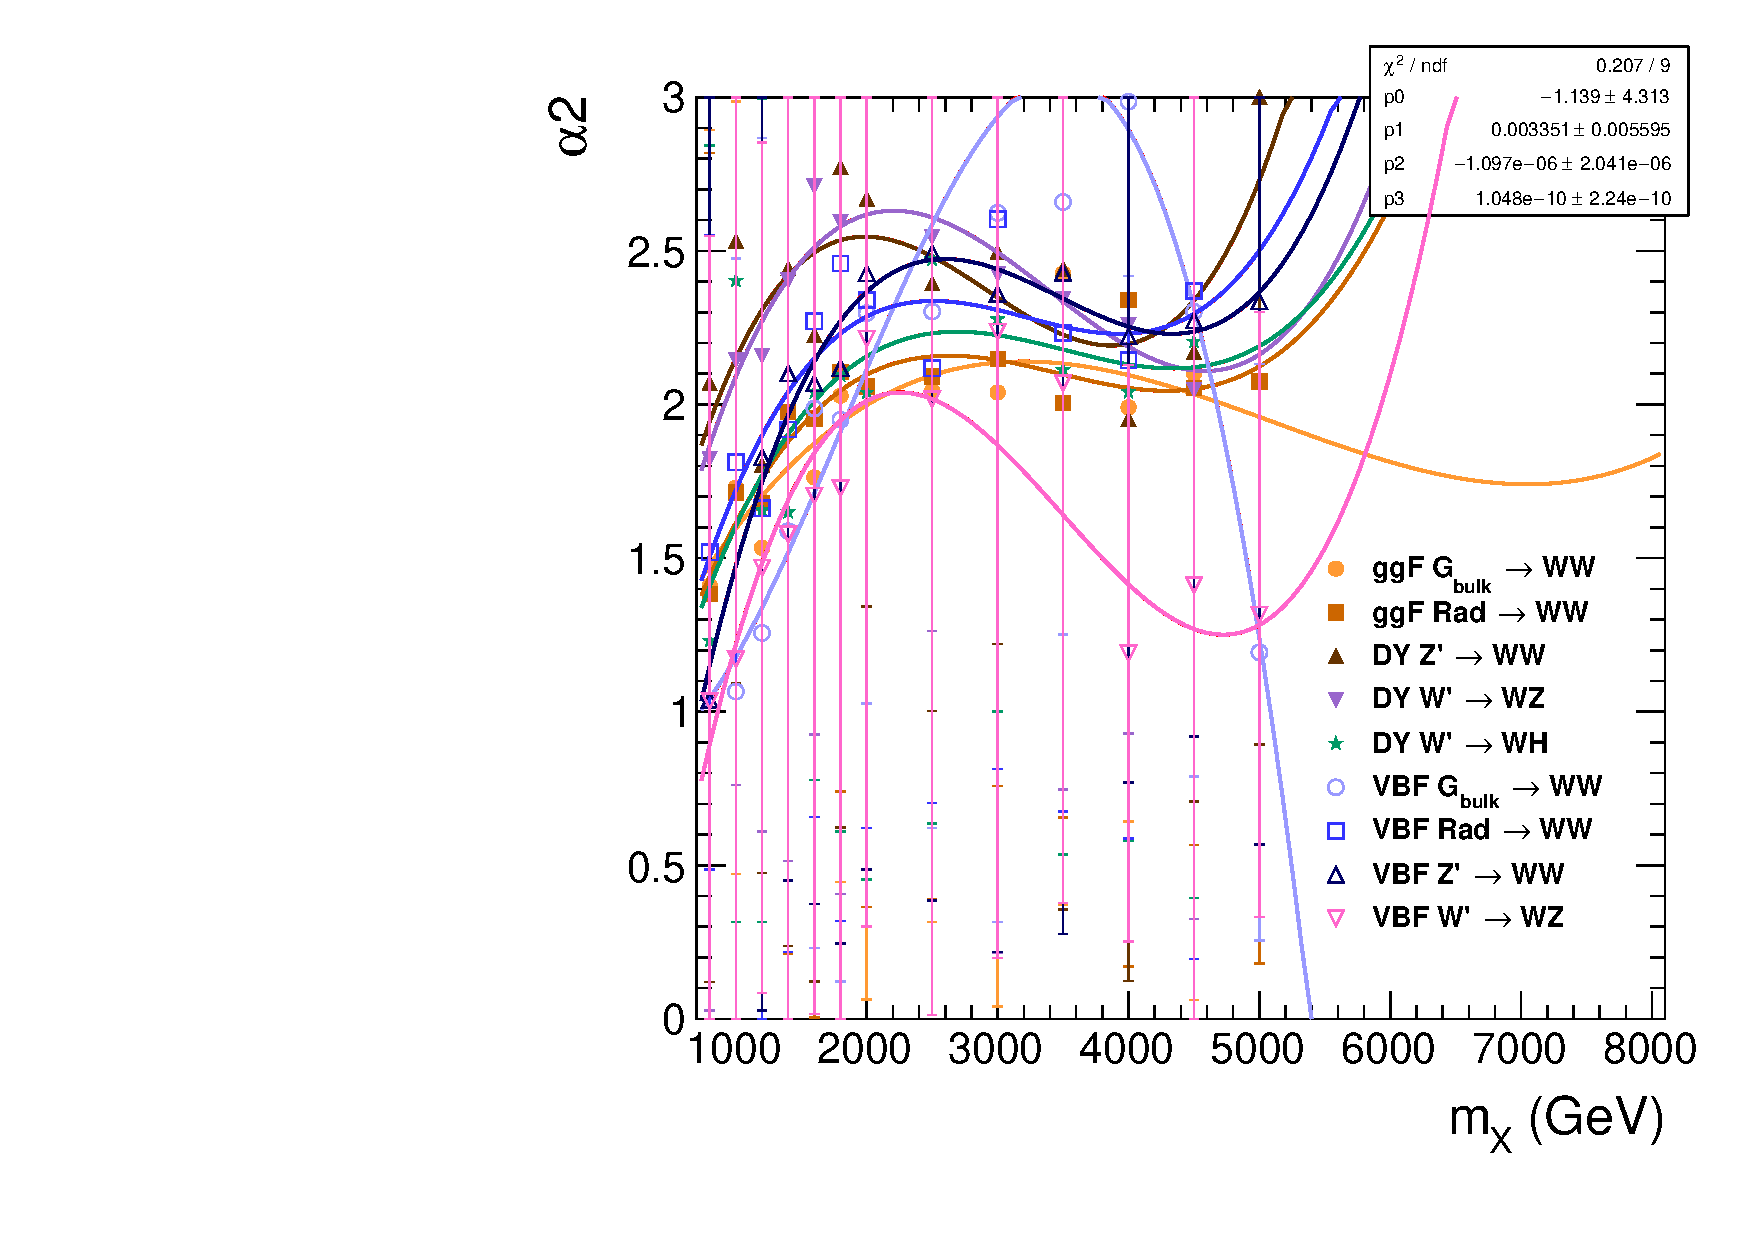
\includegraphics[width=0.2\textwidth]{fig/2Dfit/paramSignalShape_allSig_MVV_HP_nobb_HDy_ALPHA2.pdf}\\
  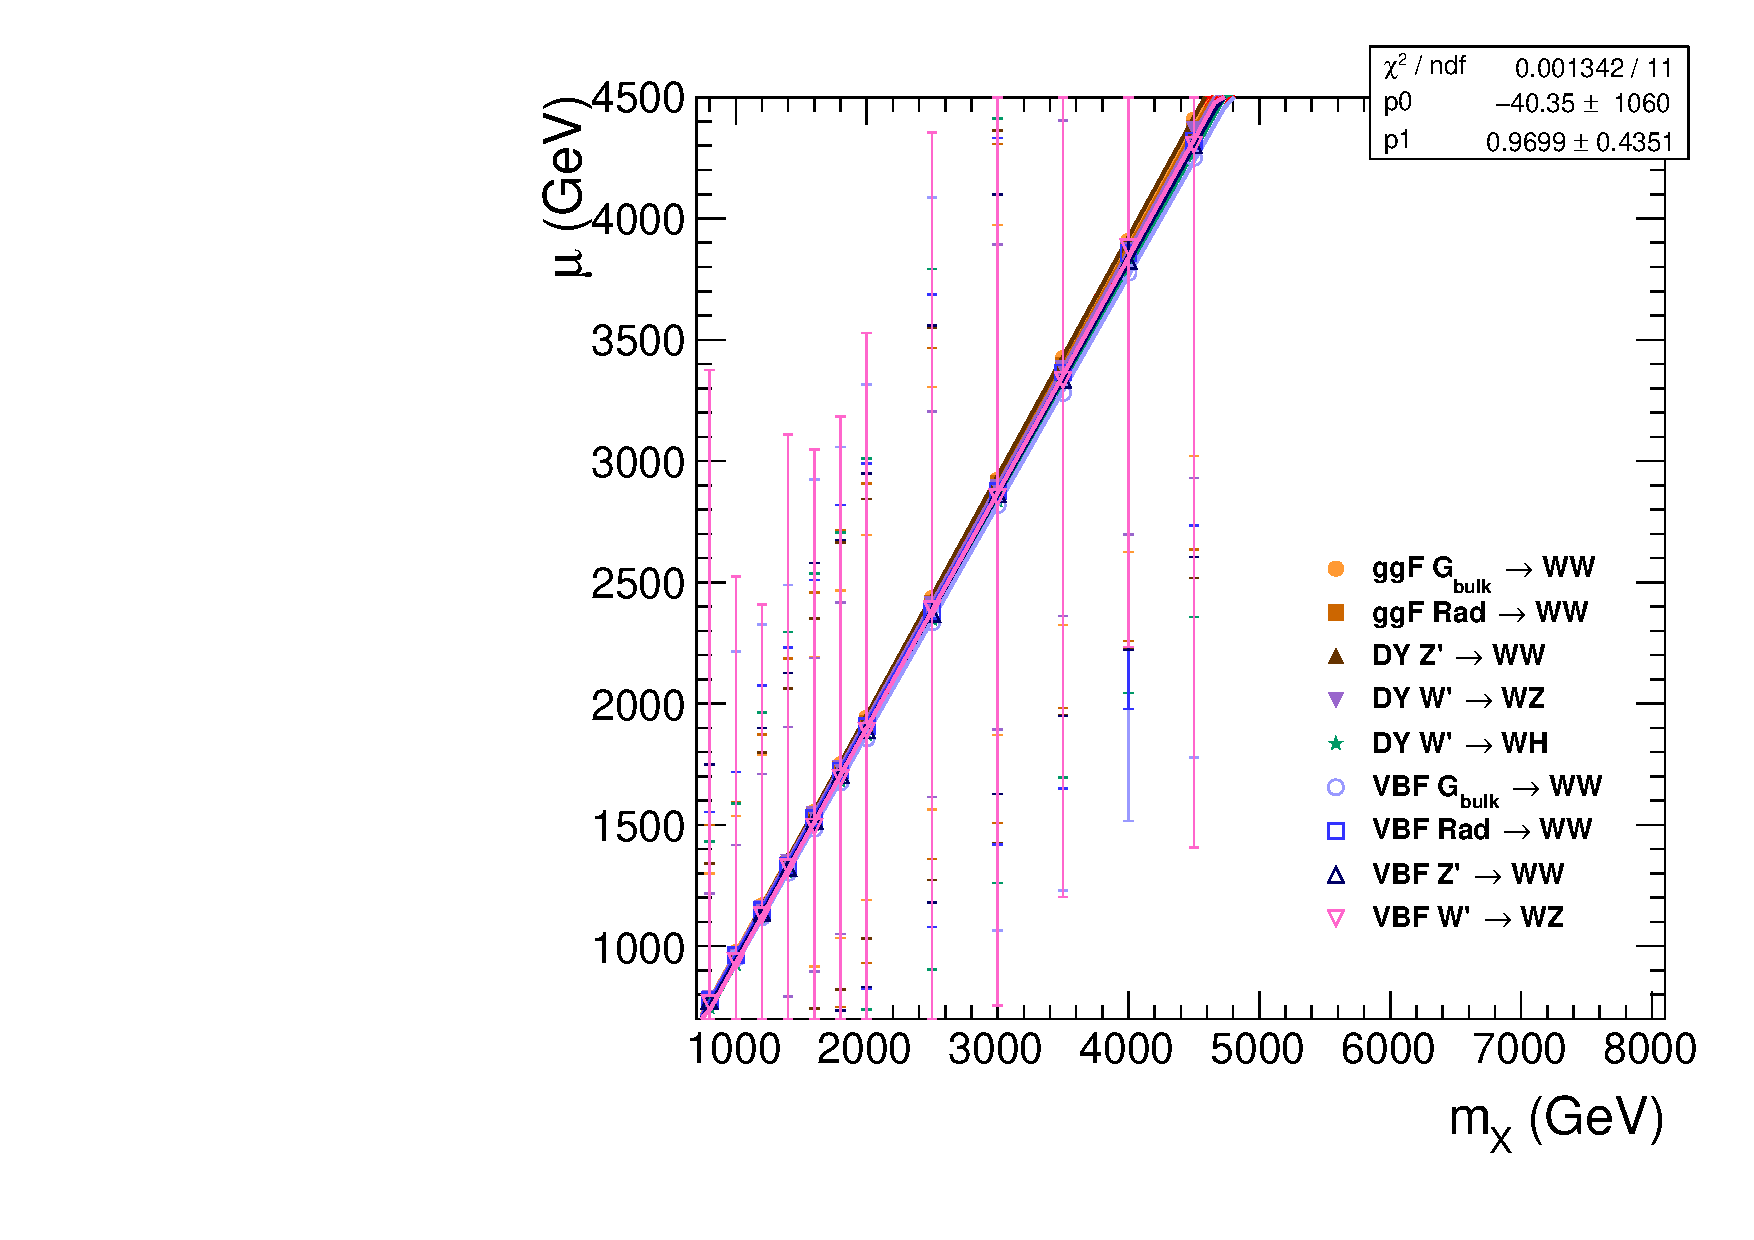
\includegraphics[width=0.2\textwidth]{fig/2Dfit/paramSignalShape_allSig_MVV_LP_nobb_HDy_MEAN.pdf}
  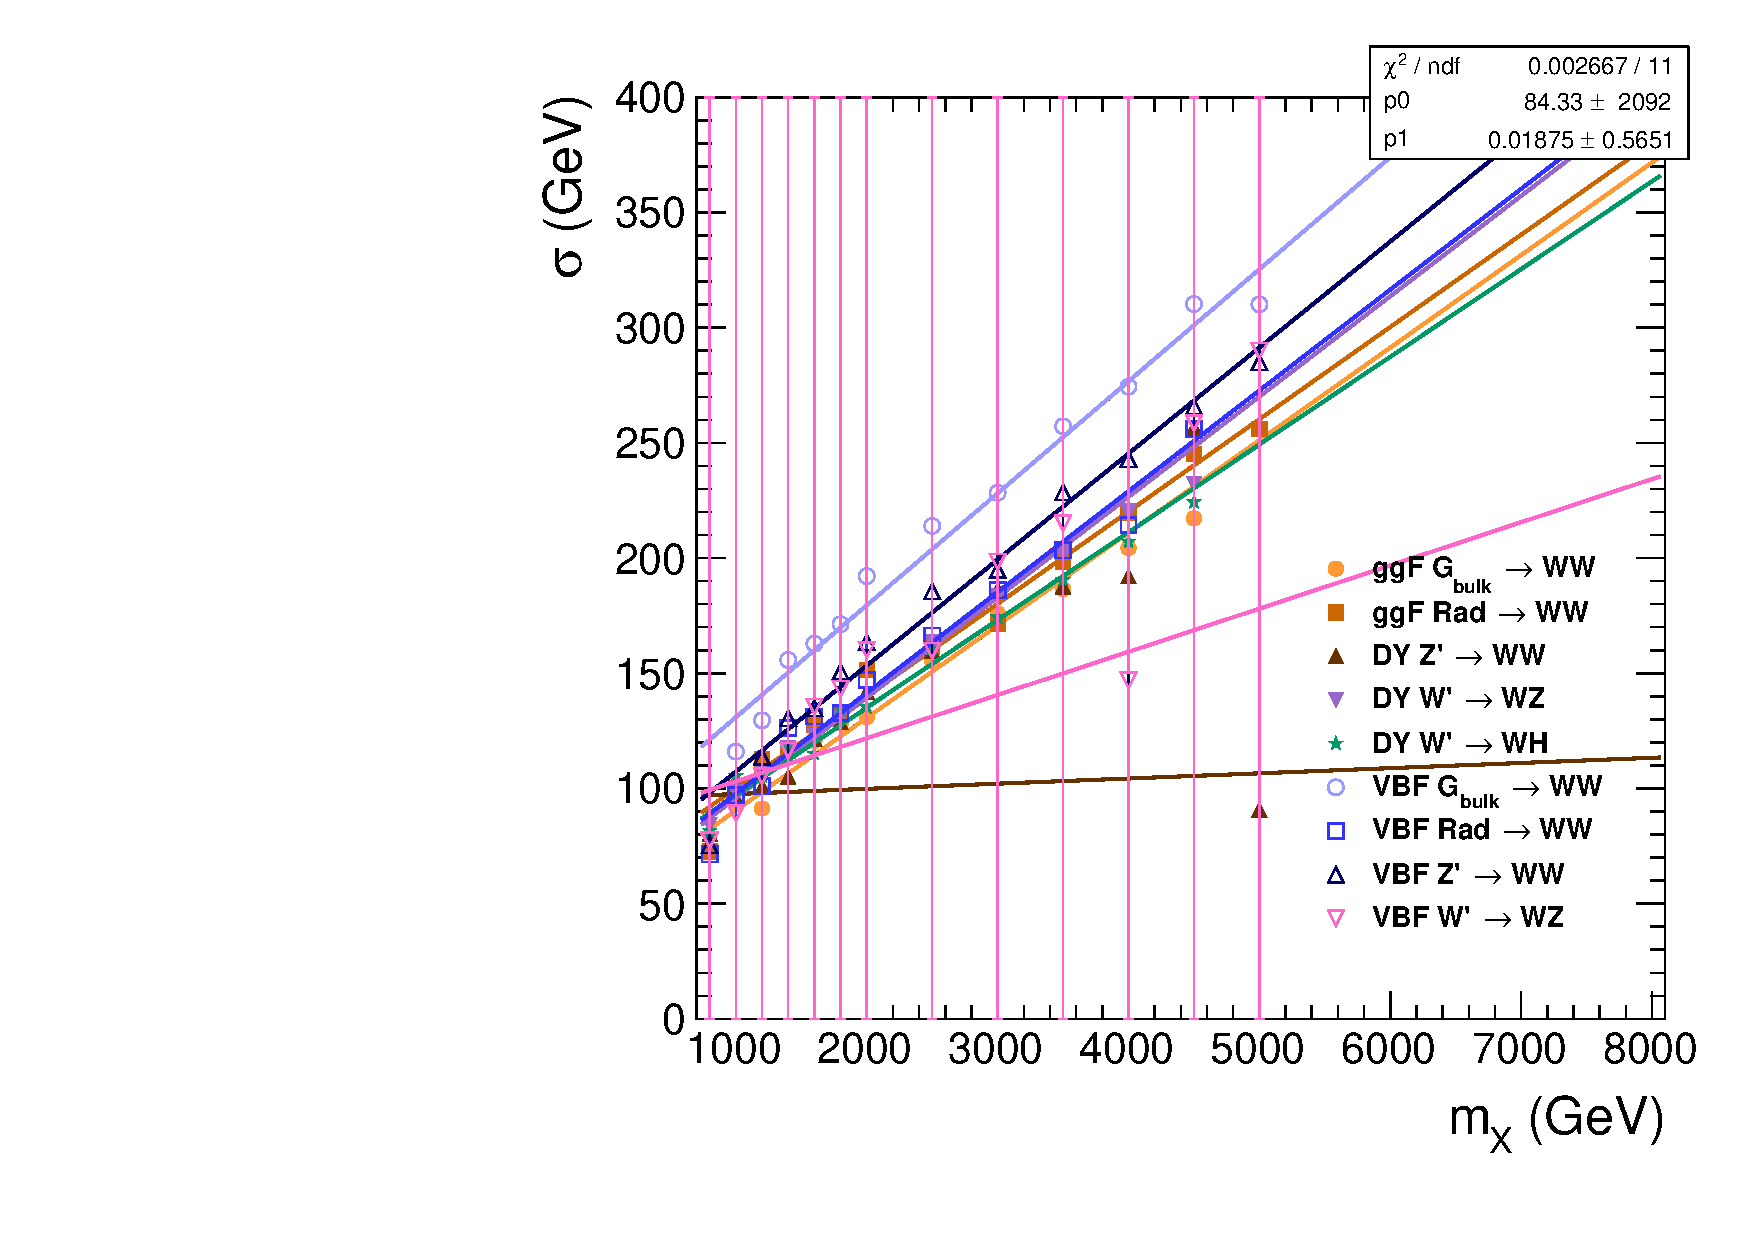
\includegraphics[width=0.2\textwidth]{fig/2Dfit/paramSignalShape_allSig_MVV_LP_nobb_HDy_SIGMA.pdf}
  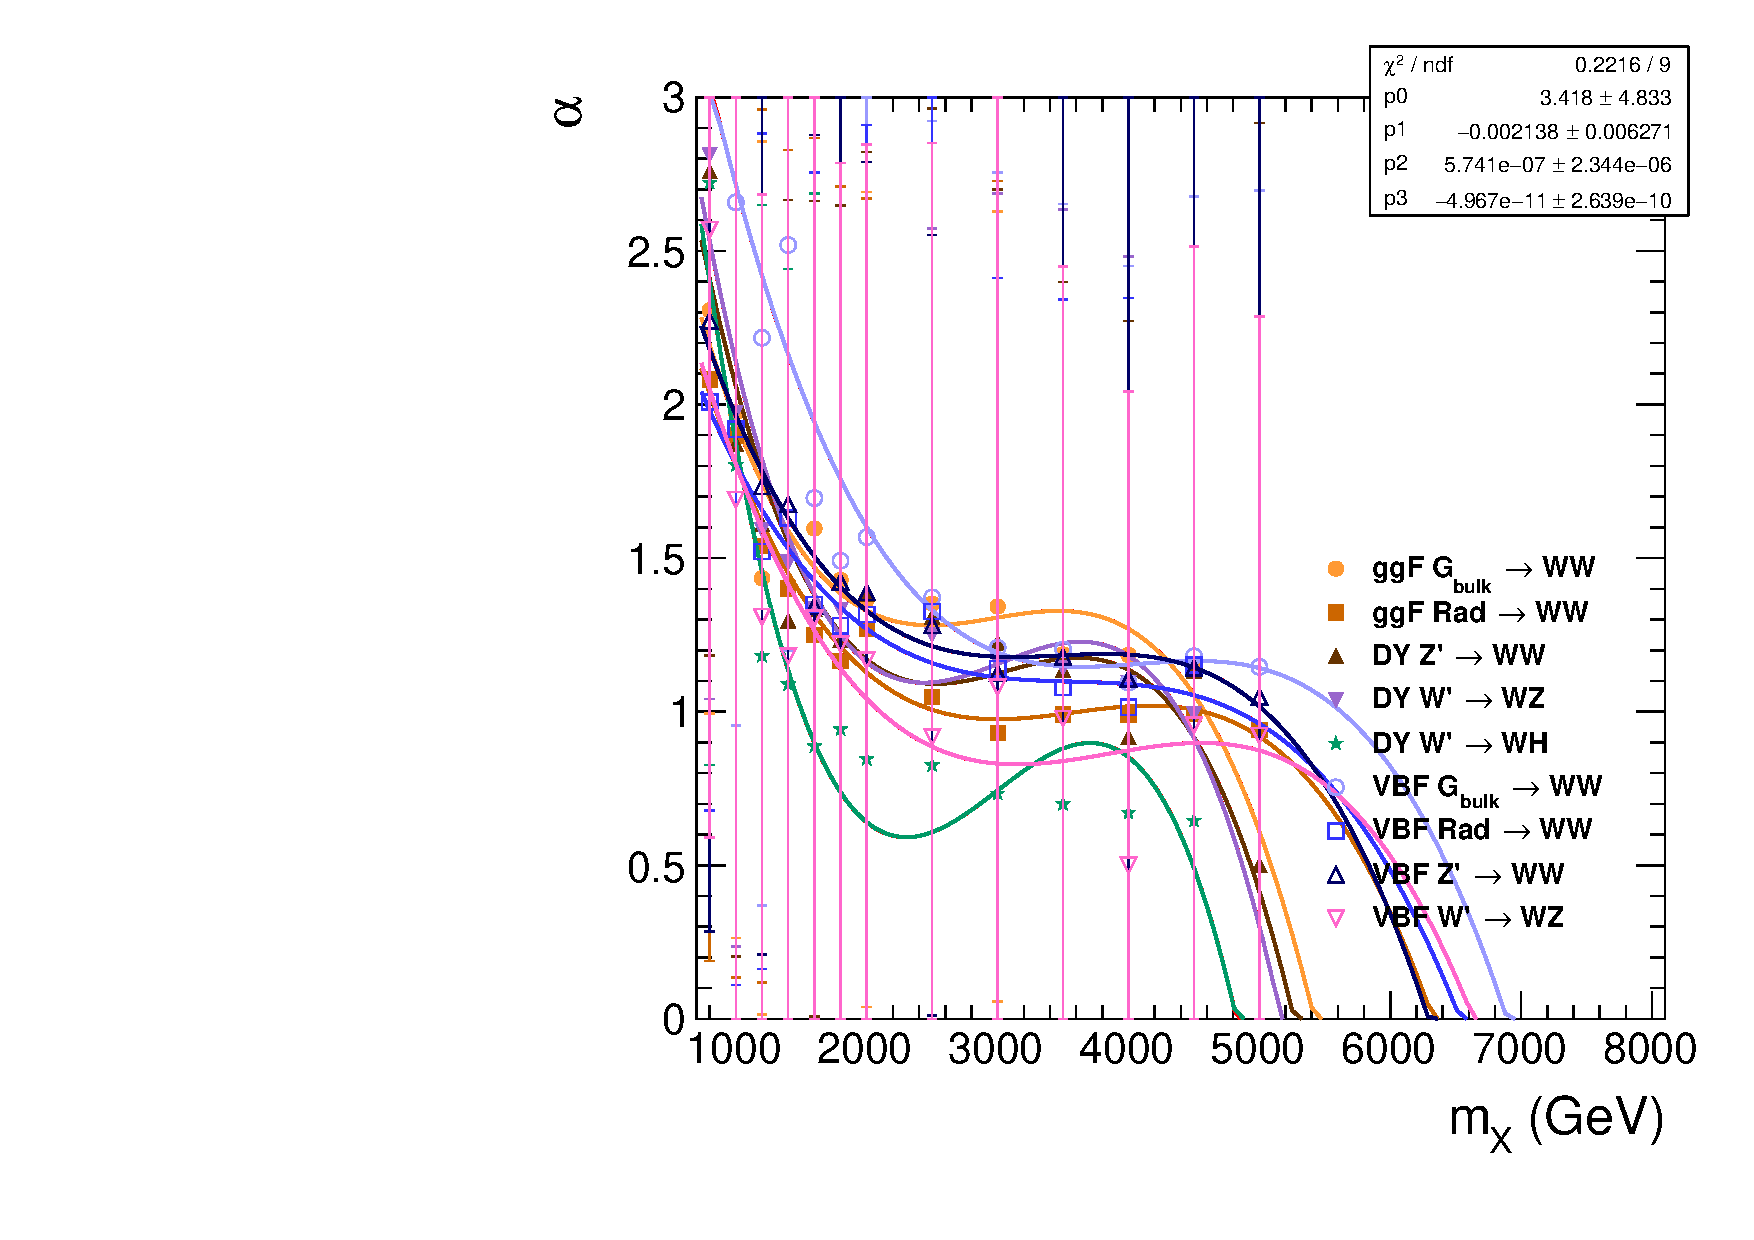
\includegraphics[width=0.2\textwidth]{fig/2Dfit/paramSignalShape_allSig_MVV_LP_nobb_HDy_ALPHA1.pdf}
  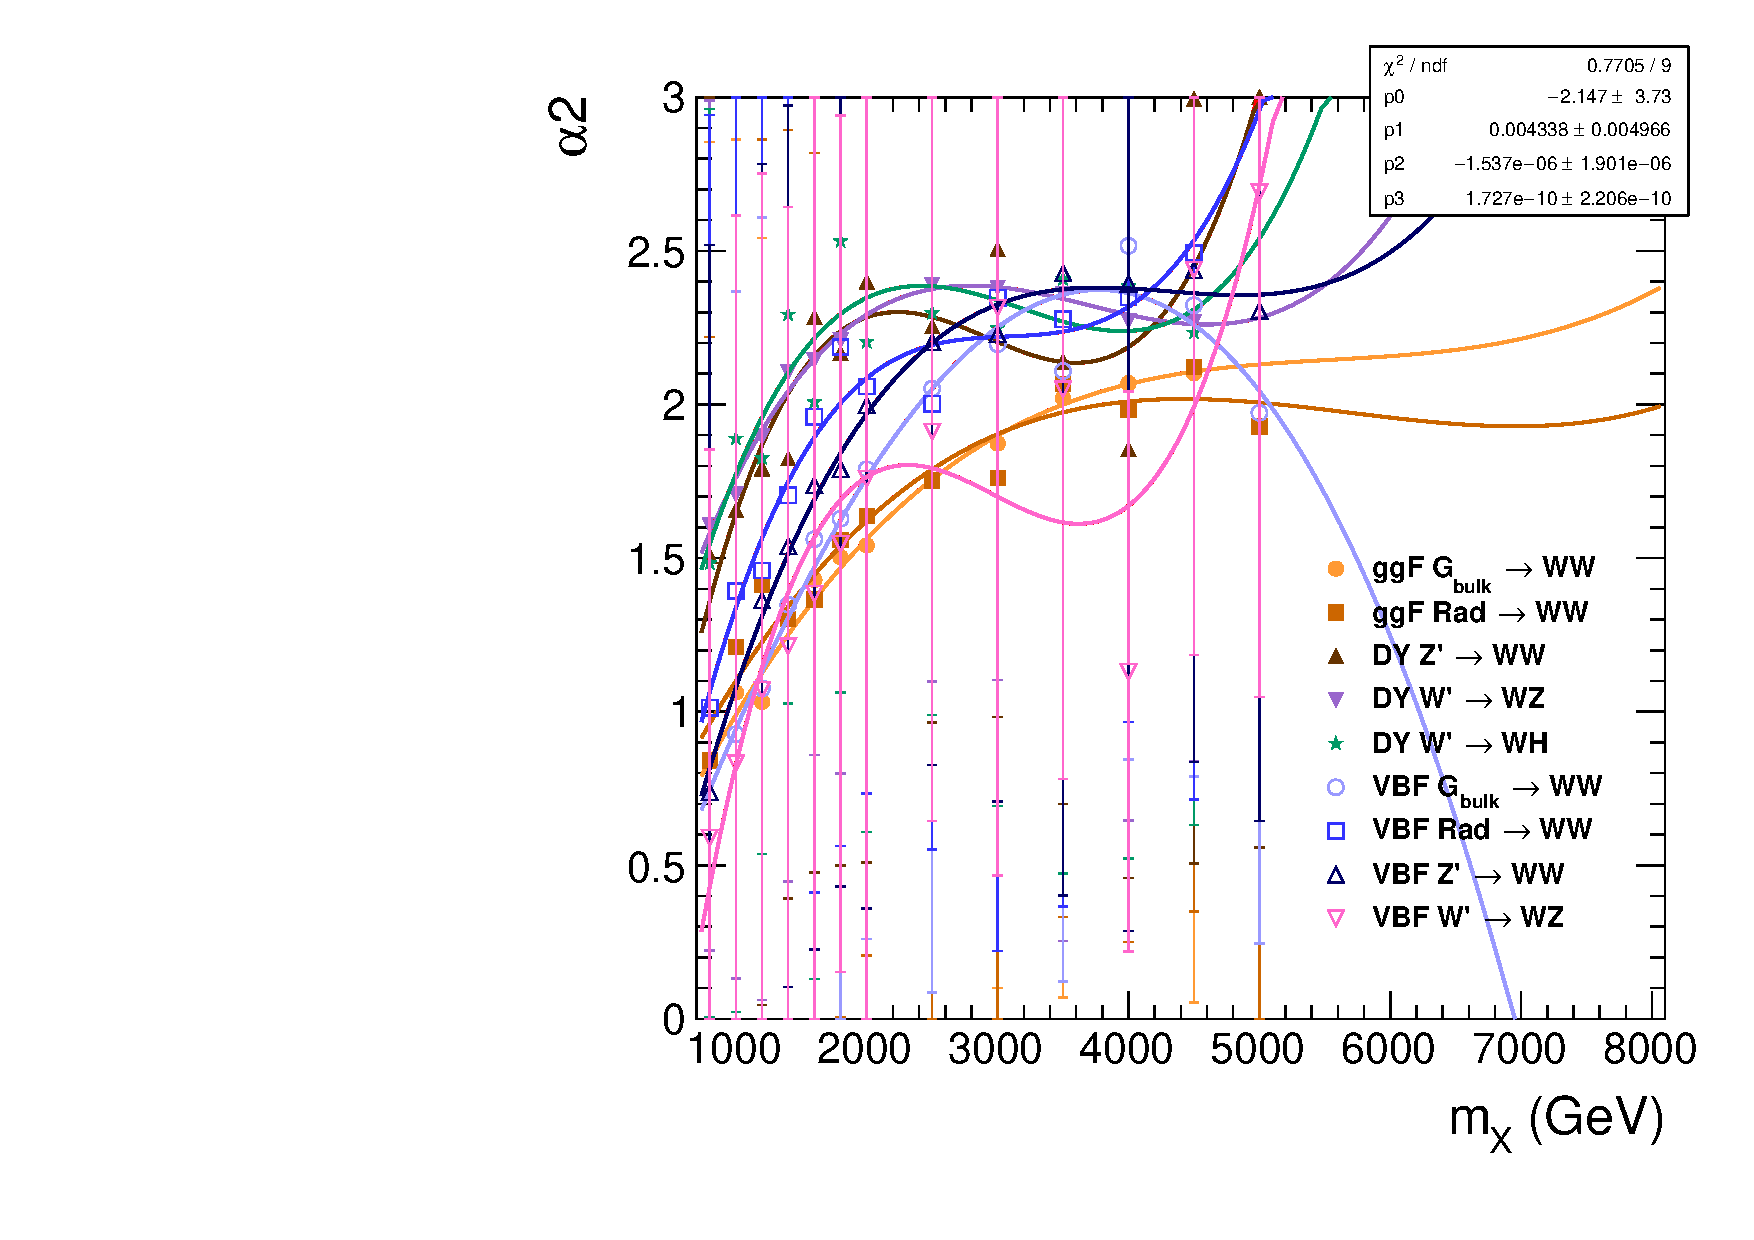
\includegraphics[width=0.2\textwidth]{fig/2Dfit/paramSignalShape_allSig_MVV_LP_nobb_HDy_ALPHA2.pdf}\\
  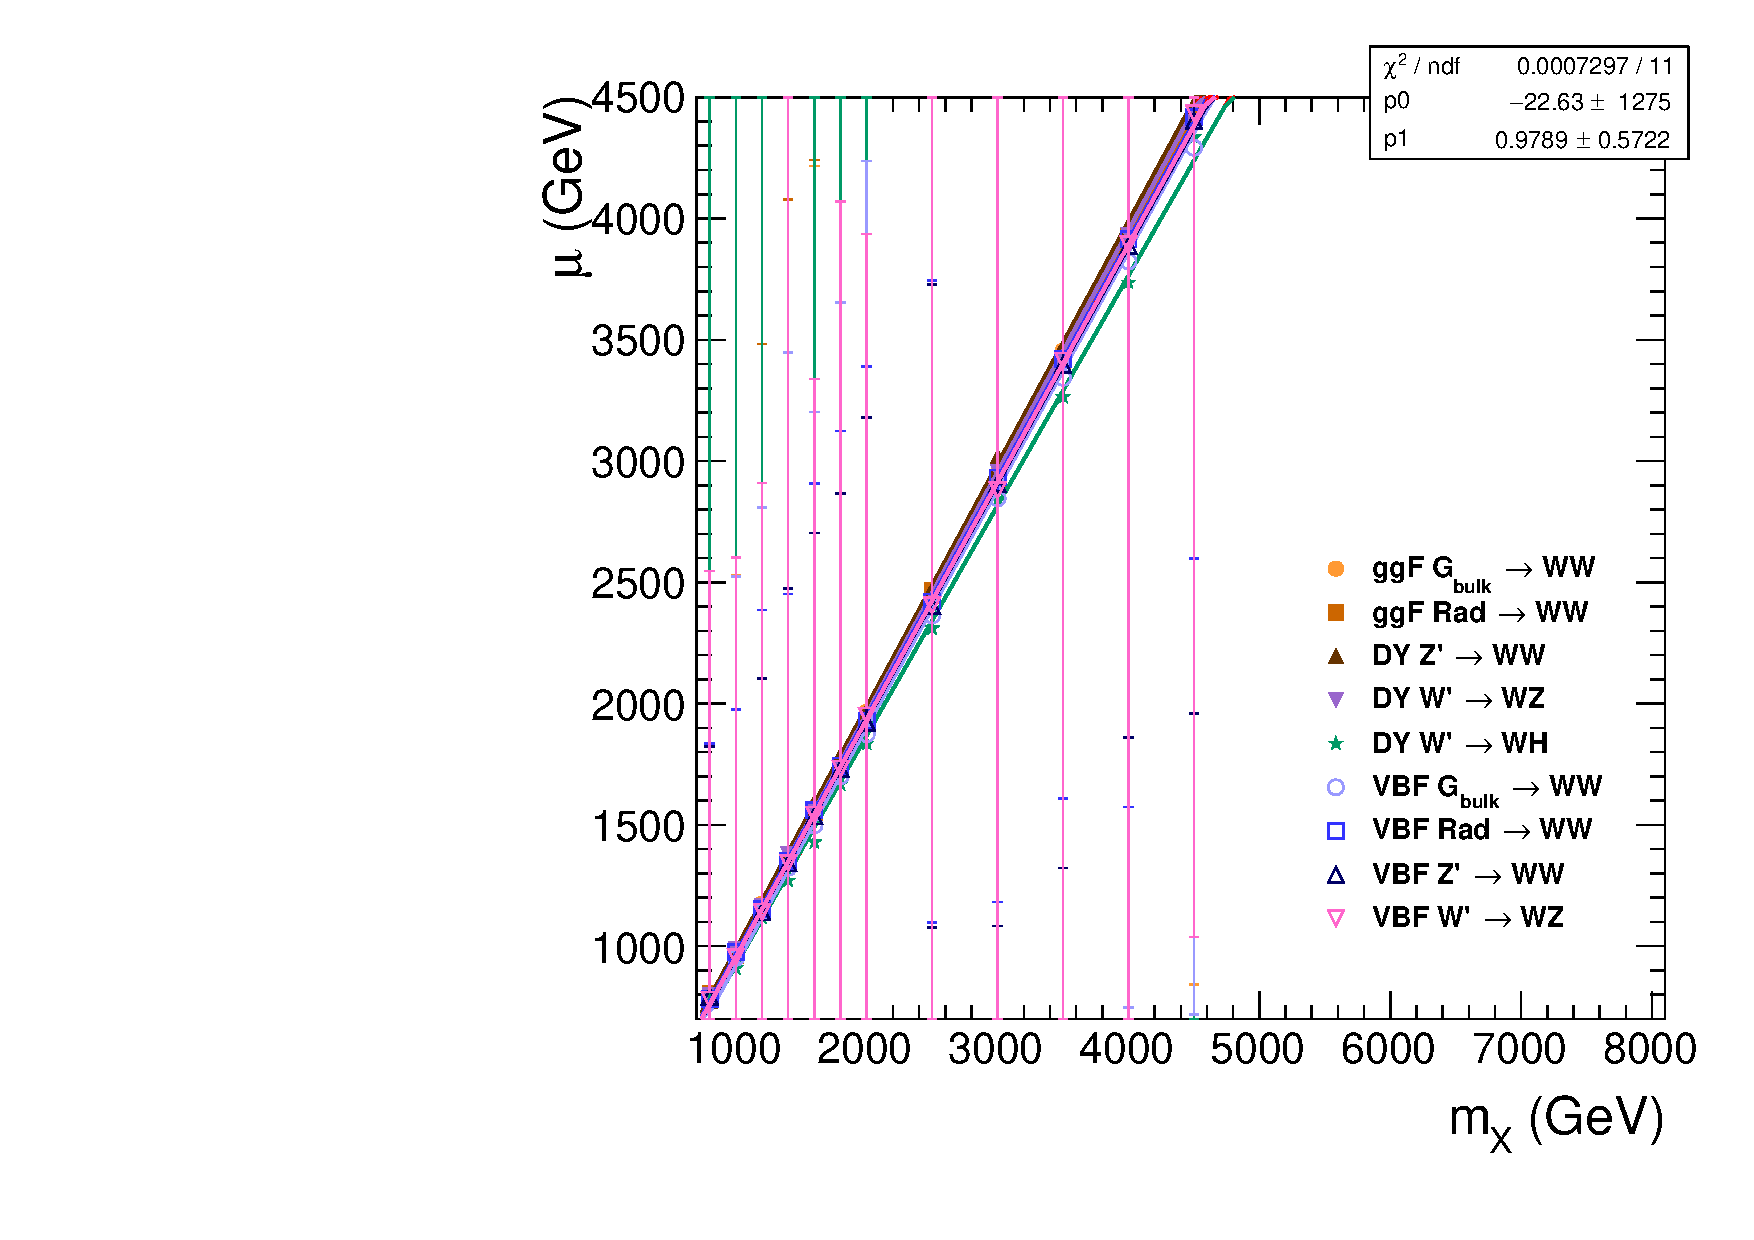
\includegraphics[width=0.2\textwidth]{fig/2Dfit/paramSignalShape_allSig_MVV_HP_vbf_HDy_MEAN.pdf}
  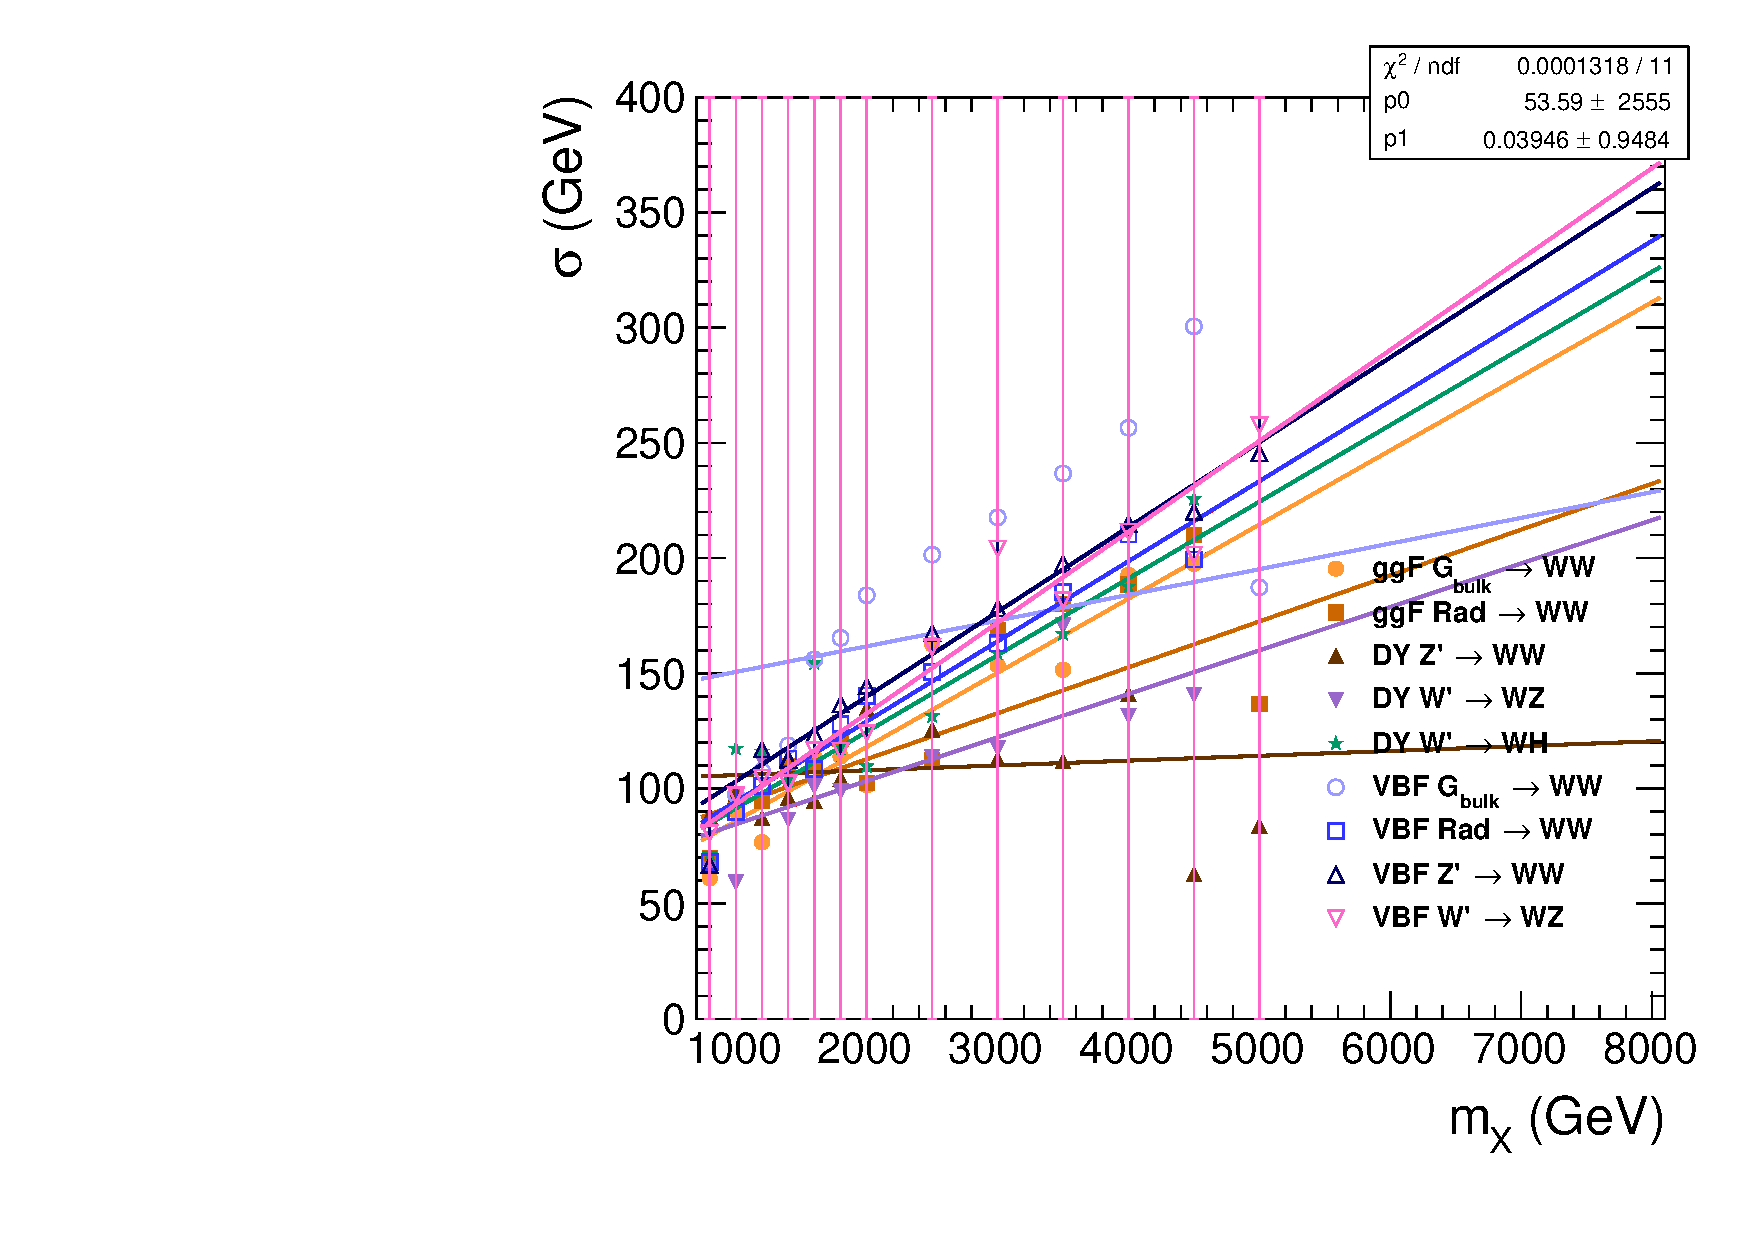
\includegraphics[width=0.2\textwidth]{fig/2Dfit/paramSignalShape_allSig_MVV_HP_vbf_HDy_SIGMA.pdf}
  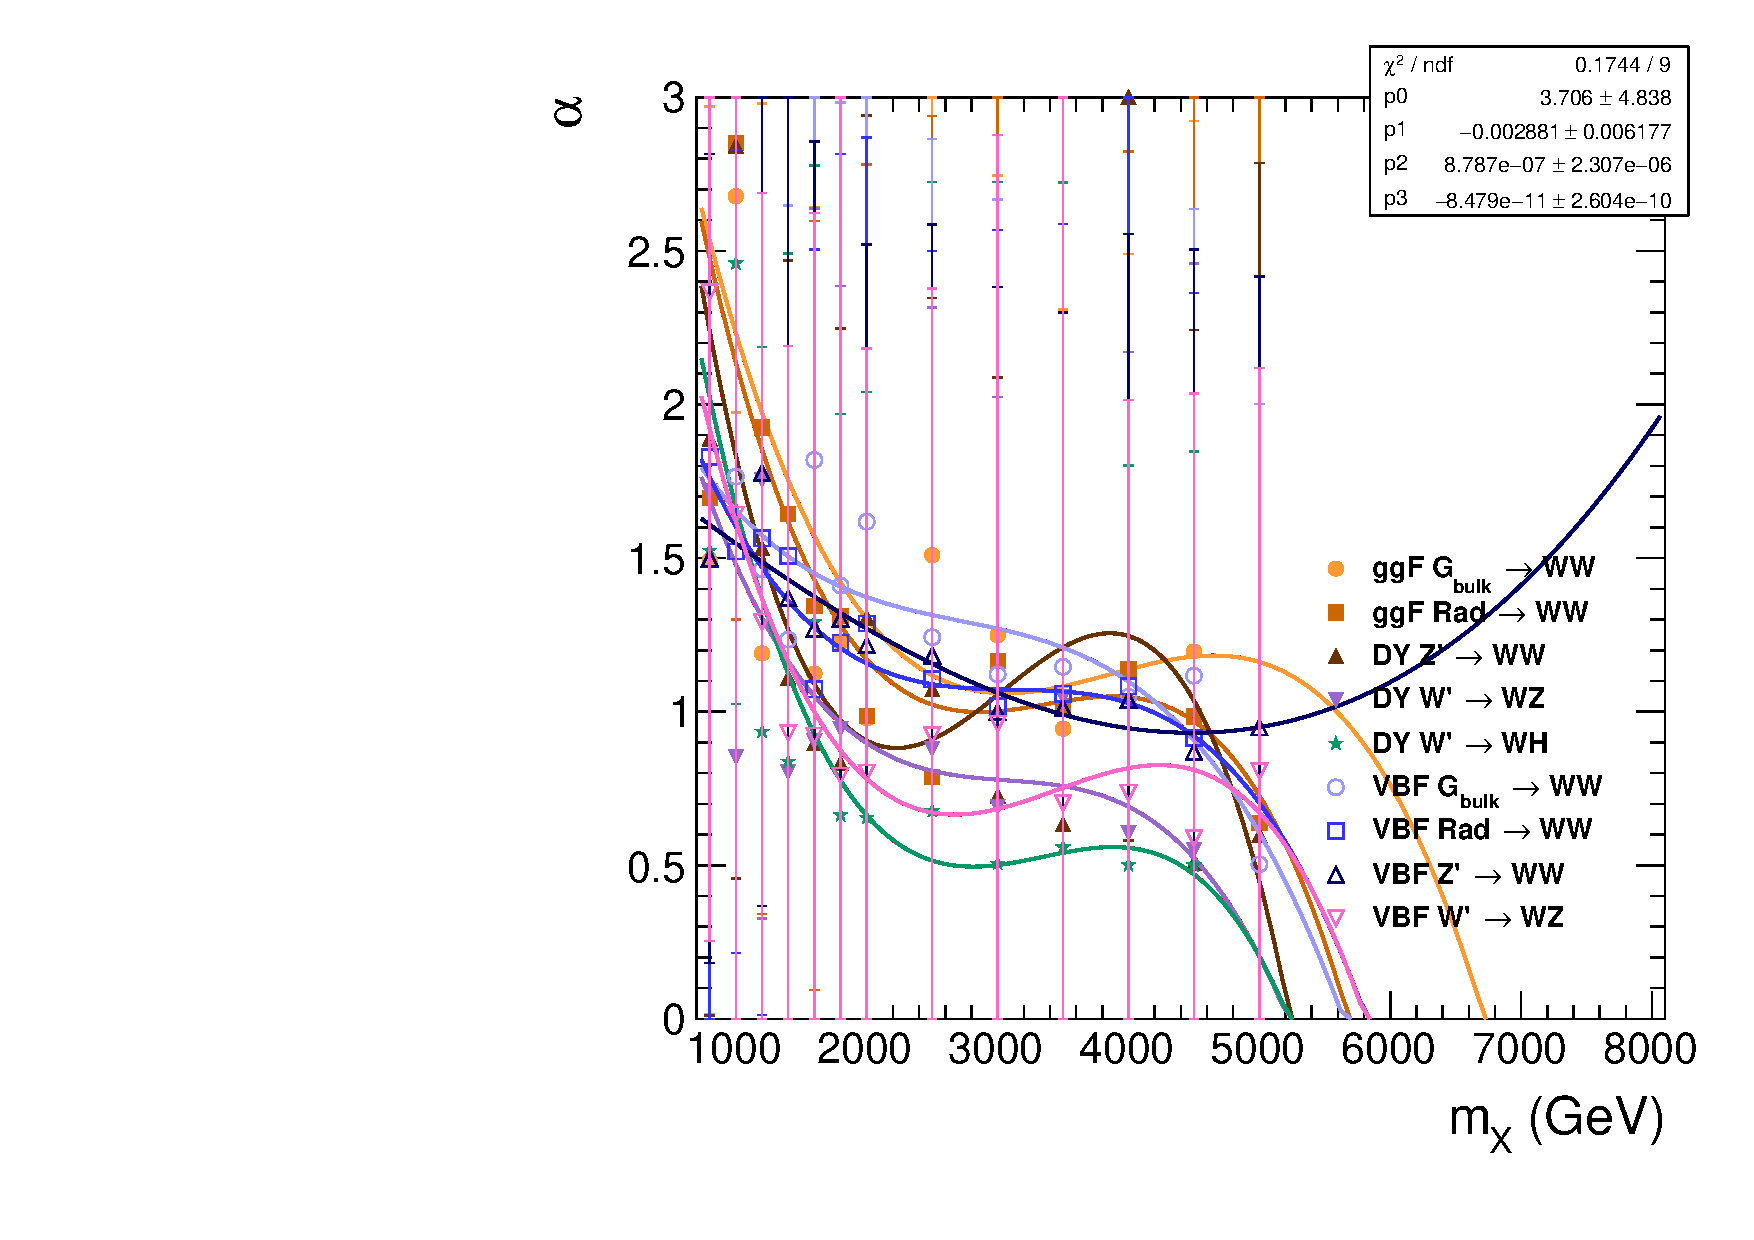
\includegraphics[width=0.2\textwidth]{fig/2Dfit/paramSignalShape_allSig_MVV_HP_vbf_HDy_ALPHA1.pdf}
  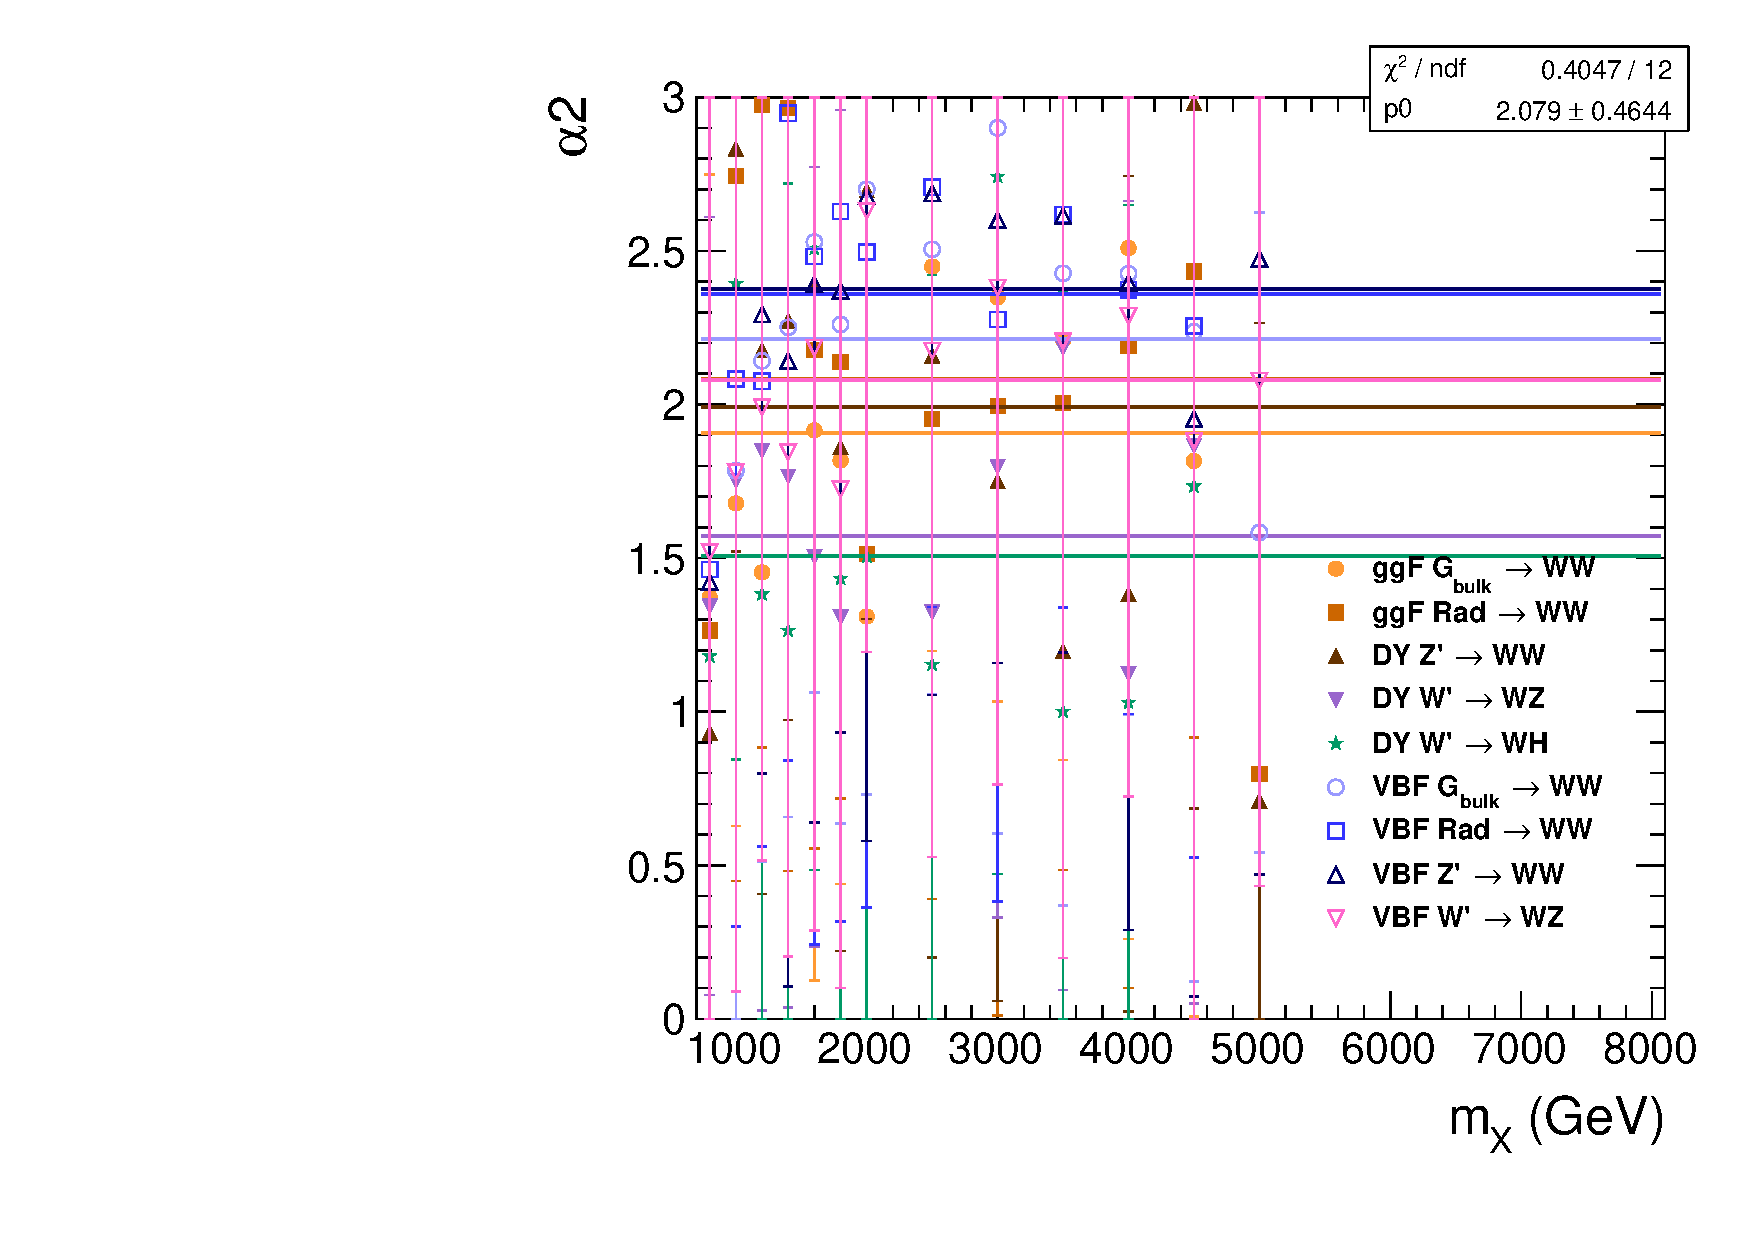
\includegraphics[width=0.2\textwidth]{fig/2Dfit/paramSignalShape_allSig_MVV_HP_vbf_HDy_ALPHA2.pdf}\\
  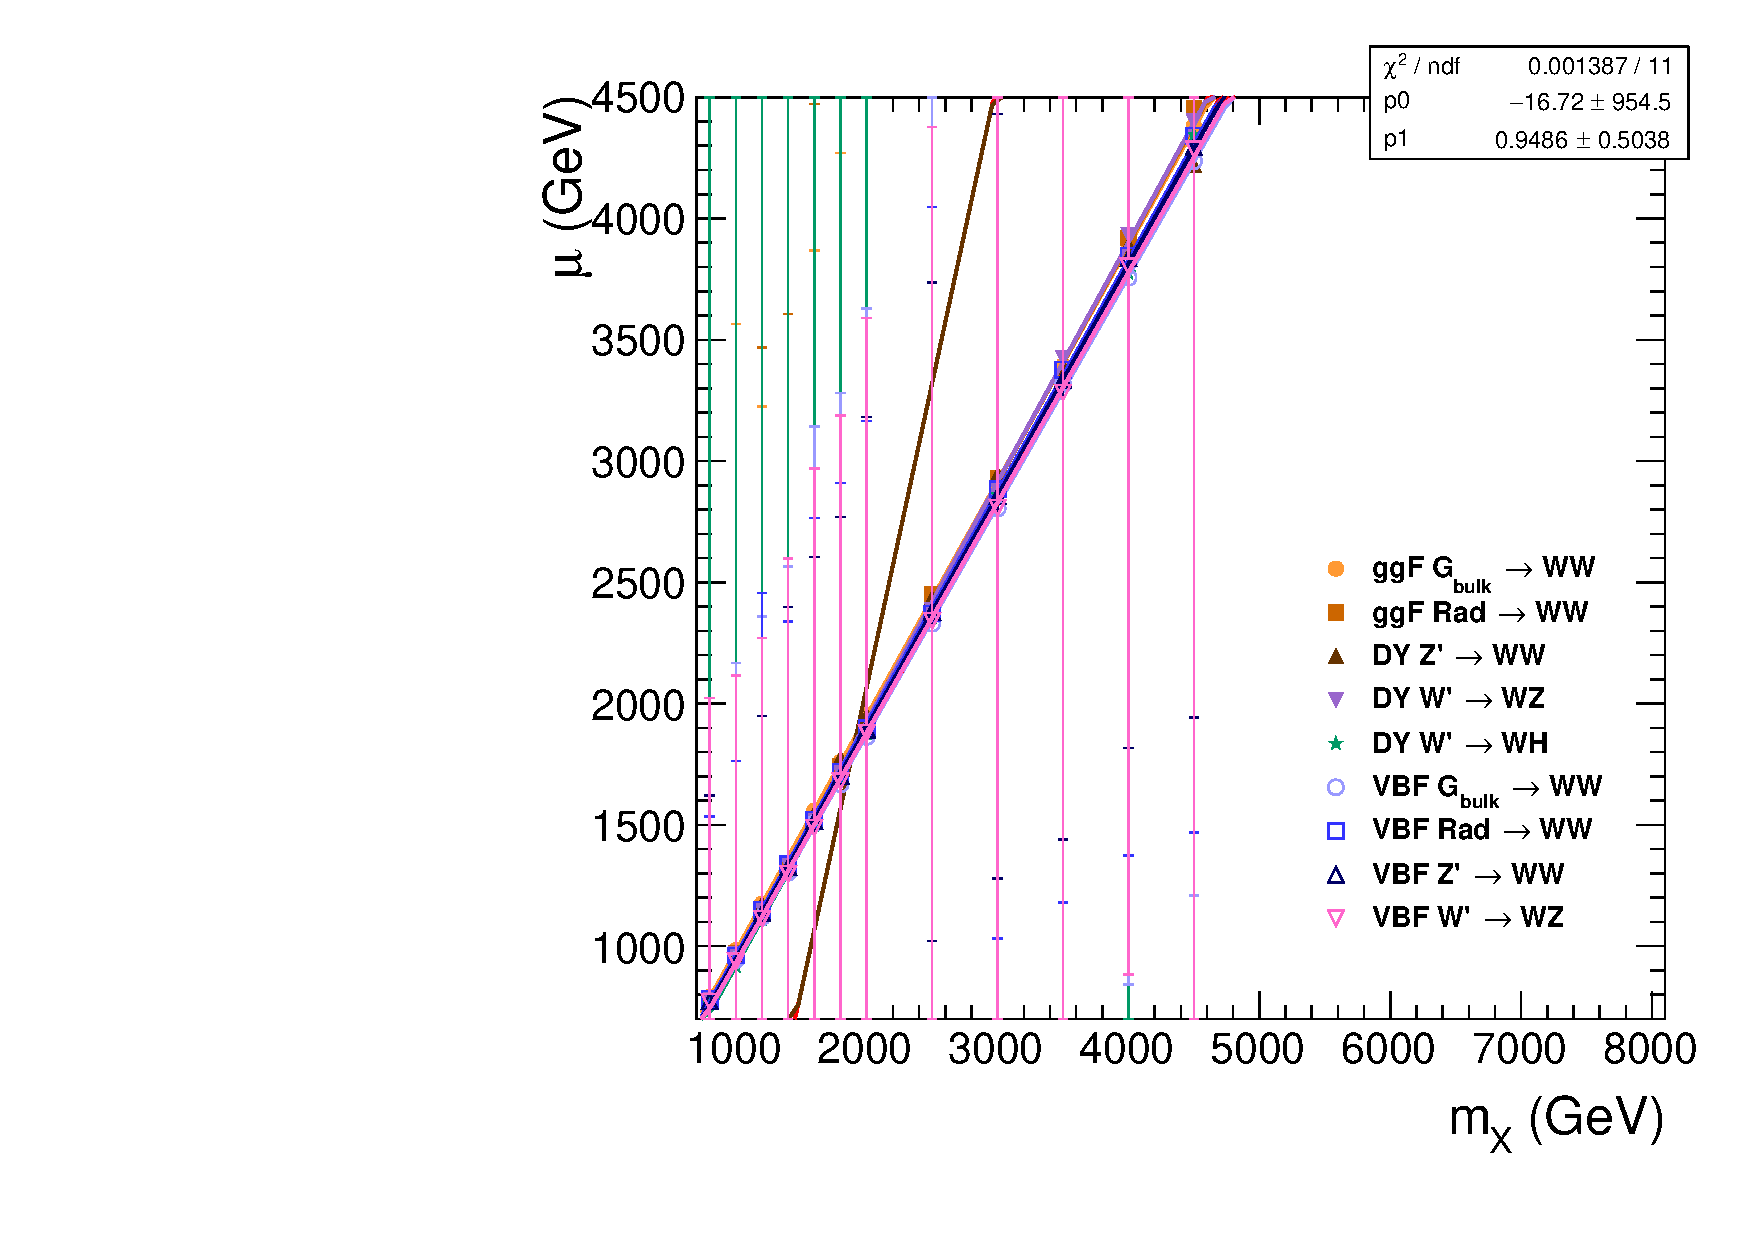
\includegraphics[width=0.2\textwidth]{fig/2Dfit/paramSignalShape_allSig_MVV_LP_vbf_HDy_MEAN.pdf}
  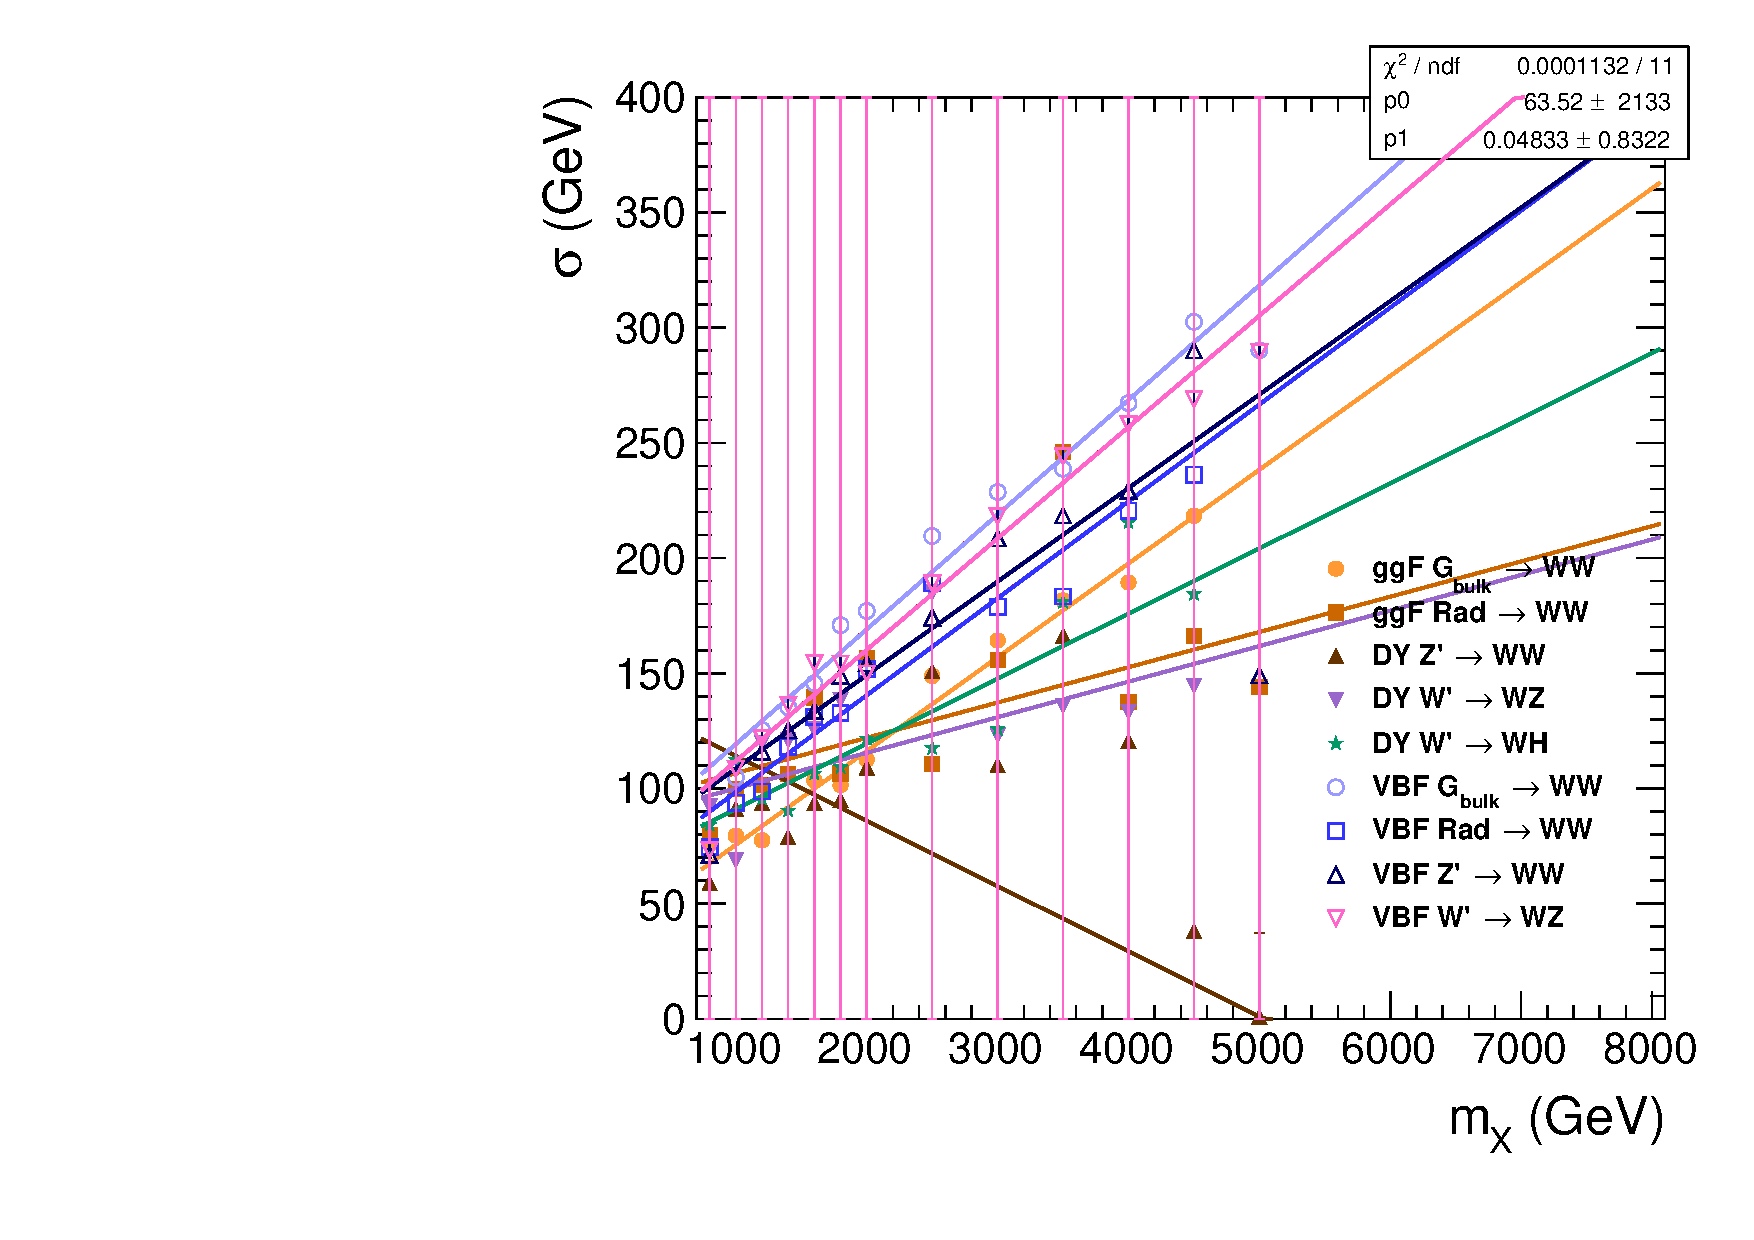
\includegraphics[width=0.2\textwidth]{fig/2Dfit/paramSignalShape_allSig_MVV_LP_vbf_HDy_SIGMA.pdf}
  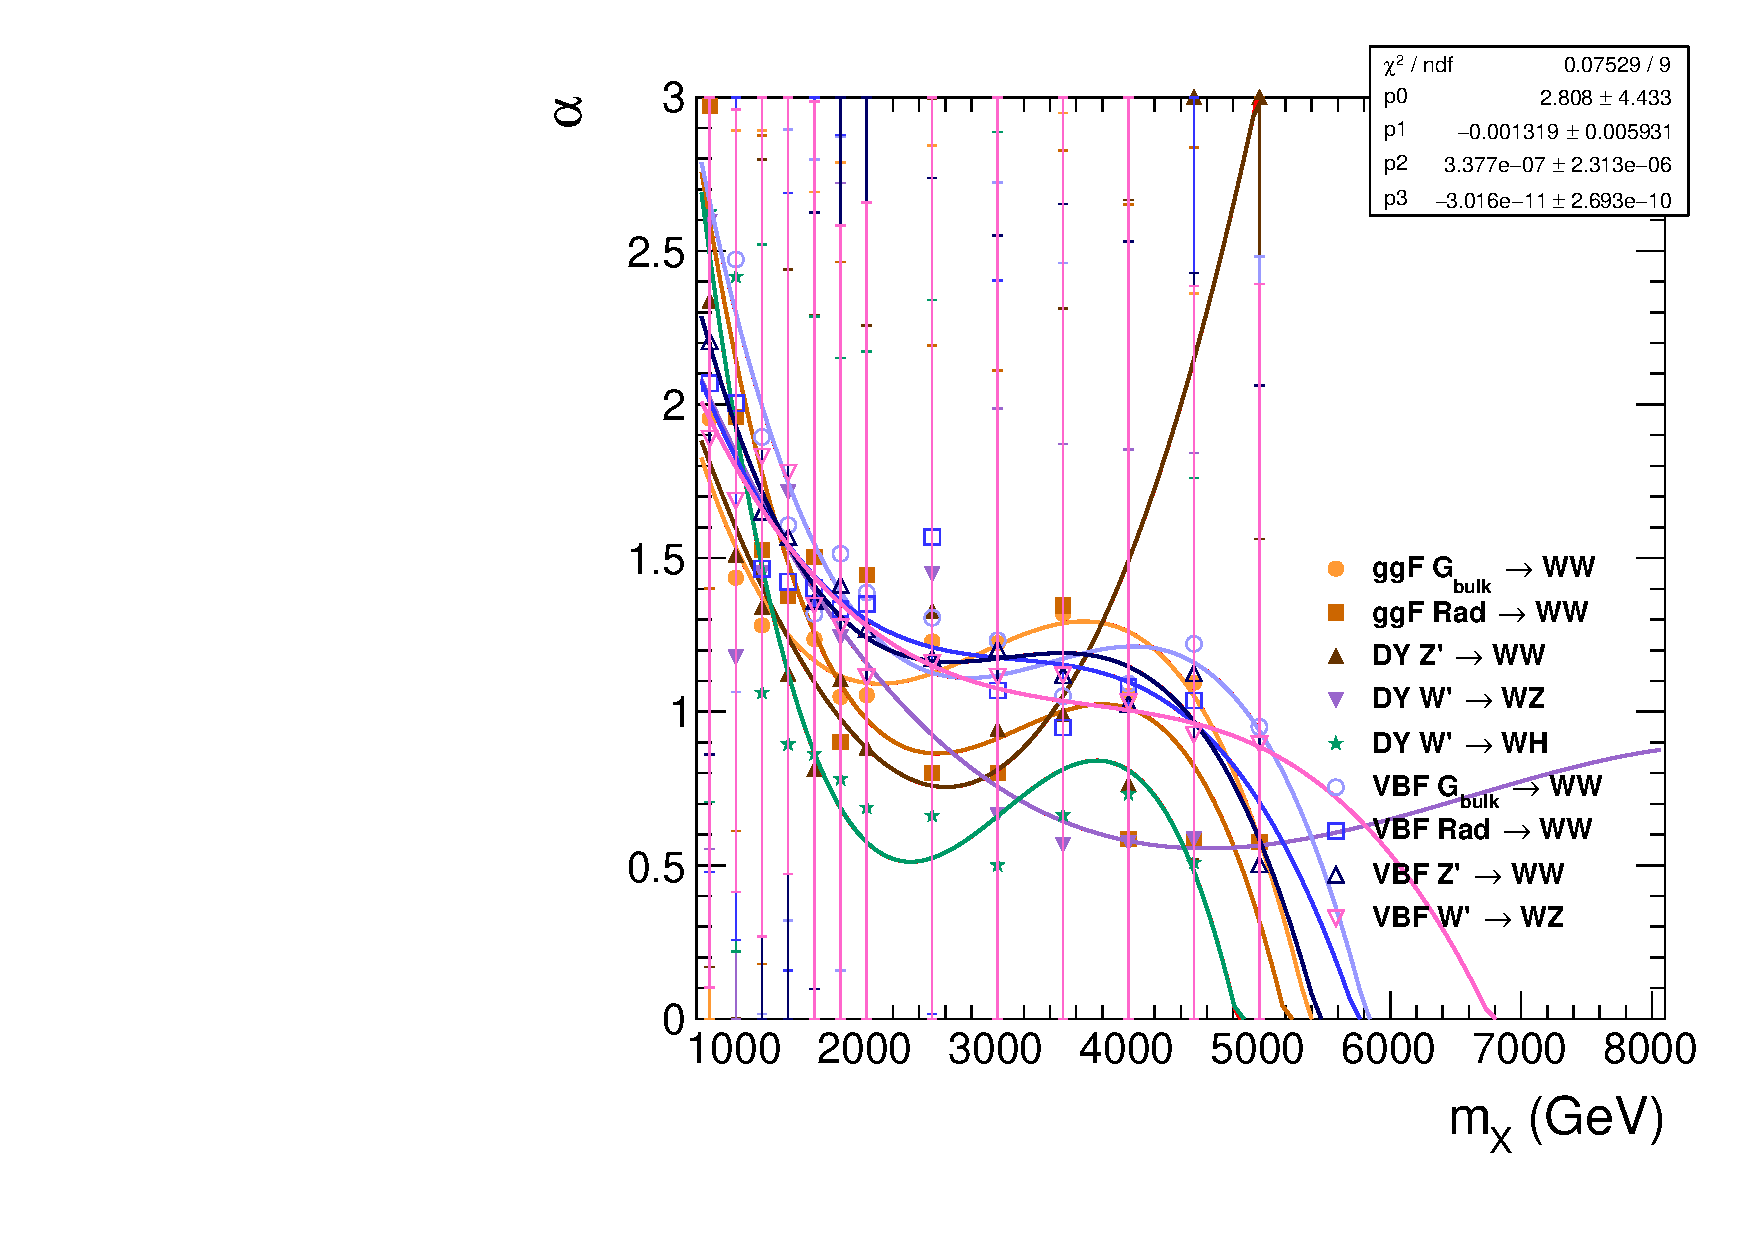
\includegraphics[width=0.2\textwidth]{fig/2Dfit/paramSignalShape_allSig_MVV_LP_vbf_HDy_ALPHA1.pdf}
  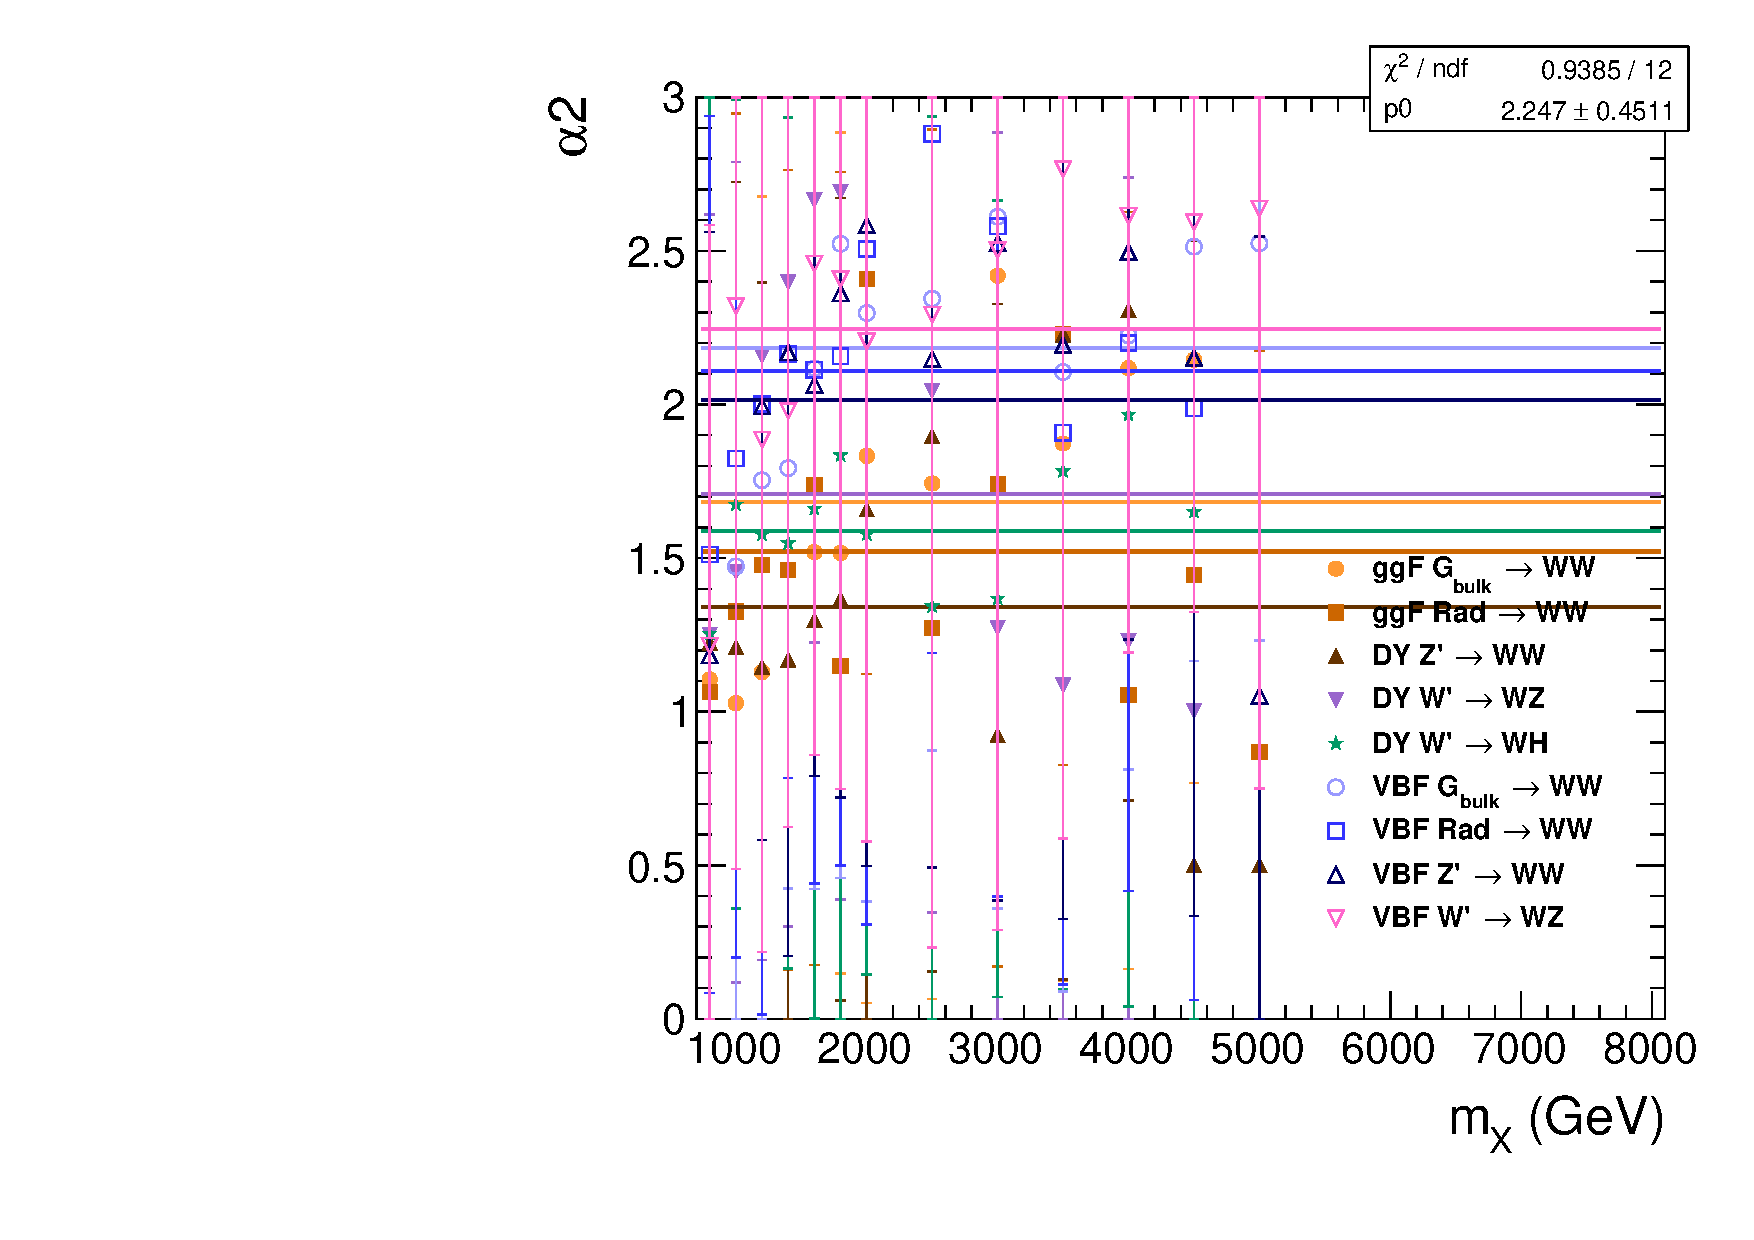
\includegraphics[width=0.2\textwidth]{fig/2Dfit/paramSignalShape_allSig_MVV_LP_vbf_HDy_ALPHA2.pdf}\\
  \caption{
    DCB parameters (from left to right: $\mu$, $\sigma$, $\alpha_1$, $\alpha_2$) for the diboson reconstructed mass \MVV as a function of \MX.
    Rows 1 to 6: HP-bb-HDy, LP-bb-HDy, HP-nobb-HDy, LP-nobb-HDy, HP-vbf-HDy, LP-vbf-HDy.
  }
  \label{fig:MVVShapeParam_HDy_Run2}
\end{figure}

\begin{figure}[htbp]
  \centering
  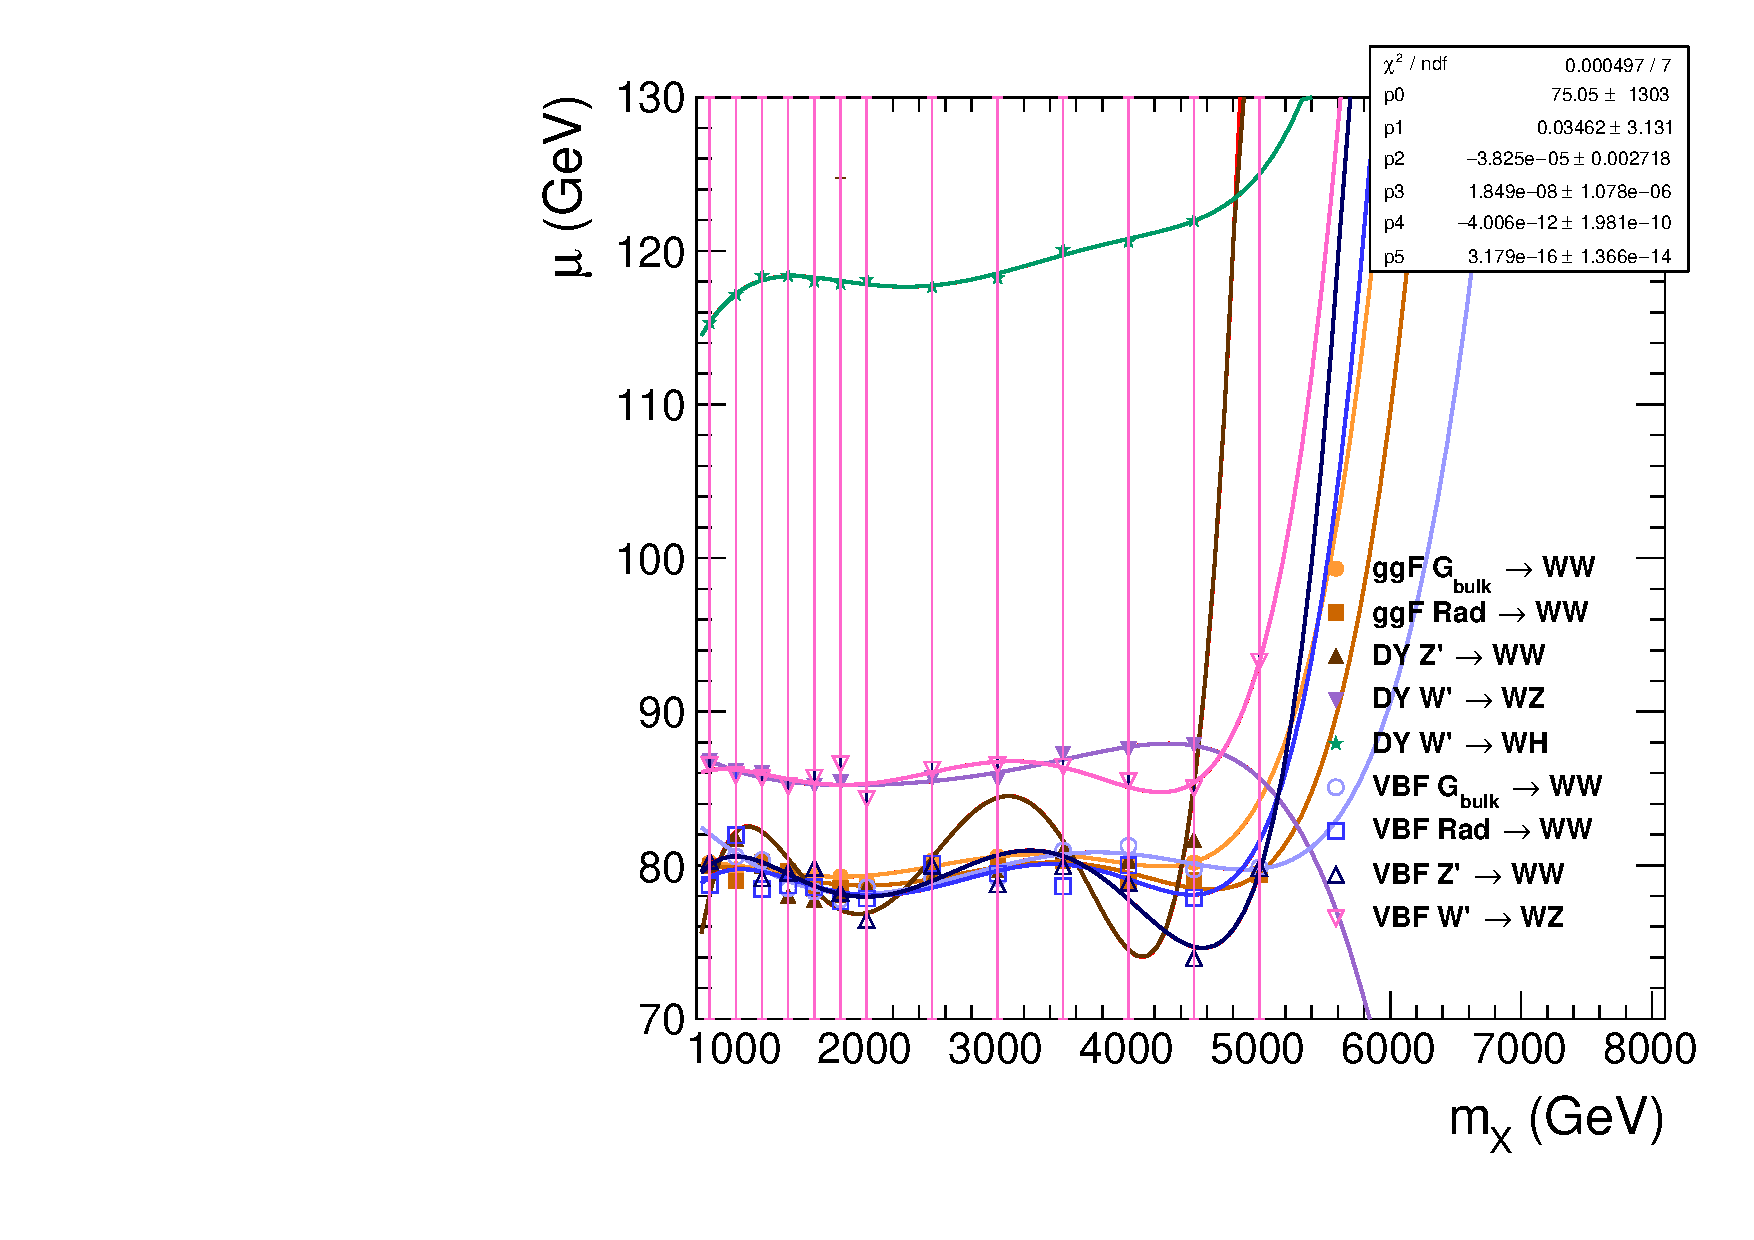
\includegraphics[width=0.2\textwidth]{fig/2Dfit/paramSignalShape_allSig_MJJ_HP_bb_LDy_mean.pdf}
  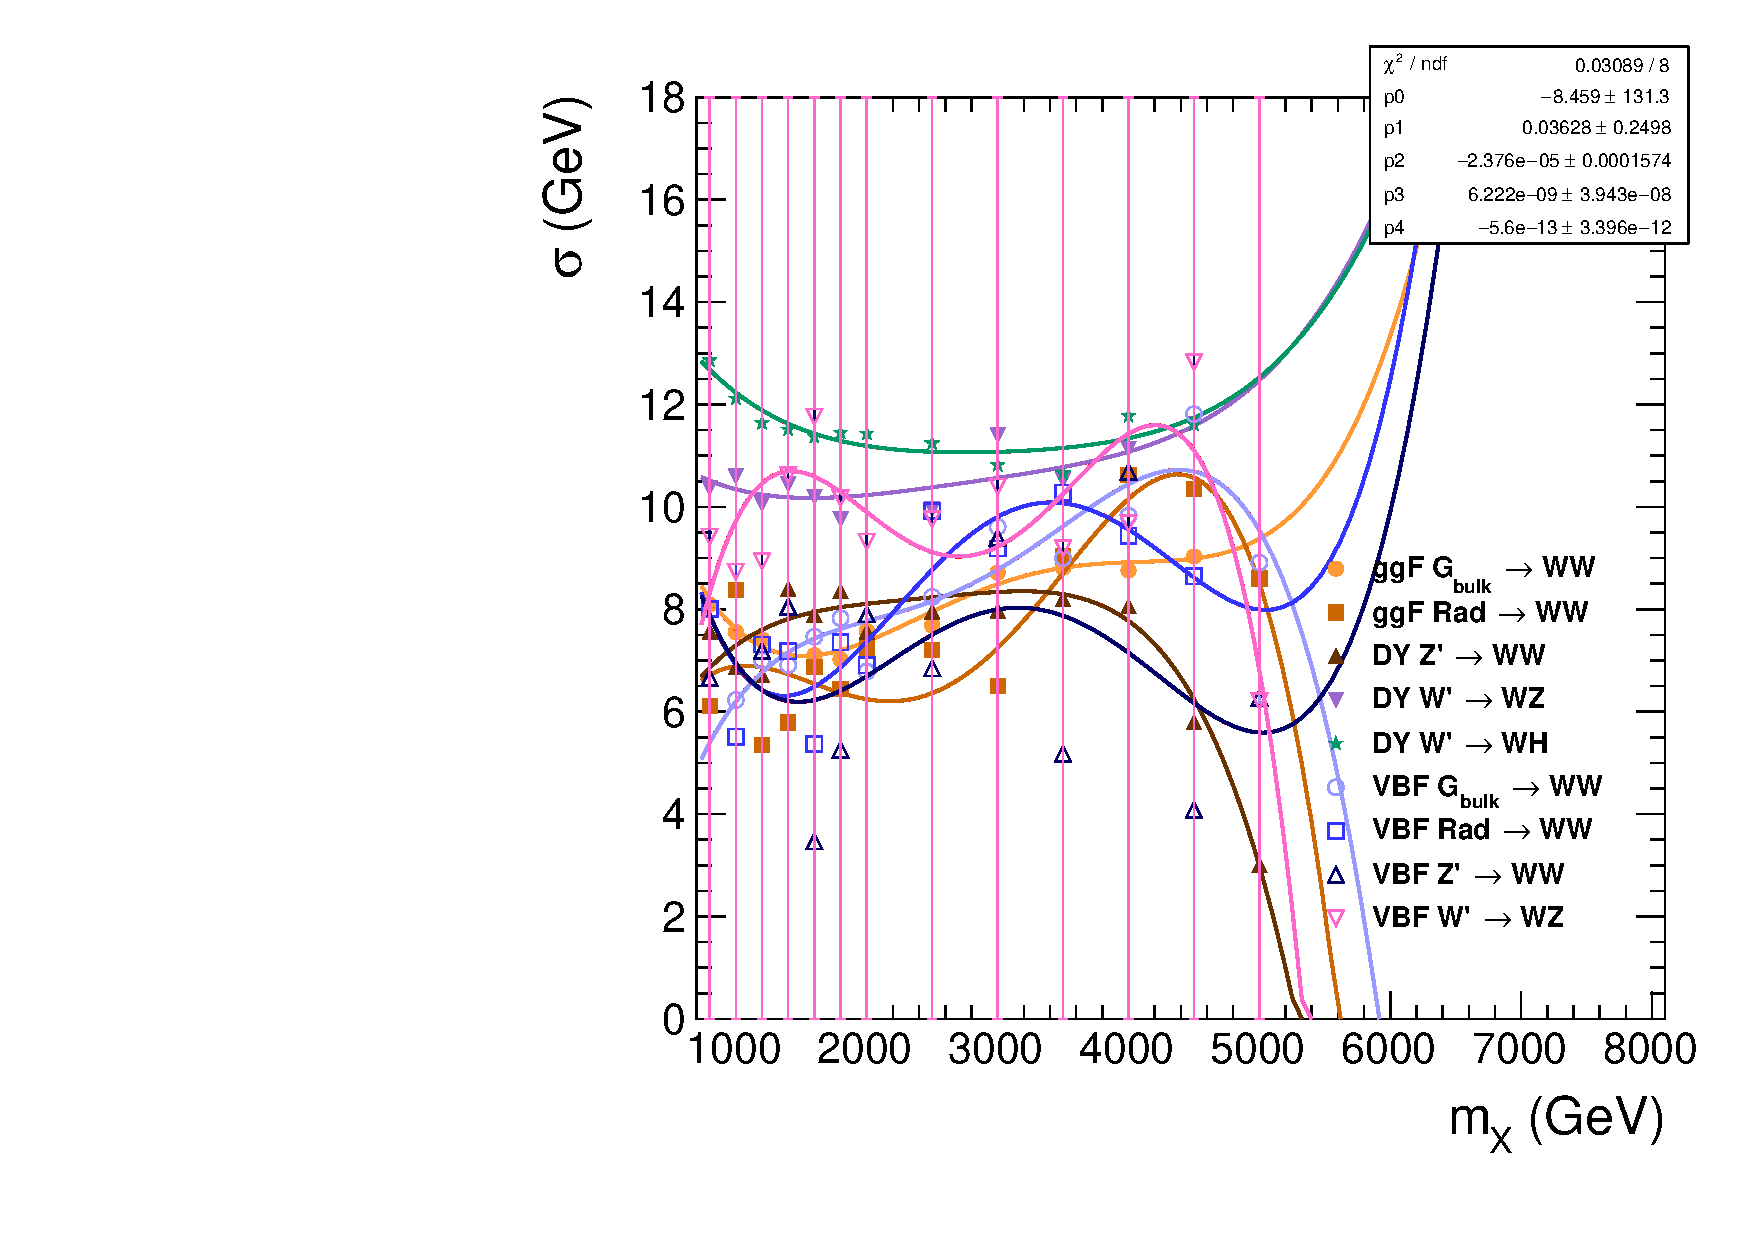
\includegraphics[width=0.2\textwidth]{fig/2Dfit/paramSignalShape_allSig_MJJ_HP_bb_LDy_sigma.pdf}
  \includegraphics[width=0.2\textwidth]{fig/2Dfit/paramSignalShape_allSig_MJJ_HP_bb_LDy_alpha.pdf}
  \includegraphics[width=0.2\textwidth]{fig/2Dfit/paramSignalShape_allSig_MJJ_HP_bb_LDy_alpha2.pdf}\\
  \includegraphics[width=0.2\textwidth]{fig/2Dfit/paramSignalShape_allSig_MJJ_LP_bb_LDy_mean.pdf}
  \includegraphics[width=0.2\textwidth]{fig/2Dfit/paramSignalShape_allSig_MJJ_LP_bb_LDy_sigma.pdf}
  \includegraphics[width=0.2\textwidth]{fig/2Dfit/paramSignalShape_allSig_MJJ_LP_bb_LDy_alpha.pdf}
  \includegraphics[width=0.2\textwidth]{fig/2Dfit/paramSignalShape_allSig_MJJ_LP_bb_LDy_alpha2.pdf}\\
  \includegraphics[width=0.2\textwidth]{fig/2Dfit/paramSignalShape_allSig_MJJ_HP_nobb_LDy_mean.pdf}
  \includegraphics[width=0.2\textwidth]{fig/2Dfit/paramSignalShape_allSig_MJJ_HP_nobb_LDy_sigma.pdf}
  \includegraphics[width=0.2\textwidth]{fig/2Dfit/paramSignalShape_allSig_MJJ_HP_nobb_LDy_alpha.pdf}
  \includegraphics[width=0.2\textwidth]{fig/2Dfit/paramSignalShape_allSig_MJJ_HP_nobb_LDy_alpha2.pdf}\\
  \includegraphics[width=0.2\textwidth]{fig/2Dfit/paramSignalShape_allSig_MJJ_LP_nobb_LDy_mean.pdf}
  \includegraphics[width=0.2\textwidth]{fig/2Dfit/paramSignalShape_allSig_MJJ_LP_nobb_LDy_sigma.pdf}
  \includegraphics[width=0.2\textwidth]{fig/2Dfit/paramSignalShape_allSig_MJJ_LP_nobb_LDy_alpha.pdf}
  \includegraphics[width=0.2\textwidth]{fig/2Dfit/paramSignalShape_allSig_MJJ_LP_nobb_LDy_alpha2.pdf}\\
  \includegraphics[width=0.2\textwidth]{fig/2Dfit/paramSignalShape_allSig_MJJ_HP_vbf_LDy_mean.pdf}
  \includegraphics[width=0.2\textwidth]{fig/2Dfit/paramSignalShape_allSig_MJJ_HP_vbf_LDy_sigma.pdf}
  \includegraphics[width=0.2\textwidth]{fig/2Dfit/paramSignalShape_allSig_MJJ_HP_vbf_LDy_alpha.pdf}
  \includegraphics[width=0.2\textwidth]{fig/2Dfit/paramSignalShape_allSig_MJJ_HP_vbf_LDy_alpha2.pdf}\\
  \includegraphics[width=0.2\textwidth]{fig/2Dfit/paramSignalShape_allSig_MJJ_LP_vbf_LDy_mean.pdf}
  \includegraphics[width=0.2\textwidth]{fig/2Dfit/paramSignalShape_allSig_MJJ_LP_vbf_LDy_sigma.pdf}
  \includegraphics[width=0.2\textwidth]{fig/2Dfit/paramSignalShape_allSig_MJJ_LP_vbf_LDy_alpha.pdf}
  \includegraphics[width=0.2\textwidth]{fig/2Dfit/paramSignalShape_allSig_MJJ_LP_vbf_LDy_alpha2.pdf}\\
  \caption{
    DCB parameters (from left to right: $\mu$, $\sigma$, $\alpha_1$, $\alpha_2$) for the jet mass \MJ as a function of \MX.
    Rows 1 to 6: HP-bb-LDy, LP-bb-LDy, HP-nobb-LDy, LP-nobb-LDy, HP-vbf-LDy, LP-vbf-LDy.
  }
  \label{fig:MJJShapeParam_LDy_Run2}
\end{figure}

\begin{figure}[htbp]
  \centering
  \includegraphics[width=0.2\textwidth]{fig/2Dfit/paramSignalShape_allSig_MJJ_HP_bb_HDy_mean.pdf}
  \includegraphics[width=0.2\textwidth]{fig/2Dfit/paramSignalShape_allSig_MJJ_HP_bb_HDy_sigma.pdf}
  \includegraphics[width=0.2\textwidth]{fig/2Dfit/paramSignalShape_allSig_MJJ_HP_bb_HDy_alpha.pdf}
  \includegraphics[width=0.2\textwidth]{fig/2Dfit/paramSignalShape_allSig_MJJ_HP_bb_HDy_alpha2.pdf}\\
  \includegraphics[width=0.2\textwidth]{fig/2Dfit/paramSignalShape_allSig_MJJ_LP_bb_HDy_mean.pdf}
  \includegraphics[width=0.2\textwidth]{fig/2Dfit/paramSignalShape_allSig_MJJ_LP_bb_HDy_sigma.pdf}
  \includegraphics[width=0.2\textwidth]{fig/2Dfit/paramSignalShape_allSig_MJJ_LP_bb_HDy_alpha.pdf}
  \includegraphics[width=0.2\textwidth]{fig/2Dfit/paramSignalShape_allSig_MJJ_LP_bb_HDy_alpha2.pdf}\\
  \includegraphics[width=0.2\textwidth]{fig/2Dfit/paramSignalShape_allSig_MJJ_HP_nobb_HDy_mean.pdf}
  \includegraphics[width=0.2\textwidth]{fig/2Dfit/paramSignalShape_allSig_MJJ_HP_nobb_HDy_sigma.pdf}
  \includegraphics[width=0.2\textwidth]{fig/2Dfit/paramSignalShape_allSig_MJJ_HP_nobb_HDy_alpha.pdf}
  \includegraphics[width=0.2\textwidth]{fig/2Dfit/paramSignalShape_allSig_MJJ_HP_nobb_HDy_alpha2.pdf}\\
  \includegraphics[width=0.2\textwidth]{fig/2Dfit/paramSignalShape_allSig_MJJ_LP_nobb_HDy_mean.pdf}
  \includegraphics[width=0.2\textwidth]{fig/2Dfit/paramSignalShape_allSig_MJJ_LP_nobb_HDy_sigma.pdf}
  \includegraphics[width=0.2\textwidth]{fig/2Dfit/paramSignalShape_allSig_MJJ_LP_nobb_HDy_alpha.pdf}
  \includegraphics[width=0.2\textwidth]{fig/2Dfit/paramSignalShape_allSig_MJJ_LP_nobb_HDy_alpha2.pdf}\\
  \includegraphics[width=0.2\textwidth]{fig/2Dfit/paramSignalShape_allSig_MJJ_HP_vbf_HDy_mean.pdf}
  \includegraphics[width=0.2\textwidth]{fig/2Dfit/paramSignalShape_allSig_MJJ_HP_vbf_HDy_sigma.pdf}
  \includegraphics[width=0.2\textwidth]{fig/2Dfit/paramSignalShape_allSig_MJJ_HP_vbf_HDy_alpha.pdf}
  \includegraphics[width=0.2\textwidth]{fig/2Dfit/paramSignalShape_allSig_MJJ_HP_vbf_HDy_alpha2.pdf}\\
  \includegraphics[width=0.2\textwidth]{fig/2Dfit/paramSignalShape_allSig_MJJ_LP_vbf_HDy_mean.pdf}
  \includegraphics[width=0.2\textwidth]{fig/2Dfit/paramSignalShape_allSig_MJJ_LP_vbf_HDy_sigma.pdf}
  \includegraphics[width=0.2\textwidth]{fig/2Dfit/paramSignalShape_allSig_MJJ_LP_vbf_HDy_alpha.pdf}
  \includegraphics[width=0.2\textwidth]{fig/2Dfit/paramSignalShape_allSig_MJJ_LP_vbf_HDy_alpha2.pdf}\\
  \caption{
    DCB parameters (from left to right: $\mu$, $\sigma$, $\alpha_1$, $\alpha_2$) for the jet mass \MJ as a function of \MX.
    Rows 1 to 6: HP-bb-HDy, LP-bb-HDy, HP-nobb-HDy, LP-nobb-HDy, HP-vbf-HDy, LP-vbf-HDy.
  }
  \label{fig:MJJShapeParam_HDy_Run2}
\end{figure}

\begin{figure}[htbp]
  \centering
  \includegraphics[width=0.18\textwidth]{fig/2Dfit/templateSignalVsMX_fromDC_GbuToWW_MVV_mu_HP_bb_LDy.pdf}
  \includegraphics[width=0.18\textwidth]{fig/2Dfit/templateSignalVsMX_fromDC_RadToWW_MVV_mu_HP_bb_LDy.pdf}
  \includegraphics[width=0.18\textwidth]{fig/2Dfit/templateSignalVsMX_fromDC_ZprToWW_MVV_mu_HP_bb_LDy.pdf}
  \includegraphics[width=0.18\textwidth]{fig/2Dfit/templateSignalVsMX_fromDC_WprToWZ_MVV_mu_HP_bb_LDy.pdf}
  \includegraphics[width=0.18\textwidth]{fig/2Dfit/templateSignalVsMX_fromDC_WprToWH_MVV_mu_HP_bb_LDy.pdf}\\
  \includegraphics[width=0.18\textwidth]{fig/2Dfit/templateSignalVsMX_fromDC_GbuToWW_MVV_mu_LP_bb_LDy.pdf}
  \includegraphics[width=0.18\textwidth]{fig/2Dfit/templateSignalVsMX_fromDC_RadToWW_MVV_mu_LP_bb_LDy.pdf}
  \includegraphics[width=0.18\textwidth]{fig/2Dfit/templateSignalVsMX_fromDC_ZprToWW_MVV_mu_LP_bb_LDy.pdf}
  \includegraphics[width=0.18\textwidth]{fig/2Dfit/templateSignalVsMX_fromDC_WprToWZ_MVV_mu_LP_bb_LDy.pdf}
  \includegraphics[width=0.18\textwidth]{fig/2Dfit/templateSignalVsMX_fromDC_WprToWH_MVV_mu_LP_bb_LDy.pdf}\\
  \includegraphics[width=0.18\textwidth]{fig/2Dfit/templateSignalVsMX_fromDC_GbuToWW_MVV_mu_HP_nobb_LDy.pdf}
  \includegraphics[width=0.18\textwidth]{fig/2Dfit/templateSignalVsMX_fromDC_RadToWW_MVV_mu_HP_nobb_LDy.pdf}
  \includegraphics[width=0.18\textwidth]{fig/2Dfit/templateSignalVsMX_fromDC_ZprToWW_MVV_mu_HP_nobb_LDy.pdf}
  \includegraphics[width=0.18\textwidth]{fig/2Dfit/templateSignalVsMX_fromDC_WprToWZ_MVV_mu_HP_nobb_LDy.pdf}
  \includegraphics[width=0.18\textwidth]{fig/2Dfit/templateSignalVsMX_fromDC_WprToWH_MVV_mu_HP_nobb_LDy.pdf}\\
  \includegraphics[width=0.18\textwidth]{fig/2Dfit/templateSignalVsMX_fromDC_GbuToWW_MVV_mu_LP_nobb_LDy.pdf}
  \includegraphics[width=0.18\textwidth]{fig/2Dfit/templateSignalVsMX_fromDC_RadToWW_MVV_mu_LP_nobb_LDy.pdf}
  \includegraphics[width=0.18\textwidth]{fig/2Dfit/templateSignalVsMX_fromDC_ZprToWW_MVV_mu_LP_nobb_LDy.pdf}
  \includegraphics[width=0.18\textwidth]{fig/2Dfit/templateSignalVsMX_fromDC_WprToWZ_MVV_mu_LP_nobb_LDy.pdf}
  \includegraphics[width=0.18\textwidth]{fig/2Dfit/templateSignalVsMX_fromDC_WprToWH_MVV_mu_LP_nobb_LDy.pdf}\\
  \includegraphics[width=0.18\textwidth]{fig/2Dfit/templateSignalVsMX_fromDC_GbuToWW_MVV_mu_HP_vbf_LDy.pdf}
  \includegraphics[width=0.18\textwidth]{fig/2Dfit/templateSignalVsMX_fromDC_RadToWW_MVV_mu_HP_vbf_LDy.pdf}
  \includegraphics[width=0.18\textwidth]{fig/2Dfit/templateSignalVsMX_fromDC_ZprToWW_MVV_mu_HP_vbf_LDy.pdf}
  \includegraphics[width=0.18\textwidth]{fig/2Dfit/templateSignalVsMX_fromDC_WprToWZ_MVV_mu_HP_vbf_LDy.pdf}
  \includegraphics[width=0.18\textwidth]{fig/2Dfit/templateSignalVsMX_fromDC_WprToWH_MVV_mu_HP_vbf_LDy.pdf}\\
  \includegraphics[width=0.18\textwidth]{fig/2Dfit/templateSignalVsMX_fromDC_GbuToWW_MVV_mu_LP_vbf_LDy.pdf}
  \includegraphics[width=0.18\textwidth]{fig/2Dfit/templateSignalVsMX_fromDC_RadToWW_MVV_mu_LP_vbf_LDy.pdf}
  \includegraphics[width=0.18\textwidth]{fig/2Dfit/templateSignalVsMX_fromDC_ZprToWW_MVV_mu_LP_vbf_LDy.pdf}
  \includegraphics[width=0.18\textwidth]{fig/2Dfit/templateSignalVsMX_fromDC_WprToWZ_MVV_mu_LP_vbf_LDy.pdf}
  \includegraphics[width=0.18\textwidth]{fig/2Dfit/templateSignalVsMX_fromDC_WprToWH_MVV_mu_LP_vbf_LDy.pdf}\\
  \caption{
    Signal shapes for the diboson reconstructed mass \MVV for \ggF- and \DY-produced signals, for 8 values of \MX.
    From left to right: \GBulktoWW, \RadtoWW, \ZprtoWW, \WprtoWZ, \WprtoWH.
    Rows 1 to 6: HP-bb-LDy, LP-bb-LDy, HP-nobb-LDy, LP-nobb-LDy, HP-vbf-LDy, LP-vbf-LDy.
  }
  \label{fig:MVVShapes_NonVBF_LDy_Run2}
\end{figure}

\begin{figure}[htbp]
  \centering
  \includegraphics[width=0.18\textwidth]{fig/2Dfit/templateSignalVsMX_fromDC_GbuToWW_MVV_mu_HP_bb_HDy.pdf}
  \includegraphics[width=0.18\textwidth]{fig/2Dfit/templateSignalVsMX_fromDC_RadToWW_MVV_mu_HP_bb_HDy.pdf}
  \includegraphics[width=0.18\textwidth]{fig/2Dfit/templateSignalVsMX_fromDC_ZprToWW_MVV_mu_HP_bb_HDy.pdf}
  \includegraphics[width=0.18\textwidth]{fig/2Dfit/templateSignalVsMX_fromDC_WprToWZ_MVV_mu_HP_bb_HDy.pdf}
  \includegraphics[width=0.18\textwidth]{fig/2Dfit/templateSignalVsMX_fromDC_WprToWH_MVV_mu_HP_bb_HDy.pdf}\\
  \includegraphics[width=0.18\textwidth]{fig/2Dfit/templateSignalVsMX_fromDC_GbuToWW_MVV_mu_LP_bb_HDy.pdf}
  \includegraphics[width=0.18\textwidth]{fig/2Dfit/templateSignalVsMX_fromDC_RadToWW_MVV_mu_LP_bb_HDy.pdf}
  \includegraphics[width=0.18\textwidth]{fig/2Dfit/templateSignalVsMX_fromDC_ZprToWW_MVV_mu_LP_bb_HDy.pdf}
  \includegraphics[width=0.18\textwidth]{fig/2Dfit/templateSignalVsMX_fromDC_WprToWZ_MVV_mu_LP_bb_HDy.pdf}
  \includegraphics[width=0.18\textwidth]{fig/2Dfit/templateSignalVsMX_fromDC_WprToWH_MVV_mu_LP_bb_HDy.pdf}\\
  \includegraphics[width=0.18\textwidth]{fig/2Dfit/templateSignalVsMX_fromDC_GbuToWW_MVV_mu_HP_nobb_HDy.pdf}
  \includegraphics[width=0.18\textwidth]{fig/2Dfit/templateSignalVsMX_fromDC_RadToWW_MVV_mu_HP_nobb_HDy.pdf}
  \includegraphics[width=0.18\textwidth]{fig/2Dfit/templateSignalVsMX_fromDC_ZprToWW_MVV_mu_HP_nobb_HDy.pdf}
  \includegraphics[width=0.18\textwidth]{fig/2Dfit/templateSignalVsMX_fromDC_WprToWZ_MVV_mu_HP_nobb_HDy.pdf}
  \includegraphics[width=0.18\textwidth]{fig/2Dfit/templateSignalVsMX_fromDC_WprToWH_MVV_mu_HP_nobb_HDy.pdf}\\
  \includegraphics[width=0.18\textwidth]{fig/2Dfit/templateSignalVsMX_fromDC_GbuToWW_MVV_mu_LP_nobb_HDy.pdf}
  \includegraphics[width=0.18\textwidth]{fig/2Dfit/templateSignalVsMX_fromDC_RadToWW_MVV_mu_LP_nobb_HDy.pdf}
  \includegraphics[width=0.18\textwidth]{fig/2Dfit/templateSignalVsMX_fromDC_ZprToWW_MVV_mu_LP_nobb_HDy.pdf}
  \includegraphics[width=0.18\textwidth]{fig/2Dfit/templateSignalVsMX_fromDC_WprToWZ_MVV_mu_LP_nobb_HDy.pdf}
  \includegraphics[width=0.18\textwidth]{fig/2Dfit/templateSignalVsMX_fromDC_WprToWH_MVV_mu_LP_nobb_HDy.pdf}\\
  \includegraphics[width=0.18\textwidth]{fig/2Dfit/templateSignalVsMX_fromDC_GbuToWW_MVV_mu_HP_vbf_HDy.pdf}
  \includegraphics[width=0.18\textwidth]{fig/2Dfit/templateSignalVsMX_fromDC_RadToWW_MVV_mu_HP_vbf_HDy.pdf}
  \includegraphics[width=0.18\textwidth]{fig/2Dfit/templateSignalVsMX_fromDC_ZprToWW_MVV_mu_HP_vbf_HDy.pdf}
  \includegraphics[width=0.18\textwidth]{fig/2Dfit/templateSignalVsMX_fromDC_WprToWZ_MVV_mu_HP_vbf_HDy.pdf}
  \includegraphics[width=0.18\textwidth]{fig/2Dfit/templateSignalVsMX_fromDC_WprToWH_MVV_mu_HP_vbf_HDy.pdf}\\
  \includegraphics[width=0.18\textwidth]{fig/2Dfit/templateSignalVsMX_fromDC_GbuToWW_MVV_mu_LP_vbf_HDy.pdf}
  \includegraphics[width=0.18\textwidth]{fig/2Dfit/templateSignalVsMX_fromDC_RadToWW_MVV_mu_LP_vbf_HDy.pdf}
  \includegraphics[width=0.18\textwidth]{fig/2Dfit/templateSignalVsMX_fromDC_ZprToWW_MVV_mu_LP_vbf_HDy.pdf}
  \includegraphics[width=0.18\textwidth]{fig/2Dfit/templateSignalVsMX_fromDC_WprToWZ_MVV_mu_LP_vbf_HDy.pdf}
  \includegraphics[width=0.18\textwidth]{fig/2Dfit/templateSignalVsMX_fromDC_WprToWH_MVV_mu_LP_vbf_HDy.pdf}\\
  \caption{
    Signal shapes for the diboson reconstructed mass \MVV for \ggF- and \DY-produced signals, for 8 values of \MX.
    From left to right: \GBulktoWW, \RadtoWW, \ZprtoWW, \WprtoWZ, \WprtoWH.
    Rows 1 to 6: HP-bb-HDy, LP-bb-HDy, HP-nobb-HDy, LP-nobb-HDy, HP-vbf-HDy, LP-vbf-HDy.
  }
  \label{fig:MVVShapes_NonVBF_HDy_Run2}
\end{figure}

\begin{figure}[htbp]
  \centering
  \includegraphics[width=0.18\textwidth]{fig/2Dfit/templateSignalVsMX_fromDC_VBFGbuToWW_MVV_mu_HP_bb_LDy.pdf}
  \includegraphics[width=0.18\textwidth]{fig/2Dfit/templateSignalVsMX_fromDC_VBFRadToWW_MVV_mu_HP_bb_LDy.pdf}
  \includegraphics[width=0.18\textwidth]{fig/2Dfit/templateSignalVsMX_fromDC_VBFZprToWW_MVV_mu_HP_bb_LDy.pdf}
  \includegraphics[width=0.18\textwidth]{fig/2Dfit/templateSignalVsMX_fromDC_VBFWprToWZ_MVV_mu_HP_bb_LDy.pdf}\\
  \includegraphics[width=0.18\textwidth]{fig/2Dfit/templateSignalVsMX_fromDC_VBFGbuToWW_MVV_mu_LP_bb_LDy.pdf}
  \includegraphics[width=0.18\textwidth]{fig/2Dfit/templateSignalVsMX_fromDC_VBFRadToWW_MVV_mu_LP_bb_LDy.pdf}
  \includegraphics[width=0.18\textwidth]{fig/2Dfit/templateSignalVsMX_fromDC_VBFZprToWW_MVV_mu_LP_bb_LDy.pdf}
  \includegraphics[width=0.18\textwidth]{fig/2Dfit/templateSignalVsMX_fromDC_VBFWprToWZ_MVV_mu_LP_bb_LDy.pdf}\\
  \includegraphics[width=0.18\textwidth]{fig/2Dfit/templateSignalVsMX_fromDC_VBFGbuToWW_MVV_mu_HP_nobb_LDy.pdf}
  \includegraphics[width=0.18\textwidth]{fig/2Dfit/templateSignalVsMX_fromDC_VBFRadToWW_MVV_mu_HP_nobb_LDy.pdf}
  \includegraphics[width=0.18\textwidth]{fig/2Dfit/templateSignalVsMX_fromDC_VBFZprToWW_MVV_mu_HP_nobb_LDy.pdf}
  \includegraphics[width=0.18\textwidth]{fig/2Dfit/templateSignalVsMX_fromDC_VBFWprToWZ_MVV_mu_HP_nobb_LDy.pdf}\\
  \includegraphics[width=0.18\textwidth]{fig/2Dfit/templateSignalVsMX_fromDC_VBFGbuToWW_MVV_mu_LP_nobb_LDy.pdf}
  \includegraphics[width=0.18\textwidth]{fig/2Dfit/templateSignalVsMX_fromDC_VBFRadToWW_MVV_mu_LP_nobb_LDy.pdf}
  \includegraphics[width=0.18\textwidth]{fig/2Dfit/templateSignalVsMX_fromDC_VBFZprToWW_MVV_mu_LP_nobb_LDy.pdf}
  \includegraphics[width=0.18\textwidth]{fig/2Dfit/templateSignalVsMX_fromDC_VBFWprToWZ_MVV_mu_LP_nobb_LDy.pdf}\\
  \includegraphics[width=0.18\textwidth]{fig/2Dfit/templateSignalVsMX_fromDC_VBFGbuToWW_MVV_mu_HP_vbf_LDy.pdf}
  \includegraphics[width=0.18\textwidth]{fig/2Dfit/templateSignalVsMX_fromDC_VBFRadToWW_MVV_mu_HP_vbf_LDy.pdf}
  \includegraphics[width=0.18\textwidth]{fig/2Dfit/templateSignalVsMX_fromDC_VBFZprToWW_MVV_mu_HP_vbf_LDy.pdf}
  \includegraphics[width=0.18\textwidth]{fig/2Dfit/templateSignalVsMX_fromDC_VBFWprToWZ_MVV_mu_HP_vbf_LDy.pdf}\\
  \includegraphics[width=0.18\textwidth]{fig/2Dfit/templateSignalVsMX_fromDC_VBFGbuToWW_MVV_mu_LP_vbf_LDy.pdf}
  \includegraphics[width=0.18\textwidth]{fig/2Dfit/templateSignalVsMX_fromDC_VBFRadToWW_MVV_mu_LP_vbf_LDy.pdf}
  \includegraphics[width=0.18\textwidth]{fig/2Dfit/templateSignalVsMX_fromDC_VBFZprToWW_MVV_mu_LP_vbf_LDy.pdf}
  \includegraphics[width=0.18\textwidth]{fig/2Dfit/templateSignalVsMX_fromDC_VBFWprToWZ_MVV_mu_LP_vbf_LDy.pdf}\\
  \caption{
    Signal shapes for the diboson reconstructed mass \MVV for \VBF-produced signals, for 8 values of \MX.
    From left to right: \GBulktoWW, \RadtoWW, \ZprtoWW, \WprtoWZ.
    Rows 1 to 6: HP-bb-LDy, LP-bb-LDy, HP-nobb-LDy, LP-nobb-LDy, HP-vbf-LDy, LP-vbf-LDy.
  }
  \label{fig:MVVShapes_VBF_LDy_Run2}
\end{figure}

\begin{figure}[htbp]
  \centering
  \includegraphics[width=0.18\textwidth]{fig/2Dfit/templateSignalVsMX_fromDC_VBFGbuToWW_MVV_mu_HP_bb_HDy.pdf}
  \includegraphics[width=0.18\textwidth]{fig/2Dfit/templateSignalVsMX_fromDC_VBFRadToWW_MVV_mu_HP_bb_HDy.pdf}
  \includegraphics[width=0.18\textwidth]{fig/2Dfit/templateSignalVsMX_fromDC_VBFZprToWW_MVV_mu_HP_bb_HDy.pdf}
  \includegraphics[width=0.18\textwidth]{fig/2Dfit/templateSignalVsMX_fromDC_VBFWprToWZ_MVV_mu_HP_bb_HDy.pdf}\\
  \includegraphics[width=0.18\textwidth]{fig/2Dfit/templateSignalVsMX_fromDC_VBFGbuToWW_MVV_mu_LP_bb_HDy.pdf}
  \includegraphics[width=0.18\textwidth]{fig/2Dfit/templateSignalVsMX_fromDC_VBFRadToWW_MVV_mu_LP_bb_HDy.pdf}
  \includegraphics[width=0.18\textwidth]{fig/2Dfit/templateSignalVsMX_fromDC_VBFZprToWW_MVV_mu_LP_bb_HDy.pdf}
  \includegraphics[width=0.18\textwidth]{fig/2Dfit/templateSignalVsMX_fromDC_VBFWprToWZ_MVV_mu_LP_bb_HDy.pdf}\\
  \includegraphics[width=0.18\textwidth]{fig/2Dfit/templateSignalVsMX_fromDC_VBFGbuToWW_MVV_mu_HP_nobb_HDy.pdf}
  \includegraphics[width=0.18\textwidth]{fig/2Dfit/templateSignalVsMX_fromDC_VBFRadToWW_MVV_mu_HP_nobb_HDy.pdf}
  \includegraphics[width=0.18\textwidth]{fig/2Dfit/templateSignalVsMX_fromDC_VBFZprToWW_MVV_mu_HP_nobb_HDy.pdf}
  \includegraphics[width=0.18\textwidth]{fig/2Dfit/templateSignalVsMX_fromDC_VBFWprToWZ_MVV_mu_HP_nobb_HDy.pdf}\\
  \includegraphics[width=0.18\textwidth]{fig/2Dfit/templateSignalVsMX_fromDC_VBFGbuToWW_MVV_mu_LP_nobb_HDy.pdf}
  \includegraphics[width=0.18\textwidth]{fig/2Dfit/templateSignalVsMX_fromDC_VBFRadToWW_MVV_mu_LP_nobb_HDy.pdf}
  \includegraphics[width=0.18\textwidth]{fig/2Dfit/templateSignalVsMX_fromDC_VBFZprToWW_MVV_mu_LP_nobb_HDy.pdf}
  \includegraphics[width=0.18\textwidth]{fig/2Dfit/templateSignalVsMX_fromDC_VBFWprToWZ_MVV_mu_LP_nobb_HDy.pdf}\\
  \includegraphics[width=0.18\textwidth]{fig/2Dfit/templateSignalVsMX_fromDC_VBFGbuToWW_MVV_mu_HP_vbf_HDy.pdf}
  \includegraphics[width=0.18\textwidth]{fig/2Dfit/templateSignalVsMX_fromDC_VBFRadToWW_MVV_mu_HP_vbf_HDy.pdf}
  \includegraphics[width=0.18\textwidth]{fig/2Dfit/templateSignalVsMX_fromDC_VBFZprToWW_MVV_mu_HP_vbf_HDy.pdf}
  \includegraphics[width=0.18\textwidth]{fig/2Dfit/templateSignalVsMX_fromDC_VBFWprToWZ_MVV_mu_HP_vbf_HDy.pdf}\\
  \includegraphics[width=0.18\textwidth]{fig/2Dfit/templateSignalVsMX_fromDC_VBFGbuToWW_MVV_mu_LP_vbf_HDy.pdf}
  \includegraphics[width=0.18\textwidth]{fig/2Dfit/templateSignalVsMX_fromDC_VBFRadToWW_MVV_mu_LP_vbf_HDy.pdf}
  \includegraphics[width=0.18\textwidth]{fig/2Dfit/templateSignalVsMX_fromDC_VBFZprToWW_MVV_mu_LP_vbf_HDy.pdf}
  \includegraphics[width=0.18\textwidth]{fig/2Dfit/templateSignalVsMX_fromDC_VBFWprToWZ_MVV_mu_LP_vbf_HDy.pdf}\\
  \caption{
    Signal shapes for the diboson reconstructed mass \MVV for \VBF-produced signals, for 8 values of \MX.
    From left to right: \GBulktoWW, \RadtoWW, \ZprtoWW, \WprtoWZ.
    Rows 1 to 6: HP-bb-HDy, LP-bb-HDy, HP-nobb-HDy, LP-nobb-HDy, HP-vbf-HDy, LP-vbf-HDy.
  }
  \label{fig:MVVShapes_VBF_HDy_Run2}
\end{figure}

\begin{figure}[htbp]
  \centering
  \includegraphics[width=0.18\textwidth]{fig/2Dfit/templateSignalVsMX_fromDC_GbuToWW_MJJ_mu_HP_bb_LDy.pdf}
  \includegraphics[width=0.18\textwidth]{fig/2Dfit/templateSignalVsMX_fromDC_RadToWW_MJJ_mu_HP_bb_LDy.pdf}
  \includegraphics[width=0.18\textwidth]{fig/2Dfit/templateSignalVsMX_fromDC_ZprToWW_MJJ_mu_HP_bb_LDy.pdf}
  \includegraphics[width=0.18\textwidth]{fig/2Dfit/templateSignalVsMX_fromDC_WprToWZ_MJJ_mu_HP_bb_LDy.pdf}
  \includegraphics[width=0.18\textwidth]{fig/2Dfit/templateSignalVsMX_fromDC_WprToWH_MJJ_mu_HP_bb_LDy.pdf}\\
  \includegraphics[width=0.18\textwidth]{fig/2Dfit/templateSignalVsMX_fromDC_GbuToWW_MJJ_mu_LP_bb_LDy.pdf}
  \includegraphics[width=0.18\textwidth]{fig/2Dfit/templateSignalVsMX_fromDC_RadToWW_MJJ_mu_LP_bb_LDy.pdf}
  \includegraphics[width=0.18\textwidth]{fig/2Dfit/templateSignalVsMX_fromDC_ZprToWW_MJJ_mu_LP_bb_LDy.pdf}
  \includegraphics[width=0.18\textwidth]{fig/2Dfit/templateSignalVsMX_fromDC_WprToWZ_MJJ_mu_LP_bb_LDy.pdf}
  \includegraphics[width=0.18\textwidth]{fig/2Dfit/templateSignalVsMX_fromDC_WprToWH_MJJ_mu_LP_bb_LDy.pdf}\\
  \includegraphics[width=0.18\textwidth]{fig/2Dfit/templateSignalVsMX_fromDC_GbuToWW_MJJ_mu_HP_nobb_LDy.pdf}
  \includegraphics[width=0.18\textwidth]{fig/2Dfit/templateSignalVsMX_fromDC_RadToWW_MJJ_mu_HP_nobb_LDy.pdf}
  \includegraphics[width=0.18\textwidth]{fig/2Dfit/templateSignalVsMX_fromDC_ZprToWW_MJJ_mu_HP_nobb_LDy.pdf}
  \includegraphics[width=0.18\textwidth]{fig/2Dfit/templateSignalVsMX_fromDC_WprToWZ_MJJ_mu_HP_nobb_LDy.pdf}
  \includegraphics[width=0.18\textwidth]{fig/2Dfit/templateSignalVsMX_fromDC_WprToWH_MJJ_mu_HP_nobb_LDy.pdf}\\
  \includegraphics[width=0.18\textwidth]{fig/2Dfit/templateSignalVsMX_fromDC_GbuToWW_MJJ_mu_LP_nobb_LDy.pdf}
  \includegraphics[width=0.18\textwidth]{fig/2Dfit/templateSignalVsMX_fromDC_RadToWW_MJJ_mu_LP_nobb_LDy.pdf}
  \includegraphics[width=0.18\textwidth]{fig/2Dfit/templateSignalVsMX_fromDC_ZprToWW_MJJ_mu_LP_nobb_LDy.pdf}
  \includegraphics[width=0.18\textwidth]{fig/2Dfit/templateSignalVsMX_fromDC_WprToWZ_MJJ_mu_LP_nobb_LDy.pdf}
  \includegraphics[width=0.18\textwidth]{fig/2Dfit/templateSignalVsMX_fromDC_WprToWH_MJJ_mu_LP_nobb_LDy.pdf}\\
  \includegraphics[width=0.18\textwidth]{fig/2Dfit/templateSignalVsMX_fromDC_GbuToWW_MJJ_mu_HP_vbf_LDy.pdf}
  \includegraphics[width=0.18\textwidth]{fig/2Dfit/templateSignalVsMX_fromDC_RadToWW_MJJ_mu_HP_vbf_LDy.pdf}
  \includegraphics[width=0.18\textwidth]{fig/2Dfit/templateSignalVsMX_fromDC_ZprToWW_MJJ_mu_HP_vbf_LDy.pdf}
  \includegraphics[width=0.18\textwidth]{fig/2Dfit/templateSignalVsMX_fromDC_WprToWZ_MJJ_mu_HP_vbf_LDy.pdf}
  \includegraphics[width=0.18\textwidth]{fig/2Dfit/templateSignalVsMX_fromDC_WprToWH_MJJ_mu_HP_vbf_LDy.pdf}\\
  \includegraphics[width=0.18\textwidth]{fig/2Dfit/templateSignalVsMX_fromDC_GbuToWW_MJJ_mu_LP_vbf_LDy.pdf}
  \includegraphics[width=0.18\textwidth]{fig/2Dfit/templateSignalVsMX_fromDC_RadToWW_MJJ_mu_LP_vbf_LDy.pdf}
  \includegraphics[width=0.18\textwidth]{fig/2Dfit/templateSignalVsMX_fromDC_ZprToWW_MJJ_mu_LP_vbf_LDy.pdf}
  \includegraphics[width=0.18\textwidth]{fig/2Dfit/templateSignalVsMX_fromDC_WprToWZ_MJJ_mu_LP_vbf_LDy.pdf}
  \includegraphics[width=0.18\textwidth]{fig/2Dfit/templateSignalVsMX_fromDC_WprToWH_MJJ_mu_LP_vbf_LDy.pdf}\\
  \caption{
    Signal shapes for the soft drop jet mass \MJ for \ggF- and \DY-produced signals, for 8 values of \MX.
    From left to right: \GBulktoWW, \RadtoWW, \ZprtoWW, \WprtoWZ, \WprtoWH.
    Rows 1 to 6: HP-bb-LDy, LP-bb-LDy, HP-nobb-LDy, LP-nobb-LDy, HP-vbf-LDy, LP-vbf-LDy.
  }
  \label{fig:MJJShapes_NonVBF_LDy_Run2}
\end{figure}

\begin{figure}[htbp]
  \centering
  \includegraphics[width=0.18\textwidth]{fig/2Dfit/templateSignalVsMX_fromDC_GbuToWW_MJJ_mu_HP_bb_HDy.pdf}
  \includegraphics[width=0.18\textwidth]{fig/2Dfit/templateSignalVsMX_fromDC_RadToWW_MJJ_mu_HP_bb_HDy.pdf}
  \includegraphics[width=0.18\textwidth]{fig/2Dfit/templateSignalVsMX_fromDC_ZprToWW_MJJ_mu_HP_bb_HDy.pdf}
  \includegraphics[width=0.18\textwidth]{fig/2Dfit/templateSignalVsMX_fromDC_WprToWZ_MJJ_mu_HP_bb_HDy.pdf}
  \includegraphics[width=0.18\textwidth]{fig/2Dfit/templateSignalVsMX_fromDC_WprToWH_MJJ_mu_HP_bb_HDy.pdf}\\
  \includegraphics[width=0.18\textwidth]{fig/2Dfit/templateSignalVsMX_fromDC_GbuToWW_MJJ_mu_LP_bb_HDy.pdf}
  \includegraphics[width=0.18\textwidth]{fig/2Dfit/templateSignalVsMX_fromDC_RadToWW_MJJ_mu_LP_bb_HDy.pdf}
  \includegraphics[width=0.18\textwidth]{fig/2Dfit/templateSignalVsMX_fromDC_ZprToWW_MJJ_mu_LP_bb_HDy.pdf}
  \includegraphics[width=0.18\textwidth]{fig/2Dfit/templateSignalVsMX_fromDC_WprToWZ_MJJ_mu_LP_bb_HDy.pdf}
  \includegraphics[width=0.18\textwidth]{fig/2Dfit/templateSignalVsMX_fromDC_WprToWH_MJJ_mu_LP_bb_HDy.pdf}\\
  \includegraphics[width=0.18\textwidth]{fig/2Dfit/templateSignalVsMX_fromDC_GbuToWW_MJJ_mu_HP_nobb_HDy.pdf}
  \includegraphics[width=0.18\textwidth]{fig/2Dfit/templateSignalVsMX_fromDC_RadToWW_MJJ_mu_HP_nobb_HDy.pdf}
  \includegraphics[width=0.18\textwidth]{fig/2Dfit/templateSignalVsMX_fromDC_ZprToWW_MJJ_mu_HP_nobb_HDy.pdf}
  \includegraphics[width=0.18\textwidth]{fig/2Dfit/templateSignalVsMX_fromDC_WprToWZ_MJJ_mu_HP_nobb_HDy.pdf}
  \includegraphics[width=0.18\textwidth]{fig/2Dfit/templateSignalVsMX_fromDC_WprToWH_MJJ_mu_HP_nobb_HDy.pdf}\\
  \includegraphics[width=0.18\textwidth]{fig/2Dfit/templateSignalVsMX_fromDC_GbuToWW_MJJ_mu_LP_nobb_HDy.pdf}
  \includegraphics[width=0.18\textwidth]{fig/2Dfit/templateSignalVsMX_fromDC_RadToWW_MJJ_mu_LP_nobb_HDy.pdf}
  \includegraphics[width=0.18\textwidth]{fig/2Dfit/templateSignalVsMX_fromDC_ZprToWW_MJJ_mu_LP_nobb_HDy.pdf}
  \includegraphics[width=0.18\textwidth]{fig/2Dfit/templateSignalVsMX_fromDC_WprToWZ_MJJ_mu_LP_nobb_HDy.pdf}
  \includegraphics[width=0.18\textwidth]{fig/2Dfit/templateSignalVsMX_fromDC_WprToWH_MJJ_mu_LP_nobb_HDy.pdf}\\
  \includegraphics[width=0.18\textwidth]{fig/2Dfit/templateSignalVsMX_fromDC_GbuToWW_MJJ_mu_HP_vbf_HDy.pdf}
  \includegraphics[width=0.18\textwidth]{fig/2Dfit/templateSignalVsMX_fromDC_RadToWW_MJJ_mu_HP_vbf_HDy.pdf}
  \includegraphics[width=0.18\textwidth]{fig/2Dfit/templateSignalVsMX_fromDC_ZprToWW_MJJ_mu_HP_vbf_HDy.pdf}
  \includegraphics[width=0.18\textwidth]{fig/2Dfit/templateSignalVsMX_fromDC_WprToWZ_MJJ_mu_HP_vbf_HDy.pdf}
  \includegraphics[width=0.18\textwidth]{fig/2Dfit/templateSignalVsMX_fromDC_WprToWH_MJJ_mu_HP_vbf_HDy.pdf}\\
  \includegraphics[width=0.18\textwidth]{fig/2Dfit/templateSignalVsMX_fromDC_GbuToWW_MJJ_mu_LP_vbf_HDy.pdf}
  \includegraphics[width=0.18\textwidth]{fig/2Dfit/templateSignalVsMX_fromDC_RadToWW_MJJ_mu_LP_vbf_HDy.pdf}
  \includegraphics[width=0.18\textwidth]{fig/2Dfit/templateSignalVsMX_fromDC_ZprToWW_MJJ_mu_LP_vbf_HDy.pdf}
  \includegraphics[width=0.18\textwidth]{fig/2Dfit/templateSignalVsMX_fromDC_WprToWZ_MJJ_mu_LP_vbf_HDy.pdf}
  \includegraphics[width=0.18\textwidth]{fig/2Dfit/templateSignalVsMX_fromDC_WprToWH_MJJ_mu_LP_vbf_HDy.pdf}\\
  \caption{
    Signal shapes for the soft drop jet mass \MJ for \ggF- and \DY-produced signals, for 8 values of \MX.
    From left to right: \GBulktoWW, \RadtoWW, \ZprtoWW, \WprtoWZ, \WprtoWH.
    Rows 1 to 6: HP-bb-HDy, LP-bb-HDy, HP-nobb-HDy, LP-nobb-HDy, HP-vbf-HDy, LP-vbf-HDy.
  }
  \label{fig:MJJShapes_NonVBF_HDy_Run2}
\end{figure}

\begin{figure}[htbp]
  \centering
  \includegraphics[width=0.18\textwidth]{fig/2Dfit/templateSignalVsMX_fromDC_VBFGbuToWW_MJJ_mu_HP_bb_LDy.pdf}
  \includegraphics[width=0.18\textwidth]{fig/2Dfit/templateSignalVsMX_fromDC_VBFRadToWW_MJJ_mu_HP_bb_LDy.pdf}
  \includegraphics[width=0.18\textwidth]{fig/2Dfit/templateSignalVsMX_fromDC_VBFZprToWW_MJJ_mu_HP_bb_LDy.pdf}
  \includegraphics[width=0.18\textwidth]{fig/2Dfit/templateSignalVsMX_fromDC_VBFWprToWZ_MJJ_mu_HP_bb_LDy.pdf}\\
  \includegraphics[width=0.18\textwidth]{fig/2Dfit/templateSignalVsMX_fromDC_VBFGbuToWW_MJJ_mu_LP_bb_LDy.pdf}
  \includegraphics[width=0.18\textwidth]{fig/2Dfit/templateSignalVsMX_fromDC_VBFRadToWW_MJJ_mu_LP_bb_LDy.pdf}
  \includegraphics[width=0.18\textwidth]{fig/2Dfit/templateSignalVsMX_fromDC_VBFZprToWW_MJJ_mu_LP_bb_LDy.pdf}
  \includegraphics[width=0.18\textwidth]{fig/2Dfit/templateSignalVsMX_fromDC_VBFWprToWZ_MJJ_mu_LP_bb_LDy.pdf}\\
  \includegraphics[width=0.18\textwidth]{fig/2Dfit/templateSignalVsMX_fromDC_VBFGbuToWW_MJJ_mu_HP_nobb_LDy.pdf}
  \includegraphics[width=0.18\textwidth]{fig/2Dfit/templateSignalVsMX_fromDC_VBFRadToWW_MJJ_mu_HP_nobb_LDy.pdf}
  \includegraphics[width=0.18\textwidth]{fig/2Dfit/templateSignalVsMX_fromDC_VBFZprToWW_MJJ_mu_HP_nobb_LDy.pdf}
  \includegraphics[width=0.18\textwidth]{fig/2Dfit/templateSignalVsMX_fromDC_VBFWprToWZ_MJJ_mu_HP_nobb_LDy.pdf}\\
  \includegraphics[width=0.18\textwidth]{fig/2Dfit/templateSignalVsMX_fromDC_VBFGbuToWW_MJJ_mu_LP_nobb_LDy.pdf}
  \includegraphics[width=0.18\textwidth]{fig/2Dfit/templateSignalVsMX_fromDC_VBFRadToWW_MJJ_mu_LP_nobb_LDy.pdf}
  \includegraphics[width=0.18\textwidth]{fig/2Dfit/templateSignalVsMX_fromDC_VBFZprToWW_MJJ_mu_LP_nobb_LDy.pdf}
  \includegraphics[width=0.18\textwidth]{fig/2Dfit/templateSignalVsMX_fromDC_VBFWprToWZ_MJJ_mu_LP_nobb_LDy.pdf}\\
  \includegraphics[width=0.18\textwidth]{fig/2Dfit/templateSignalVsMX_fromDC_VBFGbuToWW_MJJ_mu_HP_vbf_LDy.pdf}
  \includegraphics[width=0.18\textwidth]{fig/2Dfit/templateSignalVsMX_fromDC_VBFRadToWW_MJJ_mu_HP_vbf_LDy.pdf}
  \includegraphics[width=0.18\textwidth]{fig/2Dfit/templateSignalVsMX_fromDC_VBFZprToWW_MJJ_mu_HP_vbf_LDy.pdf}
  \includegraphics[width=0.18\textwidth]{fig/2Dfit/templateSignalVsMX_fromDC_VBFWprToWZ_MJJ_mu_HP_vbf_LDy.pdf}\\
  \includegraphics[width=0.18\textwidth]{fig/2Dfit/templateSignalVsMX_fromDC_VBFGbuToWW_MJJ_mu_LP_vbf_LDy.pdf}
  \includegraphics[width=0.18\textwidth]{fig/2Dfit/templateSignalVsMX_fromDC_VBFRadToWW_MJJ_mu_LP_vbf_LDy.pdf}
  \includegraphics[width=0.18\textwidth]{fig/2Dfit/templateSignalVsMX_fromDC_VBFZprToWW_MJJ_mu_LP_vbf_LDy.pdf}
  \includegraphics[width=0.18\textwidth]{fig/2Dfit/templateSignalVsMX_fromDC_VBFWprToWZ_MJJ_mu_LP_vbf_LDy.pdf}\\
  \caption{
    Signal shapes for the soft drop jet mass \MJ for \VBF-produced signals, for 8 values of \MX.
    From left to right: \GBulktoWW, \RadtoWW, \ZprtoWW, \WprtoWZ.
    Rows 1 to 6: HP-bb-LDy, LP-bb-LDy, HP-nobb-LDy, LP-nobb-LDy, HP-vbf-LDy, LP-vbf-LDy.
  }
  \label{fig:MJJShapes_VBF_LDy_Run2}
\end{figure}

\begin{figure}[htbp]
  \centering
  \includegraphics[width=0.18\textwidth]{fig/2Dfit/templateSignalVsMX_fromDC_VBFGbuToWW_MJJ_mu_HP_bb_HDy.pdf}
  \includegraphics[width=0.18\textwidth]{fig/2Dfit/templateSignalVsMX_fromDC_VBFRadToWW_MJJ_mu_HP_bb_HDy.pdf}
  \includegraphics[width=0.18\textwidth]{fig/2Dfit/templateSignalVsMX_fromDC_VBFZprToWW_MJJ_mu_HP_bb_HDy.pdf}
  \includegraphics[width=0.18\textwidth]{fig/2Dfit/templateSignalVsMX_fromDC_VBFWprToWZ_MJJ_mu_HP_bb_HDy.pdf}\\
  \includegraphics[width=0.18\textwidth]{fig/2Dfit/templateSignalVsMX_fromDC_VBFGbuToWW_MJJ_mu_LP_bb_HDy.pdf}
  \includegraphics[width=0.18\textwidth]{fig/2Dfit/templateSignalVsMX_fromDC_VBFRadToWW_MJJ_mu_LP_bb_HDy.pdf}
  \includegraphics[width=0.18\textwidth]{fig/2Dfit/templateSignalVsMX_fromDC_VBFZprToWW_MJJ_mu_LP_bb_HDy.pdf}
  \includegraphics[width=0.18\textwidth]{fig/2Dfit/templateSignalVsMX_fromDC_VBFWprToWZ_MJJ_mu_LP_bb_HDy.pdf}\\
  \includegraphics[width=0.18\textwidth]{fig/2Dfit/templateSignalVsMX_fromDC_VBFGbuToWW_MJJ_mu_HP_nobb_HDy.pdf}
  \includegraphics[width=0.18\textwidth]{fig/2Dfit/templateSignalVsMX_fromDC_VBFRadToWW_MJJ_mu_HP_nobb_HDy.pdf}
  \includegraphics[width=0.18\textwidth]{fig/2Dfit/templateSignalVsMX_fromDC_VBFZprToWW_MJJ_mu_HP_nobb_HDy.pdf}
  \includegraphics[width=0.18\textwidth]{fig/2Dfit/templateSignalVsMX_fromDC_VBFWprToWZ_MJJ_mu_HP_nobb_HDy.pdf}\\
  \includegraphics[width=0.18\textwidth]{fig/2Dfit/templateSignalVsMX_fromDC_VBFGbuToWW_MJJ_mu_LP_nobb_HDy.pdf}
  \includegraphics[width=0.18\textwidth]{fig/2Dfit/templateSignalVsMX_fromDC_VBFRadToWW_MJJ_mu_LP_nobb_HDy.pdf}
  \includegraphics[width=0.18\textwidth]{fig/2Dfit/templateSignalVsMX_fromDC_VBFZprToWW_MJJ_mu_LP_nobb_HDy.pdf}
  \includegraphics[width=0.18\textwidth]{fig/2Dfit/templateSignalVsMX_fromDC_VBFWprToWZ_MJJ_mu_LP_nobb_HDy.pdf}\\
  \includegraphics[width=0.18\textwidth]{fig/2Dfit/templateSignalVsMX_fromDC_VBFGbuToWW_MJJ_mu_HP_vbf_HDy.pdf}
  \includegraphics[width=0.18\textwidth]{fig/2Dfit/templateSignalVsMX_fromDC_VBFRadToWW_MJJ_mu_HP_vbf_HDy.pdf}
  \includegraphics[width=0.18\textwidth]{fig/2Dfit/templateSignalVsMX_fromDC_VBFZprToWW_MJJ_mu_HP_vbf_HDy.pdf}
  \includegraphics[width=0.18\textwidth]{fig/2Dfit/templateSignalVsMX_fromDC_VBFWprToWZ_MJJ_mu_HP_vbf_HDy.pdf}\\
  \includegraphics[width=0.18\textwidth]{fig/2Dfit/templateSignalVsMX_fromDC_VBFGbuToWW_MJJ_mu_LP_vbf_HDy.pdf}
  \includegraphics[width=0.18\textwidth]{fig/2Dfit/templateSignalVsMX_fromDC_VBFRadToWW_MJJ_mu_LP_vbf_HDy.pdf}
  \includegraphics[width=0.18\textwidth]{fig/2Dfit/templateSignalVsMX_fromDC_VBFZprToWW_MJJ_mu_LP_vbf_HDy.pdf}
  \includegraphics[width=0.18\textwidth]{fig/2Dfit/templateSignalVsMX_fromDC_VBFWprToWZ_MJJ_mu_LP_vbf_HDy.pdf}\\
  \caption{
    Signal shapes for the soft drop jet mass \MJ for \VBF-produced signals, for 8 values of \MX.
    From left to right: \GBulktoWW, \RadtoWW, \ZprtoWW, \WprtoWZ.
    Rows 1 to 6: HP-bb-HDy, LP-bb-HDy, HP-nobb-HDy, LP-nobb-HDy, HP-vbf-HDy, LP-vbf-HDy.
  }
  \label{fig:MJJShapes_VBF_HDy_Run2}
\end{figure}

\subsubsection{Signal Yields}

% Signal yields
The process for parameterizing the signal yield as a function of \MX is similar to obtaining the parameters for the signal shapes.
We compute the yield per pb of cross section for each mass point from our signal MC samples, then fit the result with a polynomial interpolation to obtain a function of \MX.
Figures~\ref{fig:YieldParam_NonVBF_Run2} and \ref{fig:YieldParam_VBF_Run2} show the expected yields per pb of cross section for non-\VBF and \VBF signals, respectively.

\begin{figure}[htbp]
  \centering
  \includegraphics[width=0.2\textwidth]{fig/2Dfit/paramSignalYield_NonVBFSig_mu_HP_bb_LDy.pdf}
  \includegraphics[width=0.2\textwidth]{fig/2Dfit/paramSignalYield_NonVBFSig_e_HP_bb_LDy.pdf}
  \includegraphics[width=0.2\textwidth]{fig/2Dfit/paramSignalYield_NonVBFSig_mu_LP_bb_LDy.pdf}
  \includegraphics[width=0.2\textwidth]{fig/2Dfit/paramSignalYield_NonVBFSig_e_LP_bb_LDy.pdf}\\
  \includegraphics[width=0.2\textwidth]{fig/2Dfit/paramSignalYield_NonVBFSig_mu_HP_nobb_LDy.pdf}
  \includegraphics[width=0.2\textwidth]{fig/2Dfit/paramSignalYield_NonVBFSig_e_HP_nobb_LDy.pdf}
  \includegraphics[width=0.2\textwidth]{fig/2Dfit/paramSignalYield_NonVBFSig_mu_LP_nobb_LDy.pdf}
  \includegraphics[width=0.2\textwidth]{fig/2Dfit/paramSignalYield_NonVBFSig_e_LP_nobb_LDy.pdf}\\
  \includegraphics[width=0.2\textwidth]{fig/2Dfit/paramSignalYield_NonVBFSig_mu_HP_vbf_LDy.pdf}
  \includegraphics[width=0.2\textwidth]{fig/2Dfit/paramSignalYield_NonVBFSig_e_HP_vbf_LDy.pdf}
  \includegraphics[width=0.2\textwidth]{fig/2Dfit/paramSignalYield_NonVBFSig_mu_LP_vbf_LDy.pdf}
  \includegraphics[width=0.2\textwidth]{fig/2Dfit/paramSignalYield_NonVBFSig_e_LP_vbf_LDy.pdf}\\
  \includegraphics[width=0.2\textwidth]{fig/2Dfit/paramSignalYield_NonVBFSig_mu_HP_bb_HDy.pdf}
  \includegraphics[width=0.2\textwidth]{fig/2Dfit/paramSignalYield_NonVBFSig_e_HP_bb_HDy.pdf}
  \includegraphics[width=0.2\textwidth]{fig/2Dfit/paramSignalYield_NonVBFSig_mu_LP_bb_HDy.pdf}
  \includegraphics[width=0.2\textwidth]{fig/2Dfit/paramSignalYield_NonVBFSig_e_LP_bb_HDy.pdf}\\
  \includegraphics[width=0.2\textwidth]{fig/2Dfit/paramSignalYield_NonVBFSig_mu_HP_nobb_HDy.pdf}
  \includegraphics[width=0.2\textwidth]{fig/2Dfit/paramSignalYield_NonVBFSig_e_HP_nobb_HDy.pdf}
  \includegraphics[width=0.2\textwidth]{fig/2Dfit/paramSignalYield_NonVBFSig_mu_LP_nobb_HDy.pdf}
  \includegraphics[width=0.2\textwidth]{fig/2Dfit/paramSignalYield_NonVBFSig_e_LP_nobb_HDy.pdf}\\
  \includegraphics[width=0.2\textwidth]{fig/2Dfit/paramSignalYield_NonVBFSig_mu_HP_vbf_HDy.pdf}
  \includegraphics[width=0.2\textwidth]{fig/2Dfit/paramSignalYield_NonVBFSig_e_HP_vbf_HDy.pdf}
  \includegraphics[width=0.2\textwidth]{fig/2Dfit/paramSignalYield_NonVBFSig_mu_LP_vbf_HDy.pdf}
  \includegraphics[width=0.2\textwidth]{fig/2Dfit/paramSignalYield_NonVBFSig_e_LP_vbf_HDy.pdf}\\
  \caption{
    Parameterizations of the expected yields per pb of cross section for \ggF- and \DY-produced signals as a function of \MX.
    Columns 1 to 4: $\mu$-HP, e-HP, $\mu$-LP, e-LP.
    Rows 1 to 6: bb-LDy, nobb-LDy, vbf-LDy, bb-HDy, nobb-HDy, vbf-HDy.
  }
  \label{fig:YieldParam_NonVBF_Run2}
\end{figure}

\begin{figure}[htbp]
  \centering
  \includegraphics[width=0.2\textwidth]{fig/2Dfit/paramSignalYield_VBFSig_mu_HP_bb_LDy.pdf}
  \includegraphics[width=0.2\textwidth]{fig/2Dfit/paramSignalYield_VBFSig_e_HP_bb_LDy.pdf}
  \includegraphics[width=0.2\textwidth]{fig/2Dfit/paramSignalYield_VBFSig_mu_LP_bb_LDy.pdf}
  \includegraphics[width=0.2\textwidth]{fig/2Dfit/paramSignalYield_VBFSig_e_LP_bb_LDy.pdf}\\
  \includegraphics[width=0.2\textwidth]{fig/2Dfit/paramSignalYield_VBFSig_mu_HP_nobb_LDy.pdf}
  \includegraphics[width=0.2\textwidth]{fig/2Dfit/paramSignalYield_VBFSig_e_HP_nobb_LDy.pdf}
  \includegraphics[width=0.2\textwidth]{fig/2Dfit/paramSignalYield_VBFSig_mu_LP_nobb_LDy.pdf}
  \includegraphics[width=0.2\textwidth]{fig/2Dfit/paramSignalYield_VBFSig_e_LP_nobb_LDy.pdf}\\
  \includegraphics[width=0.2\textwidth]{fig/2Dfit/paramSignalYield_VBFSig_mu_HP_vbf_LDy.pdf}
  \includegraphics[width=0.2\textwidth]{fig/2Dfit/paramSignalYield_VBFSig_e_HP_vbf_LDy.pdf}
  \includegraphics[width=0.2\textwidth]{fig/2Dfit/paramSignalYield_VBFSig_mu_LP_vbf_LDy.pdf}
  \includegraphics[width=0.2\textwidth]{fig/2Dfit/paramSignalYield_VBFSig_e_LP_vbf_LDy.pdf}\\
  \includegraphics[width=0.2\textwidth]{fig/2Dfit/paramSignalYield_VBFSig_mu_HP_bb_HDy.pdf}
  \includegraphics[width=0.2\textwidth]{fig/2Dfit/paramSignalYield_VBFSig_e_HP_bb_HDy.pdf}
  \includegraphics[width=0.2\textwidth]{fig/2Dfit/paramSignalYield_VBFSig_mu_LP_bb_HDy.pdf}
  \includegraphics[width=0.2\textwidth]{fig/2Dfit/paramSignalYield_VBFSig_e_LP_bb_HDy.pdf}\\
  \includegraphics[width=0.2\textwidth]{fig/2Dfit/paramSignalYield_VBFSig_mu_HP_nobb_HDy.pdf}
  \includegraphics[width=0.2\textwidth]{fig/2Dfit/paramSignalYield_VBFSig_e_HP_nobb_HDy.pdf}
  \includegraphics[width=0.2\textwidth]{fig/2Dfit/paramSignalYield_VBFSig_mu_LP_nobb_HDy.pdf}
  \includegraphics[width=0.2\textwidth]{fig/2Dfit/paramSignalYield_VBFSig_e_LP_nobb_HDy.pdf}\\
  \includegraphics[width=0.2\textwidth]{fig/2Dfit/paramSignalYield_VBFSig_mu_HP_vbf_HDy.pdf}
  \includegraphics[width=0.2\textwidth]{fig/2Dfit/paramSignalYield_VBFSig_e_HP_vbf_HDy.pdf}
  \includegraphics[width=0.2\textwidth]{fig/2Dfit/paramSignalYield_VBFSig_mu_LP_vbf_HDy.pdf}
  \includegraphics[width=0.2\textwidth]{fig/2Dfit/paramSignalYield_VBFSig_e_LP_vbf_HDy.pdf}\\
  \caption{
    Parameterizations of the expected yields per pb of cross section for \VBF-produced signals as a function of \MX.
    Columns 1 to 4: $\mu$-HP, e-HP, $\mu$-LP, e-LP.
    Rows 1 to 6: bb-LDy, nobb-LDy, vbf-LDy, bb-HDy, nobb-HDy, vbf-HDy.
  }
  \label{fig:YieldParam_VBF_Run2}
\end{figure}

\subsection{Background Modeling}
\label{sec:bkg}

% Background template overview
Unlike the signal shapes described in the previous section, both the resonant and non-resonant background modeling involve 2D histograms rather than smooth shapes.
This is in part due to the challenges encountered with the modeling process, which is a result of the low statistics for the background MC samples after applying the selection cuts.

\subsubsection{Non-resonant Background Templates}

% Non-resonant background templates overview
The non-resonant background templates are modeled with conditional products, taking the form
\begin{equation}
  P_{\Wjets}(\MVV,\MJ)=\PVV(\MVV|\MJ,\vb*{\theta}_1)\PJ(\MJ|\vb*{\theta}_2).
\end{equation}
For $\PJ(\MJ|\vb*{\theta}_2)$ we derive a 1D template for the \MJ distribution, which we then multiply with a 2D shape from $\PVV(\MVV|\MJ,\vb*{\theta}_1)$ for the \MVV distribution.

% 2D conditional template
For the 2D \MVV shape, we use a specialized Gaussian kernel method in order overcome the low statistics encountered for the background MC events.
Standard Gaussian methods were found to be ineffective at capturing peaks in the 2D plane, as they would result in a smearing of the peaks from reconstructed simulation events.
To remedy this, we employ a method in which we use a partially generated diboson invariant mass \MVVpart, which is defined as the four vector sum of the reconstructed \Wlep, and a generated jet.
The generated jet is made by clustering generated particle candidates with $\Delta R<1.2$ around reconstructed jets using the anti-\kt algorithm with a distance parameter of $R=0.8$.

% Response function
Because the generated jets are used in place of the reconstructed \Vhad, we must make use of a detector response function to accurately model reconstruction of the simulated jets.
This is done in simulation by estimating the Gaussian mean and sigma of the resolution of $\MVV/\MVVpart$ in bins of generator jet \pt, which can be seen in figure~\ref{fig:nonResScaleResMVV}.
We then begin generating the template by populating the \MJ spectrum using a coarse binning.
For each event in a slice of the \MJ spectrum, we add a 1D Gaussian onto the partial mass with scale shifted by the detector response and width equal to the Gaussian resolution as defined by
\begin{equation}\label{eq:Pplus}
  P_+=\frac{w_i}{\sqrt{2\pi}\sigma}\exp\bqty{-\frac{1}{2}\pqty{\frac{x-s\MVVpart}{\sigma}}^2},
\end{equation}
where $w_i$ is the event weight, and $s$ and $\sigma$ are the scale and resolution parameters obtained from the detector response.

\begin{figure}[htbp]
  \centering
  \includegraphics[width=0.45\textwidth]{fig/2Dfit/detectorParam_nonRes_scale_MVV.pdf}
  \includegraphics[width=0.45\textwidth]{fig/2Dfit/detectorParam_nonRes_resolution_MVV.pdf}
  \caption{
    Scale (left) and resolution (right) of \MVV as a function of the generated jet \pt.
  }
  \label{fig:nonResScaleResMVV}
\end{figure}

% Non-resonant template smoothing
Another issue encountered with the low statistics of the MC samples is the lack of events at higher values of \MVV.
To address this, we perform a smoothing of the tails of the \MVV shape with a power-law function in each bin of \MJ.
We then populate the 2D histogram with values from the \MVV shape in each \MJ bin, with the power-law functions sampled from $1.6\unit{TeV}$ and onward for all categories.

% Template conditionality
To ensure that the template is conditional with respect to \MJ, each histogram slice corresponding to one crude bin of \MJ is normalized.
We then interpolate over the coarsely binned \MJ histogram for each \MVV bin using a spline, which is used to populate the 2D histogram.
As a final step, we normalize each \MJ slice again to ensure the conditionality of the template.

% Merged categories
Ideally, this process of generating the 2D conditional templates would be done for all 24 categories as defined in subsection~\ref{subsec:eventCat}.
However, this is met with more difficulties due to the low statistics provided by the MC samples.
To resolve this issue, we merge categories together based on whether or not they exhibit similar behavior.
We consider various metrics of behavior between categories, such as the correlation between \MJ and \MVV, as well as the average jet \pt as a function of the jet mass, which is shown in figure~\ref{fig:nonRes2DCorr} between the four combinations of HP/LP and nobb/bb categories.
The behavior is similar enough between the categories that they may be considered for merging.
For this analysis, we merge the $e$/$\mu$ and bb/nobb/vbf categories while keeping the HP/LP and HDy/LDy categories separate, for a total of four 2D conditional templates.

\begin{figure}[htbp]
  \centering
  \includegraphics[width=0.45\textwidth]{fig/2Dfit/nonRes_corr.pdf}
  \caption{
    Average \pt of the jet as a function of the jet mass \MJ compared between the four combinations of HP/LP and nobb/bb categories for the non-resonant background MC samples.
  }
  \label{fig:nonRes2DCorr}
\end{figure}

% Reweighting templates
Prior to creating the 2D conditional templates, a reweighting procedure is applied in the jet mass sideband region for the \MVV spectrum in order to ensure that the templates accurately capture the behavior of the background events.
We again merge the $e$ and $\mu$ categories for this process due to their similar behavior, but for other categories such as nobb/bb/vbf, we derive separate weighting functions for the \MVV spectrum.
The categories are then merged to create the four conditional 2D templates after the weighting process.
The reweighting function takes the form $f(\MVV)=a+b/\MVV$ to ensure that the weights behave as expected in the asymptotic limit, and the fit coefficients are derived by fitting the function to the ratio of data to MC.
From this we obtain the weights $w_i$ of equation~\ref{eq:Pplus}.
Figure~\ref{fig:nonResMvvSpectrumReweighting} shows the \MVV distributions from which the weights are derived.

\begin{figure}[htbp]
  \centering
  \includegraphics[width=0.2\textwidth]{fig/2Dfit/slopesSB_b1_allL_HP_bb_LDy_Run2_mWV_1OverX.pdf}
  \includegraphics[width=0.2\textwidth]{fig/2Dfit/slopesSB_b1_allL_LP_bb_LDy_Run2_mWV_1OverX.pdf}
  \includegraphics[width=0.2\textwidth]{fig/2Dfit/slopesSB_b1_allL_HP_bb_HDy_Run2_mWV_1OverX.pdf}
  \includegraphics[width=0.2\textwidth]{fig/2Dfit/slopesSB_b1_allL_LP_bb_HDy_Run2_mWV_1OverX.pdf}\\
  \includegraphics[width=0.2\textwidth]{fig/2Dfit/slopesSB_b1_allL_HP_nobb_LDy_Run2_mWV_1OverX.pdf}
  \includegraphics[width=0.2\textwidth]{fig/2Dfit/slopesSB_b1_allL_LP_nobb_LDy_Run2_mWV_1OverX.pdf}
  \includegraphics[width=0.2\textwidth]{fig/2Dfit/slopesSB_b1_allL_HP_nobb_HDy_Run2_mWV_1OverX.pdf}
  \includegraphics[width=0.2\textwidth]{fig/2Dfit/slopesSB_b1_allL_LP_nobb_HDy_Run2_mWV_1OverX.pdf}\\
  \includegraphics[width=0.2\textwidth]{fig/2Dfit/slopesSB_b1_allL_HP_vbf_LDy_Run2_mWV_1OverX.pdf}
  \includegraphics[width=0.2\textwidth]{fig/2Dfit/slopesSB_b1_allL_LP_vbf_LDy_Run2_mWV_1OverX.pdf}
  \includegraphics[width=0.2\textwidth]{fig/2Dfit/slopesSB_b1_allL_HP_vbf_HDy_Run2_mWV_1OverX.pdf}
  \includegraphics[width=0.2\textwidth]{fig/2Dfit/slopesSB_b1_allL_LP_vbf_HDy_Run2_mWV_1OverX.pdf}\\
  \caption{
    Plots of the \MVV spectra for the full Run 2 data and MC samples in the jet mass sideband for each category, with the $e$ and $\mu$ categories merged.
    After merging the $e$ and $\mu$ categories, the remaining categories are kept separate and the ratio of data to MC is fitted with a function of the form $f(\MVV)=a+b/\MVV$.
    The resulting weights for each event $w_i$ are then used in equation~\ref{eq:Pplus} when building the conditional 2D templates.
    Columns 1 to 4: HP-LDy, LP-LDy, HP-HDy, LP-HDy.
    Rows 1 to 3: bb, nobb, and vbf for data, but with merged bb+nobb+vbf distributions for the MC.
  }
  \label{fig:nonResMvvSpectrumReweighting}
\end{figure}

% Non-resonant closure test
As a check on the closure of the 2D conditional template building process, we plot the projection of the templates on the \MVV spectrum versus the weighted MC distributions.
Figure~\ref{fig:condTemplateVscondReco_nonRes_MVV_Run2} shows the resulting comparison between the templates and the MC samples for each of the four merged categories, which show good agreement between each other.

\begin{figure}[htbp]
  \centering
  \includegraphics[width=0.45\textwidth]{fig/2Dfit/templateVsReco_nonResCond_MVV_e_HP_nobb_LDy.pdf}
  \includegraphics[width=0.45\textwidth]{fig/2Dfit/templateVsReco_nonResCond_MVV_e_HP_nobb_HDy.pdf}\\
  \includegraphics[width=0.45\textwidth]{fig/2Dfit/templateVsReco_nonResCond_MVV_e_LP_nobb_LDy.pdf}
  \includegraphics[width=0.45\textwidth]{fig/2Dfit/templateVsReco_nonResCond_MVV_e_LP_nobb_HDy.pdf}\\
  \caption{
    Comparison of the \MVV projection of the 2D conditional non-resonant background templates (solid lines) and the weighted MC events (points), for the HP-LDy (top left), HP-HDy (top right), LP-LDy (bottom left), and LP-HDy (bottom right) merged categories.
    Four separate \MJ ranges are plotted, with one corresponding to the full \MJ range, and three corresponding to the sub-ranges.
  }
  \label{fig:condTemplateVscondReco_nonRes_MVV_Run2}
\end{figure}

% 1D non-resonant soft drop jet mass templates
The remaining step to complete the conditional product $P_{\Wjets}(\MVV,\MJ)$ is to obtain the 1D template for $\PJ(\MJ|\vb*{\theta}_2)$.
Rather than using a kernel method as with the 2D conditional template, we instead use a coarsely binned histogram of weighted MC events for \MJ, and then fit the result with a spline.
The spline is then used to interpolate the $\PJ(\MJ|\vb*{\theta}_2)$ template with the final \MJ binning.
In this case, we also do not merge any of the 24 categories and keep the templates separate.
Figure~\ref{fig:1dtemplateVsReco_nonRes_MJ_Run2} shows the resulting 1D templates for each category compared to the weighted MC distributions used to obtain them.

\begin{figure}[htbp]
  \centering
  \includegraphics[width=0.2\textwidth]{fig/2Dfit/templateVsReco_nonRes_r0_MJ_mu_HP_bb_LDy.pdf}
  \includegraphics[width=0.2\textwidth]{fig/2Dfit/templateVsReco_nonRes_r0_MJ_e_HP_bb_LDy.pdf}
  \includegraphics[width=0.2\textwidth]{fig/2Dfit/templateVsReco_nonRes_r0_MJ_mu_LP_bb_LDy.pdf}
  \includegraphics[width=0.2\textwidth]{fig/2Dfit/templateVsReco_nonRes_r0_MJ_e_LP_bb_LDy.pdf}\\
  \includegraphics[width=0.2\textwidth]{fig/2Dfit/templateVsReco_nonRes_r0_MJ_mu_HP_nobb_LDy.pdf}
  \includegraphics[width=0.2\textwidth]{fig/2Dfit/templateVsReco_nonRes_r0_MJ_e_HP_nobb_LDy.pdf}
  \includegraphics[width=0.2\textwidth]{fig/2Dfit/templateVsReco_nonRes_r0_MJ_mu_LP_nobb_LDy.pdf}
  \includegraphics[width=0.2\textwidth]{fig/2Dfit/templateVsReco_nonRes_r0_MJ_e_LP_nobb_LDy.pdf}\\
  \includegraphics[width=0.2\textwidth]{fig/2Dfit/templateVsReco_nonRes_r0_MJ_mu_HP_vbf_LDy.pdf}
  \includegraphics[width=0.2\textwidth]{fig/2Dfit/templateVsReco_nonRes_r0_MJ_e_HP_vbf_LDy.pdf}
  \includegraphics[width=0.2\textwidth]{fig/2Dfit/templateVsReco_nonRes_r0_MJ_mu_LP_vbf_LDy.pdf}
  \includegraphics[width=0.2\textwidth]{fig/2Dfit/templateVsReco_nonRes_r0_MJ_e_LP_vbf_LDy.pdf}\\
  \includegraphics[width=0.2\textwidth]{fig/2Dfit/templateVsReco_nonRes_r0_MJ_mu_HP_bb_HDy.pdf}
  \includegraphics[width=0.2\textwidth]{fig/2Dfit/templateVsReco_nonRes_r0_MJ_e_HP_bb_HDy.pdf}
  \includegraphics[width=0.2\textwidth]{fig/2Dfit/templateVsReco_nonRes_r0_MJ_mu_LP_bb_HDy.pdf}
  \includegraphics[width=0.2\textwidth]{fig/2Dfit/templateVsReco_nonRes_r0_MJ_e_LP_bb_HDy.pdf}\\
  \includegraphics[width=0.2\textwidth]{fig/2Dfit/templateVsReco_nonRes_r0_MJ_mu_HP_nobb_HDy.pdf}
  \includegraphics[width=0.2\textwidth]{fig/2Dfit/templateVsReco_nonRes_r0_MJ_e_HP_nobb_HDy.pdf}
  \includegraphics[width=0.2\textwidth]{fig/2Dfit/templateVsReco_nonRes_r0_MJ_mu_LP_nobb_HDy.pdf}
  \includegraphics[width=0.2\textwidth]{fig/2Dfit/templateVsReco_nonRes_r0_MJ_e_LP_nobb_HDy.pdf}\\
  \includegraphics[width=0.2\textwidth]{fig/2Dfit/templateVsReco_nonRes_r0_MJ_mu_HP_vbf_HDy.pdf}
  \includegraphics[width=0.2\textwidth]{fig/2Dfit/templateVsReco_nonRes_r0_MJ_e_HP_vbf_HDy.pdf}
  \includegraphics[width=0.2\textwidth]{fig/2Dfit/templateVsReco_nonRes_r0_MJ_mu_LP_vbf_HDy.pdf}
  \includegraphics[width=0.2\textwidth]{fig/2Dfit/templateVsReco_nonRes_r0_MJ_e_LP_vbf_HDy.pdf}\\
  \caption{
    Comparison of the 1D \MJ templates for the non-resonant background (solid line) and the weighted MC distributions (points).
    Columns 1 to 4: $\mu$-HP, $e$-HP, $\mu$-LP, $e$-LP.
    Rows 1 to 6: bb-LDy, nobb-LDy, vbf-LDy, bb-HDy, nobb-HDy, vbf-HDy.
  }
  \label{fig:1dtemplateVsReco_nonRes_MJ_Run2}
\end{figure}

% Final non-resonant templates
The final non-resonant templates are then obtained from the product of the 2D conditional template with the 1D jet mass shape.
Figure~\ref{fig:templates_nonRes_Run2} shows the 2D templates for each of the 24 categories.
To better visualize the differences between each of the categories, figure~\ref{fig:compTemplate_nonRes} shows comparisons of the \MVV and \MJ projections of the templates for each category.

\begin{figure}[htbp]
  \centering
  \includegraphics[width=0.2\textwidth]{fig/2Dfit/template_nonRes_mu_HP_bb_LDy.pdf}
  \includegraphics[width=0.2\textwidth]{fig/2Dfit/template_nonRes_e_HP_bb_LDy.pdf}
  \includegraphics[width=0.2\textwidth]{fig/2Dfit/template_nonRes_mu_LP_bb_LDy.pdf}
  \includegraphics[width=0.2\textwidth]{fig/2Dfit/template_nonRes_e_LP_bb_LDy.pdf}\\
  \includegraphics[width=0.2\textwidth]{fig/2Dfit/template_nonRes_mu_HP_nobb_LDy.pdf}
  \includegraphics[width=0.2\textwidth]{fig/2Dfit/template_nonRes_e_HP_nobb_LDy.pdf}
  \includegraphics[width=0.2\textwidth]{fig/2Dfit/template_nonRes_mu_LP_nobb_LDy.pdf}
  \includegraphics[width=0.2\textwidth]{fig/2Dfit/template_nonRes_e_LP_nobb_LDy.pdf}\\
  \includegraphics[width=0.2\textwidth]{fig/2Dfit/template_nonRes_mu_HP_vbf_LDy.pdf}
  \includegraphics[width=0.2\textwidth]{fig/2Dfit/template_nonRes_e_HP_vbf_LDy.pdf}
  \includegraphics[width=0.2\textwidth]{fig/2Dfit/template_nonRes_mu_LP_vbf_LDy.pdf}
  \includegraphics[width=0.2\textwidth]{fig/2Dfit/template_nonRes_e_LP_vbf_LDy.pdf}\\
  \includegraphics[width=0.2\textwidth]{fig/2Dfit/template_nonRes_mu_HP_bb_HDy.pdf}
  \includegraphics[width=0.2\textwidth]{fig/2Dfit/template_nonRes_e_HP_bb_HDy.pdf}
  \includegraphics[width=0.2\textwidth]{fig/2Dfit/template_nonRes_mu_LP_bb_HDy.pdf}
  \includegraphics[width=0.2\textwidth]{fig/2Dfit/template_nonRes_e_LP_bb_HDy.pdf}\\
  \includegraphics[width=0.2\textwidth]{fig/2Dfit/template_nonRes_mu_HP_nobb_HDy.pdf}
  \includegraphics[width=0.2\textwidth]{fig/2Dfit/template_nonRes_e_HP_nobb_HDy.pdf}
  \includegraphics[width=0.2\textwidth]{fig/2Dfit/template_nonRes_mu_LP_nobb_HDy.pdf}
  \includegraphics[width=0.2\textwidth]{fig/2Dfit/template_nonRes_e_LP_nobb_HDy.pdf}\\
  \includegraphics[width=0.2\textwidth]{fig/2Dfit/template_nonRes_mu_HP_vbf_HDy.pdf}
  \includegraphics[width=0.2\textwidth]{fig/2Dfit/template_nonRes_e_HP_vbf_HDy.pdf}
  \includegraphics[width=0.2\textwidth]{fig/2Dfit/template_nonRes_mu_LP_vbf_HDy.pdf}
  \includegraphics[width=0.2\textwidth]{fig/2Dfit/template_nonRes_e_LP_vbf_HDy.pdf}\\
  \caption{
    Final 2D non-resonant templates for all 24 categories.
    Columns 1 to 4: $\mu$-HP, $e$-HP, $\mu$-LP, $e$-LP.
    Rows 1 to 6: bb-LDy, nobb-LDy, vbf-LDy, bb-HDy, nobb-HDy, vbf-HDy.
  }
  \label{fig:templates_nonRes_Run2}
\end{figure}

\begin{figure}[htbp]
  \centering
  \includegraphics[width=0.45\textwidth]{fig/2Dfit/compTemplate_nonRes_e_MVV_log.pdf}
  \includegraphics[width=0.45\textwidth]{fig/2Dfit/compTemplate_nonRes_e_MJJ.pdf}\\
  \includegraphics[width=0.45\textwidth]{fig/2Dfit/compTemplate_nonRes_mu_MVV_log.pdf}
  \includegraphics[width=0.45\textwidth]{fig/2Dfit/compTemplate_nonRes_mu_MJJ.pdf}\\
  \caption{
    Comparisons of projections of the 2D non-resonant templates onto the \MVV (left) and \MJ (right) spectra, separated by $e$ (top) and $\mu$ (bottom) contributions for each category.
  }
  \label{fig:compTemplate_nonRes}
\end{figure}

\subsubsection{Resonant Background Templates}

% Resonant background templates overview
Since the resonant templates contain a merged $W$ or top jet, they are separated from the non-resonant templates in that they require a generated boson in a cone of $\Delta R=0.8$ around the reconstructed merged jet.
The 2D templates in this case are very similar to the non-resonant templates, with a conditional product of the form
\begin{equation}
  P_{\WVt}(\MVV,\MJ)=\PVV(\MVV|\MJ,\vb*{\theta}_1)\PJ(\MJ|\vb*{\theta}_2).
\end{equation}

% 2D conditional template
The 2D conditional template $\PVV(\MVV|\MJ,\vb*{\theta}_1)$ is constructed in a different manner compared to the non-resonant background.
In this case there is no reweighting of the \MVV spectrum as there was with the non-resonant templates.
We also do not make use of the kernel method of populating the histograms of the templates because the \MVV spectrum for the resonant background templates only depends on whether or not we are in the $W$ peak or the top peak of the \MJ spectrum.
Thus, we perform the resonant template fitting process in only two bins of \MJ for LP categories, and only one bin of \MJ for the HP categories.
This allows us to overcome the issues that occur due to the low statistics of the top MC samples, and we build 12 templates for the resonant background by only merging the $e$ and $\mu$ categories.

% Resonant template smoothing
As with the non-resonant background, we smooth the high-\MVV tails by refitting the tail of the \MVV shape in each \MJ bin using a power-law function.
The lower boundary for populating the histogram depends on the category due to the differences between the MC statistics and the turn-on regions.
We use $1.1\unit{TeV}$ for the HP-vbf-LDy and LP-vbf-LDy categories, $1.2\unit{TeV}$ for the HP-bb-HDy, HP-bb-LDy, HP-vbf-HDy, and LP-bb-LDy categories, and $1.4\unit{TeV}$ for all other categories.

% Resonant closure test
We perform a closure test similar to the one done on the non-resonant background templates, in which we compare the \MVV projection of the conditional templates against the MC events used to derive them.
Figure~\ref{fig:condTemplateVscondReco_res_MVV_Run2} shows the comparisons between the 2D resonant conditional templates for all categories (with $e$ and $\mu$ separated) versus the MC samples.
Again we find good agreement between the templates and the MC.

\begin{figure}[htbp]
  \centering
  \includegraphics[width=0.2\textwidth]{fig/2Dfit/templateVsReco_res_r0_MVV_mu_HP_bb_LDy.pdf}
  \includegraphics[width=0.2\textwidth]{fig/2Dfit/templateVsReco_res_r0_MVV_e_HP_bb_LDy.pdf}
  \includegraphics[width=0.2\textwidth]{fig/2Dfit/templateVsReco_res_r0_MVV_mu_LP_bb_LDy.pdf}
  \includegraphics[width=0.2\textwidth]{fig/2Dfit/templateVsReco_res_r0_MVV_e_LP_bb_LDy.pdf}\\
  \includegraphics[width=0.2\textwidth]{fig/2Dfit/templateVsReco_res_r0_MVV_mu_HP_nobb_LDy.pdf}
  \includegraphics[width=0.2\textwidth]{fig/2Dfit/templateVsReco_res_r0_MVV_e_HP_nobb_LDy.pdf}
  \includegraphics[width=0.2\textwidth]{fig/2Dfit/templateVsReco_res_r0_MVV_mu_LP_nobb_LDy.pdf}
  \includegraphics[width=0.2\textwidth]{fig/2Dfit/templateVsReco_res_r0_MVV_e_LP_nobb_LDy.pdf}\\
  \includegraphics[width=0.2\textwidth]{fig/2Dfit/templateVsReco_res_r0_MVV_mu_HP_vbf_LDy.pdf}
  \includegraphics[width=0.2\textwidth]{fig/2Dfit/templateVsReco_res_r0_MVV_e_HP_vbf_LDy.pdf}
  \includegraphics[width=0.2\textwidth]{fig/2Dfit/templateVsReco_res_r0_MVV_mu_LP_vbf_LDy.pdf}
  \includegraphics[width=0.2\textwidth]{fig/2Dfit/templateVsReco_res_r0_MVV_e_LP_vbf_LDy.pdf}\\
  \includegraphics[width=0.2\textwidth]{fig/2Dfit/templateVsReco_res_r0_MVV_mu_HP_bb_HDy.pdf}
  \includegraphics[width=0.2\textwidth]{fig/2Dfit/templateVsReco_res_r0_MVV_e_HP_bb_HDy.pdf}
  \includegraphics[width=0.2\textwidth]{fig/2Dfit/templateVsReco_res_r0_MVV_mu_LP_bb_HDy.pdf}
  \includegraphics[width=0.2\textwidth]{fig/2Dfit/templateVsReco_res_r0_MVV_e_LP_bb_HDy.pdf}\\
  \includegraphics[width=0.2\textwidth]{fig/2Dfit/templateVsReco_res_r0_MVV_mu_HP_nobb_HDy.pdf}
  \includegraphics[width=0.2\textwidth]{fig/2Dfit/templateVsReco_res_r0_MVV_e_HP_nobb_HDy.pdf}
  \includegraphics[width=0.2\textwidth]{fig/2Dfit/templateVsReco_res_r0_MVV_mu_LP_nobb_HDy.pdf}
  \includegraphics[width=0.2\textwidth]{fig/2Dfit/templateVsReco_res_r0_MVV_e_LP_nobb_HDy.pdf}\\
  \includegraphics[width=0.2\textwidth]{fig/2Dfit/templateVsReco_res_r0_MVV_mu_HP_vbf_HDy.pdf}
  \includegraphics[width=0.2\textwidth]{fig/2Dfit/templateVsReco_res_r0_MVV_e_HP_vbf_HDy.pdf}
  \includegraphics[width=0.2\textwidth]{fig/2Dfit/templateVsReco_res_r0_MVV_mu_LP_vbf_HDy.pdf}
  \includegraphics[width=0.2\textwidth]{fig/2Dfit/templateVsReco_res_r0_MVV_e_LP_vbf_HDy.pdf}\\
  \caption{
    Comparison of the \MVV projection of the 2D conditional resonant background templates (solid lines) and the weighted MC events (points).
    Columns 1 to 4: $\mu$-HP, $e$-HP, $\mu$-LP, $e$-LP.
    Rows 1 to 6: bb-LDy, nobb-LDy, vbf-LDy, bb-HDy, nobb-HDy, vbf-HDy.
  }
  \label{fig:condTemplateVscondReco_res_MVV_Run2}
\end{figure}

% 1D resonant soft drop jet mass templates
The 1D jet mass templates are constructed using a spline interpolation to capture the resonant behavior of the $W$ and top peaks in the \MJ spectrum.
We use an analytic fit for the interpolation process for all 24 categories of the analysis, with the sum of two DCBs used for the HP categories, and the sum of two DCBs and an exponential for the LP categories.
The fits obtained for each category can be seen in figure~\ref{fig:fits_res_MJJ_Run2}.
These fits are then used to populate the histograms for the 1D templates using the desired binning for \MJ.
The comparisons between the 1D templates and the MC distributions are shown in figure~\ref{fig:1dtemplateVsReco_res_MJ_Run2}.

\begin{figure}[htbp]
  \centering
  \includegraphics[width=0.2\textwidth]{fig/2Dfit/LNuJJ_res_MJJ_mu_HP_bb_LDy.pdf}
  \includegraphics[width=0.2\textwidth]{fig/2Dfit/LNuJJ_res_MJJ_e_HP_bb_LDy.pdf}
  \includegraphics[width=0.2\textwidth]{fig/2Dfit/LNuJJ_res_MJJ_mu_LP_bb_LDy.pdf}
  \includegraphics[width=0.2\textwidth]{fig/2Dfit/LNuJJ_res_MJJ_e_LP_bb_LDy.pdf}\\
  \includegraphics[width=0.2\textwidth]{fig/2Dfit/LNuJJ_res_MJJ_mu_HP_nobb_LDy.pdf}
  \includegraphics[width=0.2\textwidth]{fig/2Dfit/LNuJJ_res_MJJ_e_HP_nobb_LDy.pdf}
  \includegraphics[width=0.2\textwidth]{fig/2Dfit/LNuJJ_res_MJJ_mu_LP_nobb_LDy.pdf}
  \includegraphics[width=0.2\textwidth]{fig/2Dfit/LNuJJ_res_MJJ_e_LP_nobb_LDy.pdf}\\
  \includegraphics[width=0.2\textwidth]{fig/2Dfit/LNuJJ_res_MJJ_mu_HP_vbf_LDy.pdf}
  \includegraphics[width=0.2\textwidth]{fig/2Dfit/LNuJJ_res_MJJ_e_HP_vbf_LDy.pdf}
  \includegraphics[width=0.2\textwidth]{fig/2Dfit/LNuJJ_res_MJJ_mu_LP_vbf_LDy.pdf}
  \includegraphics[width=0.2\textwidth]{fig/2Dfit/LNuJJ_res_MJJ_e_LP_vbf_LDy.pdf}\\
  \includegraphics[width=0.2\textwidth]{fig/2Dfit/LNuJJ_res_MJJ_mu_HP_bb_HDy.pdf}
  \includegraphics[width=0.2\textwidth]{fig/2Dfit/LNuJJ_res_MJJ_e_HP_bb_HDy.pdf}
  \includegraphics[width=0.2\textwidth]{fig/2Dfit/LNuJJ_res_MJJ_mu_LP_bb_HDy.pdf}
  \includegraphics[width=0.2\textwidth]{fig/2Dfit/LNuJJ_res_MJJ_e_LP_bb_HDy.pdf}\\
  \includegraphics[width=0.2\textwidth]{fig/2Dfit/LNuJJ_res_MJJ_mu_HP_nobb_HDy.pdf}
  \includegraphics[width=0.2\textwidth]{fig/2Dfit/LNuJJ_res_MJJ_e_HP_nobb_HDy.pdf}
  \includegraphics[width=0.2\textwidth]{fig/2Dfit/LNuJJ_res_MJJ_mu_LP_nobb_HDy.pdf}
  \includegraphics[width=0.2\textwidth]{fig/2Dfit/LNuJJ_res_MJJ_e_LP_nobb_HDy.pdf}\\
  \includegraphics[width=0.2\textwidth]{fig/2Dfit/LNuJJ_res_MJJ_mu_HP_vbf_HDy.pdf}
  \includegraphics[width=0.2\textwidth]{fig/2Dfit/LNuJJ_res_MJJ_e_HP_vbf_HDy.pdf}
  \includegraphics[width=0.2\textwidth]{fig/2Dfit/LNuJJ_res_MJJ_mu_LP_vbf_HDy.pdf}
  \includegraphics[width=0.2\textwidth]{fig/2Dfit/LNuJJ_res_MJJ_e_LP_vbf_HDy.pdf}\\
  \caption{
    Fits for the 1D \MJ distributions of the resonant background for each of the 24 categories.
    Columns 1 to 4: $\mu$-HP, $e$-HP, $\mu$-LP, $e$-LP.
    Rows 1 to 6: bb-LDy, nobb-LDy, vbf-LDy, bb-HDy, nobb-HDy, vbf-HDy.
  }
  \label{fig:fits_res_MJJ_Run2}
\end{figure}

\begin{figure}[htbp]
  \centering
  \includegraphics[width=0.2\textwidth]{fig/2Dfit/templateVsReco_res_r0_MJ_mu_HP_bb_LDy.pdf}
  \includegraphics[width=0.2\textwidth]{fig/2Dfit/templateVsReco_res_r0_MJ_e_HP_bb_LDy.pdf}
  \includegraphics[width=0.2\textwidth]{fig/2Dfit/templateVsReco_res_r0_MJ_mu_LP_bb_LDy.pdf}
  \includegraphics[width=0.2\textwidth]{fig/2Dfit/templateVsReco_res_r0_MJ_e_LP_bb_LDy.pdf}\\
  \includegraphics[width=0.2\textwidth]{fig/2Dfit/templateVsReco_res_r0_MJ_mu_HP_nobb_LDy.pdf}
  \includegraphics[width=0.2\textwidth]{fig/2Dfit/templateVsReco_res_r0_MJ_e_HP_nobb_LDy.pdf}
  \includegraphics[width=0.2\textwidth]{fig/2Dfit/templateVsReco_res_r0_MJ_mu_LP_nobb_LDy.pdf}
  \includegraphics[width=0.2\textwidth]{fig/2Dfit/templateVsReco_res_r0_MJ_e_LP_nobb_LDy.pdf}\\
  \includegraphics[width=0.2\textwidth]{fig/2Dfit/templateVsReco_res_r0_MJ_mu_HP_vbf_LDy.pdf}
  \includegraphics[width=0.2\textwidth]{fig/2Dfit/templateVsReco_res_r0_MJ_e_HP_vbf_LDy.pdf}
  \includegraphics[width=0.2\textwidth]{fig/2Dfit/templateVsReco_res_r0_MJ_mu_LP_vbf_LDy.pdf}
  \includegraphics[width=0.2\textwidth]{fig/2Dfit/templateVsReco_res_r0_MJ_e_LP_vbf_LDy.pdf}\\
  \includegraphics[width=0.2\textwidth]{fig/2Dfit/templateVsReco_res_r0_MJ_mu_HP_bb_HDy.pdf}
  \includegraphics[width=0.2\textwidth]{fig/2Dfit/templateVsReco_res_r0_MJ_e_HP_bb_HDy.pdf}
  \includegraphics[width=0.2\textwidth]{fig/2Dfit/templateVsReco_res_r0_MJ_mu_LP_bb_HDy.pdf}
  \includegraphics[width=0.2\textwidth]{fig/2Dfit/templateVsReco_res_r0_MJ_e_LP_bb_HDy.pdf}\\
  \includegraphics[width=0.2\textwidth]{fig/2Dfit/templateVsReco_res_r0_MJ_mu_HP_nobb_HDy.pdf}
  \includegraphics[width=0.2\textwidth]{fig/2Dfit/templateVsReco_res_r0_MJ_e_HP_nobb_HDy.pdf}
  \includegraphics[width=0.2\textwidth]{fig/2Dfit/templateVsReco_res_r0_MJ_mu_LP_nobb_HDy.pdf}
  \includegraphics[width=0.2\textwidth]{fig/2Dfit/templateVsReco_res_r0_MJ_e_LP_nobb_HDy.pdf}\\
  \includegraphics[width=0.2\textwidth]{fig/2Dfit/templateVsReco_res_r0_MJ_mu_HP_vbf_HDy.pdf}
  \includegraphics[width=0.2\textwidth]{fig/2Dfit/templateVsReco_res_r0_MJ_e_HP_vbf_HDy.pdf}
  \includegraphics[width=0.2\textwidth]{fig/2Dfit/templateVsReco_res_r0_MJ_mu_LP_vbf_HDy.pdf}
  \includegraphics[width=0.2\textwidth]{fig/2Dfit/templateVsReco_res_r0_MJ_e_LP_vbf_HDy.pdf}\\
  \caption{
    Comparison of the 1D \MJ templates for the resonant background (solid line) and the weighted MC distributions (points).
    Columns 1 to 4: $\mu$-HP, $e$-HP, $\mu$-LP, $e$-LP.
    Rows 1 to 6: bb-LDy, nobb-LDy, vbf-LDy, bb-HDy, nobb-HDy, vbf-HDy.
  }
  \label{fig:1dtemplateVsReco_res_MJ_Run2}
\end{figure}

% Final resonant templates
The final resonant templates produced by the conditional product may be seen in figure~\ref{fig:template_res_Run2}.
As was done with the non-resonant templates, figure~\ref{fig:compTemplate_res} shows the comparisons of the \MVV and \MJ projections of the templates for each category.

\begin{figure}[htbp]
  \centering
  \includegraphics[width=0.2\textwidth]{fig/2Dfit/template_res_mu_HP_bb_LDy.pdf}
  \includegraphics[width=0.2\textwidth]{fig/2Dfit/template_res_e_HP_bb_LDy.pdf}
  \includegraphics[width=0.2\textwidth]{fig/2Dfit/template_res_mu_LP_bb_LDy.pdf}
  \includegraphics[width=0.2\textwidth]{fig/2Dfit/template_res_e_LP_bb_LDy.pdf}\\
  \includegraphics[width=0.2\textwidth]{fig/2Dfit/template_res_mu_HP_nobb_LDy.pdf}
  \includegraphics[width=0.2\textwidth]{fig/2Dfit/template_res_e_HP_nobb_LDy.pdf}
  \includegraphics[width=0.2\textwidth]{fig/2Dfit/template_res_mu_LP_nobb_LDy.pdf}
  \includegraphics[width=0.2\textwidth]{fig/2Dfit/template_res_e_LP_nobb_LDy.pdf}\\
  \includegraphics[width=0.2\textwidth]{fig/2Dfit/template_res_mu_HP_vbf_LDy.pdf}
  \includegraphics[width=0.2\textwidth]{fig/2Dfit/template_res_e_HP_vbf_LDy.pdf}
  \includegraphics[width=0.2\textwidth]{fig/2Dfit/template_res_mu_LP_vbf_LDy.pdf}
  \includegraphics[width=0.2\textwidth]{fig/2Dfit/template_res_e_LP_vbf_LDy.pdf}\\
  \includegraphics[width=0.2\textwidth]{fig/2Dfit/template_res_mu_HP_bb_HDy.pdf}
  \includegraphics[width=0.2\textwidth]{fig/2Dfit/template_res_e_HP_bb_HDy.pdf}
  \includegraphics[width=0.2\textwidth]{fig/2Dfit/template_res_mu_LP_bb_HDy.pdf}
  \includegraphics[width=0.2\textwidth]{fig/2Dfit/template_res_e_LP_bb_HDy.pdf}\\
  \includegraphics[width=0.2\textwidth]{fig/2Dfit/template_res_mu_HP_nobb_HDy.pdf}
  \includegraphics[width=0.2\textwidth]{fig/2Dfit/template_res_e_HP_nobb_HDy.pdf}
  \includegraphics[width=0.2\textwidth]{fig/2Dfit/template_res_mu_LP_nobb_HDy.pdf}
  \includegraphics[width=0.2\textwidth]{fig/2Dfit/template_res_e_LP_nobb_HDy.pdf}\\
  \includegraphics[width=0.2\textwidth]{fig/2Dfit/template_res_mu_HP_vbf_HDy.pdf}
  \includegraphics[width=0.2\textwidth]{fig/2Dfit/template_res_e_HP_vbf_HDy.pdf}
  \includegraphics[width=0.2\textwidth]{fig/2Dfit/template_res_mu_LP_vbf_HDy.pdf}
  \includegraphics[width=0.2\textwidth]{fig/2Dfit/template_res_e_LP_vbf_HDy.pdf}\\
  \caption{
    Final 2D resonant templates for all 24 categories.
    Columns 1 to 4: $\mu$-HP, $e$-HP, $\mu$-LP, $e$-LP.
    Rows 1 to 6: bb-LDy, nobb-LDy, vbf-LDy, bb-HDy, nobb-HDy, vbf-HDy.
  }
  \label{fig:template_res_Run2}
\end{figure}

\begin{figure}[htbp]
  \centering
  \includegraphics[width=0.45\textwidth]{fig/2Dfit/compTemplate_res_e_MVV_log.pdf}
  \includegraphics[width=0.45\textwidth]{fig/2Dfit/compTemplate_res_e_MJJ.pdf}\\
  \includegraphics[width=0.45\textwidth]{fig/2Dfit/compTemplate_res_mu_MVV_log.pdf}
  \includegraphics[width=0.45\textwidth]{fig/2Dfit/compTemplate_res_mu_MJJ.pdf}\\
  \caption{
    Comparisons of projections of the 2D resonant templates onto the \MVV (left) and \MJ (right) spectra, separated by $e$ (top) and $\mu$ (bottom) contributions for each category.
  }
  \label{fig:compTemplate_res}
\end{figure}
